\documentclass[10pt]{article}
\usepackage[T1]{fontenc}
\usepackage{amsmath,amssymb,amsthm}
\usepackage[shortlabels]{enumitem}
\usepackage[english]{babel}
\usepackage[utf8]{inputenc}
\usepackage{fancyhdr}
\usepackage{bold-extra}
\usepackage{color}   
\usepackage{tocloft}
\usepackage{graphicx}
\usepackage{lipsum}
\usepackage{wrapfig}
\usepackage{cutwin}
\usepackage{hyperref}
\usepackage{lastpage}
\usepackage{multicol}
\usepackage{tikz}
\usepackage{xcolor}
\usepackage{microtype}

% some useful math commands
\newcommand{\eps}{\varepsilon}
\newcommand{\R}{\mathbb{R}}
\newcommand{\C}{\mathbb{C}}
\newcommand{\N}{\mathbb{N}}
\newcommand{\Z}{\mathbb{Z}}
\newcommand{\Q}{\mathbb{Q}}
\newcommand{\K}{\mathbb{K}}
\newcommand{\F}{\mathbb{F}}

\newcommand{\dd}{\,\mathrm{d}}
\newcommand{\ddz}{\frac{\rm d}{{\rm d}z}}
\newcommand{\pv}{\text{p.v.}}

\DeclareMathOperator{\area}{area}
\DeclareMathOperator{\dist}{dist}
\DeclareMathOperator{\Arg}{Arg}
\DeclareMathOperator{\Log}{Log}
\DeclareMathOperator{\PV}{PV}
\DeclareMathOperator{\sech}{sech}
\DeclareMathOperator{\csch}{csch}
\DeclareMathOperator{\Res}{Res}

\newcommand{\suchthat}{\;\ifnum\currentgrouptype=16 \;\middle|\;\else\mid\fi\;}

% title formatting
\newcommand{\newtitle}[4]{
  \begin{center}
	\huge{\textbf{\textsc{#1 Course Notes}}}
    
	\large{\sc #2}
    
	{\sc #3 \textbullet\, #4 \textbullet\, University of Waterloo}
	\normalsize\vspace{1cm}\hrule
  \end{center}
}

% for theorems
\newtheoremstyle{newstyle}      
{} %Aboveskip 
{-0.25pt} %Below skip
{\mdseries} %Body font e.g.\mdseries,\bfseries,\scshape,\itshape
{} %Indent
{\scshape} %Head font e.g.\bfseries,\scshape,\itshape
{.} %Punctuation afer theorem header
{ } %Space after theorem header
{} %Heading

\theoremstyle{newstyle}

\newtheorem*{prop*}{Proposition}
\newtheorem*{cor*}{Corollary}
\newtheorem*{exercise*}{Exercise}
\newtheorem*{lemma*}{Lemma}
\newtheorem*{remark*}{Remark}
\newtheorem*{exmp*}{Example}
\newtheorem*{defn*}{Definition}
\newtheorem*{thm*}{Theorem}
\newtheorem*{notation*}{Notation}
\newtheorem{thm}{Theorem}[section]
\newtheorem{fact}[thm]{Fact}
\newtheorem{cor}[thm]{Corollary}
\newtheorem{lemma}[thm]{Lemma}
\newtheorem{remark}[thm]{Remark}
\newtheorem{prop}[thm]{Proposition}
\newtheorem{defn}[thm]{Definition}
\newtheorem{claim}[thm]{Claim}
\newtheorem{axiom}[thm]{Axiom}
\newtheorem{notation}[thm]{Notation}
\newtheorem{exercise}[thm]{Exercise}
\newtheorem{exmp}[thm]{Example}

% new proof environment
\makeatletter
\newenvironment{pf}[1][\proofname]{\par
  \pushQED{\qed}%
  \normalfont \topsep0\p@\relax
  \trivlist
  \item[\hskip\labelsep\scshape
  #1\@addpunct{.}]\ignorespaces
}{%
  \popQED\endtrivlist\@endpefalse
}
\makeatother

% 1-inch margins
\topmargin 0pt
\advance \topmargin by -\headheight
\advance \topmargin by -\headsep
\textheight 8.9in
\oddsidemargin 0pt
\evensidemargin \oddsidemargin
\marginparwidth 0.5in
\textwidth 6.5in

\parindent 0in
\parskip 1.5ex

\setlist[itemize]{topsep=0pt}
\setlist[enumerate]{topsep=0pt}

% hyperlinks
\hypersetup{
  colorlinks=true, 
  linktoc=all,     % table of contents is clickable  
  allcolors=black  % all hyperlink colours
}

% table of contents
\addto\captionsenglish{
  \renewcommand{\contentsname}%
    {Table of Contents}%
}
\renewcommand{\cftsecfont}{\normalfont}
\renewcommand{\cftsecpagefont}{\normalfont}
\cftsetindents{section}{0em}{2em}

\fancypagestyle{plain}{%
\fancyhf{} % clear all header and footer fields
\lhead{PMATH 352: Winter 2021}
\fancyhead[R]{Table of Contents}
%\headrule
\fancyfoot[R]{{\small Page \thepage\ of \pageref*{LastPage}}}
}

% headers and footers
\pagestyle{fancy}
\renewcommand{\sectionmark}[1]{\markboth{#1}{#1}}
\lhead{PMATH 352: Winter 2021}
\cfoot{}
\setlength\headheight{14pt}

%\setcounter{section}{-1}

\begin{document}

\pagestyle{fancy}
\newtitle{PMATH 352}{Complex Analysis}{Ruxandra Moraru}{Winter 2021}
\rhead{Table of Contents}
\rfoot{{\small Page \thepage\ of \pageref*{LastPage}}}

\tableofcontents
\vspace{1cm}\hrule
\fancyhead[R]{\nouppercase\rightmark}
\newpage 
\fancyhead[R]{Lecture \thesection: \nouppercase\rightmark}

\section{Introduction}
Complex analysis is the study of complex functions 
\[ f : \C \to \C. \]
Recall that the complex plane $\C$ is defined as the set of all complex numbers; that is, 
\[ \C := \{z = x+yi : x, y \in \R\}. \]
Moreover, $\C$ can be identified with $\R^2$ via 
\[ \C \ni z = x+yi \leftrightarrow (x, y) \in \R^2. \]
To keep notation consistent, we denote any point in $\R^2$ by $z = (x, y)$, which corresponds to 
$z = x+yi$ in $\C$.

Also, recall that for any complex number $z = x+yi \in \C$, we have that 
$x = \Re(z)$ is the {\bf real part} of $z$, while $y = \Im(z)$ is the {\bf imaginary part} of $z$.

Given a complex function $f : \C \to \C$ and a complex number $z_0 = x_0 + y_0i \in \C$, 
the value of $f$ at $z_0$ is of the form 
\[ f(z_0) = w_0 \] 
for some $w_0 = u_0 + v_0i \in \C$, where $u_0, v_0 \in \R$. In particular, we have 
\[ f(z) = u(z) + v(z)i \]
for some real-valued functions $u, v : \C \to \R$. Further identifying $\C$ with $\R^2$, 
we can then think of $f$ as the mapping $f : \R^2 \to \R^2$ given by 
$f(x, y) = (u(x, y), v(x, y))$.

Hence, understanding complex functions means understanding mappings 
\[ f : \R^2 \to \R^2 : (x, y) \mapsto (u(x, y), v(x, y)). \]
Indeed, many properties of complex functions $f : \C \to \C$ can be characterized in terms 
of the component functions $u$ and $v$ of their corresponding mapping $\R^2 \to \R^2$. 
For instance:
\begin{itemize}
    \item $f$ is defined to be {\bf continuous} at the point $z_0 = x_0 + y_0i$ if and only if 
    $\lim_{z\to z_0} f(z) = f(z_0)$. We will see that this is equivalent to $u$ and $v$ 
    being continuous at $z_0 = (x_0, y_0)$. 
    \item $f$ is defined to be {\bf differentiable} at the point $z_0 = x_0 + y_0i$ if and only if 
    the limit 
    \[ f'(z_0) := \lim_{z\to z_0} \frac{f(z) - f(z_0)}{z-z_0} \] 
    exists. Moreover, $f$ is said to be {\bf analytic} at the point $z_0$ if it is differentiable 
    in a neighbourhood $\Omega$ of $z_0$. We will see that this is equivalent to $u$ and $v$ 
    being of class $C^1$ and satisfying the {\bf Cauchy-Riemann equations} 
    \[ u_x = v_y, \quad u_y = -v_x \]
    everywhere in $\Omega$, and that all higher order partials of $u$ and $v$ exist there.
\end{itemize}

Note that if $f$ satisfies the Cauchy-Riemann equations, then $u_x = v_y$ and 
$u_y = -v_x$ so that 
\[ u_{xx} + u_{yy} = (u_x)_x + (u_y)_y = (v_y)_x + (-v_x)_y = v_{yx} - v_{xy} = 0, \]
and similarly, $v_{xx} + v_{yy} = 0$. Consequently, $u$ and $v$ also satisfy the 
{\bf Laplace equation} 
\[ g_{xx} + g_{yy} = 0. \]
Solutions to the Laplace equation are said to be {\bf harmonic}. In particular, 
the component functions $u$ and $v$ of an analytic function $f$ are harmonic. 
We therefore begin the course by studying the properties of harmonic real 
two-variable functions before considering complex functions.

\newpage 
\section{Topology, parametrized plane curves, and Jordan domains}

We will be working in $\R^2$ and will denote any point in $\R^2$ by $z = (x, y)$ for some 
$x, y \in \R$, to reflect that we will also be thinking of $\R^2$ as the complex plane by 
identifying $z = (x, y) \in \R^2$ with $z = x+yi \in \C$. 

We will also be working with the {\bf Euclidean norm} given by 
\[ |z| = \sqrt{x^2 + y^2} \]
for all $z = (x, y) \in \R^2$. In particular, for any $z, z_0 \in \R^2$, the distance 
between $z$ and $z_0$ is $|z - z_0|$. 

\begin{defn}
Let $z_0 \in \R^2$ and $r > 0$. The {\bf open disc of radius $r$ centered at $z_0$} is the set 
\[ D(z_0; r) := \{z \in \R^2 : |z - z_0| < r\}. \]
\end{defn}

\begin{defn} 
Let $X$ be a set. Recall that a {\bf topology} on $X$ is a collection ${\cal C}$ of subsets of $X$ 
which satisfy the following axioms:
\begin{enumerate}[(1)]
    \item Both $\varnothing$ and $X$ are in ${\cal C}$.
    \item Any union of elements in ${\cal C}$ is an element of ${\cal C}$.
    \item The intersection of {\it finitely many} elements in ${\cal C}$ is an element of ${\cal C}$.
\end{enumerate}
The elements of ${\cal C}$ are said to be the {\bf open} sets of the topology. 
In particular, property (1) says that $\varnothing$ and $X$ are open, property (2) says that 
unions of open sets are open, and property (3) says that {\it finite} intersections of 
open sets are open. The 
{\bf closed} sets of the topology are the complements of the open sets.
\end{defn}

We will be working with the {\bf standard topology} on $\R^2$, whose open sets correspond to unions 
of open balls. Let us review some of the concepts and results we will need. 

\begin{defn}
Let $\Omega$ be a subset of $\R^2$ and $z \in \R^2$. Then $z$ is said to be an {\bf interior point} 
of $\Omega$ if there exists $r > 0$ with $D(z; r) \subseteq \Omega$. Since 
$z \in D(z; r)$, this means that the interior points of $\Omega$ are all contained in $\Omega$. 
The {\bf interior} of $\Omega$ is the set 
\[ \Omega^{\circ} := \{z \in \R^2 : z \text{ is an interior point of } \Omega\}.\]
Note that $\Omega^\circ \subseteq \Omega$ by our above observation. 
\end{defn}

\begin{defn}
Let $\Omega \subseteq \R^2$. We say that $\Omega$ is {\bf open} if for every $z \in \Omega$, 
there exists $r > 0$ such that $D(z; r) \subseteq \Omega$; in other words, 
$\Omega \subseteq \Omega^\circ$. 
\end{defn}

Consequently, $\Omega$ is open if and only if $\Omega = \Omega^\circ$, 
which implies that $\Omega^\circ$ is always open.

\begin{exercise}
Let $\Omega \subseteq \R^2$. One can show that $\Omega^\circ$ is the largest open set contained in 
$\Omega$. Moreover, $\Omega$ is open if and only if it is the union of open balls.
\end{exercise}

\begin{exmp}
The sets $\R^2$, the upper-half plane $\{z = (x, y) \in \R^2 : y > 0\}$, and the open disc 
$D(z_0; r)$ for all $z_0 \in \R^2$ and $r > 0$ are all open sets in $\R^2$.
\end{exmp}

\begin{defn}
Let $z_0 \in \R^2$ and $r > 0$. The {\bf closed disc of radius $r$ centered at $z_0$} is the set 
\[ \overline{D}(z_0; r) := \{z \in \R^2 : |z - z_0| \leq r\}. \]
\end{defn}

\begin{exmp}
Let $z_0 \in \R^2$ and $r > 0$. The interior of $\overline{D}(z_0; r)$ is the open disc 
$D(z_0; r)$.
\end{exmp}

\begin{defn}
A set $\Omega \subseteq \R^2$ is {\bf closed} if its complement $\Omega^c := \R^2 \setminus \Omega$
is open. Moreover, a point $z \in \R^2$ is a {\bf boundary point} of $\Omega$ if for all 
$r > 0$, $D(z; r)$ intersects both $\Omega$ and $\Omega^c$. Note that unlike interior points, 
boundary points of $\Omega$ might not be included in $\Omega$. The {\bf boundary} of $\Omega$ is 
the set 
\[ \partial \Omega := \{z \in \R^2 : z \text{ is a boundary point of } \Omega\}. \]
We also define the {\bf closure} of $\Omega$ to be the set 
\[ \overline{\Omega} := \Omega \cup \partial \Omega. \]
\end{defn}

By definition, $\Omega \subseteq \overline{\Omega}$, and one can readily verify that 
${\overline\Omega}^c$ is open. Thus, $\Omega$ is closed if and only if 
$\Omega = \overline\Omega$.

\begin{exercise}
Show that $\overline\Omega$ is the smallest closed set containing $\Omega$.
\end{exercise}

\begin{exmp}~
\begin{enumerate}[(1)]
    \item Let $z_0 \in \R^2$ and $r > 0$. 
    The closed disc $\overline{D}(z_0; r)$ is a closed set with interior the open disc 
    $D(z_0; r)$ and boundary given by the circle $|z - z_0| = r$. The closure of 
    $D(z_0; r)$ is $\overline{D}(z_0; r)$.
    \item The set $\Omega = \{z \in \R^2 : y \geq x\}$ is closed with interior given by
    $\Omega^\circ = \{z \in \R^2 : y > x\}$ and boundary $\partial\Omega = \{z \in \R^2 : y = x\}$.
\end{enumerate}
\end{exmp}

\begin{defn}
A set $\Omega \subseteq \R^2$ is {\bf bounded} if there exists $r > 0$ such that $\Omega 
\subseteq D(0; r)$.
\end{defn}

Recall that a set is {\bf compact} if any open cover admits a finite subcover, 
and that by Heine-Borel, a set in $\R^2$ is compact if and only if it is closed and bounded.

\begin{exmp}
The closed disc $\overline{D}(z_0; r)$ is bounded for any $z_0 \in \R^2$ and $r > 0$.
\end{exmp}

\begin{defn}
An open subset $\Omega \subseteq \R^2$ is said to be {\bf connected} if it cannot be written 
as the union of two disjoint non-empty sets, and {\bf disconnected} if it is not connected. 
That is, $\Omega$ is disconnected if there exist two non-empty open sets $U_1$ and $U_2$ 
such that $U_1 \cup U_2 = \Omega$ and $U_1 \cap U_2 = \varnothing$. 
\end{defn}

\begin{defn}
A connected open set is called a {\bf domain}.
\end{defn}

\begin{exmp}
The entire plane $\R^2$, the right-half plane $\{z \in \R^2 : x > 0\}$, and open discs 
$D(z_0; r)$ are all domains.
\end{exmp}

It can be difficult to determine if a set is a domain straight from the definition. Nonetheless, 
domains can be characterized more geometrically as path-connected open sets, as will soon see.

\begin{defn}
Let $\Omega$ be a non-empty subset of $\R^2$ and $z_1, z_2 \in \Omega$. A continuous function 
$\alpha : [a, b] \to \Omega$ (where $[a, b]$ is a closed interval in $\R$) 
with $\alpha(a) = z_1$ and $\alpha(b) = z_2$ is called a {\bf path in $\Omega$ from $z_1$ to $z_2$}.
\end{defn}

\begin{defn}
Let $\Omega \subseteq \R^2$. Then $\Omega$ is said to be {\bf path-connected} if for any 
two points $z_1, z_2 \in \Omega$, there exists a path from $z_1$ to $z_2$.
\end{defn}

\begin{exmp}
The following are examples of path-connected sets.
\begin{enumerate}[(1)]
    \item {\bf Convex sets.} Recall that a set $\Omega \subseteq \R^2$ is {\bf convex} if 
    for any two points $z_1, z_2 \in \Omega$, the line segment joining $z_1$ and $z_2$ is 
    contained in $\Omega$. Since we can continuously parametrize such a line segment 
    with the map 
    \[ \alpha : [0, 1] \to \Omega : t \mapsto tz_1 + (1-t)z_2, \] 
    there exists a path from $z_1$ to $z_2$. Thus, convex sets are path-connected.
    \item {\bf Annular regions.} Examples of non-convex path-connected sets are given by annular 
    regions such as 
    \[ \Omega = \{z \in \R^2 : c < |z| < d\} \]
    for some constants $c, d \in \R^2$.
\end{enumerate}
\end{exmp}

In the case where $\Omega \subseteq \R^2$ is open, it turns out that the notion of path-connectedness 
is equivalent to that of connectedness. 

\begin{prop}
An open set $\Omega \subseteq \R^2$ is connected if and only if it is path-connected.
\end{prop}
\begin{pf}
Since $\varnothing$ is both connected and path-connected, we may assume that $\Omega \neq \varnothing$. 
We show that path-connectedness implies connectedness; the converse is left as an exercise. 
Suppose for a contradiction that $\Omega$ is path-connected but not connected. Since $\Omega$ is 
disconnected, there exists non-empty open sets $U_1$ and $U_2$ in $\R^2$ such that $U_1 \cup U_2 = \Omega$ 
and $U_1 \cap U_2 = \varnothing$. Then the function 
\[ f : \Omega \to \R : z \mapsto \begin{cases} 0 & z \in U_1 \\ 1 & z \in U_2 \end{cases} \]
is well-defined (since $U_1 \cap U_2 = \varnothing$) and continuous (since $f^{-1}(W)$ is open for 
any open set $W \subseteq \R^2$ as $f^{-1}(W)$ is either equal to $\varnothing$, $U_1$, $U_2$, 
or $\Omega$, depending on whether $0 \in W$ or $1 \in W$). Let $z_1 \in U_1$ and $z_2 \in U_2$ 
so that $f(z_1) = 0$ and $f(z_2) = 1$. Since $\Omega$ is path-connected, there exists a continuous 
map $\alpha : [a, b] \to \Omega$ such that $\alpha(a) = z_1$ and $\alpha(b) = z_2$. 
Then $g := f \circ \alpha : [a, b] \to \R$ is a continuous function taking only the values $0$ and $1$. 
But this contradicts the Intermediate Value Theorem, since by continuity, $g$ must take every 
value between $g(a) = 0$ and $g(b) = 1$. Hence, $\Omega$ is connected.
\end{pf}

The above proposition then tells us that domains correspond to path-connected open sets.

\begin{exmp}
We give some more examples of domains.
\begin{enumerate}[(1)]
    \item Open convex sets are domains since they are path-connected. For instance, 
    $\R^2$, the upper-half plane $\{z \in \R^2 : y > 0\}$, and open discs are all domains.
    \item Open annular regions are also path-connected, and therefore domains. 
    For example, $\Omega = \{z \in \R^2 : c < |z| < d\}$ is a domain for all constants $c, d \in \R^2$.
    \item The set $\Omega = D((-1, 0), 1) \cup D((1, 0), 1)$ is {\it not} a domain, since any 
    path from $z = (-1/2, 0)$ to $z' = (1/2, 0)$ must pass through points that are not in $\Omega$.
\end{enumerate}
\end{exmp}

We now turn our attention to parametrized plane curves and Jordan domains. 
Consider the unit circle 
\[ C = C(0; 1) : |z| = 1 \] 
in $\R^2$. Points on $C$ can be parametrized by 
\[ \alpha : [0, 2\pi] \to \R^2 : t \mapsto (\cos t, \sin t). \]
Note that $\alpha$ traverses points on $C$ counter-clockwise, whereas one can also parametrize 
$C$ clockwise by 
\[ \widehat\alpha : [0, 2\pi] \to \R^2 : t \mapsto (\sin t, \cos t). \]

\begin{center}
\tikzset{every picture/.style={line width=0.75pt}} %set default line width to 0.75pt        

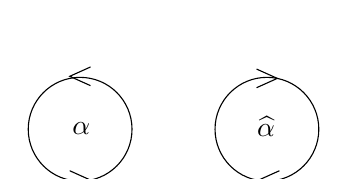
\begin{tikzpicture}[x=0.75pt,y=0.75pt,yscale=-1,xscale=1]
%uncomment if require: \path (0,438); %set diagram left start at 0, and has height of 438

%Shape: Circle [id:dp7806689159040818] 
\draw   (200,155) .. controls (200,141.19) and (211.19,130) .. (225,130) .. controls (238.81,130) and (250,141.19) .. (250,155) .. controls (250,168.81) and (238.81,180) .. (225,180) .. controls (211.19,180) and (200,168.81) .. (200,155) -- cycle ;
%Shape: Circle [id:dp8696260691285458] 
\draw   (110,155) .. controls (110,141.19) and (121.19,130) .. (135,130) .. controls (148.81,130) and (160,141.19) .. (160,155) .. controls (160,168.81) and (148.81,180) .. (135,180) .. controls (121.19,180) and (110,168.81) .. (110,155) -- cycle ;
\draw   (130,175) -- (140,179.5) -- (130,184) ;
\draw   (220,126) -- (230,130.5) -- (220,135) ;
\draw   (140,134) -- (130,129.5) -- (140,125) ;
\draw   (231,184) -- (221,179.5) -- (231,175) ;

% Text Node
\draw (130,150.4) node [anchor=north west][inner sep=0.75pt]    {$\alpha $};
% Text Node
\draw (219,147.4) node [anchor=north west][inner sep=0.75pt]    {$\widehat{\alpha }$};
\end{tikzpicture}
\end{center}

In general, we have the following definition. 

\begin{defn}
Let $\Gamma \subseteq \R^2$ and $[a, b] \subseteq \R$ be a closed interval. A smooth vector-valued 
function 
\[ \alpha : [a, b] \to \Gamma : t \mapsto (\alpha_1(t), \alpha_2(t)) \] 
is called a {\bf smooth parametrization of $\Gamma$} if the following conditions hold:
\begin{enumerate}[(1)]
    \item The image of $\alpha$ is $\Gamma$; that is, $\alpha([a, b]) = \Gamma$.
    \item The {\bf velocity vector} $\alpha'(t) = (\alpha'_1(t), \alpha'_2(t))$ is non-zero 
    for all $t \in [a, b]$.
    \item If $\alpha(a) = \alpha(b)$, then $\alpha'(a) = \alpha'(b)$.
\end{enumerate}
\end{defn}

\begin{center}
\tikzset{every picture/.style={line width=0.75pt}} %set default line width to 0.75pt        

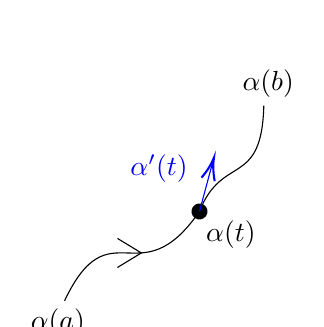
\begin{tikzpicture}[x=0.75pt,y=0.75pt,yscale=-1,xscale=1]
%uncomment if require: \path (0,438); %set diagram left start at 0, and has height of 438

%Curve Lines [id:da435510613996984] 
\draw    (139.5,140) .. controls (161.5,94) and (175.5,139) .. (204.5,97) ;
\draw [shift={(204.5,97)}, rotate = 304.62] [color={rgb, 255:red, 0; green, 0; blue, 0 }  ][fill={rgb, 255:red, 0; green, 0; blue, 0 }  ][line width=0.75]      (0, 0) circle [x radius= 3.35, y radius= 3.35]   ;
\draw   (165,110) -- (176.5,117) -- (165,124) ;
%Curve Lines [id:da9708124340491926] 
\draw    (204.5,97) .. controls (215.5,69) and (234.5,86) .. (235.5,46) ;
%Straight Lines [id:da11945207870584196] 
\draw [color={rgb, 255:red, 0; green, 0; blue, 255 }  ,draw opacity=1 ][fill={rgb, 255:red, 74; green, 144; blue, 226 }  ,fill opacity=1 ]   (204.5,97) -- (210.98,72.93) ;
\draw [shift={(211.5,71)}, rotate = 465.07] [color={rgb, 255:red, 0; green, 0; blue, 255 }  ,draw opacity=1 ][line width=0.75]    (10.93,-3.29) .. controls (6.95,-1.4) and (3.31,-0.3) .. (0,0) .. controls (3.31,0.3) and (6.95,1.4) .. (10.93,3.29)   ;

% Text Node
\draw (122,142.4) node [anchor=north west][inner sep=0.75pt]    {$\alpha ( a)$};
% Text Node
\draw (206.5,100.4) node [anchor=north west][inner sep=0.75pt]    {$\alpha ( t)$};
% Text Node
\draw (224,27.4) node [anchor=north west][inner sep=0.75pt]    {$\alpha ( b)$};
% Text Node
\draw (170,68.4) node [anchor=north west][inner sep=0.75pt]    {\textcolor{blue}{$\alpha '( t)$}};

\end{tikzpicture}
\end{center}

Recall that the velocity vector $\alpha'(t)$ is tangent to $\Gamma$ at the point $\alpha(t)$ 
whenever it is non-zero. Condition (2) therefore ensures that one can specify a tangent direction 
to $\Gamma$ at every point. Moreover, if $\alpha(a) = \alpha(b) = z_0$, then the curve $\Gamma$ 
is {\bf closed} (or a {\bf loop}), and condition (3) ensures that there is a well-defined 
tangent direction to $\Gamma$ at $z_0$.

\begin{defn}
A parametrization $\alpha : [a, b] \to \Gamma \subseteq \R^2$ is said to be {\bf simple} 
if the restrictions of $\alpha$ to the intervals $[a, b)$ and $(a, b]$ are both one-to-one.
\end{defn}

Note that if $\alpha$ is not closed, this is equivalent to $\alpha$ being injective on $[a, b]$. 

If a parametrization $\alpha$ is simple, then the curve $\Gamma$ does not self-intersect. 
This is a very important property of curves that admit simple parametrizations. 
The curve on the left is simple, whereas the curve on the right is not.
\begin{center}
\tikzset{every picture/.style={line width=0.75pt}} %set default line width to 0.75pt        

\begin{tikzpicture}[x=0.75pt,y=0.75pt,yscale=-1,xscale=1]
%uncomment if require: \path (0,142); %set diagram left start at 0, and has height of 142

%Curve Lines [id:da26175572006071035] 
\draw    (111.74,34.09) .. controls (18.5,31) and (15.66,96.97) .. (64.09,77.65) .. controls (112.52,58.33) and (90.65,94.7) .. (113.3,94.7) .. controls (135.96,94.7) and (128.15,75) .. (144.55,81.06) .. controls (160.95,87.12) and (168.5,44) .. (111.74,34.09) -- cycle ;
%Curve Lines [id:da33030303097760094] 
\draw    (224.23,19.69) .. controls (256.5,11) and (254.69,77.27) .. (285.94,54.54) .. controls (317.19,31.81) and (226.57,39.39) .. (228.13,70.45) .. controls (229.7,101.52) and (245.32,102.28) .. (264.85,83.34) ;
\end{tikzpicture}
\end{center}

Note that if the parametrization $\alpha$ is only one-to-one on the open interval 
$(a, b)$, then the curve $\Gamma$ can still self-intersect; it is important that 
it is also one-to-one on $a$ or $b$, as we will see in the following example.

\begin{exmp}
Consider the smooth parametrization of the curve $\alpha$ given by 
\[ \alpha : [0, 4\pi] \to \R : t \mapsto \begin{cases} (\cos t - 1, \sin t), & t \in [0, 2\pi] \\
(1 - \cos t, \sin t), & t \in (2\pi, 4\pi]. \end{cases} \]
It is a smooth parametrization of the figure-eight $\Gamma$, which self-intersects even though 
$\alpha$ is one-to-one on $(0, 4\pi)$ (check this).

\begin{center}
\tikzset{every picture/.style={line width=0.75pt}} %set default line width to 0.75pt        

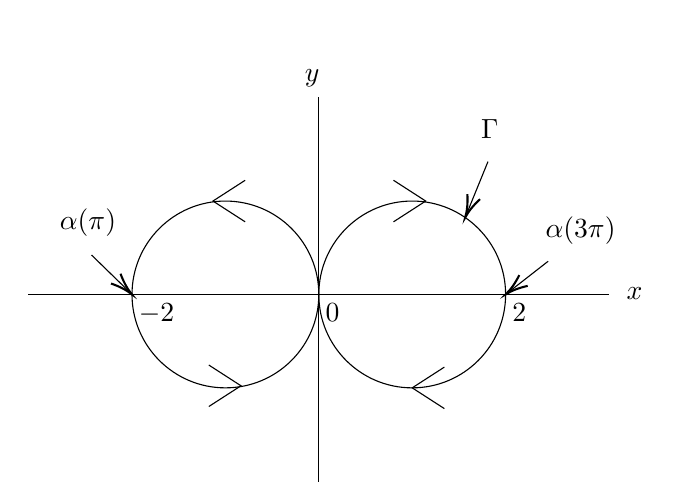
\begin{tikzpicture}[x=0.75pt,y=0.75pt,yscale=-1,xscale=1]
%uncomment if require: \path (0,334); %set diagram left start at 0, and has height of 334

%Straight Lines [id:da8372280773707774] 
\draw    (50,125) -- (330,125) ;
%Straight Lines [id:da7723025368192742] 
\draw    (190,30) -- (190,220) ;
%Shape: Circle [id:dp11216742908684796] 
\draw   (190,125) .. controls (190,100.15) and (210.15,80) .. (235,80) .. controls (259.85,80) and (280,100.15) .. (280,125) .. controls (280,149.85) and (259.85,170) .. (235,170) .. controls (210.15,170) and (190,149.85) .. (190,125) -- cycle ;
%Shape: Circle [id:dp15270954931704273] 
\draw   (100,125) .. controls (100,100.15) and (120.15,80) .. (145,80) .. controls (169.85,80) and (190,100.15) .. (190,125) .. controls (190,149.85) and (169.85,170) .. (145,170) .. controls (120.15,170) and (100,149.85) .. (100,125) -- cycle ;
%Straight Lines [id:da7841082532702541] 
\draw    (80.5,106) -- (98.57,123.6) ;
\draw [shift={(100,125)}, rotate = 224.26] [color={rgb, 255:red, 0; green, 0; blue, 0 }  ][line width=0.75]    (10.93,-3.29) .. controls (6.95,-1.4) and (3.31,-0.3) .. (0,0) .. controls (3.31,0.3) and (6.95,1.4) .. (10.93,3.29)   ;
%Straight Lines [id:da4665750034915719] 
\draw    (300.5,109) -- (281.58,123.77) ;
\draw [shift={(280,125)}, rotate = 322.03] [color={rgb, 255:red, 0; green, 0; blue, 0 }  ][line width=0.75]    (10.93,-3.29) .. controls (6.95,-1.4) and (3.31,-0.3) .. (0,0) .. controls (3.31,0.3) and (6.95,1.4) .. (10.93,3.29)   ;
%Straight Lines [id:da9947698733276449] 
\draw    (271.5,61) -- (261.25,86.15) ;
\draw [shift={(260.5,88)}, rotate = 292.17] [color={rgb, 255:red, 0; green, 0; blue, 0 }  ][line width=0.75]    (10.93,-3.29) .. controls (6.95,-1.4) and (3.31,-0.3) .. (0,0) .. controls (3.31,0.3) and (6.95,1.4) .. (10.93,3.29)   ;
\draw   (226,70) -- (241.5,80) -- (226,90) ;
\draw   (137,159) -- (152.5,169) -- (137,179) ;
\draw   (250.5,180) -- (235,170) -- (250.5,160) ;
\draw   (154.5,90) -- (139,80) -- (154.5,70) ;

% Text Node
\draw (182,15.4) node [anchor=north west][inner sep=0.75pt]    {$y$};
% Text Node
\draw (337,120.4) node [anchor=north west][inner sep=0.75pt]    {$x$};
% Text Node
\draw (192,128.4) node [anchor=north west][inner sep=0.75pt]    {$0$};
% Text Node
\draw (102,128.4) node [anchor=north west][inner sep=0.75pt]    {$-2$};
% Text Node
\draw (282,128.4) node [anchor=north west][inner sep=0.75pt]    {$2$};
% Text Node
\draw (64,82.4) node [anchor=north west][inner sep=0.75pt]    {$\alpha ( \pi )$};
% Text Node
\draw (298,86.4) node [anchor=north west][inner sep=0.75pt]    {$\alpha ( 3\pi )$};
% Text Node
\draw (267,39.4) node [anchor=north west][inner sep=0.75pt]    {$\Gamma $};

\end{tikzpicture}
\end{center}
However, $\alpha$ fails to be one-to-one both on $[0, 4\pi)$ and 
$(0, 4\pi]$ since $\alpha(0) = \alpha(2\pi) = \alpha(4\pi) = (0, 0)$, 
which implies that $\alpha$ is not simple.
\end{exmp}

\begin{defn}
A {\bf piecewise-smooth parametrization} of a subset $\Gamma$ of $\R^2$ is a finite number of subsets 
$\Gamma_0, \dots, \Gamma_{n-1}$ of $\Gamma$ together with smooth parametrizations 
$\alpha_i : [a_i, a_{i+1}] \to \Gamma_i$ for each $0 \leq i \leq n-1$ such that:
\begin{itemize}
    \item $a = a_0 < a_1 < \cdots < a_n = b$, 
    \item $\alpha_i(a_{i+1}) = \alpha_{i+1}(a_{i+1})$ for all $0 \leq i \leq n-1$, and 
    \item $\Gamma = \bigcup_{i=0}^{n-1} \Gamma_i$.
\end{itemize}
\end{defn}

\begin{center}
\tikzset{every picture/.style={line width=0.75pt}} %set default line width to 0.75pt        

\begin{tikzpicture}[x=0.75pt,y=0.75pt,yscale=-1,xscale=1]
%uncomment if require: \path (0,334); %set diagram left start at 0, and has height of 334

%Curve Lines [id:da02074476413630122] 
\draw    (83.5,122) .. controls (123.5,81) and (149.5,90) .. (187.5,115) ;
%Curve Lines [id:da8756718148988389] 
\draw    (187.5,115) .. controls (210.5,175) and (230.5,171) .. (251.5,124) ;
%Curve Lines [id:da2920324572422526] 
\draw    (251.5,124) .. controls (226.5,82) and (331.5,81) .. (328.5,119) ;

% Text Node
\draw (54,122.4) node [anchor=north west][inner sep=0.75pt]    {$\alpha ( a)$};
% Text Node
\draw (181,91.4) node [anchor=north west][inner sep=0.75pt]    {$\alpha ( a_{1})$};
% Text Node
\draw (253.5,127.4) node [anchor=north west][inner sep=0.75pt]    {$\alpha ( a_{2})$};
% Text Node
\draw (330.5,122.4) node [anchor=north west][inner sep=0.75pt]    {$\alpha ( b)$};
% Text Node
\draw (123,73.4) node [anchor=north west][inner sep=0.75pt]    {$\Gamma _{0}$};
% Text Node
\draw (210,164.4) node [anchor=north west][inner sep=0.75pt]    {$\Gamma _{1}$};
% Text Node
\draw (279,70.4) node [anchor=north west][inner sep=0.75pt]    {$\Gamma _{2}$};

\end{tikzpicture}
\end{center}

Finally, a {\bf (piecewise-)smooth parametrized curve} is a pair $(\Gamma, \alpha)$ consisting 
of a subset $\Gamma$ of $\R^2$ together with a (piecewise-)smooth parametrization $\alpha$ of $\Gamma$.

\begin{exmp}
For an example of a piecewise-smooth curve, consider the triangle $\Gamma$ with vertices 
$(0, 0)$, $(1, 0)$ and $(0, 1)$ together with the parametrization 
\[ \alpha : [0, 3] \to \Gamma : t \mapsto \begin{cases} (t, 0), & 0 \leq t \leq 1 \\ 
(2-t, t-1), & 1 \leq t \leq 2 \\ (0, 3-t), & 2 \leq t \leq 3. \end{cases} \]
\end{exmp}

\begin{center}
\tikzset{every picture/.style={line width=0.75pt}} %set default line width to 0.75pt        

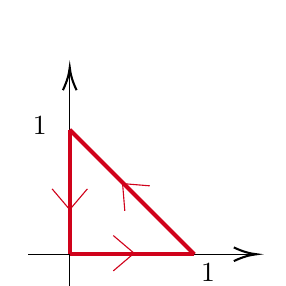
\begin{tikzpicture}[x=0.75pt,y=0.75pt,yscale=-1,xscale=1]
%uncomment if require: \path (0,334); %set diagram left start at 0, and has height of 334

%Straight Lines [id:da04724931373418517] 
\draw    (110,160) -- (110,52) ;
\draw [shift={(110,50)}, rotate = 450] [color={rgb, 255:red, 0; green, 0; blue, 0 }  ][line width=0.75]    (10.93,-3.29) .. controls (6.95,-1.4) and (3.31,-0.3) .. (0,0) .. controls (3.31,0.3) and (6.95,1.4) .. (10.93,3.29)   ;
%Straight Lines [id:da31962906300654126] 
\draw    (90,140) -- (198,140) ;
\draw [shift={(200,140)}, rotate = 180] [color={rgb, 255:red, 0; green, 0; blue, 0 }  ][line width=0.75]    (10.93,-3.29) .. controls (6.95,-1.4) and (3.31,-0.3) .. (0,0) .. controls (3.31,0.3) and (6.95,1.4) .. (10.93,3.29)   ;
%Straight Lines [id:da3660877332667978] 
\draw [color={rgb, 255:red, 208; green, 2; blue, 27 }  ,draw opacity=1 ][fill={rgb, 255:red, 208; green, 2; blue, 27 }  ,fill opacity=1 ][line width=1.5]    (110,80) -- (110,140) ;
%Straight Lines [id:da7478728162413726] 
\draw [color={rgb, 255:red, 208; green, 2; blue, 27 }  ,draw opacity=1 ][fill={rgb, 255:red, 208; green, 2; blue, 27 }  ,fill opacity=1 ][line width=1.5]    (170,140) -- (110,140) ;
%Straight Lines [id:da08595857920203298] 
\draw [color={rgb, 255:red, 208; green, 2; blue, 27 }  ,draw opacity=1 ][fill={rgb, 255:red, 208; green, 2; blue, 27 }  ,fill opacity=1 ][line width=1.5]    (110,80) -- (170,140) ;
\draw  [color={rgb, 255:red, 208; green, 2; blue, 27 }  ,draw opacity=1 ] (131,131) -- (141,139.5) -- (131,148) ;
\draw  [color={rgb, 255:red, 208; green, 2; blue, 27 }  ,draw opacity=1 ] (136.53,119.05) -- (135.46,105.96) -- (148.55,107.03) ;
\draw  [color={rgb, 255:red, 208; green, 2; blue, 27 }  ,draw opacity=1 ] (118.5,108.5) -- (110,118.5) -- (101.5,108.5) ;

% Text Node
\draw (91,72.4) node [anchor=north west][inner sep=0.75pt]    {$1$};
% Text Node
\draw (172,143.4) node [anchor=north west][inner sep=0.75pt]    {$1$};
\end{tikzpicture}
\end{center}

\begin{defn}
A {\bf Jordan curve} is a simple, closed (piecewise-)smooth curve.
\end{defn}

Jordan curves therefore look like loops that do not have self-intersections. 

\begin{exmp}
Circles, triangles, and rectangles are all Jordan curves.
\end{exmp}

\begin{thm}[Jordan Curve Theorem]
If $\Gamma$ is a Jordan curve, its complement $\R^2 \setminus \Gamma$ consists of two disjoint 
domains: one bounded (the "inside"), and one unbounded (the "outside"), each 
domain having the curve $\Gamma$ as its boundary. If a point inside $\Gamma$ is joined 
by a path to a point outside $\Gamma$, then the path must cross $\Gamma$.
\end{thm}
\begin{pf}
Outside the scope of the course.
\end{pf}

\begin{defn}
A {\bf Jordan domain} is a bounded domain $\Gamma \subseteq \R^2$ whose boundary is the union of 
a finite number of {\it positively oriented} Jordan curves, in the sense that when one walks 
along a given curve in the direction specified by its parametrization, then $\Gamma$ always 
lies to the left.
\end{defn}

\begin{center}
\tikzset{every picture/.style={line width=0.75pt}} %set default line width to 0.75pt        

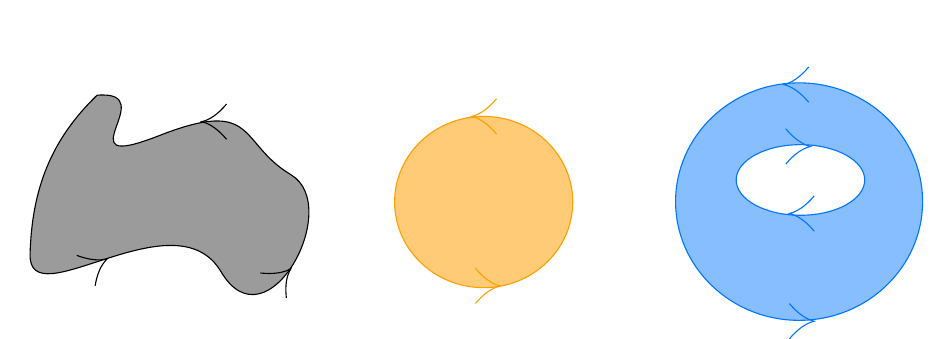
\begin{tikzpicture}[x=0.75pt,y=0.75pt,yscale=-1,xscale=1]
%uncomment if require: \path (0,334); %set diagram left start at 0, and has height of 334

%Curve Lines [id:da4676271183378984] 
\draw [color={rgb, 255:red, 0; green, 0; blue, 0 }  ,draw opacity=1 ][fill={rgb, 255:red, 155; green, 155; blue, 155 }  ,fill opacity=1 ]   (99.79,72.61) .. controls (132.09,70.06) and (81.66,110.89) .. (129.43,92.18) .. controls (177.21,73.46) and (167.48,95.58) .. (193.14,110.89) .. controls (218.8,126.2) and (181.64,195.1) .. (159.52,157.68) .. controls (137.4,120.25) and (66.61,180.64) .. (67.5,149.17) .. controls (68.38,117.69) and (77.67,93.88) .. (99.79,72.61) -- cycle ;
\draw   (162.17,93.88) .. controls (158.19,89.15) and (154.21,86.32) .. (150.23,85.37) .. controls (154.21,84.42) and (158.19,81.59) .. (162.17,76.86) ;
\draw   (178.46,158.27) .. controls (184.74,158.91) and (189.65,158.2) .. (193.16,156.17) .. controls (191.04,159.54) and (190.31,164.25) .. (190.97,170.3) ;
\draw   (89.98,149.78) .. controls (95.88,151.96) and (100.8,152.5) .. (104.74,151.4) .. controls (101.79,154.14) and (99.81,158.5) .. (98.82,164.51) ;
%Shape: Ellipse [id:dp8534618398623988] 
\draw  [color={rgb, 255:red, 255; green, 159; blue, 1 }  ,draw opacity=1 ][fill={rgb, 255:red, 255; green, 192; blue, 89 }  ,fill opacity=0.82 ] (243.13,124.07) .. controls (243.13,101.29) and (262.34,82.82) .. (286.04,82.82) .. controls (309.74,82.82) and (328.95,101.29) .. (328.95,124.07) .. controls (328.95,146.86) and (309.74,165.33) .. (286.04,165.33) .. controls (262.34,165.33) and (243.13,146.86) .. (243.13,124.07) -- cycle ;
\draw  [color={rgb, 255:red, 255; green, 159; blue, 0 }  ,draw opacity=1 ] (292.23,91.32) .. controls (288.25,86.6) and (284.27,83.77) .. (280.29,82.82) .. controls (284.27,81.88) and (288.25,79.04) .. (292.23,74.31) ;
\draw  [color={rgb, 255:red, 255; green, 159; blue, 0 }  ,draw opacity=1 ] (282.06,155.97) .. controls (286.04,160.7) and (290.02,163.54) .. (294,164.48) .. controls (290.02,165.43) and (286.04,168.26) .. (282.06,172.99) ;
%Shape: Ellipse [id:dp9999274371066351] 
\draw  [color={rgb, 255:red, 0; green, 117; blue, 255 }  ,draw opacity=1 ][fill={rgb, 255:red, 134; green, 190; blue, 255 }  ,fill opacity=1 ] (378.5,123.86) .. controls (378.5,92.27) and (405.14,66.66) .. (438,66.66) .. controls (470.86,66.66) and (497.5,92.27) .. (497.5,123.86) .. controls (497.5,155.46) and (470.86,181.07) .. (438,181.07) .. controls (405.14,181.07) and (378.5,155.46) .. (378.5,123.86) -- cycle ;
%Shape: Ellipse [id:dp4431329835013198] 
\draw  [color={rgb, 255:red, 0; green, 117; blue, 255 }  ,draw opacity=1 ][fill={rgb, 255:red, 255; green, 255; blue, 255 }  ,fill opacity=1 ] (407.7,113.44) .. controls (407.7,104.05) and (421.56,96.43) .. (438.66,96.43) .. controls (455.77,96.43) and (469.63,104.05) .. (469.63,113.44) .. controls (469.63,122.84) and (455.77,130.45) .. (438.66,130.45) .. controls (421.56,130.45) and (407.7,122.84) .. (407.7,113.44) -- cycle ;
\draw  [color={rgb, 255:red, 0; green, 117; blue, 255 }  ,draw opacity=1 ] (442.64,76.01) .. controls (438.66,71.28) and (434.68,68.45) .. (430.7,67.51) .. controls (434.68,66.56) and (438.66,63.72) .. (442.64,59) ;
\draw  [color={rgb, 255:red, 0; green, 117; blue, 255 }  ,draw opacity=1 ] (445.3,138.11) .. controls (441.31,133.39) and (437.33,130.55) .. (433.35,129.6) .. controls (437.33,128.66) and (441.31,125.83) .. (445.3,121.1) ;
\draw  [color={rgb, 255:red, 0; green, 117; blue, 255 }  ,draw opacity=1 ] (431.58,88.77) .. controls (435.57,93.5) and (439.55,96.33) .. (443.53,97.28) .. controls (439.55,98.22) and (435.57,101.06) .. (431.58,105.79) ;
\draw  [color={rgb, 255:red, 0; green, 117; blue, 255 }  ,draw opacity=1 ] (433.35,172.99) .. controls (437.34,177.71) and (441.32,180.55) .. (445.3,181.49) .. controls (441.32,182.44) and (437.34,185.27) .. (433.35,190) ;
\end{tikzpicture}
\end{center}

\begin{exmp}~
\begin{enumerate}[(1)]
    \item Open discs with the boundary oriented counter-clockwise are Jordan domains.
    \item The annulus $\Gamma = \{z \in \R^2 : r_1 < |z| < r_2\}$ with the inner circle 
    $|z| = r_1$ oriented clockwise and the outer circle $|z| = r_2$ oriented 
    counter-clockwise is a Jordan domain.
\end{enumerate}
\end{exmp}

\newpage 
\section{Parametrized plane curves and integral calculus in the plane}

\begin{defn}
Let $E : [c, d] \to [a, b]$ be a smooth bijection such that $E'(s) > 0$ for all $s \in [a, b]$. 
We say that $E$ is an {\bf equivalence}.
\end{defn}

Let $E : [c, d] \to [a, b]$ be an equivalence. Note that since $E'(s) > 0$ for all $s \in [c, d]$, it
follows that $E$ is strictly increasing and has a smooth inverse by the Inverse Function Theorem. 

Let $\alpha : [a, b] \to \Gamma \subseteq \R^2$ be a smooth parametrization of a plane curve 
$\Gamma$. Given an equivalence $E : [c, d] \to [a, b]$, we set $\beta = \alpha \circ E$. 
Then $\beta : [c, d] \to \Gamma$ is another smooth parametrization of $\Gamma$ that traverses 
the curve in the same direction as $\alpha$, since $E$ is increasing.

\begin{defn}
We say that two smooth parametrizations $\alpha : [a, b] \to \Gamma$ and $\beta : [a, b] 
\to \Gamma$ of a curve $\Gamma \subseteq \R^2$ are {\bf equivalent} if there exists 
an equivalence $E : [c, d] \to [a, b]$ such that $\beta = \alpha \circ E$.
\end{defn}

\begin{exmp}
Let $\Gamma := \{(x, y) \in \R^2 : y = x^2,\, 1 \leq x \leq 2\}$. 
Then $\alpha : [1, 2] \to \Gamma : t \mapsto (t, t^2)$ and $\beta : [1, 4] \to \Gamma : 
s \mapsto (\sqrt{s}, s)$ are equivalent smooth parametrizations of $\Gamma$ since 
we have $\beta = \alpha \circ E$, where $E : [1, 4] \to [1, 2] : s \mapsto \sqrt{s}$ 
is a smooth bijection with $E'(s) > 0$ for all $s \in [1, 4]$. Note that 
$\alpha'(t) = (1, 2t)$ and 
\[ \beta'(s) = \left( \frac{1}{2\sqrt{s}}, 1 \right) = \frac{1}{2\sqrt{s}} (1, 2\sqrt{s}) 
= E'(s) \alpha'(E(s)) \] 
point in the same direction at every point on $\Gamma$, as $E'(s) > 0$ everywhere.
\end{exmp}

As we see in the above example, the velocity vectors of equivalent parametrizations point in the 
same direction since $E'(s) > 0$ everywhere.

\begin{defn}
Let $\alpha : [a, b] \to \Gamma \subseteq \R^2$ be a smooth parametrized curve and set $\beta : 
[a, b] \to \R^2 : t \mapsto \alpha(a+b-t)$. We then denote by $-\Gamma$ the curve with 
{\bf reverse parametrization} $\beta$.
\end{defn}

Note that $\beta = \alpha \circ F$ where $F : [a, b] \to [a, b] : t \mapsto a+b-t$. 
Although $F$ is a smooth bijection, we have $F'(t) = -1 < 0$ for all 
$t \in [a, b]$, and hence $F$ is {\it not} an equivalence. Nonetheless, $\beta$ is a 
smooth parametrization of $\Gamma$, but 
$\beta'(t) = \alpha'(a+b-t)$ for all $t \in [a, b]$ so that $\beta$ traverses 
$\Gamma$ in the opposite direction of $\alpha$.

\begin{center}
\tikzset{every picture/.style={line width=0.75pt}} %set default line width to 0.75pt        

\begin{tikzpicture}[x=0.75pt,y=0.75pt,yscale=-1,xscale=1]
%uncomment if require: \path (0,334); %set diagram left start at 0, and has height of 334

%Curve Lines [id:da24557942696249335] 
\draw    (136.5,163) .. controls (138.5,115) and (203.5,154) .. (203.5,104) ;
\draw   (160.56,127.93) -- (173.69,133.16) -- (164.93,144.26) ;
%Curve Lines [id:da352613321513636] 
\draw    (294.5,164) .. controls (296.5,116) and (361.5,155) .. (361.5,105) ;
\draw   (333.87,142.33) -- (320.74,137.1) -- (329.5,126) ;

% Text Node
\draw (174,144.4) node [anchor=north west][inner sep=0.75pt]    {$\Gamma $};
% Text Node
\draw (330,146.4) node [anchor=north west][inner sep=0.75pt]    {$-\Gamma $};
% Text Node
\draw (121,164.4) node [anchor=north west][inner sep=0.75pt]    {$\alpha ( a)$};
% Text Node
\draw (191,82.4) node [anchor=north west][inner sep=0.75pt]    {$\alpha ( b)$};
% Text Node
\draw (280,166.4) node [anchor=north west][inner sep=0.75pt]    {$\beta ( b)$};
% Text Node
\draw (347,83.4) node [anchor=north west][inner sep=0.75pt]    {$\beta ( a)$};
\end{tikzpicture}
\end{center}

\begin{exmp}
Consider the unit circle $\Gamma = \{z \in \R^2 : |z| = 1\}$ in $\R^2$ with parametrization 
$\alpha : [0, 2\pi] \to \Gamma : t \mapsto (\cos t, \sin t)$, which traverses $\Gamma$
counter-clockwise. Then $-\Gamma$ is the unit circle parametrized by 
$\beta : [0, 2\pi] \to \Gamma : t \mapsto (\cos(2\pi-t), \sin(2\pi-t)) = (\cos t, -\sin t)$, 
which traverses $\Gamma$ clockwise.
\end{exmp}

\begin{defn}
Let $\alpha : [a, b] \to \Gamma \subseteq \R^2$ be a smooth parametrization of a plane curve. 
For any $s \in [a, b]$, we define the {\bf length of the curve from $\alpha(a)$ to 
$\alpha(s)$} to be 
\[ \int_a^s |\alpha'(t)|\,{\rm d}t. \]
\end{defn}

Note that if $|\alpha'(t)| = 1$ for all $t \in [a, b]$, then the length of the curve from 
$\alpha(a)$ to $\alpha(s)$ is simply 
\[ \int_a^s |\alpha'(t)|\,{\rm d}t = \int_a^s 1\,{\rm d}t = s - a. \]
In other words, $\alpha(s)$ is the point in $\Gamma$ at a distance $s-a$ from the initial point 
$\alpha(a)$. In particular, if $a = 0$, then $\alpha(s)$ is the point on $\Gamma$ 
at distance $s$ from the initial point $\alpha(0)$. As it happens, such a parametrization always 
exists and is called the {\bf arclength parametrization}.

\begin{prop}
Let $\alpha : [a, b] \to \Gamma \subseteq \R^2$ be a smooth parametrization of a plane curve of 
length $L$. Then there exists another parametrization $\sigma : [0, L] \to \Gamma$ that is 
equivalent to $\alpha$ and is such that $|\sigma'(s)| = 1$ for all $s \in [0, L]$.

\begin{center}
\tikzset{every picture/.style={line width=0.75pt}} %set default line width to 0.75pt        
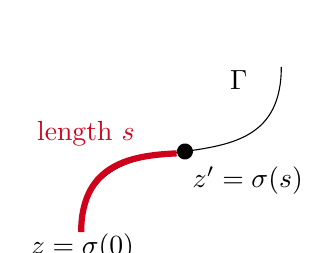
\begin{tikzpicture}[x=0.75pt,y=0.75pt,yscale=-1,xscale=1]
%uncomment if require: \path (0,334); %set diagram left start at 0, and has height of 334

%Curve Lines [id:da24557942696249335] 
\draw    (116.5,185) .. controls (119.38,120.23) and (212.93,172.86) .. (212.93,105.39) ;
\draw [shift={(166.51,146.1)}, rotate = 351.83] [color={rgb, 255:red, 0; green, 0; blue, 0 }  ][fill={rgb, 255:red, 0; green, 0; blue, 0 }  ][line width=0.75]      (0, 0) circle [x radius= 3.35, y radius= 3.35]   ;
%Curve Lines [id:da055728582975171914] 
\draw [color={rgb, 255:red, 208; green, 2; blue, 27 }  ,draw opacity=1 ][line width=2.25]    (116.5,185) .. controls (116.5,151) and (142.5,148) .. (162.5,147) ;

% Text Node
\draw (186.96,105.68) node [anchor=north west][inner sep=0.75pt]    {$\Gamma $};
% Text Node
\draw (91,184.4) node [anchor=north west][inner sep=0.75pt]    {$z=\sigma ( 0)$};
% Text Node
\draw (169,152.4) node [anchor=north west][inner sep=0.75pt]    {$z'=\sigma ( s)$};
% Text Node
\draw (94,130.4) node [anchor=north west][inner sep=0.75pt]    {$\textcolor[rgb]{0.82,0.01,0.11}{\text{length} \ s}$};
\end{tikzpicture}
\end{center}
\end{prop}
\begin{pf}
For all $\tau \in [a, b]$, set 
\[ F(\tau) = \int_a^\tau |\alpha'(t)|\,{\rm d}t. \]
Then $F(a) = 0$ and $F(b) = L$. Moreover, by the Fundamental Theorem of Calculus, we have 
$F'(\tau) = |\alpha'(\tau)|$ for all $\tau \in [a, b]$. In particular, 
this means that $F'(\tau) > 0$ for all $\tau$ since $\alpha'(\tau) \neq 0$ for all $\tau$. 
Hence, by the Inverse Function Theorem, $F$ is invertible with smooth inverse on $[a, b]$. 
Let $E : [0, L] \to [a, b]$ be its inverse, which is also smooth and is such that 
\[ E'(s) = \frac{1}{F'(E(s))} > 0 \]
for all $s \in [0, L]$. That is, $E$ is an equivalence. Now, define 
\[ \sigma(s) := \alpha(E(s)). \]
Then $\sigma'(s) = \alpha'(E(s)) E'(s)$ by the Chain Rule, so that 
\[ |\sigma'(s)| = |\alpha'(E(s))| \cdot |E'(s)| = F'(E(s)) \cdot E'(s) = 1 \]
for all $s \in [0, L]$, proving the result.
\end{pf}

\begin{exmp}
Let $r > 0$ and consider the circle $C = \{z \in \R^2 : |z| = r\}$, parametrized by 
$\alpha : [0, 2\pi] \to C : t \mapsto (r\cos t, r\sin t)$. Its arclength is 
$L = 2\pi r$ and the equivalent arclength parametrization is given by 
\[ \sigma : [0, 2\pi r] \to C : s \mapsto (r\cos(s/r), r\sin(s/r)). \]
Note that $\sigma'(s) = (-\sin(s/r), \cos(s/r))$ so that $|\sigma'(s)| = 1$ 
for all $s \in [0, 2\pi r]$.
\end{exmp}

\begin{defn}
Given an arclength parametrization $\sigma : [0, L] \to \Gamma \subseteq \R^2$ of a plane curve, 
we set 
\[ T(s) := \sigma'(s) = (\sigma'_1(s), \sigma'_2(s)), \]
which is the {\bf unit tangent vector} to $\Gamma$ at the point $\sigma(s)$, and 
\[ N(s) := (\sigma'_2(s), -\sigma'_1(s)) \]
to be the {\bf outward normal vector} to $\Gamma$ at the point $\sigma(s)$.
\end{defn}

\begin{center}
\tikzset{every picture/.style={line width=0.75pt}} %set default line width to 0.75pt        
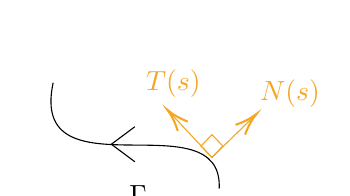
\begin{tikzpicture}[x=0.75pt,y=0.75pt,yscale=-1,xscale=1]
%uncomment if require: \path (0,334); %set diagram left start at 0, and has height of 334

%Curve Lines [id:da352613321513636] 
\draw    (282.5,92) .. controls (270.5,148) and (364.5,99) .. (362.5,143) ;
\draw   (321.88,130.08) -- (310.55,121.63) -- (321.88,113.18) ;
%Straight Lines [id:da4081657722737555] 
\draw [color={rgb, 255:red, 245; green, 166; blue, 35 }  ,draw opacity=1 ]   (359,128) -- (338.87,106.46) ;
\draw [shift={(337.5,105)}, rotate = 406.93] [color={rgb, 255:red, 245; green, 166; blue, 35 }  ,draw opacity=1 ][line width=0.75]    (10.93,-3.29) .. controls (6.95,-1.4) and (3.31,-0.3) .. (0,0) .. controls (3.31,0.3) and (6.95,1.4) .. (10.93,3.29)   ;
%Straight Lines [id:da3096107724840318] 
\draw [color={rgb, 255:red, 245; green, 166; blue, 35 }  ,draw opacity=1 ]   (359,128) -- (379.07,108.4) ;
\draw [shift={(380.5,107)}, rotate = 495.67] [color={rgb, 255:red, 245; green, 166; blue, 35 }  ,draw opacity=1 ][line width=0.75]    (10.93,-3.29) .. controls (6.95,-1.4) and (3.31,-0.3) .. (0,0) .. controls (3.31,0.3) and (6.95,1.4) .. (10.93,3.29)   ;
%Flowchart: Decision [id:dp285667992813607] 
\draw  [color={rgb, 255:red, 245; green, 166; blue, 35 }  ,draw opacity=1 ] (359.01,117) -- (364.25,122.5) -- (359,128) -- (353.75,122.5) -- cycle ;

% Text Node
\draw (318,140.4) node [anchor=north west][inner sep=0.75pt]    {$\Gamma $};
% Text Node
\draw (326,84.4) node [anchor=north west][inner sep=0.75pt]    {$\textcolor[rgb]{0.96,0.65,0.14}{T( s)}$};
% Text Node
\draw (381,89.4) node [anchor=north west][inner sep=0.75pt]    {$\textcolor[rgb]{0.96,0.65,0.14}{N(}\textcolor[rgb]{0.96,0.65,0.14}{s}\textcolor[rgb]{0.96,0.65,0.14}{)}$};
\end{tikzpicture}\end{center}

Note that $N(s)$ and $T(s)$ are orthogonal with respect to the standard inner product $\R^2$, since 
$N(s)$ is obtained by rotating $T(s)$ clockwise by $90^\circ$. Therefore, if $\Gamma$ is 
the boundary of a Jordan domain, then $N(s)$ points outwards of the domain, which is why it is called the
outward normal vector.

\begin{exmp}
Let $r > 0$ and consider the circle $C = \{z \in \R^2 : |z| = r\}$ with arclength parametrization 
given by $\sigma : [0, 2\pi r] \to C : s \mapsto (r \cos(s/r), r\sin(s/r))$. Then 
$T(s) = (-\sin(s/r), \cos(s/r))$ and $N(s) = (\cos(s/r), \sin(s/r))$. 

\begin{center}
\tikzset{every picture/.style={line width=0.75pt}} %set default line width to 0.75pt        

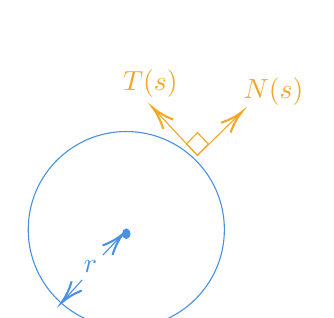
\begin{tikzpicture}[x=0.75pt,y=0.75pt,yscale=-1,xscale=1]
%uncomment if require: \path (0,334); %set diagram left start at 0, and has height of 334

%Straight Lines [id:da4081657722737555] 
\draw [color={rgb, 255:red, 245; green, 166; blue, 35 }  ,draw opacity=1 ]   (374,137) -- (353.87,115.46) ;
\draw [shift={(352.5,114)}, rotate = 406.93] [color={rgb, 255:red, 245; green, 166; blue, 35 }  ,draw opacity=1 ][line width=0.75]    (10.93,-3.29) .. controls (6.95,-1.4) and (3.31,-0.3) .. (0,0) .. controls (3.31,0.3) and (6.95,1.4) .. (10.93,3.29)   ;
%Straight Lines [id:da3096107724840318] 
\draw [color={rgb, 255:red, 245; green, 166; blue, 35 }  ,draw opacity=1 ]   (374,137) -- (394.07,117.4) ;
\draw [shift={(395.5,116)}, rotate = 495.67] [color={rgb, 255:red, 245; green, 166; blue, 35 }  ,draw opacity=1 ][line width=0.75]    (10.93,-3.29) .. controls (6.95,-1.4) and (3.31,-0.3) .. (0,0) .. controls (3.31,0.3) and (6.95,1.4) .. (10.93,3.29)   ;
%Flowchart: Decision [id:dp285667992813607] 
\draw  [color={rgb, 255:red, 245; green, 166; blue, 35 }  ,draw opacity=1 ] (374.01,126) -- (379.25,131.5) -- (374,137) -- (368.75,131.5) -- cycle ;
%Shape: Circle [id:dp7750794190436381] 
\draw  [color={rgb, 255:red, 74; green, 144; blue, 226 }  ,draw opacity=1 ] (292.5,172.75) .. controls (292.5,146.65) and (313.65,125.5) .. (339.75,125.5) .. controls (365.85,125.5) and (387,146.65) .. (387,172.75) .. controls (387,198.85) and (365.85,220) .. (339.75,220) .. controls (313.65,220) and (292.5,198.85) .. (292.5,172.75) -- cycle ;
%Flowchart: Connector [id:dp7090319400029061] 
\draw  [color={rgb, 255:red, 74; green, 144; blue, 226 }  ,draw opacity=1 ][fill={rgb, 255:red, 74; green, 144; blue, 226 }  ,fill opacity=1 ][line width=0.75]  (341.25,174.75) .. controls (341.25,173.65) and (340.58,172.75) .. (339.75,172.75) .. controls (338.92,172.75) and (338.25,173.65) .. (338.25,174.75) .. controls (338.25,175.85) and (338.92,176.75) .. (339.75,176.75) .. controls (340.58,176.75) and (341.25,175.85) .. (341.25,174.75) -- cycle ;
%Straight Lines [id:da16268917924889026] 
\draw [color={rgb, 255:red, 74; green, 144; blue, 226 }  ,draw opacity=1 ]   (328.5,185) -- (336.87,176.2) ;
\draw [shift={(338.25,174.75)}, rotate = 493.57] [color={rgb, 255:red, 74; green, 144; blue, 226 }  ,draw opacity=1 ][line width=0.75]    (10.93,-3.29) .. controls (6.95,-1.4) and (3.31,-0.3) .. (0,0) .. controls (3.31,0.3) and (6.95,1.4) .. (10.93,3.29)   ;
%Straight Lines [id:da5075551743026958] 
\draw [color={rgb, 255:red, 74; green, 144; blue, 226 }  ,draw opacity=1 ]   (318.5,197) -- (309.85,206.52) ;
\draw [shift={(308.5,208)}, rotate = 312.27] [color={rgb, 255:red, 74; green, 144; blue, 226 }  ,draw opacity=1 ][line width=0.75]    (10.93,-3.29) .. controls (6.95,-1.4) and (3.31,-0.3) .. (0,0) .. controls (3.31,0.3) and (6.95,1.4) .. (10.93,3.29)   ;

% Text Node
\draw (337,94.4) node [anchor=north west][inner sep=0.75pt]    {$\textcolor[rgb]{0.96,0.65,0.14}{T( s)}$};
% Text Node
\draw (395,98.4) node [anchor=north west][inner sep=0.75pt]    {$\textcolor[rgb]{0.96,0.65,0.14}{N(}\textcolor[rgb]{0.96,0.65,0.14}{s}\textcolor[rgb]{0.96,0.65,0.14}{)}$};
% Text Node
\draw (318,186.4) node [anchor=north west][inner sep=0.75pt]  [color={rgb, 255:red, 74; green, 144; blue, 226 }  ,opacity=1 ]  {$r$};

\end{tikzpicture}
\end{center}
\end{exmp}

Note that the unit normal vector will come up when we see Green's Theorem.

We now study integral calculus in the plane. Let $[a, b]$ be a closed interval in $\R$ 
and $f : [a, b] \to \R$ be a continuous real-valued function. Recall that 
$f$ is then integral on $[a, b]$ so that 
\[ \int_a^b f(t)\,{\rm d}t \]
exists and is a real number called the {\bf definite integral of $f$ over $[a, b]$}. 
We list some properties of definite integrals. If $f, g \in C^0([a, b])$, then 
\begin{enumerate}[(1)]
    \item $\int_a^b f(t)\,{\rm d}t = \int_a^{t_0} f(t)\,{\rm d}t + \int_{t_0}^b f(t)\,{\rm d}t$ 
    for all $t_0 \in [a, b]$;
    \item $\int_a^b (f+g)(t)\,{\rm d}t = \int_a^b f(t)\,{\rm d}t + \int_a^b g(t)\,{\rm d}t$; 
    \item $\int_a^b Cf(t)\,{\rm d}t = C\int_a^b f(t)\,{\rm d}t$ for all $C \in \R$; and 
    \item $\int_a^b f(t)\,{\rm d}t = -\int_b^a f(t)\,{\rm d}t$.
\end{enumerate}
Properties (2) and (3) tell us that integrals are linear, whereas property (1) tells us that 
the integral over $[a, b]$ is equal to the sum of integrals over the subintervals 
$[a, t_0]$ and $[t_0, b]$.

Suppose now that we want to integrate a continuous vector-valued function $f : \R^2 \to \R^2 : 
(x, y) \mapsto (p(x,y), q(x,y))$ along a curve. How can we set this up?

\begin{defn}
Let $\alpha : [a, b] \to \Gamma \subseteq \R^2$ be a smooth parametrization of a plane curve 
in a domain $\Omega \subseteq \R^2$, and suppose that $p, q : \Omega \to \R$ are 
continuous. We define 
\[ \int_\Gamma p\,{\rm d}x + q\,{\rm d}y := \int_a^b p(\alpha(t)) \alpha'_1(t)\,{\rm d}t 
+ \int_a^b q(\alpha(t)) \alpha'_2(t)\,{\rm d}t. \]
This quantity is called the {\bf line integral of the vector-valued function 
$(p, q) : \Omega \to \R^2 : (x, y) \mapsto (p(x,y), q(x,y))$ along $\Gamma$}.
\end{defn}

Note that these integrals are well-defined since $p(\alpha(t))\alpha'_1(t)$ and $q(\alpha(t))
\alpha'_2(t)$ are both smooth on $[a, b]$. Moreover, since $(p, q) : \Omega \to \R^2$ can be 
interpreted as a vector field in $\R^2$, the line integral $\int_\Gamma p\,{\rm d}x + q\,{\rm d}y$
is also called the {\bf line integral of the vector field $F = (p, q)$ along $\Gamma$}.

\begin{exmp}
Let $(p, q) = (x^2, 1-y)$ and $\Gamma = \{(x, y) \in \R^2 : x^2 + y^2 = 1\}$ be parametrized 
by $\alpha : [0, 2\pi] \to \Gamma : t \mapsto (\cos t, \sin t)$. Then 
$\alpha'(t) = (-\sin t, \cos t)$, and 
\[ \int_\Gamma p\,{\rm d}x + q\,{\rm d}y = \int_0^{2\pi} (\cos t)^2 (-\sin t)\,{\rm d}t 
+ \int_0^{2\pi} (1-\sin t)\cos t\, {\rm d}t = 0. \]
\end{exmp}

Note that one obtains the same value if one uses a parametrization $\beta : [c, d] \to \Gamma$ 
that is equivalent to $\alpha$. Indeed, if $\beta$ is such a parametrization, then 
$\beta = \alpha \circ E$ for some equivalence $E : [c, d] \to [a, b]$. We verify that 
\[ \int_a^b p(\alpha(t)) \alpha'_1(t)\,{\rm d}t = \int_c^d p(\beta(s))\beta'_1(s)\,{\rm d}s. 
\tag{$\star$} \]
If $t = E(s)$, then ${\rm d}t = E'(s)\,{\rm d}s$ and $\beta'(s) = \alpha'(E(s)) E'(s)$ so that
\[ (\beta'_1(s), \beta'_2(s)) = (\alpha'_1(E(s))E'(s), \alpha'_2(E(s))E'(s)), \]
and moreover, 
\[ p(\alpha(t))\alpha'_1(t)\,{\rm d}t = p(\alpha(E(s))) \alpha'_1(E(s)) E'(s)\,{\rm d}s 
= p(\beta(s)) \beta'_1(s)\,{\rm d}s. \]
Since $a = E(c)$ and $b = E(d)$, the above change of variable formula gives $(\star)$. 
A similar computation gives 
\[ \int_a^b q(\alpha(t)) \alpha'_2(t)\,{\rm d}t = \int_c^d q(\beta(s)) \beta'_2(s)\,{\rm d}s. \]
Thus, line integrals are independent of the parametrization up to equivalence.

\begin{exmp}
In Example 3.12, if $\Gamma$ is parametrized instead by the equivalent parametrization 
$\beta : [0, \pi] \to \Gamma : t \mapsto (\cos 2t, \sin 2t)$, then 
$\beta'(t) = (-2\sin 2t, 2\cos 2t)$, so we obtain
\[ \int_\Gamma p\,{\rm d}x + q\,{\rm d}y = \int_0^\pi (\cos 2t)^2 (-2\sin2t)\,{\rm d}t 
+ \int_0^\pi (1-\sin2t)(2\cos2t)\,{\rm d}t = 0. \]
\end{exmp}
Line integrals over piecewise-smooth curves are defined as the sum of the integrals 
over the smooth pieces. More precisely, we have the following definition.

\begin{defn}
Let $(\Gamma, \alpha)$ be a piecewise-smooth parametrized curve in a domain $\Omega \subseteq \R^2$
given by the smooth parametrizations $\alpha_i : [a_i, a_{i+1}] \to \Gamma_i$ for each $0 \leq i \leq 
n-1$. For any two continuous functions $p, q : \Omega \to \R$, the {\bf line integral 
of $(p, q) : \Omega \to \R^2$ along $\Gamma$} is defined as
\[ \int_\Gamma p\,{\rm d}x + q\,{\rm d}y := \int_{\Gamma_0} p\,{\rm d}x + q\,{\rm d}y
+ \int_{\Gamma_1} p\,{\rm d}x + q\,{\rm d}y + \cdots + \int_{\Gamma_{n-1}} p\,{\rm d}x + q\,{\rm d}y. \]
\end{defn}

\begin{exmp}
Consider $(p, q) = (x^2y, x)$, and let $\Gamma$ be the triangle with vertices 
$(0, 0)$, $(1, 0)$, and $(0, 1)$ with piecewise-smooth parametrization 
\[ \alpha : [0, 3] \to \Gamma : t \mapsto \begin{cases} (t, 0), & 0 \leq t \leq 1, \\
(2-t, t-1), & 1\leq t \leq 2, \\ (0, 3-t), & 2 \leq t \leq 3. \end{cases} \]
In this case, $(\Gamma, \alpha)$ is the union of the three line segments 
\begin{align*}
    \alpha_0 : [0, 1] \to \Gamma_0 : t &\mapsto (t, 0), \\
    \alpha_1 : [1, 2] \to \Gamma_1 : t &\mapsto (2-t, t-1), \\
    \alpha_2 : [2, 3] \to \Gamma_2 : t &\mapsto (0, 3-t).
\end{align*}
We then have 
\[ \int_{\Gamma_0} p\,{\rm d}x + q\,{\rm d}y = \int_0^1 p(t, 0) \cdot 1 \, {\rm d}t = 0 \] 
since $\alpha'_0(t) = (1, 0)$ and $p(t, 0) = 0$. Then, since 
$\alpha'_1(t) = (-1, 1)$, we have 
\[ \int_{\Gamma_1} p\,{\rm d}x + q\,{\rm d}y = \int_1^2 p(2-t, t-1) \cdot (-1)\,{\rm d}t 
+ \int_1^2 q(2-t, t-1) \cdot 1 \, {\rm d}t = 5/12. \]
Finally, we see that 
\[ \int_{\Gamma_2} p\,{\rm d}x + q\,{\rm d}y = \int_2^3 q(0, 3-t) \cdot (-1) \,{\rm d}t = 0 \] 
since $\alpha'_2(t) = (0, -1)$ and $q(0, 3-t) = 0$. Putting these together, we obtain 
\[ \int_\Gamma p\,{\rm d}x + q\,{\rm d}y = 0 + 5/12 + 0 = 5/12. \]
\end{exmp}

We list some properties of line integrals. 

\begin{prop}
Let $\alpha : [a, b] \to \Gamma \subseteq \R^2$ be a piecewise-smooth parametrization of a 
plane curve in a domain $\Omega \subseteq \R^2$, and let $p, q, p_1, p_2, q_1, q_2 : 
\Omega \to \R$ be continuous. Moreover, let $C, C' \in \R$. Then
\begin{enumerate}[(1)]
    \item $\int_\Gamma (p_1+p_2)\,{\rm d}x + (q_1+q_2)\,{\rm d}y = 
    \int_\Gamma p_1\,{\rm d}x + q_1\,{\rm d}y + \int_\Gamma p_2\,{\rm d}x + q_2\,{\rm d}y$;
    \item $\int_\Gamma Cp\,{\rm d}x + C'q\,{\rm d}y = C\int_\Gamma p\,{\rm d}x + C'
    \int_\Gamma q\,{\rm d}y$; and 
    \item $\int_{-\Gamma} p\,{\rm d}x + q\,{\rm d}y = -\int_\Gamma p\,{\rm d}x + q\,{\rm d}y$.
\end{enumerate}
\end{prop}
\begin{pf}
This follows straight from the definition and the properties of definite integrals;
we leave the proof as an exercise.
\end{pf}

What happens if $p\,{\rm d}x + q\,{\rm d}y = {\rm d}u$ for some $u \in C^1(\Omega)$, 
in which case it is called {\bf exact}? In other words, 
\[ p\,{\rm d}x + q\,{\rm d}y = u_x\,{\rm d}x = u_y\,{\rm d}y = {\rm d}u \]
so that $p = u_x$ and $q = u_y$. Then by the Chain Rule, we have 
\begin{align*}
    \frac{{\rm d}}{{\rm d}t} (u(\alpha(t))) 
    &= \frac{\rm d}{{\rm d}t} (u(\alpha_1(t), \alpha_2(t))) \\
    &= u_x(\alpha(t)) \alpha'_1(t) + u_y(\alpha(t)) \alpha'_2(t) \\
    &= p(\alpha(t))\alpha'_1(t) + q(\alpha(t)) \alpha'_2(t),
\end{align*}
which implies that 
\[ \int_\Gamma p\,{\rm d}x + q\,{\rm d}y = \int_a^b \frac{\rm d}{{\rm d}t} (u(\alpha(t)))\,{\rm d}t 
= u(\alpha(b)) - u(\alpha(a)) = u(z_2) - u(z_1). \]
Hence, $\int_\Gamma p\,{\rm d}x + q\,{\rm d}y$ depends only on the endpoints of $\Gamma$
when $p\,{\rm d}x + q\,{\rm d}y$ is exact; that is, it is {\bf independent of path}.
We can summarize the above discussion with the following theorem.

\begin{thm}
Let $\Gamma \subseteq \R^2$ be a piecewise-smooth curve from $z_1$ to $z_2$ lying inside a domain 
$\Omega \subseteq \R^2$. Moreover, let $u \in C^1(\Omega)$. Then 
\[ \int_\Gamma {\rm d}u = u(z_2) - u(z_1). \]
In particular, if $\Gamma$ is a loop so that $z_2 = z_1$, then $\int_\Gamma {\rm d}u = 0$.
\end{thm}

\begin{exmp}
Recall Example 3.12 where we had $(p, q) = (x^2, 1-y)$. Observe that $p\,{\rm d}x + q\,{\rm d}y$ is 
exact, since 
\[ p\,{\rm d}x + q\,{\rm d}y = x^2\,{\rm d}x = (1-y)\,{\rm d}y = {\rm d}\left(\frac13x^3 - \frac12(1-y)^2
\right) = {\rm d}u. \]
Thus, it is not surprising that the integral we computed was $0$ as we were integrating 
${\rm d}u$ along a loop; namely, the circle $\Gamma = \{(x, y) \in \R^2 : x^2+y^2=1\}$.
\end{exmp}

As a consequence of Theorem 3.17, we see that if there exists a loop $\Gamma \subseteq \R^2$ 
along which 
\[ \int_\Gamma p\,{\rm d}x + q\,{\rm d}y \neq 0, \]
then $p\,{\rm d}x + q\,{\rm d}y$ cannot be exact. That is, there does not exist 
$u \in C^1(\Omega)$ such that $p\,{\rm d}x + q\,{\rm d}y = {\rm d}u$. For instance, we 
saw in Example 3.15 that with $(p, q) = (x^2 y, x)$ and a loop $\Gamma$, 
we had $\int_\Gamma p\,{\rm d}x + q\,{\rm d}y = 5/12 \neq 0$. Hence, 
$p\,{\rm d}x + q\,{\rm d}y$ is not exact on $\R^2$.

\newpage 
\section{More integral calculus on the plane}

Let $\Omega$ be a bounded subset of $\R^2$ and let $f : \Omega \to \R$ be continuous. 
Then $f$ is integrable on $\Omega$ so that 
\[ \iint_\Omega f(x, y)\,{\rm d}x\,{\rm d}y \]
exists and is a real number called the {\bf double integral of $f$ over $\Omega$}.

We recall some properties of the double integral. Let $f, g \in C^0(\Omega)$ and 
$C \in \R$. 
\begin{itemize}
    \item We have $\iint_\Omega (Cf+g)(x, y)\,{\rm d}x\,{\rm d}y = C \iint_\Omega f(x, y)\,{\rm d}x
    \,{\rm d}y + \iint_\Omega g(x, y)\,{\rm d}x\,{\rm d}y$. 
    \item If $f(z) > 0$ for all $z \in \Omega$, then $\iint_\Omega f(x, y)\,{\rm d}x\,{\rm d}y > 0$. 
    This also holds by replacing $>$ with $\geq$.
\end{itemize}
Another useful property that will come up on more than one occasion when we study harmonic functions 
is the Bump Principle. 

\begin{prop}[Bump Principle]
Let $\Omega$ be a bounded domain in $\R^2$ and $q : \Omega \to \R$ be a continuous function. Moreover, 
assume that $q(z) \geq 0$ for all $z \in \Omega$. Then $q$ is identically zero on $\Omega$ 
if and only if 
\[ \iint_\Omega q(x, y)\,{\rm d}x\,{\rm d}y = 0. \]
\end{prop}
\begin{pf}
If $q$ is identically zero on $\Omega$, then clearly $\iint_\Omega q(x,y)\,{\rm d}x\,{\rm d}y = 0$. 
Conversely, suppose that we have $\iint_\Omega q(x,y)\,{\rm d}x\,{\rm d}y = 0$. Towards a contradiction, 
suppose that there exists $z_0 \in \Omega$ such that $q(z_0) > 0$. By the continuity of $q$, 
there exists an open neighbourhood $W$ of $z_0$ contained in $\Omega$ such that 
$q(w) > 0$ for all $w \in W$. In particular, we have that $\iint_W q(x,y)\,{\rm d}x\,{\rm d}y > 0$.
Moreover, $\iint_{\Omega\setminus W} q(x,y)\,{\rm d}x\,{\rm d}y \geq 0$ since 
$q(z) \geq 0$ for all $z \in \Omega \setminus W$. It follows that 
\[ 0 = \iint_\Omega q(x,y)\,{\rm d}x\,{\rm d}y = \iint_W q(x,y)\,{\rm d}x\,{\rm d}y 
+ \iint_{\Omega\setminus W} q(x,y)\,{\rm d}x\,{\rm d}y > 0, \]
which is a contradiction. Thus, $q$ is identically zero on $\Omega$.
\end{pf}

\begin{defn}
Let $k$ be a positive integer. A Jordan domain $\Omega \subseteq \R^2$ is said to be 
{\bf $k$-connected} if its boundary consists of $k$ distinct Jordan curves. 
Note that this is equivalent to its complement $\R^2 \setminus \Omega$ consisting of $k$ 
disjoint connected components. In particular, if $\Omega$ is $1$-connected (so that 
it has "no holes" inside), then it is called {\bf simply connected}.
\end{defn}

\begin{exmp}~
\begin{enumerate}[(1)]
    \item Discs, triangles, and squares are simply connected.
    \item The annulus $\Omega = \{z \in \R^2 : r_1 < |z| < r_2\}$ is $2$-connected.
    \item The domain $\Omega = D(0; 4) \setminus (\overline{D}(-2; 1) \cup \overline{D}(1; 2))$ 
    is $3$-connected.
\end{enumerate}
\end{exmp}

\begin{thm}[Green's Theorem]
Let $\Omega \subseteq \R^2$ be a $k$-connected Jordan domain and suppose that $p, q \in C^1(\Omega^+)$, 
where $\Omega^+$ is a domain containing $\Omega$ and $\partial \Omega$. Then 
\[ \int_{\partial\Omega} p\,{\rm d}x + q\,{\rm d}y = \iint_\Omega (q_x - p_y)\,{\rm d}x\,{\rm d}y. \]
\end{thm}
\begin{pf}
The proof reduces to proving the two equalities 
\begin{align*}
    \iint_{\partial\Omega} p\,{\rm d}x &= - \iint_\Omega p_y\,{\rm d}x\,{\rm d}y, \tag{1} \\ 
    \iint_{\partial\Omega} q\,{\rm d}y &= \iint_\Omega q_x\,{\rm d}x\,{\rm d}y, \tag{2}
\end{align*}
since these must hold when $q = 0$ and $p = 0$, respectively.

We prove the theorem in the case where $\Omega$ is a rectangle; that is, 
\[ \Omega = \{z \in \R^2 : a < x < b,\, c < x < d\}. \]
The boundary $\partial\Omega$ of $\Omega$ consists of four line segments $\Gamma_1$, 
$\Gamma_2$, $\Gamma_3$, and $\Gamma_4$ oriented as in the following diagram so that 
$\partial\Omega$ is positively oriented.

\begin{center}
\tikzset{every picture/.style={line width=0.75pt}} %set default line width to 0.75pt        

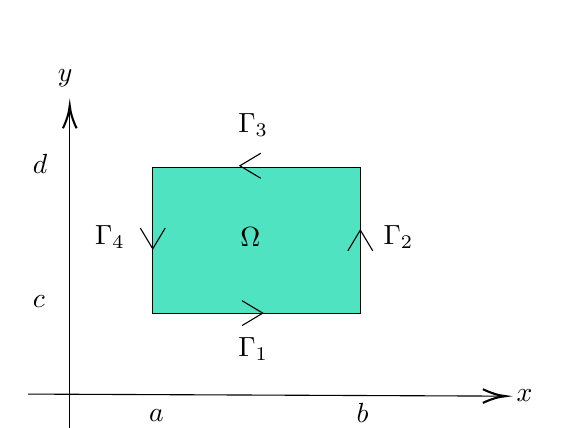
\begin{tikzpicture}[x=0.75pt,y=0.75pt,yscale=-1,xscale=1]
%uncomment if require: \path (0,334); %set diagram left start at 0, and has height of 334

%Straight Lines [id:da6164451716993042] 
\draw    (92,177) -- (320,177.99) ;
\draw [shift={(322,178)}, rotate = 180.25] [color={rgb, 255:red, 0; green, 0; blue, 0 }  ][line width=0.75]    (10.93,-3.29) .. controls (6.95,-1.4) and (3.31,-0.3) .. (0,0) .. controls (3.31,0.3) and (6.95,1.4) .. (10.93,3.29)   ;
%Straight Lines [id:da980709989310449] 
\draw    (112,198) -- (112,40) ;
\draw [shift={(112,38)}, rotate = 450] [color={rgb, 255:red, 0; green, 0; blue, 0 }  ][line width=0.75]    (10.93,-3.29) .. controls (6.95,-1.4) and (3.31,-0.3) .. (0,0) .. controls (3.31,0.3) and (6.95,1.4) .. (10.93,3.29)   ;
%Shape: Rectangle [id:dp8913053407509322] 
\draw  [fill={rgb, 255:red, 80; green, 227; blue, 194 }  ,fill opacity=1 ] (152,68) -- (252,68) -- (252,138) -- (152,138) -- cycle ;
\draw   (195,132) -- (205,138) -- (195,144) ;
\draw   (158,97) -- (152,107) -- (146,97) ;
\draw   (204,73) -- (194,67) -- (204,61) ;
\draw   (246,108) -- (252,98) -- (258,108) ;

% Text Node
\draw (149,183.4) node [anchor=north west][inner sep=0.75pt]    {$a$};
% Text Node
\draw (249,180.4) node [anchor=north west][inner sep=0.75pt]    {$b$};
% Text Node
\draw (93,128.4) node [anchor=north west][inner sep=0.75pt]    {$c$};
% Text Node
\draw (93,60.4) node [anchor=north west][inner sep=0.75pt]    {$d$};
% Text Node
\draw (193,95.4) node [anchor=north west][inner sep=0.75pt]    {$\Omega $};
% Text Node
\draw (192,148.4) node [anchor=north west][inner sep=0.75pt]    {$\Gamma _{1}$};
% Text Node
\draw (262,94.4) node [anchor=north west][inner sep=0.75pt]    {$\Gamma _{2}$};
% Text Node
\draw (192,40.4) node [anchor=north west][inner sep=0.75pt]    {$\Gamma _{3}$};
% Text Node
\draw (123,94.4) node [anchor=north west][inner sep=0.75pt]    {$\Gamma _{4}$};
% Text Node
\draw (326,173.4) node [anchor=north west][inner sep=0.75pt]    {$x$};
% Text Node
\draw (105,19.4) node [anchor=north west][inner sep=0.75pt]    {$y$};
\end{tikzpicture}
\end{center}

Let us prove (1). First, note that 
\[ \iint_\Omega p_y\,{\rm d}x\,{\rm d}y = \int_a^b \left( \int_c^d p_y\,{\rm d}y \right){\rm d}x 
= \int_a^b (p(x, d) - p(x, c))\,{\rm d}x. \]
Moreover, we have 
\[ \int_{\partial\Omega} p\,{\rm d}x = \int_{\Gamma_1} p\,{\rm d}x + \int_{\Gamma_2} p\,{\rm d}x
+ \int_{\Gamma_3} p\,{\rm d}x + \int_{\Gamma_4} p\,{\rm d}x. \]
To compute $\int_{\partial\Omega} p\,{\rm d}x$, we need to parametrize the line segments 
$\Gamma_1$, $\Gamma_2$, $\Gamma_3$, and $\Gamma_4$, and compute the corresponding line integrals. 
Indeed, consider the parametrizations 
\begin{align*}
    \alpha &: [a, b] \to \Gamma_1 : x \mapsto (x, c), \\
    \beta &: [c, d] \to \Gamma_2 : y \mapsto (b, y), \\
    \gamma &: [a, b] \to \Gamma_3 : x \mapsto (a+b-x, d), \\
    \delta &: [c, d] \to \Gamma_4 : y \mapsto (a, c+d-y).
\end{align*}
Then $p(\alpha(x)) \alpha'_1(x)\,{\rm d}x = p(x, c) \cdot 1 \,{\rm d}x$ on $\Gamma_1$ so that 
\[ \int_{\Gamma_1} p\,{\rm d}x = \int_a^b p(x, c)\,{\rm d}x. \] 
On the other hand, we have $p(\gamma(x)) \gamma'_1(x)\,{\rm d}x = p(a+b-x, d) \cdot (-1)\,{\rm d}x$
on $\Gamma_3$, and hence 
\[ \int_{\Gamma_3} p\,{\rm d}x = -\int_a^b p(a+b-x, d)\,{\rm d}x = -\int_a^b p(x, d)\,{\rm d}x, \]
where the second equality follows from the substitution $u = a+b-x$. Finally, 
$\beta_1$ and $\delta_1$ are constant on $\Gamma_2$ and $\Gamma_4$ respectively, so we have 
$\beta'_1 = \delta'_1 = 0$, which implies that $p(\beta(x))\beta'_1(x) = p(\delta(x)) \delta'_1(x) 
= 0$ and $\int_{\Gamma_2} p\,{\rm d}x = \int_{\Gamma_4} p\,{\rm d}x = 0$. Putting it all 
together, we get 
\[ \int_{\partial\Omega} p\,{\rm d}x = \int_a^b p(x, c)\,{\rm d}x + 0 - \int_a^b p(x, d)\,{\rm d}x 
+ 0 = \int_a^b (p(x, c) - p(x, d))\,{\rm d}x, \]
which yields (1). The equality (2) can be proved in a similar fashion, and is left as an exercise.
\end{pf}

\begin{exmp}
Let us verify Green's Theorem with an example. Let 
\[ \Omega = \{z \in \R^2 : x^2 \leq y \leq 1\}. \]
In particular, $\Omega$ is the domain bounded by $\Gamma_1 = \{z \in \R^2 : y = x^2,\, -1 \leq 
x \leq 1\}$ and $\Gamma_2 = \{z \in \R^2 : y = 1,\, -1 \leq x \leq 1\}$. Let us orient the boundary 
of $\Omega$ positively by parametrizing $\Gamma_1$ and $\Gamma_2$ with 
\begin{align*}
    \alpha &: [-1, 1] \to \Gamma_1 : t \mapsto (t, t^2), \\ 
    \beta &: \;\;\, [1, 3] \to \Gamma_2 : t \mapsto (2-t, 1).
\end{align*}
Consider the differential $p\,{\rm d}x + q\,{\rm d}y = x^2y\,{\rm d}x - x\,{\rm d}y$, which satisfies 
the hypotheses of Green's Theorem since $p = x^2y$ and $q=-x$ are both smooth in $\R^2$. 
We wish to verify that 
\[ \int_{\partial\Omega} p\,{\rm d}x + q\,{\rm d}y = \iint_\Omega (q_x - p_y)\,{\rm d}x\,{\rm d}y. 
\tag{$\star$} \]
First, we compute the right-hand side of $(\star)$. Note that $q_x - p_y = -(1+x^2)$. It then 
follows that 
\begin{align*}
    \iint_\Omega (q_x - p_y)\,{\rm d}x\,{\rm d}y 
    &= \int_{-1}^1 \int_{x^2}^1 -(1+x^2)\,{\rm d}y\,{\rm d}x \\
    &= \int_{-1}^1 -(1+x^2)y \, \Big|_{y=x^2}^1\,{\rm d}x \\
    &= \int_{-1}^1 x^4 - 1 \,{\rm d}x \\
    &= \frac{x^5}5 - x\, \Big|_{x=-1}^1 = -\frac85.
\end{align*}
For the left-hand side of $(\star)$, we have 
\[ \int_{\partial\Omega} p\,{\rm d}x + q\,{\rm d}y 
= \int_{\Gamma_1} p\,{\rm d}x + q\,{\rm d}y + \int_{\Gamma_2} p\,{\rm d}x + q\,{\rm d}y. \]
On $\Gamma_1$, we see that $x=t$ and $y=t^2$ so that ${\rm d}x = {\rm d}t$ and 
${\rm d}y = 2t\,{\rm d}t$. Hence, we get 
\begin{align*}
    \int_{\Gamma_1} p\,{\rm d}x + q\,{\rm d}y 
    &= \int_{-1}^1 (t)^2(t^2)\,{\rm d}t + \int_{-1}^1 (-t) \cdot 2t\,{\rm d}t \\
    &= \int_{-1}^1 t^4 - 2t^2\,{\rm d}t = -\frac{14}{15}.
\end{align*}
On the other hand, on $\Gamma_2$, we have $x = 2-t$ and $y = 1$ so that ${\rm d}x = 
(-1)\,{\rm d}t$ and ${\rm d}y = 0$. Thus, we obtain 
\begin{align*}
    \int_{\Gamma_2} p\,{\rm d}x + q\,{\rm d}y 
    &= \int_1^3 (2-t)(1)\cdot (-1)\,{\rm d}t + \int_1^3 (t-2) \cdot 0\,{\rm d}t \\
    &= -\int_1^3 (2-t)^2\,{\rm d}t = -\frac23.
\end{align*}
Combining these results, we therefore have 
\[ \int_{\partial\Omega} p\,{\rm d}x + q\,{\rm d}y = -\frac{14}{15} - \frac23 = -\frac85 
= \iint_\Omega (q_x - p_y)\,{\rm d}x\,{\rm d}y, \]
which verifies Green's Theorem in this case.
\end{exmp}

We will see many consequences of Green's Theorem when we study harmonic functions. Nonetheless, 
we can already state two important consequences.
\begin{itemize}
    \item {\bf Path independence.} One can use Green's Theorem to obtain a shorter proof of the 
    fact that the line integral of an exact form ${\rm d}u$ on a loop is always zero 
    (as in Lecture 3), in the case where $u$ is of class $C^2$.
    \item {\bf Poincar\'e Lemma.} Another consequence is known as the Poincar\'e Lemma, 
    which states that if $p, q \in C^1(\Omega)$ for a {\it simply connected} domain 
    $\Omega$, then $p\,{\rm d}x + q\,{\rm d}y$ is exact if and only if $p_y = q_x$.
\end{itemize}
We leave the proofs of both of these results to Assignment 2, but we note that the forward 
direction of the Poincar\'e Lemma was proved on Assignment 1.

\newpage
\section{Outward normal vector, harmonic functions in the plane}

Given an arclength parametrization $\sigma : [0, L] \to \Gamma \subseteq \R^2$ of a plane 
curve, recall that the unit tangent and outward normal vectors to $\Gamma$ at the point 
$\sigma(s)$ are defined, respectively, as 
$T(s) := \sigma'(s) = (\sigma'_1(s), \sigma'_2(s))$ and $N(s) := (\sigma'_2(s), -\sigma'_1(s))$. 

If $z_0 = \sigma(s_0)$ for some $s_0 \in [0, L]$, we set $N(z_0) := N(s_0)$. 
Consider a function $u : \Omega \to \R$ on a domain $\Omega \subseteq \R^2$, 
and assume that its gradient 
\[ \nabla u = (u_x, u_y) \]
is defined on $\Omega$. We set 
\[ \frac{\partial u}{\partial n}(z_0) := \nabla u(z_0) \cdot N(z_0). \]

\begin{remark}
If $u$ is differentiable at $z_0$, then $\frac{\partial u}{\partial n}(z_0)$ is the 
directional derivative of $u$ in the direction $N(z_0)$ and is equal to the rate of 
change of $u$ as one moves away from $z_0$ in the direction $N(z_0)$.
\end{remark}

\begin{exmp}
Consider the circle $C = \{z \in \R^2 : |z| = r\}$ of radius $r > 0$, with 
arclength parametrization $\sigma : [0, 2\pi r] \to C : s \mapsto (r\cos(s/r), r\sin(s/r))$. 
We saw in Example 3.10 that $N(s) = (\cos(s/r), \sin(s/r))$. 
Now, let $u \in C^1(\R^2)$. Then 
\[ \frac{\partial u}{\partial n} = u_x \cos(s/r) + u_y \sin(s/r). \]
In fact, we have $\frac{\partial u}{\partial n} = \frac{\partial u}{\partial r}$. Indeed, 
in terms of polar coordinates $z = (r\cos t, r\sin t)$, observe that 
\[ \frac{\partial u(r, t)}{\partial r} = \frac{\partial}{\partial r} (u(r\cos t, r\sin t)) 
= u_x \cos t + u_y \sin t. \] 
It then follows that $\frac{\partial u}{\partial n} = u_x \cos(s/r) + u_y \sin(s/r) 
= \frac{\partial u}{\partial r}$ on $C$.
\end{exmp}

\begin{remark}
In general, we have 
\[ \frac{\partial u}{\partial n} \dd s = -u_y \dd x + u_x \dd y. \]
To see this, first note that
\begin{align*}
    \frac{\partial u}{\partial n}(\sigma(s)) &= \nabla u(\sigma(s)) \cdot N(\sigma(s)) \\
    &= (u_x(\sigma(s)), u_y(\sigma(s))) \cdot (\sigma'_2(s), -\sigma'_1(s)) \\
    &= -u_y (\sigma(s)) \sigma'_1(s) + u_x(\sigma(s)) \sigma'_2(s).
\end{align*}
Therefore, we see that 
\[ \frac{\partial u}{\partial n}(\sigma(s))\dd s = -u_y(\sigma(s)) \sigma'_1(s)\dd s 
+ u_x(\sigma(s)) \sigma'_2(s)\dd s. \]
Now, notice that on $\Gamma$, we have $z = (\sigma_1(s), \sigma_2(s))$ so that 
${\rm d}x = \sigma'_1(s)\dd s$ and ${\rm d}y = \sigma'_2(s) \dd s$. Thus, 
we obtain the desired formula 
\[ \frac{\partial u}{\partial n} \dd s = -u_y \dd x + u_x \dd y. \]
\end{remark}

As a direct corollary of Green's Theorem, we have the following result. 

\begin{thm}[Inside-Outside Theorem]
Let $\Omega \subseteq \R^2$ be a $k$-connected Jordan domain, and let 
$u \in C^2(\Omega^+)$ for some domain $\Omega^+$ containing $\Omega$ and $\partial\Omega$. Then 
\[ \int_{\partial\Omega} \frac{\partial u}{\partial n}\dd s = \iint_\Omega \Delta u \dd x \dd y, \]
where $\Delta u = u_{xx} + u_{yy}$ is the Laplacian of $u$.
\end{thm}
\begin{pf}
First, note that since $u \in C^2(\Omega^+)$, the partials $u_x$ and $u_y$ of $u$ exist 
and are of class $C^1$ on $\Omega^+$. Recall from Remark 5.3 that 
\[ \frac{\partial u}{\partial n} \dd s = -u_y \dd x + u_x \dd y \]
on $\partial\Omega$. Moreover, by Green's Theorem with $p = -u_y$ and $q = u_x$, we obtain 
\[ \int_{\partial\Omega} -u_y \dd x + u_x \dd y = \iint_\Omega ((u_x)_x - (-u_y)_y)\dd x \dd y 
= \iint_\Omega \Delta x \dd x \dd y. \qedhere \]
\end{pf}

We will now focus on harmonic functions as we noted in Lecture 1. The Inside-Outside Theorem 
will be quite important in this regard. 

\begin{defn}
Let $u \in C^2(\Omega)$ for some domain $\Omega \subseteq \R^2$. We say that $u$ is 
{\bf harmonic} if $\Delta u = 0$, where $\Delta u := u_{xx} + u_{yy}$ is the {\bf Laplacian} of $u$.
\end{defn}

In other words, harmonic functions are solutions to the {\bf Laplace equation} $u_{xx} + u_{yy} = 0$.

\begin{exmp}~
\begin{enumerate}[(1)]
    \item Constant functions are harmonic on $\R^2$.
    \item Linear polynomials are harmonic on $\R^2$. Indeed, suppose $u(x, y) = ax+by+c$ for some 
    $a, b, c \in \R$. Then $u_{xx} = u_{yy} = 0$ so that $\Delta u = 0$. 
    \item The function $u(x, y) = Ae^x \cos y + Be^x \sin y$ is harmonic on $\R^2$ for all 
    $A, B \in \R$. 
    \item Linear combinations of harmonic functions are harmonic. That is, 
    if $u$ and $v$ are harmonic on a domain $\Omega \subseteq \R^2$, then so is 
    $Au+v$ for all $A \in \R$. 
    \item Products of harmonic functions might not be harmonic. For instance, 
    it follows from (2) that $u(x, y) = x$ is harmonic, but 
    $v(x, y) = (u(x, y))^2 = x^2$ is not.
\end{enumerate}
We leave it as an exercise to check that (3), (4), and (5) hold. 
\end{exmp}

The Laplace equation is a very important equation that has many applications in mathematics and 
physics. We will see later that the real and complex parts of differentiable complex functions 
are harmonic. 

We now give a very useful characterization of harmonic functions in terms of line integrals.

\begin{thm}
Let $\Omega \subseteq \R^2$ be a domain and let $u \in C^2(\Omega)$. Then 
$u$ is harmonic in $\Omega$ if and only if for every Jordan curve $\Gamma \subseteq \R^2$ 
inside $\Omega$ whose interior lies in $\Omega$, we have 
\[ \int_\Gamma \frac{\partial u}{\partial n}\dd s = 0. \]
\end{thm}
\begin{pf}
Suppose that $u$ is harmonic. Then $\Delta u = 0$, and by the Inside-Outside Theorem, 
if $\Gamma$ is any Jordan curve inside $\Omega$ with interior lying in $\Omega$, then 
\[ \int_\Gamma \frac{\partial u}{\partial n}\dd s = 0. \]
Conversely, suppose that $\int_\Gamma \frac{\partial u}{\partial n}\dd s = 0$ 
for every Jordan curve inside $\Omega$ whose interior lies in $\Omega$. 
Suppose to the contrary that there exists $z_0 \in \Omega$ such that 
$\Delta u(z_0) \neq 0$. Assume without loss of generality that $\Delta u(z_0) > 0$. 
Since $u \in C^2(\Omega)$, we see that $\Delta u$ is continuous on $\Omega$. 
By the continuity of $\Delta u$, there exists an open neighbourhood $W$ of $z_0$ 
contained in $\Omega$ such that $\Delta u(w) > 0$ for all $w \in W$. 
In particular, since $W$ is open, there exists $r > 0$ with $D(z_0; r) \subseteq W \subseteq \Omega$. 
Hence, $\Delta u(z) > 0$ for all $z \in D(z_0; r)$ so that 
\[ \iint_{D(z_0; r)} \Delta u \dd x \dd y > 0. \]
However, the boundary of $D(z_0; r)$ is the circle $C = \{z \in \R^2 : |z - z_0| = r\}$, 
which is a Jordan curve inside $\Omega$ whose interior $D(z_0; r)$ lies inside $\Omega$. 
Moreover, orienting $C$ counter-clockwise making $D(z_0; r)$ into a Jordan domain, 
it follows from the Inside-Outside Theorem that 
\[ \int_C \frac{\partial u}{\partial n}\dd s = \iint_{D(z_0;r)} \Delta u \dd x \dd y > 0, \]
contradicting our hypothesis. Thus, $\Delta u = 0$ everywhere on $\Omega$, and so $u$ is harmonic.
\end{pf}

\newpage 
\section{Mean Value Theorem}

Recall that for a continuous real-valued function of one variable $f : [a, b] \to \R$, the 
Mean Value Theorem (MVT) states that if $f$ is differentiable on $(a, b)$, then there exists 
$c \in (a, b)$ such that 
\[ f'(c) = \frac{f(b) - f(a)}{b-a}, \]
and this value is called the {\bf mean value of $f$ on $[a, b]$}.

There is also an integral version of the MVT which states that if $f$ is continuous on 
$[a, b]$, then there exists $c \in (a, b)$ such that 
\[ f(c) = \frac{1}{b-a} \int_a^b f(t)\dd t. \]
We can see that this is a direct consequence of the MVT. Indeed, for $x \in [a, b]$, let 
\[ F(x) := \int_a^x f(t)\dd t. \]
By the Fundamental Theorem of Calculus, we know that $F$ is continuous on $[a, b]$ and 
differentiable on $(a, b)$, with $F'(x) = f(x)$ for all $x \in (a, b)$. 
Thus, by the MVT, there exists $c \in (a, b)$ such that 
\[ F'(c) = \frac{F(b) - F(a)}{b-a}. \]
Since $F(a) = 0$, $F(b) = \int_a^b f(t) \dd t$, and $F'(c) = f(c)$, this gives 
\[ f(c) = \frac{1}{b-a} \int_a^b f(t)\dd t. \]
Note that $f(c)$ is again interpreted as the average or mean value of $f$ on $[a, b]$. 
We will see that this theorem generalizes to harmonic functions as the 
Circumferential Mean Value Theorem.

The MVT and integral MVT can also be extended for real functions of two variables (and 
more generally, $n$ variables). We only state the integral version of the MVT 
in two variables here. Let $A$ be a connected, compact subset of $\R^2$, 
and let $f$ be a continuous real-valued function on $A$. Then, there exists 
$z_0 \in A$ such that 
\[ f(z_0) = \frac{1}{\area(A)} \iint_A f(x, y)\dd x \dd y, \]
where $\area(A)$ is the area of $A$.

\begin{exmp}
If $A = \overline{D}(z_0; R)$, then $\area(A) = \pi R^2$. Therefore, for any continuous 
real-valued function $u$ on $\overline{D}(z_0; R)$, there exists $\zeta \in \overline{D}(z_0; R)$ 
such that 
\[ u(\zeta) = \frac{1}{\pi R^2} \iint_{D(z_0; r)} u\dd x \dd y. \tag{$1$} \]
We will see that for harmonic functions $u$, equation $(1)$ holds with $\zeta = z_0$ 
for any $z_0$ in the domain $\Omega$ of $u$ and any disc centered at $z_0$ whose domain is in 
$\Omega$. This is known as the Solid Mean Value Theorem, which we will prove at the 
end of this lecture. 
\end{exmp}

Before discussing the Circumferential Mean Value Theorem, we first need to define line integrals 
of continuous scalar functions. 

\begin{defn}
Let $\alpha : [a, b] \to \Gamma$ be a smooth parametrization of a plane curve in a domain 
$\Omega$, and let $f : \Omega \to \R$ be continuous. We define 
\[ \int_\Gamma f(x, y) \dd s := \int_a^b f(\alpha(t)) |\alpha'(t)| \dd t. \]
This quantity is called the {\bf line integral of the scalar function 
$f : \Omega \to \R : (x, y) \mapsto f(x, y)$ along $\Gamma$}.
\end{defn}

Note that these line integrals are well-defined since $f(\alpha(t)) |\alpha'(t)|$ is continuous 
on $[a, b]$. Moreover, if $f$ is the constant function $1$, then 
$\int_\Gamma {\rm d}s = \int_a^b |\alpha'(t)| \dd t$ is the arclength of $\Gamma$.

\begin{exmp}
Consider the circle $C = \{(x, y) \in \R^2 : x^2+y^2 = R^2\}$ parametrized by 
$\alpha : [0, 2\pi] \to C : \theta \mapsto (R\cos\theta, R\sin\theta)$. Then 
$\alpha'(\theta) = (-R\sin\theta, R\cos\theta)$ and $|\alpha'(\theta)| = R$. 
Therefore, for any continuous function $f : \R^2 \to \R$, we have 
$f(\alpha(\theta)) = f(R, \theta)$, and 
\[ \int_C f(x, y)\dd s = \int_0^{2\pi} f(R, \theta) R \dd \theta = 0. \]
\end{exmp}

Note that unlike line integrals of vector-valued functions, one obtains the same value 
for $\int_\Gamma f(x, y) \dd s $ for any parametrization $\alpha : [a, b] \to \Gamma$ 
of the plane curve (not even the orientation matters). 

\begin{prop}
A line integral of a scalar function
along a smooth curve is independent of the parametrization.
\end{prop}
\begin{pf}
Let $\alpha : [a, b] \to \Gamma$ be a smooth parametrization of the curve 
$\Gamma$ inside the domain $\Omega$, and let $f : \Omega \to \R$ be a continuous 
scalar function on $\Omega$. We saw in Lecture 3 that $\alpha$ is equivalent to the 
arclength parametrization $\sigma : [0, L] \to \Gamma$, where $L$ is the length 
of $\Gamma$ and $\sigma$ is such that $|\sigma'(s)| = 1$. 
Therefore, $\alpha = \sigma \circ E$ for some equivalence $E : [a, b] \to [0, L]$. 
Let us verify that
\[ \int_a^b f(\alpha(t))|\alpha'(t)|\dd t = \int_0^L f(\sigma(s)) \dd s. \tag{$2$} \]
Consider the change of variable $s = E(t)$. Then ${\rm d}s = E'(t) \dd t$ and 
$\alpha'(t) = \sigma'(E(t)) E'(t)$ so that 
\[ |\alpha'(t)| = |\sigma'(E(t)) E'(t)| = |\sigma'(E(t))| |E'(t)| = E'(t) \]
as $|\sigma'(E(t))| = 1$ and $E'(t) > 0$ on $[0, L]$. Therefore, we have 
\[ f(\alpha(t)) |\alpha'(t)| \dd t = f(\sigma(E(t))) E'(t) \dd t = 
f(\sigma(s)) \dd s. \]
Since $0 = E(a)$ and $L = E(b)$, we obtain equation $(2)$. Thus, every parametrization 
of $\Gamma$ yields a line integral that is equal to $\int_0^L f(\sigma(s)) \dd s$. 
By construction, the arclength parametrization of $\alpha$ depends only on the 
orientation of $\alpha$, since $\sigma(s)$ is the point on $\Gamma$ at a distance $s$ 
from $\sigma(0) = \alpha(a)$. Therefore, it only remains to check that if we change the 
orientation of $\sigma$, we still obtain the same value for the line integral. 

Consider the curve $-\Gamma$ parametrized by $\tau(r) = \sigma(L-r)$, where $r \in [0, L]$.
Then $\tau'(r) = -\sigma'(L-r)$ so that $|\tau'(r)| = |{-\sigma'(L-r)}|$ and 
\[ \int_{-\Gamma} f(x, y)\dd s = \int_0^L f(\tau(r))|\tau'(r)|\dd r = \int_0^L f(\sigma(L-r))\dd r. \]
Performing the substitution $s = L-r$, we obtain 
\[ \int_{-\Gamma} f(x, y) \dd s = \int_L^0 f(\sigma(s)) (-1)\dd s = \int_0^L f(\sigma(s)) \dd s. \]
Thus, the line integral of the scalar function $f(x, y)$ is independent of the parametrization $\alpha$. 
\end{pf}

We define line integrals of 
scalar functions over piecewise-smooth curves as the sum of the integrals over the 
smooth pieces. More precisely, if $(\Gamma, \alpha)$ is a piecewise-smooth parametrized curve 
over a domain $\Gamma$ given by the smooth parametrizations 
$\alpha_i : [\alpha_i, \alpha_{i+1}] \to \Gamma_i$ for all $0 \leq i \leq n-1$, then for 
any continuous scalar function $f : \Omega \to \R$, the line integral of $f$ 
along $\Gamma$ is defined as 
\[ \int_\Gamma f(x, y)\dd s := \int_{\Gamma_0} f(x, y)\dd s + \int_{\Gamma_1} f(x, y)\dd s 
+ \cdots + \int_{\Gamma_{n-1}} f(x, y)\dd s. \]

\begin{thm}[Circumferential Mean Value Theorem]
Let $u$ be a harmonic function on a domain $\Omega \subseteq \R^2$, let $z_0$ be a point 
in $\Omega$, and suppose that the closed disc $\overline{D} = \overline{D}(z_0; R)$ is contained 
in $\Omega$. Set $C = \partial D = \{z \in \R^2 : |z - z_0| = R\}$. Then 
\[ u(z_0) = \frac{1}{2\pi R} \int_C u(z)\dd s = \frac{1}{2\pi} \int_0^{2\pi} u(R, \theta) \dd \theta, \]
where $C$ is oriented counter-clockwise and $(r, \theta)$ denote polar coordinates 
centered at the point $z_0$. In other words, $u(z_0)$ is the mean value of $u$ 
along the circle $C$.
\end{thm}
\begin{pf}
Before we proceed with the proof, we note that if $z_0 = (x_0, y_0)$, then the polar coordinates 
centered at $z_0$ are given by $x = x_0 + r\cos\theta$ and $y = y_0 + r\sin\theta$ with 
$r > 0$ and $0 \leq \theta \leq 2\pi$. Moreover, $2\pi R$ is the arclength of the circle $C$ 
and plays the role of the length $b-a$ of $[a, b]$ in the integral MVT for real 
one variable functions.

First, observe that since $u$ is harmonic on $\Omega$, we have $\Delta u = 0$ on $\Omega$. 
Let $0 < r \leq R$ and $C_r = \{z \in \R^2 : |z - z_0| = r\}$ be the circle centered at 
$z_0$ of radius $r$. Then $C_r$ and its interior $D(z_0; r)$ are contained in $\Omega$, 
so by the Inside-Outside Theorem, we have 
\[ \int_{C_r} \frac{\partial u}{\partial n} \dd s = \iint_{D(z_0; r)} \Delta u \dd x \dd y = 0. \]
Note that the arclength parametrization of $C_r$ is oriented counter-clockwise; 
that is, we have 
\[ \sigma : [0, 2\pi r] \to C_r : s \mapsto (x_0 + r\cos(s/r), y_0 + r\sin(s/r)), \]
where $z_0 = (x_0, y_0)$. If we use polar coordinates centered at $z_0$ so that 
$x = x_0 + r\cos\theta$ and $y = y_0 + r\sin\theta$, then 
\[ \frac{\partial u}{\partial n} = \frac{\partial u}{\partial r}(r, \theta) \]
on $C_r$ (as we saw in Example 5.2). Moreover, since $\theta = s/r$ on $C_r$, we have that 
$0 \leq \theta \leq 2\pi$ and ${\rm d}s = r\dd\theta$ on $C_r$. Therefore, we see that 
\[ 0 = \int_{C_r} \frac{\partial u}{\partial n}\dd s = \int_0^{2\pi} \frac{\partial u}{\partial r}
(r, \theta)r\dd \theta = r \frac{\rm d}{{\rm d}r} \int_0^{2\pi} u(r, \theta)\dd\theta, \]
or equivalently
\[ \frac{\rm d}{{\rm d}r} \int_0^{2\pi} u(r, \theta)\dd\theta = 0, \] 
which implies that $\int_0^{2\pi} u(r, \theta)\dd\theta$ does not depend on $r$. In particular, 
this means that 
\[ \int_0^{2\pi} u(r, \theta)\dd\theta = \int_0^{2\pi} u(R, \theta)\dd\theta \]
since $0 < r \leq R$, and 
\[ \lim_{r\to0} \int_0^{2\pi} u(r, \theta)\dd\theta = \int_0^{2\pi} u(r, \theta)\dd\theta. \]
On the other hand, by the integral version of the MVT, there exists $\theta_r \in [0, 2\pi]$ 
such that 
\[ u(r, \theta_r) = \frac{1}{2\pi} \int_0^{2\pi} u(r, \theta)\dd\theta. \]
Taking the limit $r \to 0$ on both sides, we obtain $u(z_0)$ on the left, while the 
right side is unchanged. Putting it all together, we have 
\[ u(z_0) = \frac{1}{2\pi} \int_0^{2\pi} u(R, \theta)\dd\theta. \qedhere \]
\end{pf}
We list some applications of the Circumferential Mean Value Theorem.
\begin{itemize}
    \item We can compute line integrals of harmonic functions on circles. For example, 
    suppose we want to evaluate $\int_C \log(x^2+y^2)\dd s$ where $C$ is the circle centered 
    at $z_0 = (1, 5)$ with radius $R = 3$, oriented counter-clockwise. Since $u(x, y) = 
    \log(x^2 + y^2)$ is harmonic on the domain $\R^2 \setminus \{0\}$ (check this) 
    and $\overline{D}((1, 5); 3) \subseteq \R^2 \setminus \{0\}$, the Circumferential MVT 
    tells us that 
    \[ \int_C \log(x^2 + y^2)\dd s = 2\pi(3) u(1, 5) = 6\pi \log(26). \]
    \item We can use the Circumferential MVT to give a new characterization of harmonic functions 
    in terms of line integrals over circles, and to prove the Solid MVT.
\end{itemize}

\begin{defn}
Let $\Omega \subseteq \R^2$ be a domain and let $u \in C^2(\Omega)$. Then $u$ is said to have the 
{\bf circumferential mean value property} in $\Omega$ if for every $z_0 \in \Omega$ and 
every disc $D = D(z_0; R)$ such that $\overline{D} \subseteq \Omega$, we have 
\[ u(z_0) = \frac{1}{2\pi R} \int_{\partial D} u(z)\dd s. \]
\end{defn}

By the Circumferential MVT, harmonic functions have the circumferential mean value property. 
In fact, this property is a sufficient condition for harmonicity.

\begin{thm}
Let $\Omega \subseteq \R^2$ be a domain and let $u \in C^2(\Omega)$. Then $u$ is harmonic 
if and only if it has the circumferential mean value property.
\end{thm}
\begin{pf}
It suffices to prove the backward direction. Suppose that for every $z_0 \in \Omega$ 
and every disc $D = D(z_0; R)$ such that $\overline{D} \subseteq \Omega$, we have 
\[ u(z_0) = \frac{1}{2\pi R} \int_{\partial D} u(z)\dd s. \]
Let $z_0 \in \Omega$ and suppose that $\Delta u(z_0) \neq 0$. Without loss of generality, 
we may assume that $\Delta u(z_0) > 0$ (for otherwise we can work with $-\Delta u(z_0)$). 
By the continuity of $u$, there exists $r' > 0$ such that $\Delta u > 0$ on 
$D(z_0; r')$. In particular, since $\Omega$ is open, we can choose such an $r'$ such that 
$D(z_0; r') \subseteq \Omega$. Choose $r < r'$ and set $D_r = D(z_0; r)$. Then 
$\overline{D}_r \subseteq \Omega$ and by assumption, 
\[ u(z_0) = \frac{1}{2\pi r} \int_{\partial D_r} u(z)\dd s = \frac{1}{2\pi} \int_0^{2\pi} 
u(r, \theta)\dd \theta, \]
where $(r, \theta)$ denote polar coordinates centered at the point $z_0$. Differentiating 
both sides with respect to $r$ and multiplying by $r$, we obtain 
\[ 0 = r \frac{\rm d}{{\rm d}r} \int_0^{2\pi} u(r, \theta)\dd \theta = 
\int_0^{2\pi} \frac{\partial u}{\partial r} (r, \theta)\dd\theta 
= \int_{C_r} \frac{\partial u}{\partial n}\dd s 
= \iint_{D_r} \Delta x \dd x \dd y, \]
where $C_r$ is the circle of radius $r$ and the last equality follows from the Inside-Outside Theorem.
By the Bump Principle, we then have $\Delta u = 0$ on $D_r = D(z_0; r)$, 
contradicting our assumption that $\Delta u(z_0) \neq 0$. Hence, $u$ is harmonic on $\Omega$.
\end{pf}

\begin{remark}
One can actually prove the stronger statement that if $u$ satisfies the circumferential mean 
value property, then $u$ is not only harmonic, but also smooth. Thus, all harmonic functions 
are smooth. 

The proof requires some notions that we do not need in this course, so we will omit it. 
However, we will see a different proof of this fact when studying complex analytic functions.
\end{remark}

\begin{thm}[Solid Mean Value Theorem]
Let $u$ be a harmonic function on a domain $\Omega \subseteq \R^2$, let $z_0$ be a point 
in $\Omega$, and suppose the closed disc $\overline{D} = \overline{D}(z_0; R)$ is contained in 
$\Omega$. Then 
\[ u(z_0) = \frac{1}{\pi R^2} \iint_D u\dd x \dd y. \]
In particular, $u(z_0)$ is the mean value of $u$ over the disc $D$.
\end{thm}
\begin{pf}
By the Circumferential MVT, we know that 
\[ u(z_0) = \frac{1}{2\pi} \int_0^{2\pi} u(r,\theta)\dd\theta \]
for all $0 < r \leq R$. Multiplying both sides by $r\dd r$ and integrating from $r = 0$ 
to $r = R$, we get 
\[ \int_0^R u(z_0)r \dd r = \frac{1}{2\pi} \int_0^R \int_0^{2\pi} u(r, \theta)r\dd \theta \dd r. \]
The left side of the equation gives 
\[ \int_0^R u(z_0)r \dd r = u(z_0) \int_0^R r\dd r = u(z_0) \frac{R^2}2. \]
On the other hand, the right side of the equation is equal to 
\[ \frac{1}{2\pi} \int_0^R \int_0^{2\pi} u(r, \theta)r \dd \theta \dd r = \frac{1}{2\pi} 
\int_0^{2\pi} \int_0^R u(r, \theta)r \dd r \dd\theta \]
by Fubini's Theorem. Therefore, we get 
\[ u(z_0) = \frac{1}{\pi R^2} \int_0^{2\pi} \int_0^R u(r, \theta)r \dd r \dd\theta. \]
However, we have 
\[ \int_0^{2\pi} \int_0^R u(r, \theta)r \dd r \dd\theta = \iint_D u \dd x \dd y. \]
To see this, let us use a polar change of coordinates to express 
$\iint_D u\dd x \dd y$ as an integral in terms of $r$ and $\theta$. Suppose that 
$z_0 = (x_0, y_0)$. Then $D = D(z_0; R) = \{z \in \R^2 : |z - (x_0, y_0)| < R\}$, which 
can be described in polar coordinates by setting $x = x_0 + r\cos\theta$ and 
$y = y_0 + r\sin\theta$. Then $0 \leq \theta \leq 2\pi$, $0 \leq r \leq R$, and 
${\rm d}x \dd y = r\dd r \dd\theta$ by the change of variable formula. Hence, we obtain 
\[ u(z_0) = \frac{1}{\pi R^2} \iint_D u\dd x \dd y. \qedhere \]
\end{pf}

To finish this lecture, we give some applications of the Solid Mean Value Theorem.
\begin{itemize}
    \item We can compute double integrals of harmonic functions over discs. 
    For example, suppose we want to evaluate $\iint_D e^x\cos y \dd x \dd y$ where 
    $D = D((-1, 3); 1/4)$. Since $u(x, y) = e^x \cos y$ is harmonic on $\R^2$ 
    (as noted in Example 5.6), the Solid MVT implies that 
    \[ \iint_D e^x \cos y \dd x \dd y = \pi(1/4)^2 u(-1, 3) = \frac{\pi \cos(3)}{16e}. \]
    \item The Solid MVT can be used to prove Harnack's Inequality, which is a key 
    ingredient in the proof of Liouville's Theorem.
\end{itemize}

\newpage 
\section{Maximum Principle}

Let $f$ be a continuous real-valued function on a compact subset $E$ of $\R^2$. 
Recall that the Extreme Value Theorem states that $f$ attains both its maximum and 
minimum values on $E$, and that they occur either on $\partial E$ or at a critical 
point of $f$ in $E^\circ$. 

For harmonic functions, which are always continuous, we can say much more. This is a result 
of the Strong Maximum Principle and its corollaries. To be precise, we will see the following results:
\begin{itemize}
    \item If $u$ is a non-constant harmonic function on a domain $\Omega \subseteq \R^2$, then 
$u$ reaches its maximum and minimum on $\partial\Omega$ only.
    \item Let $\Omega \subseteq \R^2$ be a bounded domain. 
    If $u$ is continuous on $\overline\Omega$, harmonic on $\Omega$,
    and vanishes on $\partial\Omega$, then $u$ is identically zero on $\Omega$. 
\end{itemize} 
The second point tells us that harmonic functions on bounded domains are completely determined by their
behaviour on the boundary.

\begin{thm}[Strong Maximum Principle]
Let $u$ be a harmonic function on a domain $\Omega \subseteq \R^2$, and suppose that it has a 
maximum or minimum in $\Omega$. Then $u$ is constant.
\end{thm}
\begin{pf}
Without loss of generality, suppose that $u$ has a maximum at $z_0 \in \Omega$ with 
$u(z_0) = c$. Then $u(z) \leq c$ for all $z \in \Omega$. Note that by the continuity of $u$, 
the set $A := u^{-1}(c)$ of points in $\Omega$ where $u$ is equal to $c$ is closed. 
Moreover, we have $A \neq \varnothing$ since $z_0 \in A$. By connectedness of $\Omega$, 
it suffices to show that $A$ is also open, as the only non-empty subset 
of $\Omega$ which is both open and closed is $\Omega$ itself. Since the choice of the point 
$z_0 \in A$ was arbitrary, it is enough to show that there exists $r > 0$ such that 
$D(z_0; r) \subseteq A$. 

Choose $r > 0$ such that $\overline{D}(z_0; r) \subseteq \Omega$ (which is always possible 
since $\Omega$ is open so that $D(z_0; r') \subseteq \Omega$ for some $r' > 0$, 
and we can take $r = r'/2$). Let us verify that $D(z_0; r) \subseteq A$. Suppose that there 
exists $z_1 \in D(z_0; r)$ such that $z_1 \notin A$. In particular, we have 
$u(z_1) < c$. By the continuity of $u$, we see that $u$ is less than $c$ in an 
open disc $D'$ centered at $z_1$ and contained in $D(z_0; r)$. Therefore, $u(z) < c$ for all $z \in D'$, 
which implies that 
\[ \iint_{D'} u\dd x \dd y < \iint_{D'} c \dd x \dd y. \]
Moreover, since $u(z) \leq c$ for all $z \in D(z_0; r) \setminus D'$, we have 
\[ \iint_{D(z_0; r) \setminus D'} u\dd x \dd y \leq \iint_{D(z_0; r) \setminus D'} c\dd x \dd y. \]
Hence, we see that 
\begin{align*}
    \frac{1}{\pi r^2} \iint_{D(z_0; r)} u \dd x \dd y &= 
    \frac{1}{\pi r^2} \left( \iint_{D'} u\dd x \dd y + \iint_{D(z_0; r) \setminus D'} u \dd x \dd y \right) \\
    &< \frac{1}{\pi r^2} \iint_{D(z_0; r)} c\dd x \dd y = c = u(z_0), 
\end{align*}
where the equality follows from the fact that 
\[ \iint_{D(z_0; r)} c \dd x \dd y = c \iint_{D(z_0; r)} 1 \dd x \dd y = c \dot \area(D(z_0; r)) 
= c\pi r^2. \]
But by the Solid MVT, we get 
\[ u(z_0) = \frac{1}{\pi r^2} \iint_{D(z_0; r)} u \dd x \dd y \]
since $u$ is harmonic on $\Omega$, leading to a contradiction. Hence, $u$ is constantly 
equal to $c$ on $D(z_0; r)$, which implies that $D(z_0; r) \subseteq A$. 
\end{pf}

\begin{remark}
Equivalently, the Strong Maximum Principle states that a non-constant function in a domain 
$\Omega \subseteq \R^2$ does not assume its maximum or minimum values on $\Omega$. 
\end{remark}

\begin{remark}
The fact that $\Omega \subseteq \R^2$ is connected (since it is a domain) is essential for the 
result to hold. Indeed, suppose that $\Omega$ is disconnected; that is, 
there exist disjoint open sets $\Omega_1, \Omega_2 \subseteq \R^2$ such that $\Omega = 
\Omega_1 \cup \Omega_2$. Consider the function 
\[ u : \Omega \to \R : z \mapsto \begin{cases} 0 & \text{if } z \in \Omega_1, \\ 
1 & \text{if } z \in \Omega_2. \end{cases} \]
Then $u$ is non-constant and satisfies the Laplace equation at every point in $\Omega$. 
Moreover, $u$ attains its maximum of $1$ on $\Omega_2$ and its minimum of $0$ on 
$\Omega_1$. In particular, $u$ assumes both its maximum and minimum on $\Omega$. 
Nonetheless, this does not contradict the Strong Maximum Principle as $\Omega$ is not connected.
\end{remark}

\begin{thm}[Weak Maximum Principle]
Let $\Omega \subseteq \R^2$ be a bounded domain. Let $u$ be continuous on $\overline\Omega$
and harmonic on $\Omega$. Then either $u$ is constant, or $u$ attains its maximum and 
minimum value over $\overline\Omega$ on $\partial\Omega$ only. 
\end{thm}
\begin{pf}
Note that since $\Omega$ is bounded, so is $\overline\Omega$, which implies that 
$\overline\Omega$ is compact. Since $u$ is continuous on $\overline\Omega$, 
we know by the Extreme Value Theorem that $u$ has a maximum and minimum on $\overline\Omega$, 
which occur either on $\partial\Omega$ or at a critical point of $u$ in $\Omega$. 
If $u$ is non-constant, the Strong Maximum Principle implies that both the maximum and 
minimum must occur on $\partial\Omega$. 
\end{pf}

\begin{exmp}
Consider $u(x, y) = xy$, which is harmonic on $\R^2$. Then $u$ has a maximum of $1$ and 
a minimum of $0$ on the square $\Omega = \{z \in \R^2 : 0 < x, y < 1\}$, which both occur 
on the boundary; in particular, $u(1, 1) = 1$ and $u$ is zero along the $x$-axis and $y$-axis.
\end{exmp}

\begin{remark}~
\begin{enumerate}[(1)]
    \item The Weak Maximum Principle tells us that any non-constant harmonic function on 
    the bounded domain $\Omega \subseteq \R^2$ that is continuous on $\overline\Omega$ 
    does not have critical points in $\Omega$.
    \item Equivalently, the Weak Maximum Principle states that if $\Omega$ is a bounded 
    domain and $u$ is a non-constant function which is continuous on $\overline\Omega$ and 
    harmonic in $\Omega$, then for every point $z_0 \in \Omega$, we have 
    \[ \min_{z \in \partial\Omega} u(z) < u(z_0) < \max_{z \in \partial\Omega} u(z). \]
    \item The boundedness is crucial. For instance, suppose that $u(x, y) = 2x-y$, which is 
    continuous and harmonic on $\R^2$. The maximum and minimum of $u$ are not attained 
    on the upper-half plane $H = \{z \in \R^2 : y > 0\}$, which is unbounded. 
\end{enumerate}
\end{remark}

\begin{thm}
Let $\Omega \subseteq \R^2$ be a bounded domain. Let $u$ and $v$ be functions which are 
continuous on $\overline\Omega$, harmonic on $\Omega$, and equal on $\partial\Omega$ 
(that is, $u(z) = v(z)$ for all $z \in \partial\Omega)$. Then $u = v$ on $\Omega$. In particular, 
harmonic functions on a bounded domain are completely and uniquely determined by their 
behaviour on the boundary.
\end{thm}
\begin{pf}
Since $u$ and $v$ are both continuous on $\overline\Omega$ and harmonic on $\Omega$, 
so is $u-v$. Moreover, $u-v$ vanishes on $\partial\Omega$ since $u$ and $v$ are equal there. 
Suppose that $u - v$ does not vanish identically on $\Omega$; that is, there exists 
$z_0 \in \Omega$ such that $(u - v)(z_0) \neq 0$. Without loss of generality, 
suppose that $(u - v)(z_0) > 0$. This implies that $u-v$ is not constant on 
$\overline\Omega$, so by the Weak Maximum Principle, $u - v$ attains its maximum and 
minimum values on $\partial\Omega$. However, $(u-v)(z) = 0$ for all $z \in \partial\Omega$ 
and $(u - v)(z_0) > 0$, so we see that the maximum value of $u - v$ must lie in 
$\Omega$, a contradiction.
\end{pf}

\begin{remark}~
\begin{enumerate}[(1)]
    \item Setting $v(x, y) = 0$, Theorem 7.7 implies that if $u$ is harmonic on $\Omega$, 
    continuous on $\overline\Omega$, and zero on $\partial\Omega$, then $u$ is identically 
    zero on $\Omega$. 
    \item As with the Weak Maximum Principle, the boundedness of the domain is crucial. 
    For example, take $u(x, y) = 0$ and $v(x, y) = x$ on the domain $\Omega = \{z \in \R^2 : x < 0\}$. 
    Then $u$ and $v$ are both continuous on $\overline\Omega$, harmonic on $\Omega$, 
    and zero on $\partial\Omega$ (which is the $y$-axis). However, $u$ and $v$ are not 
    equal on $\Omega$.
    \item Theorem 7.7 is specific to harmonic functions (although we will see that complex 
    analytic functions have similar properties). Indeed, continuous or smooth 
    functions can agree on the boundary, but not be equal on the domain. 
    For example, $u(x, y) = 1/(2-x^2-y^2)$ and $v(x, y) = x^2 + y^2$ are both 
    smooth on the closed unit disc $\overline{D} = \overline{D}(0; 1)$, 
    and agree on the boundary, which is the unit circle $|z| = 1$. 
    However, they are not equal on the open disc $D = D(0; 1)$ since 
    $u(0, 0) = 1/2$ but $v(0, 0) = 0$.
\end{enumerate}
\end{remark}

\newpage 
\section{Liouville's Theorem}

We consider one last property of harmonic functions before moving on to complex functions. 
This property deals with {\bf entire} functions, which are functions that are 
harmonic on all of $\R^2$. Liouville's Theorem states that bounded entire functions 
are constant. In order to prove this result, we first require Harnack's Inequality.

\begin{thm}[Harnack's Inequality]
Let $D = D(z_0; R)$ be an open disc and let $u$ be a harmonic function on $D$ such that 
$u(z) \geq 0$ for all $z \in D$. Then for all $z \in D$, we have 
\[ 0 \leq u(z) \leq \left( \frac{R}{R-|z-z_0|} \right)^2 u(z_0). \]
\end{thm}
\begin{pf}
Let $z \in D$ and set $D' = D(z; R - |z-z_0|)$. For all $z' \in D'$, we have 
$|z' - z| < R - |z-z_0|$ so that 
\begin{align*}
    |z' - z_0| &\leq |z' - z| + |z - z_0| < (R - |z-z_0|) + |z-z_0| = R. 
\end{align*}
Hence, $D' \subseteq D$. Applying the Solid MVT to the disc $D'$, we obtain 
\[ 0 \leq u(z) = \frac{1}{\pi (R - |z-z_0|)^2} \iint_{D'} u\dd x \dd y. \]
Moreover, since $u \geq 0$ on $D$ and $D' \subseteq D$, we see that 
\[ \iint_{D'} u\dd x \dd y \leq \iint_D u \dd x \dd y = \pi R^2 u(z_0), \]
where the last equality follows from the Solid MVT. Combining these 
inequalities gives the desired result.
\end{pf}

\begin{thm}[Liouville's Theorem]
An entire function that is bounded above or below is constant.
\end{thm}
\begin{pf}
Suppose that $u$ is an entire function. Suppose that 
$u$ is bounded below, so there exists $M \in \R$ such that $u(z) \geq M$ for all $z \in \R^2$. 
Set $v = u - M$ so that $v \geq 0$ on $\R^2$. Moreover, $v$ is harmonic on $\R^2$
and $v$ is constant if and only if $u$ is constant. Therefore, it suffices to 
prove that $v$ is constant. 

Indeed, since $v(z) \geq 0$ for all $z \in \R^2$, we can apply Harnack's Inequality. 
Fix $z_0, z_1 \in \R^2$. For any radius $R > |z_1 - z_0|$, we have that 
\[ 0 \leq v(z_1) \leq \left( \frac{R}{R - |z_1 - z_0|} \right)^2 v(z_0). \]
Since $v$ is harmonic on $\R^2$, Harnack's Inequality holds for any $R > 0$ as large 
as we want as long as $R > |z_1 - z_0|$. In particular, note that 
\[ \lim_{R\to\infty} \left( \frac{R}{R-|z_1 - z_0|} \right)^2 = 1. \]
Since $v(z_0)$ and $v(z_1)$ are fixed constants, we obtain
$v(z_1) \leq v(z_0)$.
Reversing the roles of $z_0$ and $z_1$, we also find that $v(z_0) \leq v(z_1)$,
and hence $v(z_0) = v(z_1)$. Since $z_0$ and $z_1$ were arbitrary, it follows that 
$v$ is constant, and hence so is $u$.

Finally, suppose $u$ is bounded above. Then $-u$ is entire and bounded below.
Hence, $-u$ is constant by what we just showed, which implies that $u$ is also constant.
\end{pf}

Liouville's Theorem is useful as it can help us determine whether or not a given 
non-constant function is harmonic without having to check if it satisfies the Laplace equation. 
In particular, if the non-constant function is defined on all of $\R^2$ and is bounded 
above or below, then it cannot be harmonic. 

\begin{exmp}
Consider $f(x, y) = 1/(1+x^2+y^2)$, which is defined for all $\R^2$, bounded below by $0$, 
and bounded above by $1$. By Liouville's Theorem, $f$ is not harmonic. We can check this explicitly; 
we have 
\[ f_{xx} + f_{yy} = \frac{6x^2 - 2(1+y^2)}{(1+x^2+y^2)^3} + \frac{6y^2 - 2(1+x^2)}{(1+x^2+y^2)^3} 
= \frac{4(x^2+y^2) - 4}{(1+x^2+y^2)^3} \neq 0. \]
\end{exmp}

\newpage
\section{Complex numbers}

Why do we need complex numbers? One reason is to find solutions to certain polynomial equations, 
such as $x^2 + 1 = 0$. We can construct the  complex numbers as a natural extension of the 
real numbers. Recall that $\R$ equipped with the usual operations of addition and 
multiplication is a field. In particular, for all $a, b, c \in \R$, we have 
\begin{enumerate}[(1)]
    \item $a+b=b+a$;
    \item $a+(b+c)=(a+b)+c$;
    \item $ab=ba$;
    \item $a(bc) = (ab)c$;
    \item $(a+b)c = ac +bc$.
\end{enumerate}
Moreover, we know that the additive and multiplicative identities of $\R$ are $0$ and $1$ respectively.

As mentioned above, the polynomial $x^2 + 1 = 0$ has no real solution. Therefore, we need to 
extend our number system to allow such equations to have solutions. 
Indeed, let $i := \sqrt{-1}$ denote a solution to the equation $x^2 + 1 = 0$, and 
note that both $i$ and $-i$ are solutions. Then, this gives rise to the definition of complex numbers. 

\begin{defn}
A {\bf complex number} is an expression of the form $z = a+bi$ where $a,b \in \R$. 
We say that $a$ is the {\bf real part} of $z$, written $a = \Re(z)$, and $b$ 
is the {\bf imaginary part} of $z$, written $b = \Im(z)$. The set of all complex numbers 
is denoted by $\C$. 
\end{defn}

\begin{remark}
Let $z = a+bi \in \C$.
\begin{enumerate}[(1)]
    \item If $b = 0$, then $z = a$ is a real number. In particular, we see that 
    $\R \subseteq \C$, since $a = a+0i \in \C$ for all $a \in \R$. This 
    is a strict subset as $i \notin \R$. 
    \item If $a = 0$, then $z = bi$ is said to be {\bf purely imaginary}. 
\end{enumerate}
\end{remark}

We say that two complex numbers $z = a + bi$ and $w = c+di$ are equal if and only if 
their real and imaginary parts are equal; that is, $a = c$ and $b = d$. 

\begin{remark}
The real numbers are ordered with respect to $>$ (and $\geq$), which gives us the notion of 
a real number being larger than another real number. 
On the other hand, there is no natural ordering on $\C$. Thus, if we write $a > b$, 
this will always imply that $a, b \in \R$.
\end{remark}

Given $z = a+bi,\, w = c+di \in \C$, we define the following operations: 
\begin{align*}
    \text{\bf Addition: } & z+w = (a+bi)+(c+di) := (a+c) + (b+d)i; \\
    \text{\bf Subtraction: } & z-w = (a+bi)-(c+di) := (a-c) + (b-d)i; \\
    \text{\bf Multiplication: } & z\cdot w = (a+bi)(c+di) := (ac-bd) + (ad+bc)i; \\ 
    \text{\bf Division: } & \frac{z}w = \frac{a+bi}{c+di} := \frac{ac+bd}{c^2+d^2} 
    + \frac{bc-ad}{c^2+d^2}i, \text{ where $w \neq 0$.}
\end{align*}
As expected, we have $i^2 = (0+i)(0+i) = -1$. Moreover, we have $(a+bi)(a-bi) = 
a^2 + b^2 = |a+bi|^2 \in \R$. 

\begin{remark}~
\begin{enumerate}[(1)]
    \item The complex numbers $\C$ are closed under the above operations. 
    \item The additive and multiplicative identities of $\C$ are $0$ and $1$ respectively. 
    \item Addition and multiplication of complex numbers is commutative, associative, 
    and distributive. 
\end{enumerate}
\end{remark}

Recall that the Fundamental Theorem of Algebra states that every polynomial with complex 
coefficients has at least one complex root. For example, the second order polynomial 
$az^2 + bz + c$ has real roots 
\[ z = \frac{-b \pm \sqrt{b^2-4ac}}{2a} \in \R \]
if $b^2 - 4ac \geq 0$, and complex roots 
\[ z = \frac{-b \pm i\sqrt{4ac-b^2}}{2a} \in \C \]
if $b^2 - 4ac < 0$. 

Note that every complex number $z = a+bi$ is uniquely determined by its real part $a$ and 
imaginary part $b$, and hence can be uniquely identified with the ordered pair of real 
numbers $(a, b)$. Thus, there is a one-to-one correspondence between complex numbers and points in the 
$xy$-plane. In this context, the $xy$-plane is called the {\bf complex plane} or 
the {\bf $z$-plane}. 

Since real numbers $z = a \in \R$ correspond to points $(a, 0)$ on the $x$-axis, 
the $x$-axis is called the {\bf real axis}. Similarly, the purely imaginary numbers 
$z = bi$ for $b \in \R$ correspond to points $(0, b)$ on the $y$-axis, so the 
$y$-axis is called the {\bf imaginary axis}. From now on, we will refer to the 
point $(a, b)$ representing the complex number $z = a+bi$ as simply the point $z$. 

\begin{defn}
The {\bf modulus} of a complex number $z = a+bi$ is denoted by $|z|$ and is given by 
\[ |z| := \sqrt{a^2 + b^2}. \]
Note that for all $z \in \C$, we have $|z| \geq 0$, and $|z| = 0$ if and only if $z = 0$. 
\end{defn}

Identifying $z = a+bi$ with the point $(a, b)$ on the $xy$-plane, we see that 
\[ |z| = \dist(0, (a, b)) = \dist(0, z). \]
Moreover, if $z_1 = a_1+b_1i$ and $z_2 = a_2+b_2i$, then 
\begin{align*}
    |z_1-z_2| &= |(a_1-a_2)+(b_1-b_2)i| \\
    &= \sqrt{(a_1-a_2)^2 + (b_1-b_2)^2} \\
    &= \dist((a_1, b_1), (a_2, b_2)) \\
    &= \dist(z_1, z_2). 
\end{align*}
In particular, if $z_0 \in \C$ and $R$ is a positive real number, then the set 
$\{z \in \C : |z-z_0| = R\}$ corresponds to the points in the $z$-plane at a distance $R$ from 
$z_0$; that is, the circle of radius $R$ centered at $z_0$. 

\begin{defn}
Let $z = a+bi \in \C$. The {\bf complex conjugate} (or simply the {\bf conjugate}) of 
$z$ is defined as the complex number 
\[ \bar{z} := a-bi. \]
\end{defn}
Note that $\bar{z}$ corresponds to the point $(a, -b)$, which is the reflection of the point 
$(a, b)$ corresponding to $z$ over the real axis. 

\begin{prop}
For all $z \in \C$, we have 
\begin{enumerate}[(1)]
    \item $\bar{z} = z$ if $z \in \R$;
    \item $|\bar{z}| = |z|$;
    \item $z\bar{z} = |z|^2$;
    \item $z^{-1} = \bar{z}/|z|^2$ if $z \neq 0$; 
    \item $\Re(z) = (z + \bar{z})/2$ and $\Im(z) = (z-\bar{z})/(2i)$. 
\end{enumerate}
\end{prop}

\newpage 
\begin{prop}
For all $z_1, z_2 \in \C$, we have 
\begin{enumerate}[(1)]
    \item $\overline{z_1+z_2} = \overline{z_1} + \overline{z_2}$;
    \item $\overline{z_1-z_2} = \overline{z_1} - \overline{z_2}$;
    \item $\overline{z_1 \cdot z_2} = \overline{z_1} \cdot \overline{z_2}$;
    \item $\overline{z_1/z_2} = \overline{z_1} /\,\overline{z_2}$.
\end{enumerate}
\end{prop}

The above properties suggest another way of computing the quotient of two complex 
numbers $z_1, z_2 \in \C$ where $z_2 \neq 0$; we have 
\[ \frac{z_1}{z_2} = \frac{z_1}{z_2} \cdot \frac{\overline{z_2}}{\overline{z_2}} = 
\frac{z_1\overline{z_2}}{z_2\overline{z_2}} = \frac{z_1\overline{z_2}}{|z_2|^2}. \]
In particular, if $z \neq 0$, then 
\[ z^{-1} = \frac1z = \frac{\bar{z}}{|z|^2}. \]
Finally, we list two useful properties of the modulus. 

\begin{prop}~
\begin{enumerate}[(1)]
    \item For all $z_1, z_2 \in \C$, we have 
    \[ |z_1z_2| = |z_1||z_2|. \]
    In particular, for all $z \in \C$ and $n \in \N$, we see that $|z^n| = |z|^n$. 
    \item For all $z_1, z_2 \in \C$ with $z_2 \neq 0$, we have 
    \[ \left| \frac{z_1}{z_2} \right| = \frac{|z_1|}{|z_2|}. \]
\end{enumerate}
\end{prop}

Consequently, we see that the modulus has similar properties to the absolute value over $\R$.

\newpage 
\section{Complex functions}

\begin{defn}
A {\bf complex function} $f$ of a complex variable $z$ is a rule that assigns to each $z$ in 
some set $S \subseteq \C$ a complex number. The set $S$ is called the {\bf domain} of $f$ 
and is denoted $D(f)$; if it is not specified, then it is taken to be the largest possible set.
The set of values $w$ resulting from $f$ is called the {\bf range} of $f$ and is 
denoted $R(f)$; that is, $R(f) := \{w \in \C : w=f(z) \text{ for some } z \in D(f)\}$. 
\end{defn}

By identifying $z = x+iy$ and $w = u+iv$ with $(x, y), (u, v) \in \R^2$, it is useful to 
represent $f$ in the form 
\[ w = f(z) = f(x+iy) = u(x,y) +iv(x, y) \]
where $u, v : D(f) \subseteq C \to \R$ are real-valued functions. 

\begin{exmp}~
\begin{enumerate}[(1)]
    \item Let $z_0 = x_0+iy_0 \in \C$ and set $f(z) = z+z_0$ for all $z \in \C$. Then 
    $D(f) = R(f) = \C$ and 
    \[ w = u_iv = (x+x_0) + i(y+y_0) \]
    so that $u(x, y) = x+x_0$ and $v(x,y) = y+y_0$. Thus, $f$ corresponds to the translation 
    $\R^2 \to \R^2 : (x, y) \mapsto (x+x_0, y+y_0)$. 
    \item Let $g(z) = \bar{z}$ for all $z \in \C$. Then $D(g) = R(g) = \C$ and 
    $w = u+iv = x-iy$. Hence, $u(x, y) = x$ and $v(x, y) = -y$, so we see that $g$ corresponds to the 
    mapping $\R^2 \to \R^2 : (x, y) \mapsto (x, -y)$, which is the reflection with respect to 
    the $x$-axis. 
\end{enumerate}
\end{exmp}

From these examples, we see that a complex function $w = f(z) = u(x,y) +iv(x,y)$ can be thought of 
as a mapping from the $z$-plane to the $z$-plane, or equivalently, as a mapping 
$\R^2 \to \R^2 : (x, y) \mapsto (u(x, y), v(x, y))$. Consequently, $w = f(z)$ is also called the 
{\bf image} of $z$. 

\begin{exmp}~
\begin{enumerate}[(1)]
    \item Let $f(z) = 1/z$. Then $D(f) = R(f) = \C \setminus \{0\}$, and $f$ corresponds to the 
    mapping 
    \[ \R^2 \setminus \{0\} \to \R^2 \setminus \{0\} : (x, y) \mapsto 
    \left( \frac{x}{x^2+y^2}, -\frac{y}{x^2+y^2} \right). \]
    Note that the image of the circle $|z| = R$ is the circle $|w| = 1/R$ for all $R > 0$.
    \item If $f(z) = z^2 = (x^2 - y^2) + i(2xy) = u(x, y) + iv(x, y)$, then $D(f) = R(f) = \C$, 
    and $f$ corresponds to the mapping $\R^2 \to \R^2 : (x, y) \mapsto (x^2 - y^2, 2xy)$. 
    Observe that the hyperbolas $x^2 - y^2 = k$ (respectively $xy = \ell$) get mapped to the 
    lines $u = k$ (respectively $v = 2\ell$).
    \item The exponential function $f(z) = e^z := e^x\cos y + ie^x \sin y$ has
    $D(f) = \C$ and $R(f) = \C \setminus \{0\}$. 
\end{enumerate}
\end{exmp}

\begin{remark}
A complex function may be given in the form 
\[ f(x, y) = u(x, y) + iv(x, y) \]
for some real-valued functions $u$ and $v$. To find the expression of $f$ in terms of $z$, set 
$x = (z+\bar{z})/2$ and $y = (z-\bar{z})/(2i)$ in the expression of $f$. 
\end{remark}

For example, suppose we are given $f(x, y) = 2xy - iy$ for all $(x, y) \in \R^2$. Then 
\[ f(x, y) = 2xy - iy = 2 \left( \frac{z+\bar{z}}2 \right) \left( \frac{z-\bar{z}}{2i} \right) 
- i \left( \frac{z-\bar{z}}{2i} \right) = \frac{1}{2i} (z^2 - \bar{z}^2 - iz + i\bar{z}). \]
We now turn our attention to limits. 

\begin{defn}
Let $w_0 \in \C$ and let $f$ be a complex function. If for every $\eps > 0$, there exists 
$\delta > 0$ such that 
\[ |f(z) - w_0| < \eps \]
for all $z \in D(f)$ with $0 < |z-z_0| < \delta$, then we say that $w_0$ is the 
{\bf limit of $f$ at $z_0$} and write 
\[ \lim_{z\to z_0} f(z) = w_0. \]
In other words, we can make $f(z)$ as close as we like to $w_0$ by taking $z$ sufficiently close to $z_0$.
\end{defn}

Note that $f$ does not necessarily need to be defined at $z_0$, but must be defined in the deleted neighbourhood 
$D(f) \cap \{z \in \C : 0 < |z-z_0| < \delta\}$. 

Given the interpretation of complex functions as mappings, we have the following result. 

\begin{thm}
Suppose that $f(x, y) = u(x, y) + iv(x, y)$. If $z_0 = x_0 + iy_0$ and $w_0 = u_0 + iv_0$, then 
$\lim_{z\to z_0} f(z) = w_0$ if and only if $\lim_{(x,y)\to(x_0, y_0)} u(x, y) = u_0$ and 
$\lim_{(x,y)\to(x_0,y_0)} v(x, y) = v_0$. 
\end{thm}
\begin{pf}
Suppose that $\lim_{z\to z_0} f(z) = w_0$. Then for every $\eps > 0$, there exists $\delta > 0$ 
such that for all $0 < |z - z_0| < \delta$, we have $|f(z) - w_0| < \eps$. Hence, we see that 
\[ |u(x, y) - u_0| \leq \sqrt{(u(x, y) - u_0)^2 + (v(x, y) - v_0)^2} = |f(z) - w_0| < \eps, \]
so we obtain $\lim_{(x,y)\to(x_0,y_0)} u(x, y) = u_0$. By the same argument, 
we have $\lim_{(x,y)\to(x_0,y_0)} v(x, y) = v_0$.

Conversely, suppose that $\lim_{(x,y)\to(x_0, y_0)} u(x, y) = u_0$ and 
$\lim_{(x,y)\to(x_0,y_0)} v(x, y) = v_0$. For all $\eps > 0$, there exists 
$\delta > 0$ such that $|u(x, y) - u_0| < \eps/2$ and $|v(x, y) - v_0| < \eps/2$. 
Thus, we have 
\begin{align*}
    |f(z) - w_0| &= \sqrt{(u(x, y) - u_0)^2 + (v(x, y) - v_0)^2} \\
    &\leq |u(x, y) - u_0| + |v(x, y) - v_0| \\
    &< \eps/2 + \eps/2 = \eps,
\end{align*}
implying that $\lim_{z\to z_0} f(z) = w_0$.
\end{pf}

In other words, if $\lim_{z\to z_0} f(z)$ exists, then 
\[ \lim_{z\to z_0} f(z) = \lim_{(x,y)\to(x_0,y_0)} u(x, y) = u_0 + i 
\lim_{(x,y)\to(x_0,y_0)} v(x, y) = v_0. \]

\begin{exmp}~
\begin{enumerate}[(1)]
    \item $\lim_{z\to z_0} c = c$ for all $c \in \C$.
    \item $\lim_{z\to z_0} z = \lim_{(x,y)\to(x_0,y_0)} x + iy = x_0 + iy_0 = z_0$.
    \item $\lim_{z\to z_0} z^2 = \lim_{(x,y)\to(x_0,y_0)} (x^2 - y^2) + i(2xy) = 
    (x_0^2 - y_0^2) + i(2x_0y_0) = z_0^2$.
    \item $\lim_{z\to z_0} e^z = \lim_{(x,y)\to(x_0,y_0)} e^x\cos y + ie^x\sin y = e^{x_0}\cos y_0
    + ie^{x_0} \sin y_0 = e^{z_0}$.
\end{enumerate}
\end{exmp}

As a direct consequence of Theorem 10.6, we obtain the following. 

\begin{prop}
If $\lim_{z\to z_0} f(z)$ exists, then it is unique.
\end{prop}
\begin{pf}
This follows from the uniqueness of $\lim_{(x,y)\to(x_0, y_0)} u(x, y) = u_0$ and 
$\lim_{(x,y)\to(x_0,y_0)} v(x, y) = v_0$.
\end{pf}

As we would expect, we also have the following properties of limits. 

\begin{thm}
Suppose that $\lim_{z\to z_0} f(z) = A$ and $\lim_{z\to z_0} g(z) = B$. Then 
\begin{enumerate}[(i)]
    \item $\lim_{z\to z_0} f(z) + g(z) = A+B$;
    \item $\lim_{z\to z_0} f(z)g(z) = AB$; and 
    \item $\lim_{z\to z_0} f(z)/g(z) = A/B$, given that $B \neq 0$. 
\end{enumerate}
\end{thm}
\begin{pf}
This can be proved directly using the definition, or by using the fact that two-variable 
real-valued functions satisfy the same properties. Indeed, let us prove property (i). Suppose that 
$f = u_1 + iv_1$ and $g = u_2 + iv_2$. Then 
\[ \lim_{z\to z_0} f(z) + g(z) = \lim_{(x,y)\to(x_0,y_0)} (u_1 + u_2) + i(v_1 + v_2) 
= (\Re(A) + \Re(B)) + i(\Im(A) + \Im(B)) = A+B. \]
The proofs of properties (ii) and (iii) are left as an exercise. 
\end{pf}

These properties can be used to compute some more complicated limits, as we will illustrate 
in the following example.

\begin{exmp}~
\begin{enumerate}[(1)]
    \item Since $z^n$ is the product of $z$ by itself $n$ times, property (i) implies that
    $\lim_{z\to z_0} z^n = z_0^n$. 
    \item By properties (i) and (ii), we have $\lim_{z\to z_0} p(z) = p(z_0)$ for any 
    polynomial $p(z) = a_0 + a_1z + \cdots + a_n z^n$. 
    \item By property (iii), we obtain $\lim_{z\to z_0} p(z)/q(z) = p(z_0)/q(z_0)$ for any 
    two polynomials $p$ and $q$ such that $q(z_0) \neq 0$. 
\end{enumerate}
\end{exmp}

\begin{defn}
We say that a complex number $z$ {\bf approaches} $\infty$, denoted by $z \to \infty$, if its 
magnitude approaches $\infty$; that is, $z \to \infty$ if $|z| \to \infty$. Hence, we write 
$\lim_{z\to z_0} f(z) = \infty$ if $\lim_{z\to z_0} |f(z)| = \infty$. 

More formally, we have $\lim_{z\to z_0} f(z) = \infty$ if for every positive real number $M > 0$, 
there exists $\delta > 0$ such that 
\[ |f(z)| > M \]
whenever $0 < |z - z_0| < \delta$, or equivalently, if $\lim_{z\to z_0} 1/f(z) = 0$. 

Finally, by $\lim_{z\to\infty} f(z)$, we mean $\lim_{z\to0} f(1/z)$. In other words, 
we consider the limit of $f$ for complex numbers $z$ such that $|z| \to \infty$. 
\end{defn}

\begin{exmp}
We have $\lim_{z\to1} \frac{z+2}{z^2+1} = \infty$ since $\lim_{z\to1} \frac{z^2+1}{z+2} = \frac03 = 0$. 
\end{exmp}

\begin{defn}
Let $f$ be a complex function and let $z_0 \in D(f)$. Then $f$ is said to be {\bf continuous} 
at $z_0$ if $\lim_{z\to z_0} f(z)$ exists and $\lim_{z\to z_0} f(z) = f(z_0)$. 
\end{defn}

In particular, by Theorem 10.6, we see that $f(z) = u(x, y) + iv(x, y)$ is continuous 
at $z_0 = x_0 + iy_0$ if and only if $u(x, y)$ and $v(x, y)$ are both continuous at $(x_0, y_0)$. 

\begin{exmp}~
\begin{enumerate}[(1)]
    \item Polynomials, quotients of polynomials, and $e^z$ are all continuous on their domains.
    \item If $f(z) = \bar{z} = x-iy$, then $u(x, y) = x$ and $v(x, y) = -y$, which are both 
    continuous on $\R^2$. Hence, $f$ is continuous on $\C$. 
    \item The function 
    \[ f(z) = \begin{cases} z^2 + 1, & z \neq 0 \\ 2, & z = 0 \end{cases} \]
    is not continuous at $z = 0$ since 
    \[ \lim_{z\to0} f(z) = \lim_{z\to0} z^2 + 1 = 1 \neq 2 = f(0). \]
\end{enumerate}
\end{exmp}

By Theorem 10.9, it is easy to see that the following properties hold. 

\begin{thm}
Suppose that $f$ and $g$ are continuous at $z_0 \in \C$. Then 
\begin{enumerate}[(i)]
    \item $f + g$ is continuous at $z_0$;
    \item $fg$ is continuous at $z_0$; and 
    \item $f/g$ is continuous at $z_0$ if $g(z_0) \neq 0$. 
\end{enumerate}
\end{thm}
As a consequence, sums, products, and quotients of polynomials are continuous, as well as 
exponentials. 

We now state another useful theorem.

\begin{thm}
The composition of two continuous complex functions is continuous.
\end{thm}
\begin{pf}
This is clear since the composition of two mappings whose components are continuous 
also has continuous components. 
\end{pf}

\begin{exmp}
The functions $f(z) = e^{z^2+1}$ and $g(z) = (z^2-2z+3)^3$ are both continuous on $\C$. 
\end{exmp}

We end this lecture by stating two theorems that are similar to those we have seen in 
multivariable calculus. We leave the proofs as an exercise. 

\begin{thm}
Let $f$ be a complex function which is continuous at $z_0 \in \C$, and suppose that 
$f(z_0) \neq 0$. Then there exists a neighbourhood $D_{z_0}$ of $z_0$ such that 
$f(z) \neq 0$ for all $z \in D_{z_0}$. 
\end{thm}

\begin{thm}[Extreme Value Theorem]
Suppose that $f$ is a complex function which is continuous on the compact set $S \subseteq \C$. 
Then $|f(z)|$ attains a maximum and a minimum value on $S$. 
\end{thm}

\newpage 
\section{Derivatives}

\begin{defn}
Suppose that $f$ is a complex function defined in some open neighbourhood of $z_0 \in \C$.
The {\bf derivative of $f$ at $z_0$} is given by 
\[ f'(z_0) = \lim_{\Delta z \to 0} \frac{f(z_0 + \Delta z) - f(z_0)}{\Delta z} \]
where $\Delta z = \Delta x + i\Delta y$, given that this limit exists. If this is the case, 
we say that $f$ is {\bf differentiable at $z_0$}.
\end{defn}

Note that we can equivalently write the above limit as 
\[ f'(z_0) = \lim_{z\to z_0} \frac{f(z) - f(z_0)}{z - z_0}. \]

\begin{exmp}~
\begin{enumerate}[(1)]
    \item $\begin{aligned}[t]
    \frac{\rm d}{{\rm d}z}(c) = \lim_{\Delta z \to 0} \frac{c-c}{\Delta z} = 0 
    \text{ for all $c \in \C$}.
    \end{aligned}$
    \item $\begin{aligned}[t]
    \frac{\rm d}{{\rm d}z}(z) = \lim_{\Delta z \to 0} \frac{(z+\Delta z) - z}{\Delta z} = 
    \lim_{\Delta z \to 0} \frac{\Delta z}{\Delta z} = 1.
    \end{aligned}$
    \item $\begin{aligned}[t]
    \frac{\rm d}{{\rm d}z}(z^n) &= \lim_{\Delta z \to 0} \frac{(z+\Delta z)^n - z^n}{\Delta z} \\
    &= \lim_{\Delta z \to 0} \frac{z^n + nz^{n-1} + \cdots + (\Delta z)^n - z^n}{\Delta z} \\
    &= \lim_{\Delta z \to 0} nz^{n-1} + \frac{n(n-1)}2 z^{n-2}\Delta z + \cdots + (\Delta z)^{n-1}
    = nz^{n-1}.
    \end{aligned}$
\end{enumerate}
\end{exmp}

\begin{exmp}
The function $f(z) = \bar{z}$ is not differentiable at any $z_0 \in \C$. To prove this, 
we fix $z_0 \in \C$ and show that the limit 
\[ \lim_{\Delta z \to 0} \frac{f(z_0 + \Delta z) - f(z_0)}{\Delta z} = \lim_{\Delta z \to 0} 
\frac{(\overline{z_0} + \overline{\Delta z}) - \overline{z_0}}{\Delta z} = 
\lim_{\Delta z \to 0} \frac{\overline{\Delta z}}{\Delta z} \]
does not exist. We compute this limit along two different paths leading to $0$. 

Along the line $y = 0$ (the $x$-axis), we have $z = \bar{z} = x$ and $\Delta z = 
\overline{\Delta z} = \Delta x$ so that 
\[ \lim_{\Delta z \to 0} \frac{\overline{\Delta z}}{\Delta z} = \lim_{\Delta x \to 0} 
\frac{\Delta x}{\Delta x} = 1. \]
On the other hand, along the line $x = 0$ (the $y$-axis), we have $z = iy$ and $\bar{z} = -iy$, 
which gives $\Delta z = i\Delta y$ and $\overline{\Delta z} = -i\Delta y$. Hence, we see that 
\[ \lim_{\Delta z \to 0} \frac{\overline{\Delta z}}{\Delta z} = \lim_{\Delta y \to 0} 
\frac{-i\Delta y}{i\Delta y} = -1 \neq 1. \]
Since we obtain two different limits along the distinct paths $y = 0$ and $x = 0$, we see that 
the limit
$\lim_{\Delta z \to 0} (f(z_0 + \Delta z) - f(z_0))/\Delta z$ does not exist. Since 
$z_0 \in \C$ was arbitrary, it follows that $f(z) = \bar{z}$ is not differentiable at any $z_0 \in \C$. 
\end{exmp}

\begin{exmp}
The function $f(z) = \Im(z) = y$ is not differentiable at any $z_0 \in \C$. In this case, we have 
\begin{align*}
    \lim_{\Delta z \to 0} \frac{f(z_0 + \Delta z) - f(z_0)}{\Delta z} 
    &= \lim_{(\Delta x, \Delta y) \to (0, 0)} \frac{\Im((x_0 + iy_0) + (\Delta x + i\Delta y)) - y_0}
    {\Delta x + i\Delta y} \\
    &= \lim_{(\Delta x, \Delta y) \to (0, 0)} \frac{(y_0 + \Delta y) - y_0}{\Delta x + i\Delta y} \\
    &= \lim_{\Delta z \to 0} \frac{\Delta y}{\Delta z}.
\end{align*}
As in Example 11.3, we now compute this limit along two different paths leading to $0$. 
Along the line $y = 0$, we have $\Delta z = \Delta x$ since $\Delta y = 0$, which gives 
\[ \lim_{\Delta z \to 0} \frac{\Delta y}{\Delta z} = \lim_{\Delta x \to 0} \frac{0}{\Delta x} = 0. \]
Along the line $x = 0$, we have $\Delta z = i\Delta y$ since $\Delta x = 0$, so 
\[ \lim_{\Delta z \to 0} \frac{\Delta y}{\Delta z} = \lim_{\Delta y \to 0} \frac{\Delta y}{i\Delta y}
= \frac{1}{i} = -i \neq 0. \]
Thus, $f(z) = y$ is not differentiable at any $z_0 \in \C$. 
\end{exmp}

\begin{exmp}
The function $f(z) = z\bar{z}$ is differentiable at $z=0$, but not differentiable at any other point
$0 \neq z \in \C$. Indeed, we have 
\[ f'(0) = \lim_{\Delta z \to 0} \frac{(0+\Delta z)(\overline{0 + \Delta z})}{\Delta z} 
= \lim_{\Delta z \to 0} \overline{\Delta z} = \lim_{(\Delta x, \Delta y) \to (0, 0)} 
\Delta x - i\Delta y = 0. \]
However, if $0 \neq z \in \C$, then 
\begin{align*}
    \lim_{\Delta z \to 0} \frac{f(z_0 + \Delta z) - f(z_0)}{\Delta z}
    &= \lim_{\Delta z \to 0} \frac{(z_0 + \Delta z)(\overline{z_0 + \Delta z}) - z_0\overline{z_0}}{\Delta z} \\
    &= \lim_{\Delta z \to 0} \frac{(z_0 + \Delta z)(\overline{z_0} + \overline{\Delta z}) - z_0\overline{z_0}}{\Delta z} \\
    &= \lim_{\Delta z \to 0} z_0 \frac{\overline{\Delta z}}{\Delta z} + \overline{z_0} + \overline{\Delta z}, 
\end{align*}
and this limit does not exist due to the $\overline{\Delta z}/\Delta z$ term, as we saw in Example 11.3.
\end{exmp}

From Example 11.5, we see that one can have a function that is differentiable at a point but not 
differentiable anywhere near it. To avoid this type of situation, we would like to impose a stronger 
condition on complex functions. 

\begin{defn}
A complex function $f$ is {\bf analytic at $z_0 \in \C$} if it is differentiable at $z_0$ 
and a neighbourhood of $z_0$. 
\end{defn}

\begin{exmp}~
\begin{enumerate}[(1)]
    \item Since $f(z) = z^n$ is differentiable at every point in $\C$, it is analytic at every 
    point in $\C$. 
    \item As we saw in Example 11.5, $f(z) = z\bar{z}$ is not analytic at $z = 0$. 
\end{enumerate}
\end{exmp}

\begin{defn}
A complex function $f$ is said to be {\bf entire} if it is analytic on all of $\C$.
\end{defn}

\begin{exmp}
The function $f(z) = z^n$ is entire.
\end{exmp}

From the limit properties, we obtain the following differentiation rules. 

\begin{prop}
Suppose that $f$ and $g$ are differentiable at $z_0 \in \C$. Then
\begin{enumerate}[(1)]
    \item $(f+g)'(z) = f'(z) + g'(z)$;
    \item $(fg)'(z) = f'(z) g(z) + f(z) g'(z)$;
    \item $\begin{aligned}[t] \left(\frac{f}{g}\right)'(z) = 
    \frac{f'(z)g(z) - f(z)g'(z)}{(g(z))^2} \text{ if $g(z) \neq 0$; and} \end{aligned}$
    \item {\bf (Chain Rule)} if $g$ is differentiable at $z$ and $f$ is differentiable at $g(z)$, then 
    \[ \frac{\rm d}{{\rm d}z} (f(g(z))) = f'(g(z)) \cdot g'(z). \]
\end{enumerate}
\end{prop}
\begin{pf}
Exercise. 
\end{pf}

These rules are useful for determining the differentiability of functions. 

\begin{exmp}~
\begin{enumerate}[(a)]
    \item Polynomials $p(z) = a_0 + a_1x + \cdots + a_n z^n$ are entire, since 
    $z^m$ is differentiable at every $z \in \C$ for all non-negative integers $m$, 
    and we can apply rules (1) and (2). 
    \item The function $f(z) = \Im(z) = (z-\bar{z})/(2i)$ is not differentiable at any $z \in \C$. 
    Indeed, suppose to the contrary that $f(z) = \Im(z)$ is differentiable at $z \in \C$. 
    Then, since $-z/(2i)$ is also differentiable at $z$, we see that 
    \[ \bar{z} = -2i \left( \left( \frac{z-\bar{z}}{2i} \right) + \frac{-z}{2i} \right) \]
    is differentiable at $z$ as it is a linear combination of differentiable functions. 
    But we saw in Example 11.3 that $\bar{z}$ is nowhere differentiable, so 
    $f(z) = \Im(z)$ must be nowhere differentiable as well.
    \item The function $f(z) = \bar{z}^{1/2}$ is nowhere differentiable. Suppose 
    to the contrary that $f(z) = 
    \bar{z}^{1/2}$ were differentiable at $z$. Then 
    \[ \bar{z} = (\bar{z}^{1/2})(\bar{z}^{1/2}) \]
    is also differentiable at $z$, which is a contradiction. Thus, $f(z) = \bar{z}^{1/2}$ is not 
    differentiable at any $z \in \C$.
\end{enumerate}
\end{exmp}

We finish this lecture with a familiar property of real differentiable functions. 

\begin{thm}
If $f$ is differentiable at $z_0 \in \C$, then $f$ is continuous at $z_0$. 
\end{thm}
\begin{pf}
If $f$ is differentiable at $z_0$, then we know that the limit 
\[ f'(z_0) = \lim_{\Delta z \to 0} \frac{f(z_0 + \Delta z) - f(z_0)}{\Delta z} \]
exists. To prove that $f$ is continuous at $z_0$, we need to show that $\lim_{z\to z_0} 
f(z) = f(z_0)$, or equivalently, that $\lim_{z\to z_0} f(z) - f(z_0) = 0$. Indeed, we have 
\begin{align*}
    \lim_{z\to z_0} f(z) - f(z_0) &= \lim_{\Delta z \to 0} f(z_0 + \Delta z) - f(z_0) \\
    &= \lim_{\Delta z \to 0} \left( \frac{f(z_0 + \Delta z) - f(z_0)}{\Delta z} \right) \cdot \Delta z \\
    &= f'(z_0) \cdot 0 = 0. \qedhere 
\end{align*}
\end{pf}

This theorem gives us another way of testing the differentiability of a function. In particular, 
if $f$ is not continuous at $z_0 \in \C$, then $f$ cannot be differentiable at $z_0$. 

In the next lecture, we will see that differentiable functions satisfy the Cauchy-Riemann equations, 
which gives is another method of testing for differentiability. 

\newpage 
\section{The Cauchy-Riemann equations}

In Lecture 10, we saw that for any complex function $f(z) = u(x, y) + iv(x, y)$, we have 
\[ \lim_{z\to z_0} f(z) = w_0 = u_0 + iv_0 \iff \lim_{z\to z_0} u(x, y) = u_0 \text{ and } 
\lim_{z\to z_0} v(x, y) = v_0, \]
and that $f$ is continuous at $z_0$ if and only if $u$ and $v$ are both continuous at $z_0$. 

In this lecture, we will explore necessary and sufficient conditions for the differentiability 
of $f$ at a point $z_0 \in \C$ which can be completely expressed in terms of $u$ and $v$. 

Let $f(z) = u(x, y) + iv(x, y)$ and suppose that $f'(z_0)$ exists at the point $z_0 = x_0 + iy_0$. 
Then, we see that 
\[ \frac{f(z_0 + \Delta z) - f(z_0)}{\Delta z} \]
converges to $f'(z_0)$ along any path leading to $0$. 

Consider the path $y = y_0$. In this case, we have $\Delta y = 0$ so that $\Delta z = 
\Delta x + i\Delta y = \Delta x$. It follows that 
\begin{align*}
    \frac{f(z_0 + \Delta z) - f(z_0)}{\Delta z} 
    &= \frac{[u(z_0 + \Delta x) + iv(z_0 + \Delta x)] - [u(z_0)  + iv(z_0)]}{\Delta x} \\
    &= \left( \frac{u(z_0 + \Delta x) - u(z_0)}{\Delta x} \right) 
    + i \left( \frac{v(z_0 + \Delta x) - v(z_0)}{\Delta x} \right), 
\end{align*}
and hence 
\[ \lim_{\Delta x \to 0} \frac{f(z_0 + \Delta x) - f(z_0)}{\Delta x} = f'(z_0) \]
is equivalent to both the equations 
\begin{align*}
    \lim_{\Delta x \to 0} \frac{u(x_0 + \Delta x, y_0) - u(x_0, y_0)}{\Delta x} &= \Re(f'(z_0)), \\
    \lim_{\Delta x \to 0} \frac{v(x_0 + \Delta x, y_0) - v(x_0, y_0)}{\Delta x} &= \Im(f'(z_0))
\end{align*}
holding; in particular, $u_x(z_0)$ and $v_x(z_0)$ exist, and we have $f'(z_0) = 
u_x(z_0) + iv_x(z_0)$. 

Next, consider the path $x = x_0$. Here, we have $\Delta x = 0$ so that $\Delta z = i\Delta y$, 
and hence 
\begin{align*}
    \frac{f(z_0 + \Delta z) - f(z_0)}{\Delta z} 
    &= \frac{[u(z_0 + i\Delta y) + iv(z_0 + i\Delta y)] - [u(z_0)  + iv(z_0)]}{i\Delta y} \\
    &= \left( \frac{v(z_0 + i\Delta y) - v(z_0)}{\Delta y} \right) 
    - i \left( \frac{u(z_0 + i\Delta y) - u(z_0)}{\Delta y} \right), 
\end{align*}
Therefore, we see that 
\[ \lim_{i\Delta y \to 0} \frac{f(z_0 + i\Delta y) - f(z_0)}{i\Delta y} = f'(z_0) \]
is equivalent to the equations 
\begin{align*}
    \lim_{\Delta y \to 0} \frac{v(x_0, y_0 + \Delta y) - v(x_0, y_0)}{\Delta y} &= \Re(f'(z_0)), \\
    \lim_{\Delta y \to 0} \frac{u(x_0, y_0 + \Delta y) - u(x_0, y_0)}{\Delta y} &= -\Im(f'(z_0))
\end{align*}
holding, so $u_y(z_0)$ and $v_y(z_0)$ both exist with $f'(z_0) = v_y(z_0) - iu_y(z_0)$. 

Thus, if $f'(z_0)$ exists, then the partials of $u$ and $v$ exist at $(x_0, y_0)$ and satisfy the 
{\bf Cauchy-Riemann equations} 
\begin{align*}
    u_x(x, y) &= v_y(x, y), \\
    u_y(x, y) &= -v_x(x, y)
\end{align*}
at $(x_0, y_0)$. We summarize these results with the following theorem.

\begin{thm}[Necessary conditions for differentiability]
Suppose that $f(z) = u(x, y) + iv(x, y)$ is differentiable at $z_0 = x_0 + iy_0$. 
Then the partials $u_x, u_y, v_x, v_y$ exist at $(x_0, y_0)$, and we have 
\[ f'(z_0) = u_x(x_0, y_0) + iv_x(x_0, y_0) = v_y(x_0, y_0) - iu_y(x_0, y_0). \]
Moreover, if $f$ is analytic on an open set $U$, then the Cauchy-Riemann equations must hold at every 
point in $U$. 
\end{thm}

\begin{exmp}
The function $f(z) = z^2 = (x^2 - y^2) + i(2xy)$ is entire as it is a polynomial. 
By Theorem 12.1, the Cauchy-Riemann equations hold everywhere. Indeed, we have 
$u(x, y) = x^2 - y^2$ and $v(x, y) = 2xy$, so we see that $u_x = v_y = 2x$ and 
$u_y = -v_x = -2y$ for all $(x, y) \in \R^2$. 
\end{exmp}

\begin{remark}
As a consequence of Theorem 12.1, if $f$ does not satisfy the Cauchy-Riemann equations at $z_0$, 
then $f$ is not differentiable at $z_0$. 
\end{remark}

\begin{exmp}
Let $f(z) = \bar{z} = x - iy$ so that $u(x, y) = x$ and $v(x, y) = -y$. Then $u_x = 1 \neq -1 = v_y$
everywhere, so the Cauchy-Riemann equations are not satisfied for any $z \in \C$. This 
gives us another way of showing that $f(z) = \bar{z}$ is nowhere differentiable. 
\end{exmp}

It turns out that the converse of Theorem 12.1 does not hold. Consider the function 
\[ f(z) = \begin{cases} \bar{z}^2/z & z \neq 0, \\ 0 & z = 0. \end{cases} \]
We show that the real and imaginary parts $u$ and $v$ of $f$ have well-defined partials at $(0, 0)$ 
and satisfy the Cauchy-Riemann equations at $(0, 0)$, but $f$ is not differentiable at $(0, 0)$.

First, we obtain expressions for $u$ and $v$. If $z \neq 0$, then 
\[ f(z) = \frac{\bar{z}^2}{z} = \frac{\bar{z}^3}{z\bar{z}} = \frac{(x-iy)^3}{x^2+y^2} 
= \left( \frac{x^3 - 3xy^2}{x^2 + y^2} \right) + i \left( \frac{y^3 - 3x^2y}{x^2 + y^2} \right), \]
so $u(x, y) = (x^3 - 3xy^2)/(x^2 + y^2)$ and $v(x, y) = (y^3 - 3x^2y)/(x^2 + y^2)$. 
Moreover, since $f(0) = 0$, we have $u(0, 0) = v(0, 0) = 0$. Thus, we obtain 
\begin{align*}
    u(x, y) &= \begin{cases} (x^3 - 3xy^2)/(x^2 + y^2) & (x, y) \neq (0, 0), \\ 0 & (x, y) = (0, 0); 
    \end{cases} \\
    v(x, y) &= \begin{cases} (y^3 - 3x^2y)/(x^2 + y^2) & (x, y) \neq (0, 0), \\ 0 & (x, y) = (0, 0). 
    \end{cases}
\end{align*}
Their partials at $(0, 0)$ are given by 
\begin{align*}
    u_x &= \lim_{h\to0} \frac{u(0+h, 0) - u(0, 0)}h = \lim_{h\to0} \frac{h^3/h^2 - 0}h = 1, \\
    u_y &= \lim_{h\to0} \frac{u(0, 0+h) - u(0, 0)}h = \lim_{h\to0} \frac{0/h^2 - 0}h = 0, \\
    v_x &= \lim_{h\to0} \frac{v(0+h, 0) - v(0, 0)}h = \lim_{h\to0} \frac{0/h^2 - 0}h = 0, \\
    v_y &= \lim_{h\to0} \frac{v(0, 0+h) - v(0, 0)}h = \lim_{h\to0} \frac{h^3/h^2 - 0}h = 1.
\end{align*}
Thus, we obtain $u_x(0, 0) = v_y(0, 0) = 1$ and $u_y(0, 0) = -v_x(0, 0) = 0$, so $u$ and $v$ 
satisfy the Cauchy-Riemann equations at $(0, 0)$. 

We now show that $f$ is not differentiable at $z = 0$. Consider the limit 
\[ \lim_{\Delta z \to 0} \frac{f(0 + \Delta z) - f(0)}{\Delta z} = 
\lim_{\Delta z \to 0} \frac{f(\Delta z)}{\Delta z}. \]
Taking the path $y = 0$, we have $\Delta z = \Delta x$ so that 
\[ \lim_{\Delta z \to 0} \frac{f(\Delta z)}{\Delta z} = 
\lim_{\Delta x \to 0} \frac{f(\Delta x)}{\Delta x} = \lim_{\Delta x \to 0} 
\frac{(\overline{\Delta x})^2/\Delta x}{\Delta x} = 
\lim_{\Delta x \to 0} \frac{(\Delta x)^2}{(\Delta x)^2} = 1, \]
since $\overline{\Delta x} = \Delta x$. Along the path $y = x$, 
we have $\Delta x = \Delta y$ so that $\Delta z = \Delta x + i\Delta x = (1+i)\Delta x$, and 
\begin{align*}
    \lim_{\Delta z \to 0} \frac{f(\Delta z)}{\Delta z} 
    &= \lim_{\Delta x \to 0} \frac{f((1+i)\Delta x)}{(1+i)\Delta x} \\
    &= \lim_{\Delta x \to 0} \frac{(\overline{(1+i)\Delta x})^2 / ((1+i)\Delta x)}{(1+i)\Delta x} \\
    &= \lim_{\Delta x \to 0} \frac{((1-i)\Delta x)^2}{((1+i)\Delta x)^2} = -1 \neq 1.
\end{align*}
Therefore, the above limit does not exist, so $f$ is not differentiable at $z = 0$ as claimed. 

This example shows us that we can have a complex function $f(z) = u(x, y) + iv(x, y)$ such that 
$u_x, u_y, v_x, v_y$ exist and satisfy the Cauchy-Riemann equations at a point $z_0$, 
but is not differentiable at $z_0$. Therefore, we need to impose stronger conditions on $u$ and $v$ 
to ensure differentiability. 

\begin{thm}[Sufficient conditions for differentiability]
Suppose that $f(z) = u(x, y) + iv(x, y)$ is defined throughout an open neighbourhood $U$ of the point 
$z_0 = x_0 + iy_0$, and suppose that $u_x, u_y, v_x, v_y$ exist everywhere in $U$. If $u_x, 
u_y, v_x, v_y$ are continuous at $(x_0, y_0)$ and satisfy the Cauchy-Riemann equations at $(x_0, y_0)$, 
then $f$ is differentiable at $z_0$ with 
\[ f'(z_0) = u_x(x_0, y_0) + iv_x(x_0, y_0) = v_y(x_0, y_0) - iu_y(x_0, y_0). \]
\end{thm}
\begin{pf}
We need to prove that the limit 
\[ \lim_{\Delta z \to 0} \frac{f(z_0 + \Delta z) - f(z_0)}{\Delta z} \]
exists, where $\Delta z = \Delta x + i\Delta y$. First, note that 
\begin{align*}
    \lim_{\Delta z \to 0} \frac{f(z_0 + \Delta z) - f(z_0)}{\Delta z}
    &= \lim_{\Delta z \to 0} \frac{[u(z_0 + \Delta z) + iv(z_0 + \Delta z)] - [u(z_0) + iv(z_0)]}{\Delta z} \\
    &= \lim_{\Delta z \to 0} \frac{[u(z_0 + \Delta z) - u(z_0)] + i[v(z_0 + \Delta z) - v(z_0)]}{\Delta z}
\end{align*}
Moreover, observe that $u$ and $v$ are differentiable at $(x_0, y_0)$ since $u_x, u_y, v_x, v_y$ are 
continuous at $(x_0, y_0)$. Therefore, if 
\begin{align*}
    L_{(x_0, y_0)}(x, y) &= u(x_0, y_0) + u_x(x_0, y_0)(x - x_0) + u_y(x_0, y_0)(y - y_0), \\
    L^*_{(x_0, y_0)}(x, y) &= v(x_0, y_0) + v_x(x_0, y_0)(x - x_0) + v_y(x_0, y_0)(y - y_0),
\end{align*}
are the linear approximations of $u$ and $v$ at $(x_0, y_0)$ respectively on $U$, we have that 
\begin{align*}
    \lim_{(\Delta x, \Delta y) \to (0, 0)} \frac{u(x, y) - L_{(x_0, y_0)}(x, y)}{|(\Delta x, \Delta y)|}
    & = 0, \\
    \lim_{(\Delta x, \Delta y) \to (0, 0)} \frac{v(x, y) - L^*_{(x_0, y_0)}(x, y)}{|(\Delta x, \Delta y)|}
    & = 0
\end{align*}
by the definition of differentiability. Then, setting 
\begin{align*}
    R_1(x, y) := u(x, y) - L_{(x_0, y_0)}(x, y), \\
    R^*_1(x, y) := v(x, y) - L^*_{(x_0, y_0)}(x, y), 
\end{align*}
we obtain 
\[ \lim_{(\Delta x, \Delta y) \to (0, 0)} \frac{R_1(x, y)}{|(\Delta x, \Delta y)|}
= \lim_{(\Delta x, \Delta y) \to (0, 0)} \frac{R^*_1(x, y)}{|(\Delta x, \Delta y)|} = 0. \]
In particular, it follows that 
\[ \lim_{\Delta z \to 0} \frac{R_1(z_0 + \Delta z)}{\Delta z}
= \lim_{\Delta z \to 0} \frac{R^*_1(z_0 + \Delta z)}{\Delta z} = 0. \]
Now, observe that 
\begin{align*}
    u(z_0 + \Delta z) - u(z_0) 
    &= u_x(x_0, y_0) \Delta x - v_x(x_0, y_0)\Delta y + R_1(x_0 + \Delta x, y_0 + \Delta y), \\
    v(z_0 + \Delta z) - v(z_0) 
    &= v_x(x_0, y_0) \Delta x + u_x(x_0, y_0)\Delta y + R^*_1(x_0 + \Delta x, y_0 + \Delta y)
\end{align*}
so we get 
\[ [u(z_0 + \Delta z) - u(z_0)] - [v(z_0 + \Delta z) - v(z_0)]
= [u_x(z_0) + iv_x(z_0)]\Delta z + R_1(z_0 + \Delta z) + iR^*_1(z_0 + \Delta z). \]
Finally, we see that 
\begin{align*}
    \lim_{\Delta z \to 0} \frac{f(z_0 + \Delta z) - f(z_0)}{\Delta z}
    &= u_x(x_0, y_0) + iv_x(x_0, y_0) + \lim_{\Delta z \to 0} \frac{R_1(z_0 + \Delta z)}{\Delta z} 
    + i \lim_{\Delta z \to 0} \frac{R^*_1(z_0 + \Delta z)}{\Delta z} \\
    &= u_x(x_0, y_0) + iv_x(x_0, y_0) + 0 + 0 \\ 
    &=  u_x(x_0, y_0) + iv_x(x_0, y_0).
\end{align*}
Therefore, $f$ is differentiable at $z_0$, with 
\[ f'(z_0) =  u_x(x_0, y_0) + iv_x(x_0, y_0) =  v_y(x_0, y_0) - iu_x(x_0, y_0). \qedhere \]
\end{pf}

We see that Theorem 12.5 is a useful tool to prove that a complex function is differentiable, and we can
also compute its derivative. 

\begin{exmp}
Consider the function $f(z) = e^z = e^x \cos y + ie^x \sin y$ which is defined on all of $\C$. Letting 
$u(x, y) = e^x \cos y$ and $v(x, y) = e^x \sin y$, we have 
\begin{align*}
    u_x &= e^x \cos y, & v_x &= e^x \sin y, \\
    u_y &= -e^x \sin y, & v_y &= e^x \cos y, 
\end{align*}
which are all defined and continuous on all of $\R^2$. Moreover, the Cauchy-Riemann equations hold 
on all of $\R^2$, so $f$ is differentiable on all of $\C$. Then, we see that 
\[ f'(z) = u_x(x, y) + iv_x(x, y) = e^x \cos y + ie^x \sin y = e^z \]
for all $z \in \C$.
\end{exmp}

\newpage 
\section{Analytic functions}

We end our discussion of the differentiable properties of complex functions by stating a few properties of analytic functions.

Recall that a complex function $f : \Omega \to \C$ on a domain $\Omega \subseteq \C$ is said to be 
analytic at $z_0 \in \C$ if it is differentiable on a neighbourhood $U_{z_0}$ of $z_0$ in $\Omega$. 
In particular, this means that $f$ is analytic at every point in $U_{z_0}$. Consequently, if 
$U$ is any open subset of $\Omega$, then $f$ is analytic on $U$ if and only if it is 
differentiable on $U$. Furthermore, we saw in Lecture 12 that if $f$ is analytic on $U$, then 
its real and imaginary parts satisfy the Cauchy-Riemann equations at every point in $U$. 
This allows us to derive serval important properties of analytic functions. 

\begin{prop}
Let $\Omega \subseteq \C$ be a domain, and let $f, g : \Omega \to \C$ be analytic functions.
\begin{enumerate}[(i)]
    \item If $f' = 0$ on $\Omega$, then $f$ is constant on $\Omega$. In particular, if 
    $f' = g'$ on $\Omega$, then $f = g+C$ for some constant $C \in \C$ on $\Omega$. 
    \item If $f(z) = u(x, y) + iv(x, y)$, then $u$ is constant on $\Omega$ if and only if $v$ is 
    constant on $\Omega$.
    \item If $|f|$ is constant on $\Omega$, then $f$ is constant on $\Omega$.
\end{enumerate}
\end{prop}
\begin{pf}~
\begin{enumerate}[(i)]
    \item If $f = u+iv$ on $\Omega$, then $f' = u_x + iv_x = v_y - iu_y$ on $\Omega$ by the 
    analyticity of $f$. Therefore, $f' = 0$ on $\Omega$ if and only if $u_x = u_y = 0$ and $v_x = 
    v_y = 0$, if and only if $u$ and $v$ are constant on $\Omega$ (since $\Omega$ is connected). 
    Thus, $f$ is constant on $\Omega$. Now, note that since $f$ and $g$ are analytic on $\Omega$, 
    so is $f - g$. If we have $f' = g'$ on $\Omega$, then $(f-g)' = f'-g' = 0$, so $f-g$ is 
    constant on $\Omega$. This implies that $f = g+C$ for some constant $C \in \C$. 
    \item Suppose that $u = C \in \C$ on $\Omega$. Then $u_x = u_y = 0$ on $\Omega$. 
    Note that $u$ and $v$ satisfy the Cauchy-Riemann equations by the analyticity of $f$, 
    so $v_x = -u_y = 0$ and $v_y = u_x = 0$. Hence, $v$ is constant on $\Omega$ by the 
    connectedness of $\Omega$. The converse can be shown analogously.
    \item We leave this as an exercise. \qedhere 
\end{enumerate}
\end{pf}

Let $\Omega \subseteq \C$ be a domain and let $f : \Omega \to \C$ be analytic. Then the real and imaginary
parts $u$ and $v$ satisfy the Cauchy-Riemann equations $u_x = v_y$ and $u_y = -v_x$ on $\Omega$. 
We will see later that $u$ and $v$ are both smooth on $\Omega$ so that $u_{xy} = u_{yx}$ 
and $v_{xy} = v_{yx}$. Consequently, we obtain 
\[ u_{xx} = (u_x)_x = (v_y)_x = v_{yx} = v_{xy} = (v_x)_y = (-u_y)_y = -u_{yy}, \]
so $u$ is harmonic on $\Omega$. Similarly, it can be shown that $v$ is harmonic on $\Omega$. 
Thus, the real and imaginary parts of analytic functions provide us with many examples of harmonic 
functions. For instance, we have seen that $z^2 = (x^2 - y^2) + i(2xy)$ and 
$e^z = e^x\cos y + ie^x \sin y$ are entire, and their real and imaginary parts 
$x^2 - y^2$, $2xy$, $e^x \cos y$, and $e^x \sin y$ are all harmonic on $\R^2$. 

We now turn to elementary complex functions other than polynomials and rational functions. 
We will cover the complex exponential, trigonometric, logarithmic, and hyperbolic functions, 
as well as complex powers; for the remainder of this lecture, we will focus on the first two. 
To motivate their expressions, we recall Euler's formula and how to write complex numbers in 
exponential form. 

Consider the expression 
\[ z(\theta) := \cos\theta + i\sin\theta \]
where $\theta \in \R$. Then for all $\theta, \theta_1, \theta_2 \in \R$, we have 
\begin{itemize}
    \item $z(\theta_1) \cdot z(\theta_2) = \cos(\theta_1 + \theta_2) + i\sin(\theta_1 + \theta_2) 
    = z(\theta_1 + \theta_2)$ and
    \item $(z(\theta))^{-1} = \cos\theta - i\sin\theta = \cos(-\theta) + i\sin(-\theta) = z(-\theta)$,
\end{itemize}
suggesting that $z(\theta)$ behaves like an exponential. This motivates the following formula. 

\begin{defn}[Euler's formula]
For all $\theta \in \R$, we define 
\[ e^{i\theta} := \cos\theta + i\sin\theta. \]
\end{defn}
For all $\theta, \theta_1, \theta_2 \in \R$ and $n \in \R$, we see that 
\begin{itemize}
    \item $e^{i0} = 1$;
    \item $e^{i\theta_1} \cdot e^{i\theta_2} = e^{i(\theta_1+\theta_2)}$, and we set 
    $e^{i\theta_1 + i\theta_2} := e^{i(\theta_1+\theta_2)}$;
    \item $(e^{i\theta})^{-1} = e^{i(-\theta)}$ since $e^{i\theta} \cdot e^{-i\theta} = e^{i0} = 1$, 
    and we set $e^{-i\theta} := e^{i(-\theta)}$;
    \item $e^{i\theta_1}/e^{i\theta_2} = e^{i(\theta_1 - \theta_2)}$;
    \item $(e^{i\theta})^n = e^{in\theta}$, and we set $e^{n(i\theta)} := e^{in\theta}$;
    \item $\overline{e^{i\theta}} = e^{-i\theta}$.
\end{itemize}
Therefore, $e^{i\theta}$ indeed behaves like an exponential. 

\begin{remark}~
\begin{enumerate}[(1)]
    \item For all $n \in \Z$, we have 
    \begin{itemize}
        \item $e^{2n\pi i} = \cos(2n\pi) + i\sin(2n\pi) = 1$;
        \item $e^{(2n+1)\pi i} = \cos((2n+1)\pi) + i\sin((2n+1)\pi) = -1$;
        \item $e^{(4n\pm1)/2 \cdot \pi i} = \cos\left(\dfrac{4n\pm1}2\pi\right) + i\sin\left(\dfrac{4n\pm1}2\pi\right) = \pm i$.
    \end{itemize}
    \item All points on the unit circle $|z| = 1$ can be written as $z = e^{i\theta}$ for some $\theta \in \R$. 
    \item Since $e^{i\theta} = \cos\theta + i\sin\theta$ and $e^{-i\theta} = \cos\theta - i\sin\theta$, 
    we can write 
    \[ \cos\theta = \frac{e^{i\theta} + e^{-i\theta}}2 \quad \text{and} \quad 
    \sin\theta = \frac{e^{i\theta} - e^{-i\theta}}{2i}. \] 
\end{enumerate}
\end{remark}

From (2) of Remark 13.3, it follows that any non-zero complex number $z$ can be written in the form 
\[ z = re^{i\theta} = |z| e^{i\arg z}, \]
where $r := |z|$ and $\theta =: \arg z$, called the {\bf exponential form} of $z$. 

\begin{exmp}~
\begin{enumerate}[(1)]
    \item $i = e^{\frac\pi2i}$;
    \item $1+i = \sqrt2e^{\frac\pi4i}$;
    \item $\sqrt3 - i = 2e^{-\frac\pi6i}$;
    \item $-1 = e^{\pi i}$;
    \item $\frac{-1+\sqrt3i}4 = \frac12e^{\frac{2\pi}3i}$.
\end{enumerate}
\end{exmp}

The multiplication, division, conjugation, and inverse operation of complex numbers can then be 
written in exponential form as 
\begin{itemize}
    \item $z_1 z_2 = |z_1||z_2| e^{i(\arg z_1 + \arg z_2)}$;
    \item $z^{-1} = \dfrac{1}{|z|} e^{-i\arg z}$;
    \item $\bar{z} = |z| e^{-i\arg z}$;
    \item $\dfrac{z_1}{z_2} = \dfrac{|z_1|}{|z_2|} e^{i(\arg z_1 - \arg z_2)}$;
    \item $z^n = |z|^n e^{i(n \arg z)}$
\end{itemize}
for all non-zero $z, z_1, z_2 \in \C$.

The exponential form is often useful for computations. For instance, we have 
\[ \frac{i}{1+i} = \frac{e^{\frac\pi2i}}{\sqrt2e^{\frac\pi4i}} = \frac{\sqrt2}2 e^{(\frac\pi2 - \frac\pi4)i} = \frac{\sqrt2}2 e^{\frac\pi4i} = \frac12 + \frac{i}2. \]
For points $z \in \C$ on the unit circle (so that $z = e^{i\theta}$ for some 
$\theta \in \R$), the identity $z^n = e^{in\theta}$ gives the following.

\begin{prop}[de Moivre's formula]
For all $n \in \Z$, we have 
\[ (\cos\theta + i\sin\theta)^n = \cos(n\theta) + i\sin(n\theta). \]
\end{prop}
\begin{pf}
We have $(\cos\theta + i\sin\theta)^n = (e^{i\theta})^n = e^{in\theta} = \cos(n\theta) + i\sin(n\theta)$. 
\end{pf}

This formula is useful for writing powers of $\sin\theta$ and $\cos\theta$ in terms of 
$\cos(m\theta)$ and $\sin(n\theta)$. For example, we have 
\[ \cos^3\theta = \left( \frac{e^{i\theta} - e^{-i\theta}}2 \right)^3 
= \frac18 (e^{3i\theta} + 3e^{i\theta} + 3e^{-i\theta} + e^{-3i\theta}) = \frac14 (\cos(3\theta) 
+ 3\cos\theta). \]

\begin{defn}
For any $z = x+iy \in \C$, we define the {\bf exponential function} by 
\[ e^z := e^x e^{iy} = e^x\cos y + ie^x \sin y. \]
\end{defn}
We have seen that $f(z) = e^z$ is continuous on $\C$, and in fact, entire with derivative 
\[ \frac{\rm d}{{\rm d}z}(e^z) = e^z. \]
Moreover, for any $z = x+iy \in \C$, we see that 
\[ |e^z| = e^x > 0 \]
so that $e^z \neq 0$ for all $z \in \C$. In addition, we have 
\[ \arg(e^z) = y + 2k\pi, \, k \in \Z. \]
Finally, the range of $f(z) = e^z$ is $\C \setminus \{0\}$. Indeed, let $w \in \C \setminus \{0\}$. 
Then, if $w = re^{i\theta}$, set $z = \log r + i\theta$. Note that $\log r$ is well-defined since 
$r = |w| > 0$. Therefore, we have 
\[ f(z) = e^{\log r + i\theta} = e^{\log r} e^{i\theta} = re^{i\theta} = w, \]
proving that the range of the complex exponential is $\C \setminus \{0\}$. 

\begin{remark}
Unlike the real exponential, the complex exponential can take on negative real values.
For instance, we have $e^{\pi i} = -1 < 0$. 
\end{remark}

\begin{remark}
The complex exponential is not injective on $\C$. Indeed, for all $z \in \C$ and $k \in \Z$, 
notice that 
\begin{align*}
    e^{z+2\pi ki} = e^{x+i(y+2\pi k)} &= e^x(\cos(y+2\pi k) + i\sin(y + 2\pi k)) \\
    &= e^x(\cos y + i\sin y) \\
    &= e^x e^{iy} = e^z.
\end{align*}
More precisely, we have the following.
\end{remark}

\begin{thm}
For any $z_1, z_2 \in \C$, we have $e^{z_1} = e^{z_2}$ if and only if $z_1 = z_2 + 2\pi ki$ for some 
$k \in \Z$. In particular, $f(z) = e^z$ is periodic on $\C$ with pure imaginary period $2\pi i$. 
\end{thm}
\begin{pf}
Suppose that $z_1 = x_1 + iy_1$ and $z_2 = x_2 + iy_2$ with $e^{z_1} = e^{z_2}$. Then, notice that 
\[ e^{x_1} = |e^{z_1}| = |e^{z_2}| = e^{x_2} \] 
and $\arg(z_1) = \arg(z_2)$. Since the exponential function is injective on $\R$ and 
$x_1, x_2 \in \R$, it must be that $x_1 = x_2$. Moreover, $y_1 = y_2 + 2\pi k$ for some 
$k \in \Z$ since 
\[ y_1 + 2\pi\ell = \arg(z_1) = \arg(z_2) = y_2 + 2\pi m \]
for some $\ell, m \in \Z$. Consequently, $z_1 = z_2 + 2\pi k$ for some $k \in \Z$. 
Note that we proved the converse in Remark 13.8. In conclusion, since 
\[ f(z + 2\pi i) = e^{z + 2\pi i} = e^z = f(z) \]
for all $z \in \C$, it follows that $f(z) = e^z$ is $2\pi i$-periodic on $\C$. 
\end{pf}

We list some properties of $e^z$, of which the proofs will be left as an exercise. 
\begin{enumerate}[(i)]
    \item If $y = 0$, then $e^z = e^x$ so that $e^x$ coincides with the real exponential 
    when $z$ is real. In particular, $e^0 = 1$.
    \item If $x = 0$, then $e^z = e^{iy} = \cos y + i\sin y$. In particular, we have 
    $|e^{iy}| = 1$ for all $y \in \R$. 
    \item For all $z_1, z_2 \in \C$, we have $e^{z_1} \cdot e^{z_2} = e^{z_1 + z_2}$.
    \item For all $z \in \C$ and $n \in \Z$, we have $(e^z)^n = e^{nz}$. 
\end{enumerate}

Note that even though $e$ has $n$ distinct $n$-th roots in $\C$, we know by the definition of 
$e^z$ that $e^{1/n}$ is a {\it real} $n$-th root of $\C$. 

Recall that we can write $\cos\theta = (e^{i\theta} + e^{-i\theta})/2$ and $\sin\theta 
= (e^{i\theta} - e^{-i\theta})/(2i)$ for all $\theta \in \R$ as noted in Remark 13.3 
part (3). This motivates the following extensions of the cosine and sine functions to $\C$. 

\begin{defn}
Given $z \in \C$, we define 
\[ \cos z := \frac{e^{iz} + e^{-iz}}2 \quad \text{and} \quad 
    \sin z := \frac{e^{iz} - e^{-iz}}{2i}. \] 
\end{defn}
Since $e^{iz}$ and $e^{-iz}$ are entire, we see that $\cos z$ and $\sin z$ are also entire. 
In particular, for all $z \in \C$, we have 
\begin{align*}
    \frac{\rm d}{{\rm d}z} (\cos z) &= \frac{\rm d}{{\rm d}z} \left( \frac{e^{iz} + e^{-iz}}2 \right)
    = \frac{i}2 (e^{iz} - e^{-iz}) = - \frac{e^{iz} - e^{-iz}}{2i} = -\sin z, \\
    \frac{\rm d}{{\rm d}z} (\sin z) &= \frac{\rm d}{{\rm d}z} \left( \frac{e^{iz} - e^{-iz}}{2i} \right)
    = \frac{i}{2i} (e^{iz} + e^{-iz}) = - \frac{e^{iz} + e^{-iz}}{2} = -\cos z.
\end{align*}
Note that for any $z$ on the real axis, $\cos z$ and $\sin z$ coincide with the real cosine and sine 
functions. Moreover, the derivatives of $\cos z$ and $\sin z$ agree with the complex extensions 
of the derivatives of $\cos x$ and $\sin x$, where $x \in \R$. In fact, many of the properties of 
$\cos x$ and $\sin x$ extend to $\cos z$ and $\sin z$. 

\begin{prop}
For all $z \in \C$, we have 
\begin{enumerate}[(1)]
    \item $\cos(-z) = \cos z$ and $\sin(-z) = -\sin z$;
    \item $\cos(z+2\pi) = \cos z$ and $\sin(z + 2\pi) = \sin z$;
    \item $\cos(z + \pi) = -\cos z$ and $\sin(z + \pi) = -\sin z$;
    \item $\cos(z + \pi/2) = -\sin z$ and $\sin(z + \pi/2) = \cos z$. 
\end{enumerate}
\end{prop}
\begin{pf}
We leave this as an exercise; use the fact that $e^{2\pi i} = e^{-2\pi i} = 1$, 
$e^{\pi i} = e^{-\pi i} = -1$, and $e^{\frac\pi2i} = i$. 
\end{pf}

We also have the following familiar identities.

\begin{prop}
For all $z, z_1, z_2 \in \C$, we have 
\begin{enumerate}[(i)]
    \item $\cos^2 z + \sin^2 z = 1$;
    \item $\cos(z_1+z_2) = \cos z_1 \cos z_2 - \sin z_1 \sin z_2$;
    \item $\sin(z_1+z_2) = \sin z_1 \cos z_2 + \cos z_1 \sin z_2$.
\end{enumerate}
\end{prop}
\begin{pf}
We prove (i) and leave (ii) and (iii) as an exercise. We have 
\[ \cos^2 z + \sin^2 z = \left( \frac{e^{iz} + e^{-iz}}2 \right)^2 + 
\left( \frac{e^{iz} - e^{-iz}}{2i} \right)^2 = 
\frac{e^{2iz} + 2 + e^{-2iz}}4 + \frac{e^{2iz} - 2 + e^{-2iz}}{-4} = \frac44 = 1. \qedhere \]
\end{pf}

We end with a few more properties of the complex cosine and sine functions. 

\begin{prop}~
\begin{enumerate}[(i)]
    \item We have $\cos z = 0$ if and only if $z = \pi/2 + k\pi$ for some $k \in \Z$.
    \item We have $\sin z = 0$ if and only if $z = k\pi$ for some $k \in \Z$.
    \item The functions $\lvert\cos z\rvert$ and $\lvert\sin z\rvert$ are both unbounded on $\C$. 
\end{enumerate}
\end{prop}
\begin{pf}~
\begin{enumerate}[(i)]
    \item For every $z \in \C$, we have 
    \begin{align*}
        \cos z = 0 &\iff e^{iz} = e^{-iz} = 0 \\
        &\iff e^{iz} = e^{-iz} \\
        &\iff e^{2iz} = -1 = e^{\pi i} \\
        &\iff 2iz = \pi i + 2\pi ki \text{ for some } k \in \Z \\
        &\iff z = \pi/2 + k\pi \text{ for some } k \in \Z.
    \end{align*}
    \item Apply (i) using the fact that $\sin(z) = -\cos(z + \pi/2)$. 
    \item For all $y \in \R$, we have 
    \[ \lvert\cos(iy)\rvert = \left| \frac{e^{-y} + e^y}2 \right| = \frac{e^y + e^{-y}}2 = \cosh y, \]
    so $\lvert\cos z\rvert$ is unbounded on $\C$. Similarly, $\lvert\sin z\rvert$ is unbounded. \qedhere
\end{enumerate}
\end{pf}

Finally, the other trigonometric functions are defined as in the real case; we have 
\begin{itemize}
    \item $\tan z := \sin z / \cos z$ and $\sec z := 1/\cos z$ where $z \neq \pi/2 + \pi k$ for some 
    $k \in \Z$;
    \item $\cot z := \cos z / \sin z$ and $\csc z := 1/\sin z$ where $z \neq \pi k$ for some $k \in \Z$.
\end{itemize}
Note that these functions are all entire on their domains. Moreover, their derivatives are given by 
\begin{align*}
    \frac{\rm d}{{\rm d}z}(\tan z) &= \sec^2 z, & \frac{\rm d}{{\rm d}z} (\sec z) &= \sec z \tan z, \\
    \frac{\rm d}{{\rm d}z}(\cot z) &= -\csc^2 z, & \frac{\rm d}{{\rm d}z} (\csc z) &= -\csc z \cot z,
\end{align*}
for all $z$ in their respective domains, just as in the real case. 

\newpage 
\section{Argument functions and complex logarithms}

We now turn our attention to logarithmic functions. Before defining them, we need to recall the polar form of complex numbers as well as define the argument function, which associates to any complex number the angles appearing in its polar form.

Recall that any point $z = (x, y) = x+iy \neq 0$ on the plane can be expressed in terms of 
polar coordinates $r$ and $\theta$. In particular, we have 
\[ z = re^{i\theta} = r(\cos\theta + i\sin\theta) \]
where $r = |z| > 0$ and $\theta$ is uniquely determined up to $2\pi k$ where $k \in \Z$. 
In this case, the {\bf argument of $z$} is the multi-valued function 
\[ \arg z := \theta + 2\pi k, \; k \in \Z. \]
Note that there is some $k_0 \in \Z$ such that 
\[ \theta_0 = \theta + 2\pi k_0 \in (-\pi, \pi], \]
and we define the {\bf principal argument of $z$} by 
\[ \Arg z := \theta_0. \]
The polar form of $z$ is then $z = |z| (\cos\theta_0 + i\sin\theta_0)$ where 
$\theta_0 = \Arg z$, with multi-valued function $\arg(z) = \Arg(z) + 2\pi k$, $k \in \Z$. 

\begin{exmp}
Let $z = -1+i$. Then $|z| = \sqrt2$ so that 
\[ z = \sqrt2 \left( \frac{-1}{\sqrt2} + \frac{i}{\sqrt2} \right) = \sqrt2 (\cos\theta + i\sin\theta). \] 
Hence, $\cos\theta = -1/\sqrt2$ and $\sin\theta = 1/\sqrt2$, which implies that 
$\theta = 3\pi/4 + 2\pi k$, $k \in \Z$. Therefore, we have $\Arg(z) = 3\pi/4 \in (-\pi, \pi]$ and
$\arg(z) = 3\pi/4 + 2\pi k$, $k \in \Z$. 
\end{exmp}

\begin{exmp}[Polar form of the Cauchy-Riemann equations]
Suppose that we write $z = r(\cos\theta + i\sin\theta)$ where $\theta \in (-\pi, \pi]$. 
Then any complex function can be expressed in terms of $r$ and $\theta$. In particular, 
if $u$ and $v$ are the real and imaginary parts of $f$, then 
\[ f(z) = u(r, \theta) + iv(r, \theta). \]
A direct computation shows that if $f$ is differentiable at a point $z_0 \in \C$, then 
$u$ and $v$ satisfy the polar form of the Cauchy-Riemann equations 
\[ u_r = \frac1rv_\theta, \quad u_\theta = -rv_r \]
and hence 
\[ f'(z_0) = e^{-i\theta}(u_r + iv_r) = \frac1r e^{-i\theta} (v_\theta - iu_\theta). \]
Conversely, it can be shown that if $u$ and $v$ satisfy these equations at $z_0$ and are 
of class $C^1$ in a neighbourhood of $z_0$, then $f$ is differentiable at $z_0$. 
\end{exmp}

\begin{prop}[Properties of $\arg$]
For all $z, z_1, z_2 \in \C \setminus \{0\}$ and $c \in \R \setminus \{0\}$, we have 
\begin{enumerate}[(i)]
    \item $\arg(\bar z) = -\arg z$;
    \item $\arg(cz) = \arg z$ if $c > 0$, and $\arg(cz) = \arg z + \pi$ if $c < 0$;
    \item $\arg(z_1z_2) = \arg z_1 + \arg z_2$;
    \item $\arg(z^{-1}) = -\arg z$;
    \item $\arg(z_1/z_2) = \arg(z_1) - \arg(z_2)$.
\end{enumerate}
\end{prop}
\begin{pf}
Exercise. 
\end{pf}

Note that properties (iii) and (v) only hold for $\arg$, and not $\Arg$. For instance, we have 
\[ \Arg(-1) + \Arg(i) = \pi + \frac{\pi}2 = \frac{3\pi}2 \neq -\frac\pi2 = \Arg(-i) = \Arg(-1 \cdot i). \]

\begin{defn}[Principal argument function]
For all $z \in \C \setminus \{0\}$, we define the {\bf principal argument function} by 
\[ \Arg z := \theta \in \R \]
where $z = |z|e^{i\theta}$ and $-\pi < \theta \leq \pi$. 
\end{defn}

Note that $\Arg z$ is continuous everywhere on its domain except along the negative $x$-axis. 
Indeed, for any $z_0 = c$ where $c \in \R^{<0}$, by approaching $z_0$ along the circle arc 
$(c \cos t, c \sin t)$ with $t \to \pi^-$, we have 
\[ \lim_{z\to z_0} \Arg(z) = \lim_{t \to \pi^-} t = \pi. \]
However, approaching $z_0$ along the same circle arc with $t \to -\pi^+$, we get 
\[ \lim_{z\to z_0} \Arg(z) = \lim_{t \to -\pi^+} t = -\pi. \]
More generally, we can single out other branches of the argument function which are again single-valued. 

\begin{defn}[Argument functions]
Fix $\tau \in \R$. For $z \in \C \setminus \{0\}$, we define 
\[ \arg_\tau(z) := \theta \in \R \]
where $z = |z|e^{i\theta}$ and $\tau < \theta \leq \tau+2\pi$. 
\end{defn}

By a similar argument to above, $\arg_\tau(z)$ is continuous everywhere except along the 
ray $\theta = \tau$. Moreover, note that $\Arg z = \arg_{-\pi}(z)$. 

Recall that the real exponential function $e^x$ is injective with range $\R \setminus \{0\}$, 
and whose inverse is $\ln x$ for $x \in \R \setminus \{0\}$. Can we find an inverse 
for the complex exponential function $e^z$?

Previously, we saw that $e^z$ is an entire function with range $\C \setminus \{0\}$. However, 
since $e^z$ is $2\pi i$-periodic over $\C$, it is clearly not injective on $\C$. Nonetheless, 
it is injective on any strip of the form 
\[ D := \{z \in \C : \alpha < \Im(z) \leq \alpha + 2\pi i\} \]
for any fixed $\alpha \in \R$, in which case it takes all possible values of $\C \setminus \{0\}$ on $D$.

Moreover, we know that if $w_0 = re^{i\theta}$ is of the form $w_0 = e^z$, then 
$z = \ln r + i\theta$. However, it is clear that $\theta$ here is not unique by the
$2\pi i$-periodicity of $e^z$. Therefore, the inverse of $e^z$ is a multi-valued function 
which is defined as follows. 

\begin{defn}[Complex logarithm]
For all $z \in \C \setminus \{0\}$, we define the {\bf complex logarithm} as 
\[ \log z := \ln|z| + i\arg z = \ln|z| + i \Arg z + 2\pi ik, \, k \in \Z, \]
and the {\bf principal branch of the logarithm} as 
\[ \Log z := \ln |z| + i \Arg z, \]
where $\Arg z \in (-\pi, \pi]$ is the principal argument of $z$. 
\end{defn}

\begin{exmp}
Let $z = 1+i$. Then $|z| = \sqrt2$ and 
\[ z = \sqrt2 \left( \frac1{\sqrt2} + i\frac{1}{\sqrt2} \right) = \sqrt2(\cos\theta + i\sin\theta), \]
which implies that $\Arg(1+i) = \pi/4$. Therefore, we have 
\[ \log(1+i) = \ln \sqrt2 + i\pi/4 + 2\pi ik,\, k \in \Z, \]
as well as 
\[ \Log(1+i) = \ln \sqrt2 + i\pi/4. \]
\end{exmp}

\begin{prop}[Properties of the complex logarithm]
For all $z_1, z_2 \in \C$, we have 
\begin{enumerate}[(i)]
    \item $\log(z_1z_2) = \log z_1 + \log z_2$, and 
    \item $\log(z_1/z_2) = \log z_1 - \log z_2$.
\end{enumerate}
\end{prop}
\begin{pf}
Exercise.
\end{pf}

\begin{remark}
These properties only hold for $\log z$, and not $\Log z$. This is because properties (iii) and (v) 
of Proposition 14.3 do not generally hold.
\end{remark}

Let us now examine where the complex logarithm is continuous, differentiable, and analytic. 
We begin by noting that these notions only make sense for single-valued functions. We therefore 
consider the principal branch of the logarithm $\Log z$. 

Since $\Arg z$ is continuous everywhere on $\C \setminus \{0\}$ except for the negative real axis, 
then so is $\Log z$. In particular, $\Log z$ is continuous on $D^*$, where 
\[ D^* := \C \setminus \{z \in \C : \Re(z) \leq 0 \text{ and } \Im(z) = 0\}. \]
Certainly, $\Log z$ cannot be differentiable on the negative real axis as it is not even continuous there.
Hence, $\Log z$ is only potentially differentiable on $D^*$. The following proposition tells us that 
it is in fact analytic on all of $D^*$. 

\begin{prop}
The function $\Log z$ is analytic on $D^*$ with derivative 
\[ \frac{\rm d}{{\rm d}z} (\Log z) = \frac1z \]
for all $z \in D^*$. 
\end{prop}
\begin{pf}
If $z \in D^*$, then $z = re^{i\theta}$ with $-\pi < \theta < \pi$, and 
\[ \Log z = \ln r + i\theta = u(r, \theta) + iv(r, \theta). \]
Taking partials of $u$ and $v$ with respect to $r$ and $\theta$, we obtain 
$u_r = 1/r$, $u_\theta = 0$, $v_r = 0$, and $v_\theta = 1$. In particular, we see that 
$ru_r = r(1/r) = 1 = v_\theta$ and $v_\theta = 0 = -rv_r$ for all $z \in D^*$, so 
$u$ and $v$ satisfy the polar Cauchy-Riemann equations (see Example 14.2) everywhere on $D^*$. 
Hence, $\Log z$ is differentiable at every point in $D^*$, and therefore in the neighbourhood 
of any point in $D^*$, so $\Log z$ is analytic on $D^*$. Finally, for all $z \in D^*$, we obtain
\[ f'(z) = e^{-i\theta} (u_r + iv_r) = e^{-i\theta} \left(\frac1r\right) = \frac1{re^{i\theta}} = 
\frac1z. \qedhere  \]
\end{pf}

One can similarly define other analytic branches of $\log z$. 

\begin{defn}
Fix $\tau \in \R$. For all $z \in \C \setminus \{0\}$, we define 
\[ L_\tau(z) := \ln|z| + i\arg_\tau(z). \]
\end{defn}

Note that $\Log z = L_{-\pi}(z)$. If we define 
\[ D_\tau^* := \C \setminus \{z \in \C : \Arg(z) = \tau + 2\pi\}, \] 
which is $\C$ with the ray $\theta = \tau$ removed, then $L_\tau(z)$ is continuous and analytic 
on $D_\tau^*$ with derivative 
\[ \frac{\rm d}{{\rm d}z} (L_\tau(z)) = \frac1z \]
for all $z \in D_\tau^*$. We call the functions $L_\tau^*$ {\bf analytic branches} of the logarithm. 

\begin{cor}
For all $\tau \in \R$, the argument function $\arg_\tau(z)$ is harmonic on $D_\tau^*$. 
In particular, the principal argument function $\Arg(z)$ is harmonic on $D^*$. 
\end{cor}
\begin{pf}
Let $\tau \in \R$. Then this follows from the fact that $\arg_\tau(z)$ is the imaginary part of the function 
$L_\tau(z)$, which is analytic on $D_\tau^*$. 
\end{pf}

\begin{cor}
The real function $\ln|z|$ is harmonic on $\C \setminus \{0\}$. 
\end{cor}
\begin{pf}
For all $z \in \C \setminus \{0\}$, there exists $\tau \in \R$ such that 
$z \in D_\tau^*$. Since $\ln|z|$ is the real part of the function $L_\tau(z)$ which is 
analytic, it follows that $\ln|z|$ is harmonic on $z$. 
\end{pf}

Note that unlike $\ln|z|$, the argument functions $\arg_\tau(z)$ cannot be harmonic on 
$\C \setminus \{0\}$ as they fail to be continuous on a ray in $\C \setminus \{0\}$. 

Finally, we can use logarithms to define exponentials with base other than $e$. 
Given $c \in \C \setminus \{0\}$, we define 
\[ c^z := e^{z\log c} \]
for $z \in \C$, which is a multi-valued function. However, we get a single-valued entire function 
for a fixed value of $\log c$. For instance, we see that 
\[ c^z := e^{z \Log c} \]
is entire, with derivative 
\[ \frac{\rm d}{{\rm d}z} (c^z) = \frac{\rm d}{{\rm d}z} (e^{z \Log c}) 
= \Log c \cdot e^{z \Log c} = \Log c \cdot c^z \]
for all $z \in \C$. 

\newpage 
\section{Complex powers and harmonic conjugates}

Previously, we saw that one can use logarithms to define exponentials with base other than $e$.
Given $c \in \C \setminus \{0\}$, we defined $c^z := e^{z\log c}$ for all $z \in \C$, which 
is a multi-valued function, but becomes a single-valued entire function for a fixed value of 
$\log c$. For instance, we could take $c^z := e^{z \Log c}$, which is entire with derivative 
$\ddz(c^z) = \Log c \cdot c^z$
for all $z \in \C$. 

We will now see that complex powers can be defined similarly by setting 
\[ z^c := e^{c\log z} \] 
for any fixed $c \in \C$ and any $z \in \C \setminus \{0\}$. First, we will review some facts 
about $n$-th powers and $n$-th roots. 

Recall that any non-zero complex number $z$ can be written as $z = re^{i\theta}$, 
where $r = |z|$ and $\arg z = \theta + 2\pi k$, $k \in \Z$. In fact, if 
$z_1 = r_1 e^{i\theta_1}$ and $z_2 = r_2 e^{i\theta_2}$ are two non-zero complex numbers, 
then $z_1 = z_2$ if and only if $|z_1| = |z_2|$ and $\arg z_1 = \arg z_2$; namely, 
$r_1 = r_2$ and $\theta_1 = \theta_2 + 2\pi k$ for some $k \in \Z$. Moreover, 
for any $n \in \Z$, the $n$-th power of $z$ has exponential form $z^n = r^n e^{in\theta}$. 
In particular, this means that 
\[ z^n = \left( e^{\ln|z|} \right)^n e^{in\arg z} = e^{n\ln|z|} \cdot e^{in \arg z} = e^{n \log z}. \]
Hence, for all $z \in \C \setminus \{0\}$ and $n \in \Z$, we have $z^n = e^{n\log z}$, 
and this number is unique. 

Let us now recall how $n$-th roots of complex numbers are defined. Fix a non-zero complex number 
$z_0 = r_0 e^{i\theta_0}$, where $\theta_0 \in (-\pi, \pi]$. 

\begin{defn}
An {\bf $n$-th root} of $z_0$ is a non-zero complex number such that $z^n = z_0$. 
\end{defn}

In particular, if $z = re^{i\theta}$ is an $n$-th root of $z_0$, then 
\begin{align*}
    z^n = z_0 &\iff r^n e^{in\theta} = r_0 e^{i\theta_0} \\
    &\iff r^n = r_0 \text{ and } n\theta = \theta_0 + 2\pi k,\, k \in \Z \\
    &\iff r = \sqrt[n]{r_0} \text{ and } \theta = \theta_0/n + 2\pi k/n,\, k \in \Z. 
\end{align*}
This implies that $|z| = \sqrt[n]{r_0} = e^{\frac1n\ln|z_0|}$ and 
\[ \arg z = \left( \frac{\theta_0}n + \frac{2\pi k}n \right) + 2\pi\ell,\, \ell \in \Z \]
for some $k \in \Z$. Now, since the complex exponential is $2\pi i$-periodic, we obtain 
$n$ distinct $n$-th roots of $z_0 = r_0 e^{i\theta_0}$, which are given by 
\[ z_0^{1/n} = \sqrt[n]{r_0} e^{i(\theta_0+2\pi k)/n} \]
for each $0 \leq k \leq n-1$. Note that we chose $\theta_0 = \Arg z_0$, and moreover, 
$|z| = e^{\frac1n\ln|z_0|}$. Hence, we can rewrite these $n$ distinct $n$-th roots as 
\[ z_0^{1/n} = e^{\frac1n(\Log z_0 + 2\pi ik)} \]
where $0 \leq k \leq n-1$. When $k = 0$, the $n$-th root 
\[ z_0^{1/n} = \sqrt[n]{r_0} e^{i\theta_0/n} = e^{\frac1n\Log z_0} \]
is sometimes called the {\bf principal $n$-th root} of $z_0$. 

\begin{remark}~
\begin{enumerate}[(1)]
    \item Recall that $\log z_0 = \Log z_0 + 2\pi ik$, $k \in \Z$. Therefore, we can write 
    the $n$-th roots of $z_0$ compactly as 
    \[ z_0^{1/n} = e^{\frac1n\log z_0}, \]
    noting that this expression has $n$ distinct values, each corresponding to a distinct $n$-th root of 
    $z_0$. 
    \item If $z$ is any $n$-th root of $z_0$, then $|z| = \sqrt[n]{r_0}$ so that the 
    $n$-th roots of $z_0$ all lie on the circle $|z| = \sqrt[n]{r_0}$ and are equally spaced 
    by $2\pi/n$ radians, starting with $\theta_0/n$. In other words, the $n$-th roots 
    of $z_0$ are the vertices of a regular $n$-gon on the circle $|z| = \sqrt[n]{r_0}$ 
    which has $\theta_0/n$ as a vertex.
\end{enumerate}
\end{remark}

\begin{exmp}[Roots of unity]
Since $e^{2\pi ik} = 1$ for all $k \in \Z$, we have 
\[ 1^{1/n} = e^{2\pi ik/n} \]
for all $0 \leq k \leq n-1$. Let $w_n = e^{2\pi i/n}$. Then 
$w_n^k = e^{2\pi ik/n}$, so the $n$ distinct $n$-th roots of unity are 
\[ 1, w_n, w_n^2, \dots, w_n^{n-1}. \]
Moreover, we have $w_n^n = 1$. For instance, in the case where $n = 3$, we have 
$w_3 = e^{2\pi i/3} = -\frac12 + i\frac{\sqrt3}2$ and $w_3^2 
= e^{4\pi i/3} = -\frac12 - i\frac{\sqrt3}2$, so the third roots of unity are given by 
$1$, $-\frac12 + i\frac{\sqrt3}2$, and $-\frac12 - i\frac{\sqrt3}2$.
\end{exmp}

\begin{exmp}
Let $z_0 = 1-i$. Then, we have $|z_0| = \sqrt2$ and $z_0 = \sqrt2 (1/\sqrt2 - i/\sqrt2)
= \sqrt2 e^{i\pi/4}$, so the fourth roots of $z_0$ are 
\[ z_0^{1/4} = 2^{1/8} \cdot  e^{i(\pi/16 + 2\pi k/4)} \]
where $0 \leq k \leq 3$. 
\end{exmp}

We have now seen that for $n \in \Z$, the $n$-th power $z^n = e^{n\log z}$ is single-valued, whereas the 
$n$-th roots of $z$ can be written as $z^{1/n} = e^{\frac1n\log z}$, which is a multi-valued 
expression. 

We can imagine taking more complicated powers of $z$. For instance, if $p/q \in \Q$, we can set 
\[ z^{p/q} := (z^{1/q})^p = (e^{\frac1q\log z})^p = e^{\frac pq\log z}, \]
where the last equality follows from the properties of the exponential function. 
Note that this expression is again multi-valued. This motivates the following definition. 

\begin{defn}[Complex powers]
Given a fixed complex number $c$ and a non-zero complex number $z$, we define the function
\[ z^c := e^{c\log z}, \]
which is multi-valued on $\C \setminus \{0\}$. Moreover, the {\bf principal value 
of $z^c$} is 
\[ \PV(z^c) := e^{c\Log z}, \]
giving rise to the {\bf principal branch of $z^c$}, which is a single-valued function on $\C \setminus \{0\}$. 
\end{defn}

\begin{remark}
For all $z \in \C \setminus \{0\}$, we have the properties $z^0 = 1$ and 
\[ z^{-c} = e^{-c\log z} = \frac{1}{e^{c\log z}} = \frac{1}{z^c} \]
as with real powers. However, due to the properties of $\arg z$ and $\Arg z$, the usual power 
rules do not always hold. In particular, we have $z^\alpha \cdot z^\beta = 
z^{\alpha+\beta}$ only for principal values, and $(z_1 z_2)^\alpha 
= z_1^\alpha z_2^\alpha$ only for values which are not principal.
\end{remark}

\begin{exmp}~
\begin{enumerate}[(1)]
    \item We have $i^i = e^{i\log i} = e^{i(\ln|i| + i\arg i)} = e^{-\arg i} 
    = e^{-\pi/2 - 2\pi k}$, $k \in \Z$, and the principal value of $i^i$ is 
    \[ \PV(i^i) = e^{i(\ln|i| + i\Arg i)} = e^{-\pi/2}. \]
    \item We have $2^{1/3} = e^{\frac13\log 2} = e^{\frac13(\ln|2| + 2\pi ik)} = \sqrt[3]{2} \cdot  
    e^{2\pi ik/3}$, $k \in \Z$, and the principal value of $2^{1/3}$ is 
    \[ \PV(2^{1/3}) = e^{\frac13 \ln 2} = \sqrt[3]{2}, \]
    which is simply the real cubic root of $2$. 
\end{enumerate}
\end{exmp}

If one chooses an analytic branch $L_\tau(z)$ for some $\tau \in \R$ of $\log z$, then 
\[ z^c = e^{cL_\tau(z)} = e^{c(\ln r + i\theta)} \]
where $\tau < \theta \leq \tau + 2\pi$. Moreover, $z^c$ is analytic on $D_\tau^*$, which is 
$\C$ with the ray $\theta = \tau$ removed. The derivative is then given by 
\[ \ddz(z^c) = \ddz(e^{cL_\tau(z)}) = c \ddz(L_\tau(z)) \cdot e^{cL_\tau(z)} = 
\frac cz \cdot z^c = cz^{c-1} \]
for all $z \in D_\tau^*$, which coincides with the derivative of real powers. 

\begin{exmp}
Let us define a branch of $(1-z^2)^{1/2}$ that is analytic on the unit disc $|z| < 1$. 
In particular, we need to find a single-valued function $f(z)$ which is analytic on 
$\Omega = \{z \in \C : |z| < 1\}$ and satisfies 
\[ f(z)^2 = 1-z^2. \]
Thus, we must pick a branch $L_\tau$ for some $\tau \in \R$ of $\log w$ such that $1-z^2 \in 
D_\tau^*$ for all $z \in \Omega$. Consider the principal branch $\Log w$ so that 
$\tau = -\pi$ and the ray $\theta = -\pi$ corresponds to the non-positive real axis. 
Then, we have to verify that $1-z^2$ is never a non-positive real when $z \in \Omega$. 
Indeed, if $z \in \Omega$, then $|z| < 1$ so that $|z^2| = |z|^2 < 1$ and 
\[ 1 - z^2 \in \{w \in \C : |w-1| < 1\} \subseteq D^* = D_{-\pi}^*, \]
which implies that 
\[ f(z) = e^{\frac12\Log(1-z^2)} \]
is a branch of $(1-z)^{1/2}$ that is analytic on the unit disc. 
\end{exmp}

\begin{exmp}
Suppose we want to define a branch of $(z^2 - 4)^{1/2}$ that is analytic on the exterior of the 
circle $|z| = 2$; that is, on the set $\Omega = \{z \in \C : |z| > 2\}$. We need to find a 
single-valued function $f(z)$ that is analytic on $\Omega$ and satisfies 
\[ f(z)^2 = z^2 - 4. \] 
Unfortunately, no branch $L_\tau$ for any $\tau \in \R$ of $\log w$ will work here. 
Indeed, if $z \in \Omega$, then $|z| > 2$ so that $|z^2| = |z|^2 > 4$ and 
$z^2 - 4 \in \{w \in \C : |w+4| > 4\} =: \Omega'$. In fact, every $w_0 \in \Omega'$ is of 
this form, as we have $w_0 = z_0^2 - 4$ for $z_0 = \sqrt{|w_0|} e^{i \Arg(w_0)/2} \in \Omega$. 
In other words, $z^2 - 4$ maps $\Omega$ onto $\Omega'$. However, for every $\tau \in \R$, 
there is a point in $\Omega'$ which is on the ray $\theta = \tau$, which implies that 
there is no $\tau \in \R$ such that $z^2 - 4 \in D_\tau^*$ for all $z \in \Omega$. 
Therefore, we must consider another approach. 

We can think of $(z^2 - 4)^{1/2}$ as a solution to 
\[ w^2 = z^2 - 4. \]
Continuing in this way, we can rewrite $(z^2 - 4)^{1/2}$ as 
\[ z \left( 1 - \frac4{z^2} \right)^{1/2}, \]
where we have $|4/z^2| < 1$ for all $z \in \Omega$. Then, from the previous example, we know that 
$e^{\frac12 \Log(1-z^2/4)}$ is a branch of $(1-4/z^2)^{1/2}$ that is analytic on $\Omega$. 
Hence, it follows that 
\[ f(z) = ze^{\frac12\Log(1-4/z^2)} \]
is a branch of $(z^2 - 4)^{1/2}$ that is analytic on $\Omega$. 
\end{exmp}

We end our discussion of elementary functions by noting that one can define, as in the 
real case, complex hyperbolic and inverse trigonometric functions.

\begin{defn}
For any $z \in \C$, we define $\cosh z := \frac12 (e^z + e^{-z})$ and 
$\sinh z := \frac12 (e^z - e^{-z})$. 
\end{defn}

These functions coincide with their real counterparts for $z = x \in \R$. Moreover, they are 
entire with derivatives $\ddz(\cosh z) = \sinh z$ and $\ddz(\sinh z) = \cosh z$. 

The other hyperbolic functions are defined by 
\begin{itemize}
    \item $\tanh z := \sinh z / \cosh z$ and $\sech z := 1/\cosh z$ for all 
    $z \neq \frac\pi2i + \pi ik$, $k \in \Z$; and 
    \item $\coth z := \cosh z / \sinh z$ and $\csch z := 1/\sinh z$ for all 
    $z \neq \pi ik$, $k \in \Z$. 
\end{itemize}

\begin{defn}
The inverse trigonometric function are defined by 
\begin{align*}
    \arcsin z &:= -i \log \left( iz + (1-z^2)^{1/2} \right), \\
    \arccos z &:= -i \log \left( z + i(1-z^2)^{1/2} \right), \\
    \arctan z &:= \frac{i}2 \log \left( \frac{i+z}{i-z} \right).
\end{align*}
\end{defn}

Note that these functions are multi-valued. Nonetheless, when specific analytic branches of 
$\log(\cdot)$ and $(\cdot)^{1/2}$ are chosen, they are single-valued and analytic. In 
particular, their derivatives are given by 
\begin{align*}
    \ddz(\arcsin z) &= \frac{1}{(1-z^2)^{1/2}}, \\
    \ddz(\arccos z) &= -\frac{1}{(1-z^2)^{1/2}}, \\
    \ddz(\arctan z) &= \frac{1}{1+z^2}.
\end{align*}
We now focus our attention on the relationship between harmonic functions on $\R^2$ and 
analytic functions on $\C$. We have seen that if $f(z) = u(x, y) + iv(x, y)$ is analytic on a domain 
$\Omega$, then its real and imaginary parts $u(x, y)$ and $v(x, y)$ are both harmonic on $\Omega$. 
Now that we have many examples of analytic functions, we also have many examples of harmonic functions.

\begin{exmp}~
\begin{enumerate}[(1)]
    \item Since $f(z) = z^3$ is entire, it follows that $u(x, y) = x^3 - 3xy^2$ and 
    $v(x, y) = 3x^2y - y^3$ are both harmonic on $\R^2$, as they are the real and 
    imaginary parts of $f$.
    \item Since $\Log z$ is analytic on $D^* = \C \setminus \{z \in \C : x \leq 0,\, y = 0\}$, 
    we know that $u(x, y) = \ln|z|$ and $v(x, y) = \Arg z$ are both harmonic on $D^*$. 
\end{enumerate}
\end{exmp}

We can also ask the converse; namely, given a harmonic function $u(x, y)$ on a domain $\Omega$, 
is there a harmonic function $v(x, y)$ on $\Omega$ such that $f = u+iv$ is analytic on $\Omega$?
This motivates the following definition. 

\begin{defn}[Harmonic conjugate]
Given an analytic function $f = u+iv$ on a domain $\Omega$, the imaginary part $v$ is said 
to be a {\bf harmonic conjugate} of the real part $u$. Equivalently, given two harmonic 
functions $u$ and $v$ in $\Omega$, we say that $v$ is a harmonic conjugate of $u$ if 
$u+iv$ is analytic on $\Omega$. 
\end{defn}

\begin{exmp}~
\begin{enumerate}[(1)]
    \item The function $v(x, y) = 3x^2y - y^3$ is a harmonic conjugate of $u(x, y) = x^3 - 
    3xy^2$ on $\R^2$ since $z^3 = u+iv$ is entire. 
    \item The function $v(x, y) = e^x \sin y$ is a harmonic conjugate of $u(x, y) = e^x \cos y$ 
    on $\R^2$ since $e^z = u+iv$ is entire. 
\end{enumerate}
\end{exmp}

\begin{remark}~
\begin{enumerate}[(i)]
    \item It follows immediately from the definition that $v$ is a harmonic conjugate of $u$ 
    on $\Omega$ if and only if $u$ and $v$ satisfy the Cauchy-Riemann equations on $\Omega$. 
    Thus, given a harmonic function $u$ on $\Omega$, finding a harmonic conjugate of $u$ on 
    $\Omega$ boils down to solving the Cauchy-Riemann equations on $\Omega$. 
    \item The order matters; namely, if $v$ is a harmonic conjugate of $u$, it is not 
    always the case that $u$ is a harmonic conjugate of $v$ (since $u + iv$ being analytic 
    does not guarantee that $v + iu$ is analytic). For example, $v(x, y) = 2xy$ is a 
    harmonic conjugate of $u(x, y) = x^2 - y^2$ since $u + iv = z^2$ is entire. 
    However, $u$ is not a harmonic conjugate of $v$ since $v + iu = 2xy + i(x^2 - y^2)$ 
    is nowhere analytic; it is only differentiable at $z = 0$. 
\end{enumerate}
\end{remark}

{\bf How many harmonic conjugates does a given harmonic function have?} For instance, 
$v(x, y) = e^x \sin y + c$ is a harmonic conjugate of $u(x, y) = e^x \cos y$ for any $c \in \R$, 
which gives us an infinite family of harmonic conjugates of $u$. However, it turns out that these are the 
only possibilities. 

\begin{prop}[Uniqueness of harmonic conjugates]
Let $u(x, y)$ be a harmonic function on a domain $\Omega$. If $v(x, y)$ is a harmonic conjugate of 
$u(x, y)$ on $\Omega$, then it is unique up to an additive constant. 
\end{prop}
\begin{pf}
Suppose that $v$ and $v^*$ are harmonic conjugates of $u$ on $\Omega$. Then $f = u+iv$ 
and $g = u + iv^*$ are both analytic on $\Omega$, which implies that 
$f-g = i(v-v^*)$ is also analytic on $\Omega$. However, since the real part of $f-g$ is 
constant (as it is $0$ everywhere), so is its imaginary part $v - v^*$ by Proposition 13.1. 
Thus, $v^* = v+c$ for some $c \in \R$. 
\end{pf}

{\bf Do harmonic conjugates always exist?} We will see that on a simply connected domain 
$\Omega$, any harmonic function $u$ has a harmonic conjugate $v$, so any harmonic function on 
a simply connected domain induces an analytic function. 

For example, take $u(x, y) = xy - x + y$, which is harmonic on $\R^2$ since $u_{xx} = u_{yy} = 0$. 
Then any harmonic conjugate $v$ of $u$ on $\R^2$ must be such that $u$ and $v$ 
satisfy the Cauchy-Riemann equations on $\R^2$. Hence, we see that 
\begin{align*}
    v_x &= -u_y = -x-1, \\
    v_y &= u_x = y-1.
\end{align*}
It follows that 
\[ v(x, y) = \int v_x \dd x = \int -x-1 \dd x = -\frac{x^2}2 - x + C(y), \] 
where $C(y)$ is a real scalar function depending only on $y$ and is such that $C'(y) = v_y = y-1$. 
In particular, we have $C(y) = y^2/2 - y + c$ for some constant $c \in \C$, and hence 
\[ v(x, y) = -\frac12 (x^2 - y^2) - (x + y) + c \]
is the family of harmonic conjugates of $u$ on $\R^2$. 

\begin{thm}[Existence of harmonic conjugates]
Given a real harmonic function $u(x, y)$ on a simply connected domain $\Omega$, there 
exist infinitely many harmonic conjugates $v(x, y)$ of $u(x, y)$ on $\Omega$, each 
differing by an additive constant. Hence, $u(x, y)$ is the real part of 
infinitely many analytic functions 
\[ f(z) = u(z) + iv(z) \]
on $\Omega$, each differing by a purely imaginary additive constant. 
\end{thm}
\begin{pf}
We only need to show that there exists a harmonic function $v$ on $\Omega$ such that 
$v_x = -u_y$ and $v_y = u_x$, in which case we have 
\[ -u_y\dd x + u_x \dd y = v_x \dd x + v_y \dd y = {\rm d}v. \]
In other words, we need to show that $p\dd x + q\dd y = -u_y\dd x + u_x \dd y$ is exact on $\Omega$. 
Since $\Omega$ is simply connected and $p, q \in C^1(\Omega)$, we know from the 
Poincar\'e Lemma (see the end of Lecture 4 for a refresher) that $p\dd x + q\dd y$ is exact 
if and only if $p_y = q_x$. Indeed, we have 
\[ p_y - q_x = (-u_y)_y - (u_x)_x = -(u_{xx} + u_{yy}) = 0 \]
by the harmonicity of $u$. Hence, $v$ exists, and by Proposition 15.16, it is unique up to 
an additive constant. 
\end{pf}

\begin{remark}
In the previous theorem, it is crucial that $\Omega$ is simply connected. For example, we have 
seen that $\ln|z|$ is harmonic on $\C \setminus \{0\}$, which is not a simply connected domain. 
However, it does not admit a harmonic conjugate on all of $\C \setminus \{0\}$, even though 
it does admit harmonic conjugates $\arg_\tau(z)$ for all $\tau \in \R$ on $D_\tau^*$, 
the complex plane with the ray $\theta = \tau$ omitted. Indeed, since harmonic conjugates 
are unique up to an additive constant, any harmonic conjugate of $\ln|z|$ on $\C \setminus \{0\}$ 
must be a continuous extension of one of the functions $\arg_\tau(z)$, none of which 
are continuous on $\C \setminus \{0\}$. 
\end{remark}

\newpage 
\section{Complex integration}

We want to find a meaningful way of integrating complex functions. If $f$ is a complex-valued 
function of one {\it real} variable so that 
\[ f : [a, b] \to \C : t \mapsto u(t) + iv(t) \]
with $u, v : [a, b] \to \R$, we can then define 
\[ \int_a^b f(t)\dd t := \int_a^b u(t)\dd t + i \int_a^b v(t)\dd t. \]
Let us start by deriving some more properties of complex-valued functions of one real variable. 

Let $f : [a, b] \to \C$ be a complex-valued function of one real variable. Write 
\[ f(t) = u(t) + iv(t) \]
with $u, v : [a, b] \to \R$ so that $u$ and $v$ are the real and imaginary parts of $f$, respectively. 
Since we can identify $\R$ with the real axis in $\C$, we can think of $f$ has a complex-valued 
function defined on the set $\{z \in \C : z = x \text{ with } a \leq x \leq b\}$. 
Using familiar properties of complex functions, we have $\lim_{t\to t_0} f(t) 
= w_0 = u_0 + iv_0$ if and only if $\lim_{t\to t_0} u(t) = u_0$ and 
$\lim_{t\to t_0} v(t) = v_0$, and hence 
\[ \lim_{t\to t_0} f(t) = \lim_{t\to t_0} u(t) + i \lim_{t\to t_0} v(t) \]
if $\lim_{t\to t_0} u(t)$ and $\lim_{t\to t_0} u(t)$ both exist. We immediately see that $f$ 
is continuous at $t = t_0$ if and only if $u$ and $v$ are both continuous at $t = t_0$. 
Moreover, we define the {\bf derivative} of $f(t)$ at $t = t_0$ as 
\[ f'(t_0) = \lim_{t\to t_0} \frac{f(t) - f(t_0)}{t - t_0}, \]
which exists if and only if the limits
\begin{align*}
    u'(t_0) &= \lim_{t\to t_0} \frac{u(t) - u(t_0)}{t - t_0}, \\
    v'(t_0) &= \lim_{t\to t_0} \frac{v(t) - v(t_0)}{t - t_0}
\end{align*}
both exist, in which case we have $f'(t_0) = u'(t_0) + iv'(t_0)$. 
As usual, we say that $f$ is {\bf differentiable} at $t = t_0$ if $f'(t_0)$ exists. 

Similarly, an {\bf antiderivative} of $f$ is a differentiable function $F : [a, b] \to \C$ 
such that $F'(t) = f(t)$ for all $t \in [a, b]$. Note that if $U, V : [a, b] \to \C$ are the 
real and imaginary parts of $F$ respectively, then 
\[ F'(t) = U'(t) + iV'(t) \]
so that $U'(t) = u(t)$ and $V'(t) = v(t)$ for all $t \in [a, b]$. In other words, $U$ and $V$ 
are antiderivatives of $u$ and $v$, respectively. 

As we saw in the beginning of the lecture, the {\bf definite integral of $f$ on $[a, b]$} is 
defined as 
\[ \int_a^b f(t)\dd t := \int_a^b u(t)\dd t + i \int_a^b v(t)\dd t. \]
If this integral exists, we say that $f$ is {\bf integrable} on $[a, b]$. 

Complex definite integrals have properties similar to those of definite integrals of 
real one-variable functions. 
\begin{itemize}
    \item If $c \in \C$ and $f, g : [a, b] \to \C$ are integrable, then 
    \[ \int_a^b cf(t) + g(t)\dd t = c\int_a^b f(t)\dd t + \int_a^b g(t)\dd t. \]
    \item We have $\int_b^a f(t)\dd t = -\int_a^b f(t)\dd t$. 
    \item If $f$ is continuous on $[a, b]$, then $\int_a^b f(t)\dd t$ exists. 
    \item {\bf (Fundamental Theorem of Calculus)} If $F$ is an antiderivative of $F$ on $[a, b]$, then
    \[ \int_a^b f(t)\dd t = F(b) - F(a). \]
\end{itemize}

\begin{remark}
From a practical point of view, taking limits, differentiating, and integrating {\it complex-valued} 
functions of one real variable is the same as taking limits, differentiating, and 
integrating {\it real-valued} functions of one variable; we simply treat $i$ appearing 
in the expressions as a constant. 
\end{remark}

\begin{exmp}~
\begin{enumerate}[(1)]
    \item $\lim_{t\to-3} 2t^2 - it \ln(t^2+1) = 18 + 3i\ln{10}$.
    \item $\dfrac{\rm d}{{\rm d}t} (2t^3 e^{4it} - i \sin^2(5t^2 - it)) 
    = 6t^2 e^{4it} + 8it^3 e^{4it} - 2i\sin(5t^2 - it) \cos(5t^2 - it) (10t - i)$.
    \item $\displaystyle\int_{-\pi/2}^\pi 3\cos t + 2ie^{-it} \dd t = \left[3\sin t - 2e^{-it}\right]_{t=-\pi/2}^{t=\pi}
    = 5 + 2i$.
\end{enumerate}
\end{exmp}

Let $\Gamma : [a, b] \to \R^2 : t \mapsto (\alpha_1(t), \alpha_2(t))$ be a smooth parametrized 
curve in $\R^2$. By identifying $\R^2$ with $\C$ in the usual way, we can then think of 
$\Gamma$ as a parametrized curve in $\C$. Indeed, setting 
\[ z : [a, b] \to \C : t \mapsto \alpha_1(t) + i\alpha_2(t), \]
then $z$ is a one-variable complex function with real part $\alpha_1$ and imaginary part $\alpha_2$.
In particular, we obtain 
\[ z'(t) = \alpha'_1(t) + i\alpha'_2(t) \]
for all $t \in [a, b]$, and since $\alpha'(t) \neq 0$ for all $t \in [a, b]$, we also have 
$z'(t) \neq 0$ for all $t \in [a, b]$. Moreover, observe that 
$|z'(t)| = |\alpha'(t)|$ for all $t \in [a, b]$, which implies that the arclength of $\Gamma$ 
is given by 
\[ \int_a^b |z'(t)|\dd t = \int_a^b |\alpha'(t)| \dd t. \]
This motivates the following definition. 

\begin{defn}
Let $\Gamma$ be a subset of $\C$, and let $[a, b] \subseteq \R$ be a closed interval. 
A smooth complex function 
\[ z : [a, b] \to \Gamma : t \mapsto z(t) = x(t) + iy(t) \]
is called a {\bf smooth parametrization of $\Gamma$} if 
\begin{enumerate}[(1)]
    \item the image of $z$ is $\Gamma$;
    \item the derivative $z'(t) = x'(t) + iy'(t)$ is non-zero for all $t \in [a, b]$; and 
    \item if $z(a) = z(b)$, then $z'(a) = z'(b)$.
\end{enumerate}
Moreover, if $z(a) = z(b) = z_0$, then $\Gamma$ is said to be {\bf closed} (or a {\bf loop}).
\end{defn}

\begin{remark}
Let $z : [a, b] \to \Gamma : t \mapsto z(t) = x(t) + iy(t)$ be a smooth parametrization of a curve 
$\Gamma \subseteq \C$. Setting $\alpha(t) = (x(t), y(t))$ for all $t \in [a, b]$, we see that 
$\alpha : [a, b] \to \Gamma \subseteq \R^2$ is a smooth parametrized curve in $\R^2$. 
Conversely, if $\alpha : [a, b] \to \Gamma \subseteq \R^2$ is a smooth parametrized curve 
in $\R^2$, then by our previous discussion, we have a smooth parametrized curve in $\C$. 
Therefore, we can think of smooth parametrized curves in $\R^2$ and $\C$ interchangeably. 
\end{remark}

\newpage 
\begin{exmp}~
\begin{enumerate}[(1)]
    \item Consider the unit circle $C = \{z \in \C : |z| = 1\}$ parametrized counter-clockwise by 
    $z(t) = \cos t + i\sin t = e^{it}$ where $t \in [0, 2\pi]$, in which case we have 
    $z'(t) = ie^{it}$. It can also be parametrized clockwise by $z(t) = \sin t + i\cos t = 
    ie^{-it}$ for all $t \in [0, 2\pi]$, and in this case, we have $z'(t) = e^{-it}$. 
    \item Similarly, the circle $C = \{z \in \C : |z - z_0| = R\}$ can be parametrized counter-clockwise
    by $z(t) = z_0 + Re^{it}$ for all $t \in [0, 2\pi]$. 
    \item The line segment joining $-1 - i$ and $2 + 2i$ can be parametrized by 
    $z(t) = t+it$ when $t \in [-1, 2]$, and we have $z'(t) = 1+i$. 
\end{enumerate}
\end{exmp}

\begin{remark}
Piecewise-smooth and simple parametrized curves in $\C$ are defined as in $\R^2$. Moreover, 
given a piecewise-smooth parametrized curve $\Gamma \subseteq \C$ with parametrization 
$z : [a, b] \to \Gamma$, we denote by $-\Gamma$ the curve parametrized by 
$z(a+b-t)$ for all $t \in [a, b]$ as in the real case. In particular, this is just $\Gamma$ 
with the opposite orientation. 
\end{remark}

\begin{defn}[Contour integrals]
Let $f : \Omega \to \C$ be a continuous function on a domain $\Omega \subseteq \C$. 
Moreover, let $z : [a, b] \to \Gamma \subseteq \C$ be a smooth parametrized curve in $\Omega$. 
We define the {\bf contour integral} of $f$ on the curve $\Gamma$ to be 
\[ \int_\Gamma f(z)\dd z := \int_a^b f(z(t))z'(t)\dd t.\]
Moreover, if $\Gamma$ is piecewise-smooth with smooth pieces $\Gamma_1, \dots, \Gamma_m$, we define 
\[ \int_\Gamma f(z)\dd z := \sum_{i=1}^m \int_{\Gamma_i} f(z)\dd z. \]
Note that if $f$ is continuous and $z$ is smooth, then $f(z(t))z'(t)$ is a continuous 
one-variable complex function and hence is integrable on $[a, b]$. Thus, the 
contour integral $\int_\Gamma f(z)\dd z$ is well-defined. 
\end{defn}

\begin{prop}
Let $\Gamma$ be a piecewise-smooth parametrized curve on a domain $\Omega \subseteq \C$, and 
let $f, g : \Omega \to \C$ be continuous functions. 
\begin{enumerate}[(i)]
    \item For all $\alpha \in \C$, we have $\int_\Gamma \alpha f(z) + g(z)\dd z = \alpha 
    \int_\Gamma f(z)\dd z + \int_\Gamma g(z)\dd z$.
    \item We have $\int_{-\Gamma} f(z)\dd z = -\int_\Gamma f(z)\dd z$. 
\end{enumerate}
\end{prop}
\begin{pf}
These properties follow immediately from the definition. 
\end{pf}

\begin{exmp}
Consider $\int_\Gamma z\dd z$, where $\Gamma$ is parametrized by $z : [0, 1] \to \Gamma : 
t \mapsto t + it^2$. Then $f(z) = z$ is continuous on $\C$ and $z'(t) = 1 + i(2t)$, so we obtain 
\begin{align*}
    \int_\Gamma z\dd z &= \int_0^1 (t + it^2)(1 + i(2t))\dd t \\
    &= \int_0^1 (t-2t^3) + i(3t^2)\dd t \\
    &= \int_0^1 t - 2t^3 \dd t + i \int_0^1 3t^2 \dd t = i.
\end{align*}
\end{exmp}

Let $f : [a, b] \to \R$ be a real one-variable function, and let $F$ be an antiderivative of $f$ 
on $[a, b]$. By the Fundamental Theorem of Calculus, we have 
\[ \int_a^b f(t)\dd t = F(b) - F(a). \]
In other words, $\int_a^b f(t)\dd t$ depends only on the endpoints of $[a, b]$. 

Is there a similar result to the Fundamental Theorem of Calculus 
for contour integrals? First, we introduce the notion of an antiderivative 
of a complex function. 

\begin{defn}
Let $f$ be a continuous complex function defined on a domain $\Omega \subseteq \C$. 
A function $F$ defined on $\Omega$ is an {\bf antiderivative} of $f$ if $F'(z) = f(z)$ for all $z 
\in \Omega$. 
\end{defn}

Note that antiderivatives are analytic by definition, so they must differ by a constant 
as their derivatives are equal on the domain $\Omega$. 

\begin{exmp}~
\begin{enumerate}[(1)]
    \item For all $c \in \C$, the function $2z^3 + \cos z + c$ is an antiderivative of 
    $6z^2 - \sin z$ on $\C$. 
    \item For all $\tau \in \R$, the function $L_\tau(z)$ is an antiderivative of $1/z$ on 
    $D_\tau^*$, which is $\C$ without the ray $\theta = \tau$. 
\end{enumerate}
\end{exmp}

\begin{thm}[Independence of path]
Suppose that $f$ is a continuous complex function on a domain $\Omega \subseteq \C$ which 
has an antiderivative $F$ throughout $\Omega$. Then for any piecewise-smooth parametrized curve 
$\Gamma$ lying in $\Omega$ with initial point $z_I$ and terminal point $z_T$, we have 
\[ \int_\Gamma f(z)\dd z = F(z_T) - F(z_I). \]
In other words, the contour integral $\int_\Gamma f(z)\dd z$ is independent of path. 
In particular, if $\Gamma$ is a loop, then $\int_\Gamma f(z)\dd z = 0$. 
\end{thm}
\begin{pf}
This is a direct consequence of the Fundamental Theorem of Calculus. Indeed, if $\Gamma$ is smooth 
and parametrized by $z : [a, b] \to \Gamma$, then 
\begin{align*}
    \int_\Gamma f(z)\dd z &= \int_a^b f(z(t))z'(t)\dd t \\ 
    &= \int_a^b F'(z(t))z'(t)\dd t \\
    &= \int_a^b \frac{\rm d}{{\rm d}t} (F(z(t))) \dd t \\
    &= F(z(b)) - F(z(a)) = F(z_T) - F(z_I).
\end{align*} 
More generally, suppose that $\Gamma$ is piecewise-smooth with smooth pieces 
$\Gamma_1, \dots, \Gamma_m$. Let the initial points be $z_{I_1}, \dots, z_{I_m}$, 
and the terminal points be $z_{T_1}, \dots, z_{T_m}$. Then $z_T = z_{T_m}$ and 
$z_I = z_{I_1}$, and we have 
\[ \int_\Gamma f(z)\dd z = \sum_{i=1}^m \int_{\Gamma_i} f(z)\dd z 
= \sum_{i=1}^m F(z_{T_i}) - F(z_{I_i}) = F(z_{T_m}) - F(z_{I_1}) = F(z_T) - F(z_I). \qedhere \]
\end{pf}

\begin{exmp}~
\begin{enumerate}[(1)]
    \item Consider $\int_\Gamma z^2 \dd z$, where $\Gamma$ is any smooth curve starting at $0$ and 
    ending at $1+i$. Note that $z^2$ is entire with antiderivative $z^3/3$, so we have 
    \[ \int_\Gamma z^2\dd z = (1+i)^3/3 - 0 = 2(-1+i)/3. \]
    \item More generally, for all $n \neq -1$, we have $\int_\Gamma (z-z_0)^n\dd z = 0$ where 
    $\Gamma$ is any loop not passing through $z_0$, since $(z-z_0)^n$ is entire 
    and has antiderivative $(z-z_0)^{n+1}/(n+1)$. In particular, if $n \neq -1$ and $C$ is a 
    circle centered at $z_0$, then 
    \[ \int_C (z - z_0)^n \dd z = 0. \]
    \item For any loop $\Gamma$ in $\C$, we have 
    \[ \int_\Gamma e^z \dd z = \int_\Gamma \cos(3z)\dd z = \int_\Gamma \sin z + z\dd z = 0 \]
    since each of the integrands are entire and have antiderivatives $e^z$, $\sin(3z)/3$, and 
    $-\cos z + z^2/z$ respectively on $\C$. 
    \item Let us now evaluate 
    $\int_\Gamma z^{1/2}\dd z$,
    where the integrand denotes the analytic branch $e^{\frac12 L_{\pi/2}(z)}$ of $z^{1/2}$
    and $\Gamma$ is the lower-half circle $|z| = 3$ parametrized by $z : [-\pi, 0]
    \to \Gamma : t \mapsto 3e^{it}$. 
    
    First, note that $\Gamma$ lies entirely on $\{z \in \C : y \leq 0\}$ with endpoints 
    $z = -3$ and $z = 3$, which are both on the real axis. Also, recall that 
    \[ L_{\pi/2}(z) = \ln|z| + i\arg_{\pi/2}(z) \]
    for all $z \in D_{\pi/2}^*$, where $\pi/2 < \arg_{\pi/2}(z) \leq 5\pi/2$. Therefore, we have 
    $\Gamma \subseteq D_{\pi/2}^*$, and $z^{1/2}$ has antiderivative 
    \[ \frac23 z^{3/2} = \frac23 e^{\frac32 L_{\pi/2}(z)} \]
    on $D_{\pi/2}^*$. Since the initial and terminal points of $\Gamma$ are $z = -3$ and $z = 3$ 
    respectively, we obtain 
    \[ \int_\Gamma z^{1/2} \dd z = \frac23 e^{\frac32 L_{\pi/2}(3)} - 
    \frac23 e^{\frac32 L_{\pi/2}(-3)}. \]
    It remains to compute $L_{\pi/2}(3)$ and $L_{\pi/2}(-3)$. Since $|\pm3| = 3$, 
    $\arg(3) = 2\pi k$ for $k \in \Z$, and $\arg(-3) = (2\ell + 1)\pi$ for $\ell \in \Z$, we see that 
    $L_{\pi/2}(3) = \ln3 + 2\pi i$ and $L_{\pi/2}(-3) = \ln3 + \pi i$. Thus, we conclude that 
    \[ \int_\Gamma z^{1/2}\dd z 
    = \frac23 e^{\frac32(\ln3 + 2\pi i)} - \frac23 e^{\frac32(\ln3 + \pi i)} 
    = \frac23 (3\sqrt3)(e^{3\pi i} - e^{3\pi i/2}) = 2\sqrt3 (-1 + i). \]
\end{enumerate}
\end{exmp}

\begin{remark}~
\begin{enumerate}[(i)]
    \item Theorem 16.12 tells us that $\int_\Gamma f(z)\dd z$ depends only on the endpoints of 
    $\Gamma$ and not on $\Gamma$, as long as $f$ is continuous on $\Omega$ and has an 
    antiderivative there.
    \item The contrapositive of Theorem 16.12 tells us that if $\int_\Gamma f(z)\dd z$ depends on
    a path or is non-zero along a loop in $\Gamma$ in $\Omega$, then $f$ does not have an 
    antiderivative there.
    
    For example, consider $f(z) = 1/z$ on $\C \setminus \{0\}$. We have seen that $f$ has 
    antiderivatives on each $D_\tau^*$, which are given by $L_\tau(z)$ up to a constant. 
    However, it does not have an antiderivative on all of $\C \setminus \{0\}$. 
    Indeed, consider $\int_C (1/z)\dd z$ where $C$ is the unit circle oriented counter-clockwise; 
    in particular, it is parametrized by $z : [0, 2\pi] \to \C : t \mapsto e^{it}$. Then 
    \[ \int_C \frac1z\dd z = 2\pi i \neq 0, \]
    which proves that $1/z$ does not have an antiderivative on all of $\C \setminus \{0\}$. 
\end{enumerate}
\end{remark}

We have now seen that if $f$ has an antiderivative in a domain $\Omega$, then the contour 
integrals of $f$ in $\Omega$ are independent of path. It turns out that the converse is also true. 

\begin{thm}[Existence of antiderivatives]
Let $\Omega \subseteq \C$ be a domain and let $f$ be a continuous function on $\Omega$. The following
are equivalent.
\begin{enumerate}[(i)]
    \item $f$ has an antiderivative on $\Omega$.
    \item $\int_\Gamma f(z)\dd z$ is independent of path for any piecewise-smooth curve $\Gamma$ in $\Omega$.
    \item $\int_\Gamma f(z)\dd z = 0$ for any closed curve $\Gamma$ in $\Omega$. 
\end{enumerate}
\end{thm}
\begin{pf}
We have already seen that (ii) and (iii) are equivalent, and Theorem 16.12 establishes that 
(i) implies (ii). Therefore, we only need to check that (ii) implies (i). 

Suppose that $\int_\Gamma f(z)\dd z$ is independent of path for any piecewise-smooth curve $\Gamma$ in $\Omega$. Fix $z_0 \in \Omega$ and let $z \in \Omega$. We define 
\[ F(z) := \int_\Gamma f(w)\dd w \]
for any piecewise-smooth curve $\Gamma$ with initial point $z_0$ and terminal point $z$. 
Since $\int_\Gamma f(w)\dd w$ is independent of path, we see that $F(z)$ is well-defined 
and gives a function $F : \Omega \to \C$. Let us check that $F$ is an antiderivative of $f$ on 
$\Omega$. In particular, we need to show that $F'(z) = f(z)$ for all $z \in \Omega$. 

By definition, we have 
\[ F'(z) = \lim_{\Delta z \to 0} \frac{f(z + \Delta z) - f(z)}{\Delta z}. \]
Let $\Gamma$ and $\Gamma'$ be piecewise-smooth curves with initial point $z_0$ and terminal points 
$z$ and $z + \Delta z$, respectively. We then obtain 
\[ \frac{f(z + \Delta z) - f(z)}{\Delta z} = \frac{1}{\Delta z} \left( 
\int_{\Gamma'} f(w)\dd w - \int_\Gamma f(w)\dd w \right). \]
Let $\Gamma''$ be the line segment joining $z$ to $z + \Delta z$, oriented from $z$ to 
$z + \Delta z$. Then $\Gamma + \Gamma'' - \Gamma'$ is a loop in $\Omega$, implying that 
\[ \int_\Gamma f(w)\dd w - \int_{\Gamma'} f(w)\dd w + \int_{\Gamma''} f(w)\dd w = 0. \]
In other words, we have 
\[ \lim_{\Delta z \to 0} \frac{f(z + \Delta z) - f(z)}{\Delta z} = \lim_{\Delta z \to 0}
\frac{1}{\Delta z} \int_{\Gamma''} f(w)\dd w. \]
To compute $\int_{\Gamma''} f(w)\dd w$, set $z(t) = z+t\Delta z$ for $t \in [0, 1]$ so that 
$z'(t) = \Delta z$. We see that 
\begin{align*}
    \lim_{\Delta z \to 0}
    \frac{1}{\Delta z} \int_{\Gamma''} f(w)\dd w
    &= \lim_{\Delta z \to 0}
    \frac{1}{\Delta z} \int_0^1 f(z + t\Delta z) \Delta z \dd t \\
    &= \lim_{\Delta z \to 0} \int_0^1 f(z + t\Delta z) \dd t = f(z),
\end{align*}
so $F'(z) = f(z)$ as desired.
\end{pf}

\newpage 
\section{The $ML$-inequality and the Cauchy-Goursat Theorem}

In this lecture, we consider several theorems related to complex integration.
In particular, we will prove the $ML$-inequality, Cauchy's Integral Theorem and the Cauchy-Goursat Theorem. Note that Cauchy's Integral Theorem is a direct consequence of Green's Theorem and was initially proven by Cauchy. The conditions appearing in the statement of the theorem were later relaxed by Goursat to give what is now known as the Cauchy-Goursat Theorem.

We begin with a very useful inequality.

\begin{thm}[$ML$-inequality]
Let $f$ be a continuous function defined on a curve $\Gamma \subseteq \C$. Suppose that 
$|f(z)| \leq M$ for all $z \in \Gamma$, and let $L$ be the length of $\Gamma$. Then 
\[ \left| \int_\Gamma f(z)\dd z \right| \leq \int_\Gamma |f(z)| |{\rm d}z| \leq ML, \]
where $|{\rm d}z|$ denotes $|z'(t)|\dd t$ for any parametrization $z(t)$ of $\Gamma$. 
\end{thm}
\begin{pf}
Let $I = \int_\Gamma f(z)\dd z$. Since $I \in \C$, we have 
$I = |I|e^{i\theta_0}$ for some angle $\theta_0 \in \R$. Hence, it follows that 
\[ |I| = e^{-i\theta_0} I = \int_\Gamma e^{-i\theta_0} f(z)\dd z = \int_a^b e^{-i\theta_0} 
f(z(t))z'(t)\dd t, \]
where $z(t)$ is a parametrization of $\Gamma$ with $a \leq t \leq b$. We set 
\[ e^{-i\theta_0} f(z(t)) z'(t) = U(t) + iV(t), \]
where $U$ and $V$ are the real and imaginary parts of $e^{-i\theta_0} f(z(t))z'(t)$ respectively. 
We then have 
\[ |I| = \int_a^b U(t)\dd t + i\int_a^b V(t)\dd t. \]
Note that $|I|$, $U$, and $V$ are all real, so we must have $\int_a^b V(t)\dd t = 0$ and hence 
\[ |I| = \int_a^b U(t) \dd t = \left| \int_a^b U(t)\dd t \right| \leq 
\int_a^b |U(t)|\dd t. \]
Moreover, observe that 
\[ |U(t)| \leq |U(t) + iV(t)| = |e^{-i\theta_0}f(z(t))z'(t)| \leq |f(z(t))||z'(t)|, \]
which implies that 
\begin{align*}
    \left| \int_\Gamma f(z)\dd z \right| = |I| 
    &\leq \int_a^b |f(z(t))||z'(t)|\dd t \\
    &= \int_\Gamma |f(z)||{\rm d}z| \\
    &\leq \int_a^b M|z'(t)|\dd t \\
    &= M \int_a^b |z'(t)|\dd t = ML
\end{align*}
since $|f(z(t))| \leq M$ for all $t \in [a, b]$ and $L = \int_a^b |z'(t)| \dd t$. 
\end{pf}

\newpage
\begin{exmp}~
\begin{enumerate}[(1)]
    \item Let $\Gamma$ be the circle $|z| = 2$ traversed once in the counter-clockwise direction. 
    We can use the $ML$-inequality to find an upper bound for $|\int_\Gamma e^z/(z^2+1)\dd z|$. 
    Indeed, note that $\Gamma$ has arclength $L = 4\pi$. We now find an upper bound 
    $M$ for $|e^z/(z^2+1)|$. First, observe that 
    \[ |e^z| = |e^{x+iy}| = |e^x \cdot e^{iy}| = e^x \cdot |e^{iy}| = e^x \leq e^2, \]
    since $-2 \leq x \leq 2$ on the circle $|z| = 2$. Moreover, by the triangle inequality, 
    we obtain 
    \[ |z^2 + 1| \geq |z^2| - |1| = |z|^2 - 1 = 4-1 = 3 \]
    on $|z| = 2$. Therefore, we have the upper bound $M = e^2/3$ for 
    $|e^z/(z^2+1)|$. The $ML$-inequality then implies that 
    \[ \left| \int_\Gamma \frac{e^z}{z^2 + 1}\dd z \right| \leq ML = 
    \frac{e^2}3 \cdot 4\pi = \frac{4\pi e^2}3. \]
    \item Let $\Gamma$ be the line segment from $z = 0$ to $z = i$. We claim that 
    \[ \left| \int_\Gamma e^{\sin z}\dd z \right| \leq 1. \]
    First, we see that $\Gamma$ has arclength $L = 1$. Moreover, every point on $\Gamma$ is 
    of the form $z = iy$ where $0 \leq y \leq 1$. Therefore, we obtain 
    \[ \sin z = \sin(iy) = \frac{e^{i^2y} - e^{-i^2y}}{2i} = \frac{i}2 (e^y - e^{-y}), \]
    and hence we see that $|e^{\sin z}| = |e^{(i/2)(e^y - e^{-y})}| = 1$ on $\Gamma$, giving us $M = 1$. 
    The claim then follows from the $ML$-inequality. 
\end{enumerate}
\end{exmp}

There are several versions of Cauchy's Integral Theorem. We begin with a more restrictive 
version that assumes the functions we are considering are analytic in a domain $\Omega$, 
and that the derivatives of its real and imaginary parts are continuous on $\Omega$. 
Suppose that $f$ is analytic on $\Omega$ and its real and imaginary parts are $u$ and $v$ 
respectively. Since $f$ is analytic on $\Omega$, its derivative $f'(z)$ exists at 
every point $z \in \Omega$, and we have 
\[ f'(z) = u_x(z) + iv_x(z) = v_y(z) - iu_y(z). \]
We see that $u, v \in C^1(\Omega)$ if and only if $f'$ is continuous on $\Omega$. 

\begin{thm}[Cauchy's Integral Theorem]
Let $f$ be analytic in a domain $\Omega \subseteq \C$ and suppose that 
its derivative $f'$ is continuous on $\Omega$. Then for any closed Jordan curve $\Gamma$ 
in $\Omega$ whose interior is contained in $\Omega$, we have 
\[ \int_\Gamma f(z)\dd z = 0. \]
\end{thm}
\begin{pf}
This is a direct consequence of Green's Theorem. Let $u$ and $v$ the real and imaginary parts of 
$f$ respectively. Then $u, v \in C^1(\Omega)$ since $f'$ is continuous on 
$\Omega$ (by our above discussion). Moreover, we have 
\[ f(z)\dd z = (u+iv)({\rm d}x + i\dd y) = (u\dd x - v\dd y) + i(v\dd x + u\dd y). \]
Therefore, we obtain 
\[ \int_\Gamma f(z)\dd z = \int_\Gamma (u\dd x - v\dd y) + i \int_\Gamma (v\dd x + u\dd y). \]
Let $D$ be the interior of $\Gamma$. Then by Green's Theorem, we have 
\begin{align*}
    \int_\Gamma u\dd x - v\dd y &= \iint_D (-v)_x - u_y \dd x \dd y, \\
    \int_\Gamma v\dd x + u\dd y &= \iint_D u_x - v_y \dd x \dd y.
\end{align*}
Since $f$ is analytic on $\Omega$, we see that $u$ and $v$ satisfy the Cauchy-Riemann equations on $\Omega$.
In particular, we have $u_x = v_y$ and $u_y = -v_x$, so both the double 
integrals evaluate to $0$, and we are done. 
\end{pf}

\begin{exmp}
Let $\Gamma$ be any closed Jordan curve in $\C$. Then 
\[ \int_\Gamma e^{z^3} \dd z = 0, \]
since $e^{z^3}$ is the composition of entire functions and its derivative $f'(z) = 3z^2 e^{z^3}$ 
is continuous everywhere. 
\end{exmp}

It turns out that we can relax the condition of the derivative $f'$ being continuous
on $\Omega$ in the statement of Cauchy's Integral Theorem. This was proven by 
Goursat and is known as the Cauchy-Goursat Theorem. 

\begin{thm}[Cauchy-Goursat Theorem]
Let $f$ be analytic on a domain $\Omega \subseteq \C$. Then for any closed Jordan curve 
$\Gamma$ in $\Omega$ whose interior is contained in $\Omega$, we have 
\[ \int_\Gamma f(z)\dd z = 0. \]
\end{thm}
\begin{pf}
Let $R$ be the subset of $\Omega$ consisting of $\Gamma$ and its interior. 
We subdivide $R$ by drawing a grid consisting of a finite number of equally spaced lines 
parallel to the $x$-axis and the $y$-axis. These lines form squares whose sides 
all have the same length. We keep the squares that are contained in $R$, remove the 
squares that have no points in $R$, and remove the points that are not in $R$ from the 
squares that contain points from $R$ but are not contained in $R$. We are then left 
with $n$ squares and partial squares that cover $R$, which we will denote by 
$\sigma_1, \dots, \sigma_n$. 

Suppose that the squares appearing in the grid have sides equal to $s$. Then for any 
$1 \leq j \leq n$ and $z, z' \in \sigma_j$, we have 
\[ |z - z'| \leq \sqrt2 s \]
since the diagonal of the square with side $s$ has length $\sqrt2 s$, and each 
$\sigma_j$ is contained in such a square. Moreover, if the boundary $C_j$ of $\sigma_j$ 
has length $L_j$, we set 
\[ L = \max_{1\leq j \leq n} L_j. \]
{\sc Claim.} Let $\eps > 0$. For every $1 \leq j \leq n$, there exists $z_j \in \sigma_j^\circ$ 
such that 
\[ \left| \frac{f(z)- f(z_j)}{z - z_j} - f'(z_j) \right| < \frac{\eps}{n\sqrt2 s L} \tag{$\star$} \]
for all $z \in \sigma_j \setminus \{z_j\}$. 

{\sc Proof of Claim.} We proceed by contradiction. Suppose that for some $1 \leq j_0 \leq n$, there 
does not exist $z_{j_0} \in \sigma_{j_0}$ such that 
\[ \left| \frac{f(z) - f(z_{j_0})}{z - z_{j_0}} - f'(z_{j_0}) \right| < \frac{\eps}{n\sqrt2 sL} \]
for all $z \in \sigma_{j_0} \setminus \{z_{j_0}\}$. Let us subdivide $\sigma_{j_0}$ into $4$ 
subregions in the same way we subdivided $R$. 

If $(\star)$ holds for each of the $4$ regions of $\sigma_{j_0}$, then we simply replace 
$\sigma_{j_0}$ in the statement of the claim by the $4$ subregions covering it. 
Otherwise, there must exist $1 \leq j_1 \leq n$ for each inequality $(\star)$ does not hold. 
Again, subdivide $\sigma_{j_1}$ into $4$ subregions as we subdivided $R$. If 
$(\star)$ holds for each of the $4$ subregions of $\sigma_{j_1}$, we replace 
$\sigma_{j_1}$ by the $4$ subregions containing it. Otherwise, there exists 
$1 \leq j_2 \leq n$ for which $(\star)$ does not hold, and we can continue to repeat the above argument. 

If this process does not end after a finite number of steps, we obtain a nested infinite sequence 
\[ \sigma_{j_0} \supseteq \sigma_{j_1} \supseteq \sigma_{j_2} \supseteq \cdots \supseteq 
\sigma_{j_k} \supseteq \cdots \]
and by an analogue of the Nested Interval Theorem for rectangles, there exists 
$z_0 \in \bigcap_k \sigma_{j_k} \neq \varnothing$. Since the arclength of the boundary of 
each $\sigma_{j_k}$ decreases at every step, if we choose $z_{j_k} \in \sigma_{j_k}$ for each $k$, 
we obtain a sequence $\{z_{j_k}\}$ of points in $R$ such that $z_{j_k} \to z_0$ as 
$k \to \infty$. In other words, $z_0$ is a limit point of $R$. But $R$ is closed, which implies that 
$z_0 \in R$. 

Recall that $f$ is analytic on $R$, so the derivative of $f$ exists at $z_0$. 
In particular, there exists $\delta > 0$ such that 
\[ \left| \frac{f(z) - f(z_0)}{z - z_0} - f'(z_0) \right| < \frac{\eps}{n\sqrt2 sL} \]
for all $z \in R$ such that $0 < |z - z_0| < \delta$, contradicting the choice of the 
$\sigma_{j_k}$'s. \hfill $\blacksquare$

Having proven the claim, set 
\[ \delta_j(z) := \frac{f(z) - f(z_j)}{z - z_j} - f'(z_j) \]
for all $z \in \sigma_j \setminus \{z_j\}$ and $1 \leq j \leq n$. Note that 
$\delta_j$ is continuous on each $z \in \sigma_j \setminus \{z_j\}$ since 
$f$ is analytic. Moreover, since $f'(z_j)$ exists, we have 
\[ \lim_{z\to z_j} \delta_j(z) = 0. \]
Consequently, we can extend $\delta_j$ to the continuous function on $\sigma_j$ given by 
\[ \delta_j(z) = \begin{cases} \dfrac{f(z) - f(z_j)}{z-z_j} - f'(z_j), & z \neq z_j \\ 
\qquad\qquad\quad  0, & z = z_j \end{cases} \]
which is such that 
\[ |\delta_j(z)| < \frac{\eps}{n\sqrt2 sL} \]
for all $z \in \sigma_j$. 
Now, consider the boundary $C_j$ of $\sigma_j$ for each $1 \leq j \leq n$. Note that $z_j \notin 
C_j$ for all $1 \leq j \leq n$ since $z_j \in \sigma_j^\circ$. Therefore, given the definition of 
$\delta_j$ away from $z_j$, we can write 
\[ f(z) = [f(z_j) - f'(z_j)z_j] + f'(z_j)z + \delta_j(z)(z-z_j) \]
for all $z \in C_j$. Let us orient each $C_j$ positively. Then we have 
\[ \int_{C_j} f(z)\dd z = [f(z_j) - f'(z_j)z_j] \int_{C_j} \dd z + 
f'(z_j) \int_{C_j} z\dd z + \int_{C_j} \delta_j(z)(z - z_j)\dd z. \]
Since $1$ and $z$ possess antiderivatives in the whole complex plane and $C_j$ is a loop, we have 
\[ \int_{C_j} \dd z = \int_{C_j} z \dd z = 0, \]
which implies that 
\[ \int_{C_j} f(z)\dd z = \int_{C_j} \delta_j(z)(z - z_j)\dd z. \]
Moreover, since each $C_j$ is oriented positively and two adjacent 
$C_j$'s have common pieces of boundary with opposite orientations, we get 
\[ \sum_{j=1}^n \int_{C_j} f(z)\dd z = \int_\Gamma f(z)\dd z \]
because the contributions of these common pieces have opposite signs and thus cancel themselves out. 

Putting all this together, we obtain 
\[ \int_\Gamma f(z)\dd z = \sum_{j=1}^n \int_{C_j} \delta_j(z)(z-z_j)\dd z. \]
If we can show that 
\[ \left| \int_{C_j} \delta_j(z)(z - z_j) \dd z \right| < \frac{\eps}n \]
for all $1 \leq j \leq n$, this will imply that 
\[ \left| \int_\Gamma f(z)\dd z \right| \leq \sum_{j=1}^n \left| \int_{C_j} \delta_j(z) (z - z_j)
\dd z \right| < n \cdot \frac{\eps}n = \eps, \]
and thus $\int_\Gamma f(z) \dd z = 0 $. Indeed, recall that by construction, 
$C_j$ has arclength at most $L$, $|z - z_j| \leq \sqrt2 s$ for all $z \in C_j$, and 
$|\delta_j(z)| < \eps/(n\sqrt2 sL)$ for all $1 \leq j \leq n$. Therefore, we have 
\[ |\delta_j(z) (z - z_j)| = |\delta_j(z)| |z - z_j| < \frac{\eps}{n\sqrt2 sL} \cdot \sqrt2 s 
= \frac{\eps}{nL}. \]
Finally, by the $ML$-inequality, it follows that 
\[ \left| \int_{C_j} \delta_j(z)(z-z_j)\dd z \right| < \frac{\eps}{nL} \cdot L = \frac{\eps}n \]
for all $1 \leq j \leq n$. This completes the proof. 
\end{pf}

\newpage 
\section{Deformation Principle, variations of Cauchy's Integral Theorem}

We begin with a remarkable theorem which will be very useful in our 
study of complex analysis. Essentially, it states that 
the contour integral of an analytic function along a simple loop does not depend on the loop.

\begin{thm}[Deformation Principle]
Let $\Omega \subseteq \C$ be a domain, and let $f$ be analytic on $\Omega$. Moreover, 
let $\Gamma_1$ and $\Gamma_2$ be similarly oriented piecewise-smooth simple curves inside 
$\Omega$ such that $\Gamma_2$ lies in the interior of $\Gamma_1$, and $f$ 
is analytic at all points between the curves. (Note that these assumptions ensure that 
$\Gamma_1$ and $\Gamma_2$ do not intersect.) Then we have 
\[ \int_{\Gamma_1} f(z)\dd z = \int_{\Gamma_2} f(z)\dd z. \]
\end{thm}

\begin{pf}
This is a consequence of the Cauchy-Goursat Theorem. Suppose without loss of generality 
that $\Gamma_1$ and $\Gamma_2$ are both positively oriented, and let 
$\Omega'$ be the region between the two curves. Then $\Omega'$ is a $2$-connected Jordan 
domain with boundary $\partial\Omega = \Gamma_1 - \Gamma_2$, and can be broken into two 
simply connected domains $\Omega_1$ and $\Omega_2$.

\begin{center}
\tikzset{every picture/.style={line width=0.75pt}} %set default line width to 0.75pt        

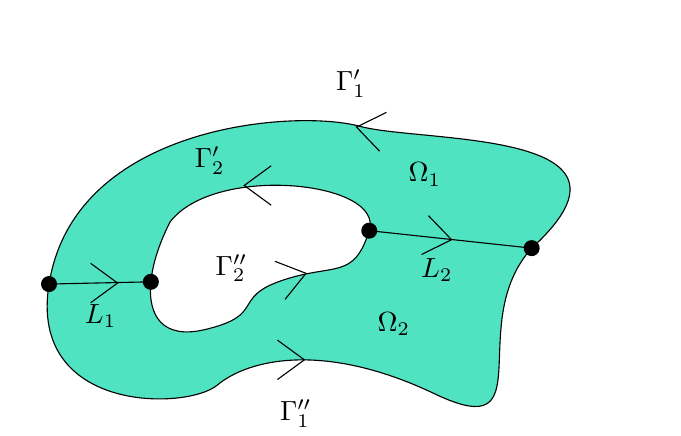
\begin{tikzpicture}[x=0.75pt,y=0.75pt,yscale=-1,xscale=1]
%uncomment if require: \path (0,334); %set diagram left start at 0, and has height of 334

%Curve Lines [id:da9623083499123468] 
\draw [fill={rgb, 255:red, 80; green, 227; blue, 194 }  ,fill opacity=1 ]   (388.49,126.68) .. controls (355.68,163.19) and (394.8,222.16) .. (341.79,196.89) .. controls (288.78,171.61) and (252.17,180.04) .. (237.03,192.68) .. controls (222.44,204.85) and (145.94,206.3) .. (155.96,143.99) .. controls (156.34,141.59) and (156.86,139.1) .. (157.51,136.51) .. controls (168.78,91.64) and (214.36,72.77) .. (253.43,67.17) .. controls (275.22,64.05) and (294.98,65.05) .. (305.65,67.97) .. controls (334.86,75.96) and (446.84,69.39) .. (392.18,123.2) .. controls (391.02,124.33) and (389.8,125.49) .. (388.49,126.68) -- cycle ;
%Curve Lines [id:da42174544578288087] 
\draw [fill={rgb, 255:red, 255; green, 255; blue, 255 }  ,fill opacity=1 ]   (214.31,114.04) .. controls (209.11,124.15) and (205.85,134.27) .. (205.02,142.91) .. controls (203.44,159.46) and (210.81,170.61) .. (230.72,166) .. controls (261.01,158.98) and (243.34,150.55) .. (268.58,142.13) .. controls (293.83,133.7) and (302.66,142.13) .. (310.24,118.26) .. controls (317.81,94.38) and (235.77,85.96) .. (214.31,114.04) -- cycle ;
%Straight Lines [id:da5237601037288719] 
\draw    (155.96,143.99) -- (205.02,142.91) ;
\draw [shift={(205.02,142.91)}, rotate = 358.73] [color={rgb, 255:red, 0; green, 0; blue, 0 }  ][fill={rgb, 255:red, 0; green, 0; blue, 0 }  ][line width=0.75]      (0, 0) circle [x radius= 3.35, y radius= 3.35]   ;
\draw [shift={(155.96,143.99)}, rotate = 358.73] [color={rgb, 255:red, 0; green, 0; blue, 0 }  ][fill={rgb, 255:red, 0; green, 0; blue, 0 }  ][line width=0.75]      (0, 0) circle [x radius= 3.35, y radius= 3.35]   ;
%Straight Lines [id:da27088478905554747] 
\draw    (310.24,118.26) -- (388.49,126.68) ;
\draw [shift={(388.49,126.68)}, rotate = 6.14] [color={rgb, 255:red, 0; green, 0; blue, 0 }  ][fill={rgb, 255:red, 0; green, 0; blue, 0 }  ][line width=0.75]      (0, 0) circle [x radius= 3.35, y radius= 3.35]   ;
\draw [shift={(310.24,118.26)}, rotate = 6.14] [color={rgb, 255:red, 0; green, 0; blue, 0 }  ][fill={rgb, 255:red, 0; green, 0; blue, 0 }  ][line width=0.75]      (0, 0) circle [x radius= 3.35, y radius= 3.35]   ;
\draw   (266,171) -- (279,180.5) -- (266,190) ;
\draw   (338.75,111.02) -- (349.9,122.63) -- (335.45,129.73) ;
\draw   (176,134) -- (189,143.5) -- (176,153) ;
\draw   (264.76,133.01) -- (279.78,138.82) -- (269.68,151.36) ;
\draw   (315.25,79.98) -- (304.1,68.37) -- (318.55,61.27) ;
\draw   (263,106) -- (250,96.5) -- (263,87) ;

% Text Node
\draw (172,152.4) node [anchor=north west][inner sep=0.75pt]    {$L_{1}$};
% Text Node
\draw (334,130.4) node [anchor=north west][inner sep=0.75pt]    {$L_{2}$};
% Text Node
\draw (266,198.4) node [anchor=north west][inner sep=0.75pt]    {$\Gamma ''_{1}$};
% Text Node
\draw (235,128.4) node [anchor=north west][inner sep=0.75pt]    {$\Gamma ''_{2}$};
% Text Node
\draw (225,76.4) node [anchor=north west][inner sep=0.75pt]    {$\Gamma '_{2}$};
% Text Node
\draw (293,39.4) node [anchor=north west][inner sep=0.75pt]    {$\Gamma '_{1}$};
% Text Node
\draw (313,156.4) node [anchor=north west][inner sep=0.75pt]    {$\Omega _{2}$};
% Text Node
\draw (328,84.4) node [anchor=north west][inner sep=0.75pt]    {$\Omega _{1}$};

\end{tikzpicture}
\end{center}

We set $\Gamma_1 = \Gamma'_1 + \Gamma''_1$ and $\Gamma_2 = \Gamma'_2 + \Gamma''_2$. 
The boundaries of $\Omega_1$ and $\Omega_2$ are simple closed curves that are oriented 
positively by 
\begin{align*}
    \partial\Omega_1 &= \Gamma'_1 + L_1 - \Gamma'_2 + L_2, \\
    \partial\Omega_2 &= \Gamma''_1 - L_2 - \Gamma''_2 - L_1. 
\end{align*}
By the Cauchy-Goursat Theorem, we have 
\[ \int_{\partial\Omega_1} f(z)\dd z = \int_{\partial\Omega_2} f(z)\dd z = 0, \]
which implies that 
\begin{align*}
    \int_{\Gamma'_1} f(z)\dd z &= \int_{\Gamma'_2 - L_1 - L_2} f(z) \dd z, \\
    \int_{\Gamma''_1} f(z) \dd z &= \int_{\Gamma''_2 + L_1 + L_2} f(z) \dd z.
\end{align*}
Finally, it follows that 
\[ \int_{\Gamma_1} f(z)\dd z = \int_{\Gamma'_1 + \Gamma''_1} f(z)\dd z = 
\int_{\Gamma'_2 + \Gamma''_2} f(z)\dd z = \int_{\Gamma_2} f(z)\dd z. \qedhere \]
\end{pf}

\begin{remark}
An important consequence of the Deformation Principle is that it allows us to compute contour 
integrals using simpler contours. For example, suppose that $\Omega \subseteq \C$ 
is a domain and $z_0 \in \Omega$. Consider a simple closed curve $\Gamma$ in $\Omega 
\setminus \{z_0\}$ whose interior contains $z_0$ and an analytic function $f$ on 
$\Omega \setminus \{z_0\}$. If $f$ is analytic on all of $\Omega$, then by the Cauchy-Goursat 
Theorem, we have 
\[ \int_\Gamma f(z)\dd z = 0. \]
However, if $f$ fails to be analytic at the point $z_0$, then one has to compute the 
integral directly, which can be quite complicated depending on the curve $\Gamma$. 
However, by the Deformation Principle, if $C_r = \{z \in \C : |z-z_0| = r\}$ is a 
circle centered at $z_0$ lying in the interior of $\Gamma$ with the 
same orientation as $\Gamma$, then 
\[ \int_\Gamma f(z)\dd z = \int_{C_r} f(z)\dd z. \]
\end{remark}

\begin{center}
\tikzset{every picture/.style={line width=0.75pt}} %set default line width to 0.75pt        

\begin{tikzpicture}[x=0.75pt,y=0.75pt,yscale=-1,xscale=1]
%uncomment if require: \path (0,334); %set diagram left start at 0, and has height of 334

%Curve Lines [id:da9623083499123468] 
\draw    (357.59,121.38) .. controls (326.73,162.34) and (363.53,228.5) .. (313.67,200.14) .. controls (263.82,171.79) and (229.39,181.24) .. (215.15,195.42) .. controls (201.43,209.07) and (129.49,210.7) .. (138.91,140.8) .. controls (139.27,138.11) and (139.75,135.31) .. (140.36,132.41) .. controls (149.92,87) and (185.74,65.32) .. (219.63,56.9) .. controls (221.8,56.36) and (223.96,55.88) .. (226.11,55.45) .. controls (227.6,55.15) and (229.1,54.87) .. (230.58,54.61) .. controls (251.06,51.11) and (269.65,52.24) .. (279.69,55.51) .. controls (307.16,64.48) and (412.47,57.11) .. (361.06,117.47) .. controls (359.97,118.74) and (358.82,120.04) .. (357.59,121.38) -- cycle ;
\draw   (246.16,171.1) -- (258.38,181.76) -- (246.16,192.42) ;
\draw   (289.65,68.99) -- (279.17,55.96) -- (292.76,48) ;
%Shape: Ellipse [id:dp9103895727660838] 
\draw   (196.73,121.5) .. controls (196.73,102.45) and (212.2,87) .. (231.28,87) .. controls (250.36,87) and (265.83,102.45) .. (265.83,121.5) .. controls (265.83,140.55) and (250.36,156) .. (231.28,156) .. controls (212.2,156) and (196.73,140.55) .. (196.73,121.5) -- cycle ;
\draw   (207.86,117.36) -- (197.43,125.95) -- (187,117.36) ;
\draw   (255.14,123.08) -- (265.57,114.5) -- (276,123.08) ;
%Shape: Ellipse [id:dp5132361117996211] 
\draw  [fill={rgb, 255:red, 0; green, 0; blue, 0 }  ,fill opacity=1 ] (228.74,121.5) .. controls (228.74,120.09) and (229.88,118.94) .. (231.28,118.94) .. controls (232.69,118.94) and (233.82,120.09) .. (233.82,121.5) .. controls (233.82,122.91) and (232.69,124.06) .. (231.28,124.06) .. controls (229.88,124.06) and (228.74,122.91) .. (228.74,121.5) -- cycle ;

% Text Node
\draw (368,134.4) node [anchor=north west][inner sep=0.75pt]    {$\Gamma $};
% Text Node
\draw (221.09,105) node [anchor=north west][inner sep=0.75pt]    {$z_{0}$};
% Text Node
\draw (183,142.4) node [anchor=north west][inner sep=0.75pt]    {$C_{r}$};

\end{tikzpicture}
\end{center}

One can also use the Deformation Principle to prove a more general form of Cauchy's Integral
Theorem. We leave this as an exercise. 

\begin{thm}[Cauchy's Integral Theorem for Jordan domains]
Let $\Omega \subseteq \C$ be a $k$-connected Jordan domain, and let $f$ be analytic 
on some domain $\Omega^+$ containing $\Omega$ and $\partial\Omega$. Then we have 
\[ \partial\Omega = \Gamma_1 + \cdots + \Gamma_k \]
for $k$ positively oriented Jordan curves $\Gamma_1, \dots, \Gamma_k \subseteq \Omega^+$, and 
\[ \int_{\partial\Omega} f(z)\dd z := \sum_{i=1}^k \int_{\Gamma_i} f(z)\dd z = 0. \]
\end{thm}

Recall that a Jordan domain is simply connected if it is $1$-connected. More generally, we have 
the following definition. 

\begin{defn}[Simply connected domain]
A domain $\Omega \subseteq \C$ is {\bf simply connected} if it has the property that 
if $\Gamma$ is any simply closed curve in $\Omega$, then the domain interior to 
$\Gamma$ is included in $\Omega$. 
\end{defn}

As usual, we can intuitively think of a simply connected domain as a domain which has "no holes". 

On a simply connected domain, we have another version of Cauchy's Integral Theorem. 

\begin{thm}[Cauchy's Integral Theorem for simply connected domains]
Suppose that $f$ is analytic on a simply connected domain $\Omega \subseteq \C$. Then for 
any closed curve $\Gamma$ in $\Omega$, we have 
\[ \int_\Gamma f(z)\dd z = 0. \]
Note that in the above statement, we do not assume that the closed curve $\Gamma$ is simple.
\end{thm}

\begin{remark}
As a consequence of the previous theorem, 
we have that if $f$ is analytic on a simply connected domain $\Omega \subseteq \C$, then
\begin{itemize}
    \item $f$ has an antiderivative throughout $\Omega$;
    \item $\int_\Gamma f(z)\dd z$ is independent of path for any contour $\Gamma$ in $\Omega$; and 
    \item $\int_\Gamma f(z)\dd z = 0$ for any loop $\Gamma$ in $\Omega$. 
\end{itemize}
\end{remark}

\begin{remark}
With the results we have seen so far, we give a general outline for computing 
integrals of complex-valued functions. 
\begin{enumerate}[(i)]
    \item For the definite integral of a complex-valued function of one real variable $f : 
    [a, b] \to \C$, proceed as in the real case and treat $i$ as a constant. 
    \item For the contour integral of an analytic function $f : \Omega \to \C$ over a 
    curve $\Gamma$ in a domain $\Omega \subseteq \C$ parametrized by $z : [a,b] \to \Gamma$: 
    \begin{itemize}
        \item If $\Gamma$ is a simple loop or a finite union of simple loops, then 
        the contour integral is zero. 
        \item If $\Gamma$ is not closed and we can find an antiderivative $F$ of $f$ 
        on $\Omega$, then 
        \[ \int_\Gamma f(z)\dd z = F(z(b)) - F(z(a)). \]
        \item Otherwise, directly compute the indefinite integral 
        \[ \int_\Gamma f(z)\dd z = \int_a^b f(z(t)) z'(t)\dd t. \]
        If necessary, use a simpler curve that can be deformed to $\Gamma$ 
        as in the Deformation Principle. 
    \end{itemize}
\end{enumerate}
\end{remark}

\newpage 
\section{Cauchy's Integral Formula and its consequences}

We now state an important theorem that will have many applications in this course. 

\begin{thm}[Cauchy's Integral Formula]
Let $f$ be analytic on a domain $\Omega \subseteq \C$, and let $\Gamma$ be a 
positively oriented simple closed curve inside $\Omega$ whose interior is also 
contained in $\Omega$. For any $z_0$ in the interior of $\Gamma$, we have 
\[ f(z_0) = \frac{1}{2\pi i} \int_\Gamma \frac{f(z)}{z-z_0}\dd z. \]
\end{thm}
\begin{pf}
Let $U$ be the interior of $\Gamma$. First, we note that since $z_0 \in U$ and 
$U$ is open, there exists $R > 0$ such that $D(z_0; R) \subseteq U \subseteq \Omega$. 
Choose $0 < r < R$ such that the circle $C_r = \{z \in \C : |z - z_0| = r\}$ 
is contained in $D(z_0; R)$, and hence also contained in $U$. Then, $C_r$ is a 
simple closed curve in $U$. Moreover, since $f(z)/(z-z_0)$ is analytic on 
$\Omega \setminus \{z_0\}$ and $z_0$ lies in the interior of $C_r$ 
(as it is the center of $C_r$), it follows from the Deformation Principle that 
\[ \int_\Gamma \frac{f(z)}{z-z_0}\dd z = \int_{C_r} \frac{f(z)}{z - z_0}\dd z, \]
where $C_r$ is positively oriented. Thus, it is enough to show that 
\[ \frac{1}{2\pi i} \int_{C_r} \frac{f(z)}{z-z_0}\dd z = f(z_0). \]
Note that we can write $f(z) = (f(z) - f(z_0)) + f(z_0)$ so that 
\[ \int_{C_r} \frac{f(z)}{z - z_0} \dd z = \int_{C_r} \frac{f(z) - f(z_0)}{z - z_0}\dd z 
+ \int_{C_r} \frac{f(z_0)}{z - z_0}\dd z. \]
Moreover, we have 
\[ \int_{C_r} \frac{f(z_0)}{z - z_0} \dd z = 2\pi i \cdot f(z_0). \]
Hence, it only remains to check that 
\[ I := \frac{1}{2\pi i} \int_{C_r} \frac{f(z) - f(z_0)}{z - z_0} \dd z = 0. \]
Indeed, since $f$ is analytic at $z_0$, it is continuous there. For any $\eps > 0$, 
there exists $\delta > 0$ such that 
\[ |f(z) - f(z_0)| < \eps \]
whenever $|z - z_0| < \delta$. Therefore, if $r < \delta$, then for any $z \in C_r$, 
we have 
\[ \left| \frac{f(z) - f(z_0)}{z - z_0} \right| = \frac{|f(z) - f(z_0)|}{|z-z_0|} 
= \frac{|f(z) - f(z_0)|}r < \frac{\eps}r. \]
In addition, $C_r$ has arclength $2\pi r$, so by the $ML$-inequality, we obtain 
\[ |I| < \frac{1}{2\pi} \cdot \frac{\eps}r \cdot 2\pi r = \eps. \]
Since $\eps > 0$ was arbitrary, it follows that $I = 0$. 
\end{pf}

\begin{remark}~
\begin{enumerate}[(i)]
    \item A nice consequence of Cauchy's Integral Formula is that one can determine all the 
    values of an analytic function in the interior of a simple loop $\Gamma$ 
    just by knowing its values on $\Gamma$. In particular, the behaviour of an 
    analytic function on a region is completely determined by its behaviour on the boundary. 
    \item Cauchy's Integral Formula can be used to compute contour integrals whose integrands 
    are of the form $f(z)/(z-z_0)$ where $f$ is analytic, since we have 
    \[ \int_\Gamma \frac{f(z)}{z-z_0} \dd z = 2\pi i \cdot f(z_0). \]
\end{enumerate}
\end{remark}

\begin{exmp}~
\begin{enumerate}[(1)]
    \item Consider the contour integral 
    \[ \int_\Gamma \frac{e^z + \sin z}z \dd z \]
    where $\Gamma$ is the circle $|z - 2| = 3$ traversed once in the counter-clockwise direction. 
    Observe that the integrand is of the form $f(z)/(z-z_0)$ where 
    $f(z) = e^z + \sin z$ and $z_0 = 0$. Moreover, $f$ is entire and $z_0$ lies in 
    $\Gamma$, so by Cauchy's Integral Formula, we have 
    \[ \int_\Gamma \frac{e^z + \sin z}z \dd z = 2\pi i \cdot f(0) = 2\pi i. \]
    \item Consider the contour integral 
    \[ \int_\Gamma \frac{\cos z}{z^2 - 4} \dd z \]
    where $\Gamma$ is a closed simple curve contained in $\Omega = \{z \in \C : x > -1\}$ 
    such that $z = 2$ lies in the interior of $\Gamma$. Note that the denominator of 
    the integrand $z^2 - 4$ vanishes at $z = \pm2$, but only $z = 2$ lies inside $\Gamma$. 
    Hence, we can write the integrand as $f(z)/(z-z_0)$ where 
    $f(z) = \cos z / (z+2)$ and $z_0 = 2$. Then $f(z)$ is analytic on the domain 
    $\Omega$ containing $\Gamma$ and $z_0$ lies inside $\Gamma$. It follows from 
    Cauchy's Integral Formula that 
    \[ \int_\Gamma \frac{\cos z}{z^2 - 4}\dd z = 2\pi i \cdot f(2) = 2\pi i \cdot 
    \frac{\cos 2}4 = \frac{\pi i \cos 2}2. \]
\end{enumerate}
\end{exmp}

As a consequence of Cauchy's Integral Formula, we obtain the following important result.

\begin{thm}
Let $f$ be analytic on a domain $\Omega \subseteq \C$. Then the derivatives 
of $f$ of every order exist and are analytic on $\Omega$. Moreover, 
for all $z_0 \in \Omega$, we have 
\[ f^{(n)}(z_0) = \frac{n!}{2\pi i} \int_\Gamma \frac{f(z)}{(z-z_0)^{n+1}}\dd z, \]
where $\Gamma$ is any positively oriented simple closed curve inside $\Omega$
such that the interior of $\Gamma$ contains $z_0$ and is contained in $\Omega$.
\end{thm}
\begin{pf}
We prove the formula for $n = 1$. As in the proof of Cauchy's Integral Formula, we have 
\[ \int_\Gamma \frac{f(z)}{(z-z_0)^2}\dd z = \int_{C_r} \frac{f(z)}{(z-z_0)^2} \dd z \]
for any circle $C_r = \{z \in \C : |z - z_0| = r\}$ centered at $z_0$ lying in the interior 
of $\Gamma$. We need to show that 
\[ \lim_{h\to0} \frac{f(z_0+h) - f(z_0)}{h} = \frac{1}{2\pi i} \int_{C_r} \frac{f(z)}{(z-z_0)^2}\dd z. \]
By Cauchy's Integral Formula, we know that 
\[ f(z_0) = \frac{1}{2\pi i} \int_{C_r} \frac{f(z)}{z-z_0}\dd z. \]
For $h$ sufficiently close to $0$, the point $z_0 + h$ also lies in $C_r$ so that 
\[ f(z_0 + h) = \frac{1}{2\pi i} \int_{C_r} \frac{f(z)}{z - (z_0 + h)} \dd z. \]
Moreover, we have 
\begin{align*}
    \frac{f(z_0 + h) - f(z_0)}h 
    &= \frac{1}{2\pi i} \int_{C_r} \frac1h \left( \frac{f(z)}{z - (z_0 + h)} - \frac{f(z)}{z-z_0} 
    \right) \dd z \\
    &= \frac{1}{2\pi i} \int_{C_r} \frac{f(z)}{(z-(z_0+h))(z-z_0)} \dd z. 
\end{align*}
Therefore, we obtain 
\begin{align*}
    \frac{f(z_0 + h) - f(z_0)}h - \frac{1}{2\pi i} \int_{C_r} \frac{f(z)}{(z-z_0)^2}\dd z 
    &= \frac{1}{2\pi i} \int_{C_r} \left[ \frac{f(z)}{(z-(z_0+h))(z-z_0)} - 
    \frac{f(z)}{(z-z_0)^2} \right] \dd z \\
    &= \frac{1}{2\pi i} \int_{C_r} \frac{f(z)h}{(z-(z_0+h))(z-z_0)^2}\dd z.
\end{align*}
Note that $C_r$ has arclength $2\pi r$ and $|z - z_0| = r$ since $z \in C_r$. 
It follows from the triangle inequality that 
\[ |z - (z_0 + h)| \geq |z - z_0| - |h| = r - |h| > 0. \]
whenever $|h| < r$. Thus, we have 
\[ \left| \frac{f(z)h}{(z-(z_0+h))(z-z_0)^2} \right| \leq \frac{|f(z)||h|}{(r-|h|)r^2}. \]
Finally, applying the $ML$-inequality gives 
\begin{align*}
    \left| \frac{f(z_0 + h) - f(z_0)}h - \frac{1}{2\pi i} \int_{C_r} \frac{f(z)}{(z-z_0)^2}\dd z 
    \right| 
    &\leq \frac{1}{2\pi} \cdot \frac{|f(z)||h|}{(r-|h|)r^2} \cdot 2\pi r 
    = \frac{|f(z)||h|}{(r-|h|)r},
\end{align*}
which tends to $0$ as $h$ approaches $0$. Thus, we conclude that 
\[ f'(z_0) = \frac{1}{2\pi i} \int_{C_r} \frac{f(z)}{(z-z_0)^2}\dd z. \]
One can repeat this procedure for the general case; we leave the details as an exercise. 
\end{pf}

\begin{remark}
Due to Theorem 19.4, we see that for an analytic function, the existence of its 
derivative on an open set ensures that its derivatives exist up to any order. 
In particular, this implies that the real and imaginary parts of analytic functions are smooth.
\end{remark}

\newpage 
\section{Complex analogues of properties of harmonic functions}

In the previous lecture, we finally proved that the real and imaginary parts of an analytic 
function are smooth, implying that they are harmonic since they satisfy the 
Cauchy-Riemann equations. Given this fact, several theorems we have seen for 
harmonic functions have counterparts for complex analytic functions. 

First, we consider the complex analogues of the Circumferential and Solid MVTs. 

\begin{thm}
Let $f$ be analytic on a domain $\Omega \subseteq \C$ which contains the closed disc $\overline{D}(z_0; r)$. 
\begin{enumerate}[(i)]
    \item (Circumferential MVT) Then $f(z_0)$ is the arithmetic mean of the values that $f$ 
    assumes on the circumference of the disc; that is, we have 
    \[ f(z_0) = \frac{1}{2\pi} \int_0^{2\pi} f(z_0 + re^{i\theta})\dd \theta. \]
    \item (Solid MVT) We have 
    \[ f(z_0) = \frac{1}{\pi r^2} \iint_{D(z_0; r)} f(z)\dd x \dd y. \]
\end{enumerate}
\end{thm}
\begin{pf}
Let $u$ and $v$ be the real and imaginary parts of $f$ respectively so that $f = u + iv$. 
Since $f$ is analytic on $\Omega$, we know that $u$ and $v$ are harmonic on $\Omega$. 
\begin{enumerate}[(i)]
    \item By the Circumferential MVT for harmonic functions (Theorem 6.5), we have 
    \begin{align*} f(z_0) = u(z_0) + iv(z_0) 
    &= \frac{1}{2\pi} \int_0^{2\pi} u(z_0 + re^{i\theta}) \dd \theta + i 
    \cdot \frac{1}{2\pi} \int_0^{2\pi} v(z_0 + re^{i\theta}) \dd \theta \\
    &= \frac{1}{2\pi} \int_0^{2\pi} f(z_0 + re^{i\theta})\dd \theta. \end{align*}
    \item By the Solid MVT for harmonic functions (Theorem 6.9), we similarly obtain 
    \begin{align*} f(z_0) = u(z_0) + iv(z_0) 
    &= \frac{1}{\pi r^2} \iint_{D(z_0; r)} u(z)\dd x \dd y + i 
    \cdot \frac{1}{\pi r^2} \iint_{D(z_0; r)} v(z)\dd x \dd y \\
    &= \frac{1}{\pi r^2} \iint_{D(z_0; r)} f(z)\dd x \dd y. \qedhere \end{align*} 
    \end{enumerate}
\end{pf}

We now turn to the complex analogue of the Maximum Principle for harmonic functions (which 
was the main topic of Lecture 7). Recall that the Maximum Principle tells us that 
a non-constant function harmonic function cannot assume a maximum on a domain. 
For a complex-valued function, it does not make sense to consider its maximum value 
since there is no ordering on the complex numbers. Nonetheless, we can consider its 
maximum modulus. 

\begin{defn}[Maximum modulus]
Let $\Omega \subseteq \C$ be a domain and let $f$ be a complex-valued function on $\C$. 
We say that {\bf $f$ attains a maximum modulus at $z_0$ in $\Omega$} if 
\[ |f(z)| \leq |f(z_0)| \]
for all $z \in \Omega$. 
\end{defn}

\begin{remark}
Geometrically, if $f$ attains a maximum modulus at $z_0$ in $\Omega$, then 
$f(z_0)$ is the furthest point from the origin in $f(\Omega)$.
\end{remark}

\begin{thm}[Strong Maximum Modulus Principle]
Let $f$ be an analytic function on a domain $\Omega \subseteq \C$ and suppose that 
it attains a maximum modulus in $\Omega$. Then $f$ is constant.
\end{thm}
\begin{pf}
Suppose that $f$ attains a maximum modulus at $z_0 \in \Omega$ and set $c_0 = |f(z_0)|$. 
Choose $c \in R^{>0}$ such that $c > c_0$ and $g(z) 
= f(z) + cf(z_0)$ is such that $g(\Omega) \subseteq D^*_\tau = \C \setminus \{re^{i\tau} : r \geq 0\}$
for some $\tau \in \R$. This is certainly possible since $g$ is simply $f$ translated by 
$cf(z_0)$. 

The composition $L_\tau(g(z))$ is then defined and analytic on $\Omega$, which implies that its 
real part $\ln|g(z)|$ is harmonic on $\Omega$. Moreover, $\ln|g(z)|$ attains its maximum on 
$z_0$. Indeed, for all $z \in \Omega$, we have 
\[ |g(z)| \leq |f(z)| + c|f(z_0)| \leq |f(z_0)| + c|f(z_0)| = |g(z_0)|. \]
Since $\ln|\cdot|$ is monotone increasing, it follows that 
\[ \ln|g(z)| \leq \ln|g(z_0)| \]
for all $z \in \Omega$, so $\ln|g(z)|$ attains its maximum at $z_0$. This can only happen if 
$\ln|g(z)|$ is constant by the harmonicity of $\ln|g(z)|$ in $\Omega$. 
By part (c) of Question 1 on Assignment 5, this in turn implies that $|g(z)|$ and $g(z)$ are 
constant in $\Omega$, and hence so is $f$. 
\end{pf}

\begin{remark}
The Strong Maximum Modulus Principle equivalently states that a non-constant analytic 
function in a domain $\Omega \subseteq \C$ does not attain its maximum modulus at any 
point in $\Omega$. 
\end{remark}

\begin{thm}[Minimum Modulus Principle]
Let $f$ be a non-constant analytic function on the domain $\Omega$ with $f(z) \neq 0$
for all $z \in \C$. Then $f$ does not attain its minimum modulus at any point in $\Omega$. 
\end{thm}
\begin{pf}
Apply the Strong Maximum Modulus Principle to $1/f(z)$. 
\end{pf}

\begin{exmp}
Consider the function $f(z) = (z+1)^2$, which is entire. Let $\Omega$ be the 
interior of the triangle with vertices $z = 0$, $z = 2$, and $z = i$. Note that 
\[ |f(z)| = |(x+1) + iy|^2 = (x+1)^2 + y^2, \]
which has maximum value $9$ at $z = 2$ and minimum value $1$ at $z = 0$ on $\overline\Omega$. 
Both the maximum and minimum occur on $\partial\Omega$, confirming the Maximum and 
Minimum Modulus Principles. 
\end{exmp}

The fact that the maximum of $|f(z)|$ occurs on $\partial\Omega$ in Example 20.7 is due to the following 
theorem. 

\begin{thm}[Weak Maximum Modulus Principle]
Let $\Omega \subseteq \C$ be a bounded domain such that $f$ is continuous on $\overline\Omega$ 
and analytic on $\Omega$. Then $f$ is either constant or attains its maximum modulus over 
$\overline\Omega$ on $\partial\Omega$ only. 
\end{thm}
\begin{pf}
Since $|f(z)|$ is continuous on the compact set $\overline\Omega$, it has a maximum on 
$\overline\Omega$ by the Extreme Value Theorem, which can only be attained on $\partial\Omega$
by the Strong Maximum Modulus Principle if $f$ is a non-constant function. 
\end{pf}

Recall that harmonic functions are completely and uniquely determined by their boundary behaviour 
(by Theorem 7.7). The same is also true of analytic functions. 

\begin{thm}
Let $f$ and $g$ be analytic functions on a domain $\Omega \subseteq \C$, and let 
$\Gamma$ be a simple closed curve whose interior lies inside $\Omega$. If $f$ and $g$ 
are equal on $\Gamma$, then they are also equal on the interior of $\Gamma$.
\end{thm}
\begin{pf}
Let $\Omega'$ be the interior of $\Gamma$. Since $\Gamma$ is simple and closed, we see that 
$\Omega'$ is a domain. Moreover, since $\overline{\Omega'} \subseteq \Omega$, we have that 
$f$ and $g$ are analytic on $\overline{\Omega'}$, so they are continuous on 
$\partial\Omega'$ and analytic on $\Omega'$. Their real and imaginary parts are then continuous 
and equal on $\partial\Omega'$ and harmonic on $\Omega'$, implying that they are also equal on 
$\Omega'$. 
\end{pf}

\begin{remark}
In fact, $f$ and $g$ are equal on $\Omega$ since they agree on an open set. This result 
is known as the Identity Theorem, which we will prove later. 
\end{remark}

We now consider the complex counterpart of Liouville's Theorem (Theorem 8.2), which states that 
bounded entire harmonic functions are constant. 

\begin{thm}[Liouville's Theorem]
A bounded entire complex function is constant.
\end{thm}
\begin{pf}
If $f = u+iv$ is entire, then $u$ and $v$ are entire harmonic functions. Moreover, for all $z \in 
\C$, we have 
\[ |u(z)| \leq |u(z) + iv(z)| = |f(z)|, \]
and similarly $|v(z)| \leq |f(z)|$. Since $f$ is bounded, so are $u$ and $v$. By Liouville's 
Theorem for harmonic functions, $u$ and $v$ are constant. Consequently, $f$ is constant. 
\end{pf}

Finally, as an application of Liouville's Theorem, we prove the Fundamental Theorem of Algebra. 

\begin{thm}[Fundamental Theorem of Algebra]
Let $p(z) = a_0 + a_1z + \cdots + a_n z^n$ be a polynomial of degree $n \geq 1$ 
with complex coefficients. Then $p(z)$ has a root in $\C$. 
\end{thm}
\begin{pf}
Suppose to the contrary that $p(z)$ has no roots in $\C$ so that $p(z) \neq 0$ for all 
$z \in \C$. Then 
\[ f(z) = \frac1{p(z)} \] 
is entire since it is a rational function whose denominator never vanishes. We show that 
$f$ is bounded. First, note that $p(z) = (a_n + w)z^n$ where 
\[ w = \frac{a_{n-1}}z + \frac{a_{n-2}}{z^2} + \cdots + \frac{a_0}{z^n}. \]
We claim that there exists $R > 1$ such that 
\[ \frac{|a_i|}{|z|^{n-i}} < \frac{|a_n|}{2n} \]
for all $0 \leq i \leq n-1$ whenever $|z| > R$. Indeed, let 
\[ s = \max_{0\leq i \leq n-1} |a_i| \]
and choose $R > 1$ such that 
\[ \frac sR < \frac{|a_n|}{2n}. \]
Then $|z|^{n-i} > R^{n-i} \geq R$ for all $|z| > R$ since $R > 1$, which implies that 
\[ \frac{|a_i|}{|z|^{n-i}} < \frac sR < \frac{|a_n|}{2n} \]
for all $0 \leq i \leq n-1$. Moreover, by the triangle inequality, we have 
\[ |w| \leq \frac{|a_{n-1}|}{|z|} + \frac{|a_{n-2}|}{|z|^2} + \cdots + \frac{|a_0|}{|z|^n} 
< n \cdot \frac{|a_n|}{2n} = \frac{|a_n|}2, \]
and so $|a_n - w| \geq ||a_n| - |w|| > |a_n|/2$. Hence, when $|z| > R$, we obtain 
\[ |p(z)| = |a_n + w||z|^n > \frac{|a_n|}2 \cdot R^n = \frac{|a_n|R^n}2, \]
so it follows that 
\[ |f(z)| = \frac{1}{|p(z)|} < \frac{2}{|a_n|R^n}. \]
Therefore, $f$ is bounded on $|z| > R$. Moreover, since $f$ is continuous, it is also bounded on the 
closed disc $|z| \leq R$ by the Extreme Value Theorem. Thus, $f$ is bounded on $\C$. 

Finally, we have by Liouville's Theorem that $f$ is constant. But this implies that $p$ 
is constant, which is a contradiction as $p$ is a polynomial of degree $n \geq 1$.
\end{pf}

\newpage 
\section{More consequences of Theorem 19.4}

Recall that Theorem 19.4 states that if $f$ is analytic on a domain $\Omega \subseteq \C$, then 
its derivatives of every order exist and are analytic on $\Omega$. Moreover, for all 
$z_0 \in \Omega$ and every integer $n \geq 0$, we have 
\[ f^{(n)}(z_0) = \frac{n!}{2\pi i} \int_\Gamma \frac{f(z)}{(z-z_0)^{n+1}}\dd z \tag{$\star$}, \] 
where $\Gamma$ is any positively oriented simple closed curve inside $\Omega$ whose 
interior contains $z_0$ and is contained in $\Omega$. The formulae given by 
$(\star)$ are known as the {\bf Cauchy Integral Formulae}. 

As a consequence of Theorem 19.4, we saw that the real and imaginary parts of an analytic function 
are smooth and hence harmonic. In Lecture 20, we used this fact to show that many 
of the properties of harmonic functions have analogues for complex analytic functions. 

In this lecture, we will explore three more consequences of Theorem 19.4. 
\begin{itemize}
    \item (Morera's Theorem) This theorem can be viewed as the converse of the Cauchy-Goursat Theorem. 
    It states that if a continuous function on a domain $\Omega \subseteq \C$ has the 
    path independence property, then it is analytic on $\Omega$. 
    \item The Cauchy Integral Formulae in $(\star)$ can be used to compute contour integrals 
    whose integrands are of the form $f(z)/(z-z_0)^{n+1}$ since we have 
    \[ \int_\Gamma \frac{f(z)}{(z-z_0)^{n+1}}\dd z = \frac{2\pi i}{n!} f^{(n)}(z_0). \]
    \item (Cauchy's inequality) The Cauchy Integral Formulae can also be used to find 
    local upper bounds for the derivatives of an analytic function up to any order. 
\end{itemize}
Recall that the Cauchy-Goursat Theorem tells us that if a function is analytic on and 
inside a simply closed curve $\Gamma$, then 
\[ \int_\Gamma f(z) \dd z = 0. \]
It turns out that the converse is true; this relies on the fact that the derivatives of 
an analytic function exist and are analytic up to any order. 

\begin{thm}[Morera's Theorem]
Let $f$ be a continuous complex-valued function on a domain $\Omega \subseteq \C$. If 
\[ \int_\Gamma f(z)\dd z = 0 \]
for every closed curve $\Gamma$ in $\Omega$, then $f$ is analytic on $\Omega$. 
\end{thm}
\begin{pf}
First, note that if we have
\[ \int_\Gamma f(z)\dd z = 0 \]
for every closed curve $\Gamma$ in $\Omega$, then $f$ has an antiderivative $F$ in $\Omega$ 
by independence of path. In particular, we have $F'(z) = f(z)$ for all $z \in \Omega$, so 
$F$ is analytic on $\Omega$. Since the derivatives of an analytic function exist and 
are analytic up to any order, we see that $f = F'$ is also analytic on $\Omega$. 
\end{pf}

We mentioned that the Cauchy Integral Formulae can be used to compute contour 
integrals whose integrands are of the form $f(z)/(z-z_0)^{n+1}$, since we have 
\[ \int_\Gamma \frac{f(z)}{(z-z_0)^{n+1}}\,{\rm d}z = \frac{2\pi i}{n!} f^{(n)}(z_0) \]
as long as $z_0$ lies in the interior of $\Gamma$. We have already seen this in
case that $n = 0$, so we will look at some examples where $n \geq 1$. 

\begin{exmp}
Consider the contour integral 
\[ \int_\Gamma \frac{5z^2+2z+1}{(z-i)^3}\dd z \]
where $\Gamma$ is the circle $|z| = 2$ traversed once in the counter-clockwise direction. 
Then the integrand is of the form $f(z)/(z-z_0)^{n+1}$ where $f(z) = 5z^2+2z+1$, 
$z_0 = i$, and $n = 2$. Moreover, $f$ is entire and $z_0$ lies inside $\Gamma$. 
Therefore, by the Cauchy Integral Formulae, we have 
\[ \int_\Gamma \frac{5z^2+2z+1}{(z-i)^3}\dd z = \frac{2\pi i}{2!} f''(i) = \frac{2\pi i}2(10) = 10\pi i. \]
\end{exmp}

\begin{exmp}
Consider the contour integral 
\[ \int_\Gamma \frac{2z+1}{z(z-1)^2}\dd z \]
where $\Gamma$ is the sketched figure-eight curve below. 

\begin{center}

\tikzset{every picture/.style={line width=0.75pt}} %set default line width to 0.75pt        

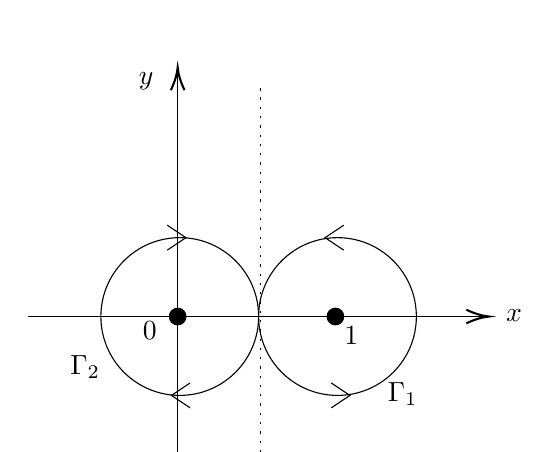
\begin{tikzpicture}[x=0.75pt,y=0.75pt,yscale=-1,xscale=1]
%uncomment if require: \path (0,334); %set diagram left start at 0, and has height of 334

%Straight Lines [id:da04186956827712951] 
\draw    (148,150) -- (368,150) ;
\draw [shift={(370,150)}, rotate = 180] [color={rgb, 255:red, 0; green, 0; blue, 0 }  ][line width=0.75]    (10.93,-3.29) .. controls (6.95,-1.4) and (3.31,-0.3) .. (0,0) .. controls (3.31,0.3) and (6.95,1.4) .. (10.93,3.29)   ;
%Straight Lines [id:da06567403778816683] 
\draw    (220,220) -- (220,32) ;
\draw [shift={(220,30)}, rotate = 450] [color={rgb, 255:red, 0; green, 0; blue, 0 }  ][line width=0.75]    (10.93,-3.29) .. controls (6.95,-1.4) and (3.31,-0.3) .. (0,0) .. controls (3.31,0.3) and (6.95,1.4) .. (10.93,3.29)   ;
%Straight Lines [id:da9169000458332186] 
\draw  [dash pattern={on 0.84pt off 2.51pt}]  (260,40) -- (260,220) ;
%Shape: Circle [id:dp06905198372773125] 
\draw  [fill={rgb, 255:red, 0; green, 0; blue, 0 }  ,fill opacity=1 ] (216,150) .. controls (216,147.79) and (217.79,146) .. (220,146) .. controls (222.21,146) and (224,147.79) .. (224,150) .. controls (224,152.21) and (222.21,154) .. (220,154) .. controls (217.79,154) and (216,152.21) .. (216,150) -- cycle ;
%Shape: Circle [id:dp036569142221264395] 
\draw  [fill={rgb, 255:red, 0; green, 0; blue, 0 }  ,fill opacity=1 ] (292,150) .. controls (292,147.79) and (293.79,146) .. (296,146) .. controls (298.21,146) and (300,147.79) .. (300,150) .. controls (300,152.21) and (298.21,154) .. (296,154) .. controls (293.79,154) and (292,152.21) .. (292,150) -- cycle ;
%Shape: Circle [id:dp839220973755354] 
\draw   (183,150) .. controls (183,129.01) and (200.01,112) .. (221,112) .. controls (241.99,112) and (259,129.01) .. (259,150) .. controls (259,170.99) and (241.99,188) .. (221,188) .. controls (200.01,188) and (183,170.99) .. (183,150) -- cycle ;
%Shape: Circle [id:dp45878709870692913] 
\draw   (259,150) .. controls (259,129.01) and (276.01,112) .. (297,112) .. controls (317.99,112) and (335,129.01) .. (335,150) .. controls (335,170.99) and (317.99,188) .. (297,188) .. controls (276.01,188) and (259,170.99) .. (259,150) -- cycle ;
\draw   (294,182) -- (303,188) -- (294,194) ;
\draw   (215,106) -- (224,112) -- (215,118) ;
\draw   (300,118) -- (291,112) -- (300,106) ;
\draw   (226,194) -- (217,188) -- (226,182) ;

% Text Node
\draw (202,151.4) node [anchor=north west][inner sep=0.75pt]    {$0$};
% Text Node
\draw (299,153.4) node [anchor=north west][inner sep=0.75pt]    {$1$};
% Text Node
\draw (377,145.4) node [anchor=north west][inner sep=0.75pt]    {$x$};
% Text Node
\draw (200,31.4) node [anchor=north west][inner sep=0.75pt]    {$y$};
% Text Node
\draw (320,180.4) node [anchor=north west][inner sep=0.75pt]    {$\Gamma _{1}$};
% Text Node
\draw (167,167.4) node [anchor=north west][inner sep=0.75pt]    {$\Gamma _{2}$};
\end{tikzpicture}
\end{center}
Note that integration along $\Gamma$ is equivalent to integrating once around the 
positively oriented right loop $\Gamma_1$ and once around the negatively oriented left loop 
$\Gamma_2$. That is, we have 
\[ \int_\Gamma \frac{2z+1}{z(z-1)^2}\dd z = \int_{\Gamma_1} \frac{(2z+1)/z}{(z-1)^2}\dd z 
+ \int_{\Gamma_2} \frac{(2z+1)/(z-1)^2}{z}\dd z. \]
Moreover, the integrand $(2z+1)/[z(z-1)^2]$ is analytic everywhere except at $z = 0$ and 
$z = 1$, with $z = 1$ in the interior of $\Gamma_1$ and $z = 0$ in the interior of $\Gamma_2$. 

We first focus on computing 
\[ \int_{\Gamma_1} \frac{(2z+1)/z}{(z-1)^2}\dd z. \]
The integrand is of the form $f(z)/(z-z_0)^{n+1}$ where $f(z) = (2z+1)/z$, $z_0 = 1$, and 
$n = 1$. Then $f$ is analytic on a domain containing $\Gamma_1$ (such as 
$\Omega = \{z \in \C : x > 0\})$ and $z_0$ lies inside $\Gamma_1$. Since $\Gamma_1$ is 
positively oriented, the Cauchy Integral Formulae implies that 
\[ \int_{\Gamma_1} \frac{(2z+1)/z}{(z-1)^2}\dd z = \frac{2\pi i}{1!} f'(1) = 
2\pi i \cdot (-1) = -2\pi i. \]
Now, we look at 
\[ \int_{\Gamma_2} \frac{(2z+1)/(z-1)^2}{z}\dd z. \]
Observe that the integrand is of the form $f(z)/(z-z_0)^{n+1}$ where 
$f(z) = (2z+1)/(z-1)^2$, $z_0 = 0$, and $n = 0$. Note that $f$ is analytic on a domain 
containing $\Gamma_2$ (such as $\Omega' = \{z \in \C : x < 1\}$ and $z_0$ lies in $\Gamma_2$. 
Since $\Gamma_2$ is negatively oriented, it follows from the Cauchy Integral Formulae that 
\[ \int_{\Gamma_2} \frac{(2z+1)/(z-1)^2}{z}\dd z = - \frac{2\pi i}{0!} f(0) = 
-2\pi i \cdot 1 = -2\pi i. \]
Putting these together, we obtain 
\[ \int_\Gamma \frac{2z+1}{z(z-1)^2}\dd z = -2\pi i - 2\pi i = -4\pi i. \]
\end{exmp}

We end our discussion on complex integration with a technical result that illustrates to 
what extent analyticity puts restrictions on the behaviour of a function.

\begin{thm}[Cauchy's inequality]
Let $f$ be analytic on the closed disc $\overline{D}(z_0; r)$, and let $M(z_0; r)$ 
be its maximum modulus on the boundary circle $C(z_0; r) = \{z \in \C : |z - z_0| = r\}$. 
(The maximum modulus $M(z_0; r)$ exists and is attained on $C(z_0; r)$ by the Maximum 
Modulus Principle.) Then we have 
\[ |f^{(n)}(z_0)| \leq \frac{n!M(z_0; r)}{r^n}. \]
\end{thm}
\begin{pf}
By the Cauchy Integral Formulae, we have 
\[ f^{(n)}(z_0) = \frac{n!}{2\pi i} \int_{C(z_0; r)} \frac{f(z)}{(z-z_0)^{n+1}}\dd z. \]
Moreover, the circle $C(z_0; r)$ has arclength $2\pi r$ and 
\[ \left| \frac{f(z)}{(z-z_0)^{n+1}} \right| = \frac{|f(z)|}{|z-z_0|^{n+1}}
= \frac{|f(z)|}{r^{n+1}} \leq \frac{M(z_0; r)}{r^{n+1}} \]
for all $z \in C(z_0; r)$. Hence, by the $ML$-inequality, we obtain 
\[ |f^{(n)}(z_0)| \leq \frac{n!}{2\pi} \cdot \frac{M(z_0; r)}{r^{n+1}} \cdot 2\pi r = 
\frac{n!M(z_0; r)}{r^n}. \qedhere \]
\end{pf}

\begin{remark}
One can use Cauchy's inequality to give an alternative proof of Liouville's Theorem. 
Indeed, let $f$ be a bounded entire function. Then there exists $M > 0$ such that 
\[ |f(z)| \leq M \] 
for all $z \in \C$. Then for any circle $C(z_0; r) = \{z \in \C : |z - z_0| = r\}$, we have 
\[ |f'(z_0)| \leq \frac{M(z_0; r)}r \leq \frac{M}r \]
by Cauchy's inequality with $n = 1$. Since $M/r \to 0$ as $r \to \infty$, it follows that 
$|f'(z_0)| = 0$, so $f'(z_0) = 0$ for all $z_0 \in \C$. Thus, $f$ is constant. 
\end{remark}

\newpage 
\section{Complex sequences and series}

We now begin looking at sequences and series of complex numbers and functions. 
In this lecture, we will review the complex analogues of the main definitions and results of 
sequences and series of real numbers.

\begin{defn}
A {\bf sequence} $\{z_n\}_{n=1}^\infty$ of complex numbers is a set of complex numbers 
indexed by the positive integers (or the natural numbers). A sequence $\{z_n\}_{n=1}^\infty$ 
is said to be {\bf bounded} if there exists a real number $M > 0$ such that 
$|z_n| < M$ for all $n \in \Z^+$. 
\end{defn}

\begin{exmp}~
\begin{enumerate}[(1)]
    \item The sequences $\{i^n\}_{n=0}^\infty$ and $\{i^n/n\}_{n=1}^\infty$ are both bounded. 
    \item The sequence $\{1+in\}_{n=0}^\infty$ is not bounded. 
\end{enumerate}
\end{exmp}

\begin{defn}
A sequence $\{z_n\}_{n=1}^\infty$ is said to {\bf converge} to $z$ if for every $\eps > 0$, 
there exists an integer $n_0$ such for all $n > n_0$, we have $|z_n - z| < \eps$, 
in which case we write $\lim_{n\to\infty} z_n = z$. If $\{z_n\}_{n=1}^\infty$ 
does not converge to any complex number, then the sequence is said to {\bf diverge}. 
\end{defn}

\begin{remark}
It follows immediately from the definition that convergent sequences are bounded. 
Moreover, a sequence $\{z_n\}_{n=1}^\infty$ diverges if and only if for any complex number $z$, 
there exists $\eps_0 > 0$ such that for all $N \in \Z^+$, we have $|z_n - z| \geq \eps_0$ for some 
$n \geq N$. 
\end{remark}

\begin{exmp}~
\begin{enumerate}[(1)]
    \item The sequence $\{i^n/n\}_{n=1}^\infty$ converges since for any $\eps > 0$, 
    we can choose $n_0 \in \Z^+$ such that $1/n_0 < \eps$, in which case we have 
    \[ |i^n/n| = 1/n < 1/n_0 < \eps \]
    for all $n > n_0$. 
    \item The sequence $\{1+in\}_{n=0}^\infty$ diverges since it is not bounded. 
\end{enumerate}
\end{exmp}

In the case where the sequence has a general term $z_n = x_n + iy_n$ where $x_n, y_n \in \R$ for all 
$n \in \Z^+$, one can determine whether it converges or diverges by looking at its real and imaginary 
parts. 

\begin{thm}
The sequence $\{z_n = x_n + iy_n\}_{n=1}^\infty$ converges to $z = x+iy$ if and only if 
$\lim_{n\to\infty} x_n = x$ and $\lim_{n\to\infty} y_n = y$. 
\end{thm}
\begin{pf}
Exercise. 
\end{pf}

\begin{exmp}~
\begin{enumerate}[(1)]
    \item The sequence $\{1/n^2 + 2i/n^3\}_{n=1}^\infty$ converges to $0$. Indeed, the general 
    term of the sequence is $z_n = x_n + iy_n$ where $x_n = 1/n^2$ and $y_n = 2/n^3$, and we have 
    $\lim_{n\to\infty} 1/n^2 = \lim_{n\to\infty} 2/n^3 = 0$. 
    \item The sequence $\{(3-n^2i)/n\}_{n=1}^\infty$ diverges since the imaginary part of 
    $(3-n^2i)/n$ is $-n$, and $\{-n\}_{n=1}^\infty$ diverges. 
    \item The sequence $\{i^n\}_{n=0}^\infty$ diverges since $i^n = x_n + iy_n$ where we have 
    $\{x_n\}_{n=0}^\infty = \{1, 0, -1, 0, 1, 0, \dots\}$ and 
    $\{y_n\}_{n=0}^\infty = \{0, 1, 0, -1, 0, 1, \dots\}$, and both of these sequences are divergent. 
\end{enumerate}
\end{exmp}

\begin{defn}
An {\bf infinite series} $\sum_{n=1}^\infty z_n$ of a complex sequence $\{z_n\}_{n=1}^\infty$ 
is said to {\bf converge} to a sum $S$ if and only if the {\bf sequence of partial sums} 
\[ S_n := z_1 + \cdots + z_N \] 
converges to $S$. Otherwise, we say that $\sum_{n=1}^\infty z_n$ is {\bf divergent}. 
\end{defn}

\begin{thm}
Let $\sum_{n=1}^\infty z_n$ be a complex series with $z_n = x_n + iy_n$. 
\begin{enumerate}[(1)]
    \item We have $\sum_{i=1}^\infty z_n = x + iy$ if and only if $\sum_{n=1}^\infty x_n = x$ and 
    $\sum_{n=1}^\infty y_n = y$. 
    \item (Divergence Test) If $\lim_{n\to\infty} z_n \neq 0$, then $\sum_{n=1}^\infty z_n$ diverges. 
    \item (Absolute convergence) If $\sum_{n=1}^\infty |z_n|$ is convergent, then 
    $\sum_{n=1}^\infty z_n$ is convergent. 
\end{enumerate}
\end{thm}
\begin{pf}
Exercise. 
\end{pf}

\begin{exmp}~
\begin{enumerate}[(1)]
    \item Recall the $p$-series $\sum_{n=1}^\infty n^p$, which converges if and only if $p < -1$. 
    Then by part (1) of Theorem 22.9, we see that 
    \begin{itemize}
        \item $\sum_{n=1}^\infty (1/n^2 - 2i/n^3)$ converges since $\sum_{n=1}^\infty 1/n^2$ and 
        $\sum_{n=1}^\infty -2/n^3$ both converge, and 
        \item $\sum_{n=1}^\infty (1/n^2 - 2i/n)$ diverges since $\sum_{n=1}^\infty -2/n$ diverges. 
    \end{itemize}
    \item Observe that $\sum_{n=1}^\infty (n-i)/n$ diverges by the Divergence Test since 
    \[ \frac{n-i}n = 1 - \frac in \xrightarrow[]{n\to\infty} 1 \neq 0. \]
    \item (Complex geometric series) Fix $b \in \C$. We claim that 
    \[ \sum_{n=0}^\infty b^n \]
    converges if and only if $|b| < 1$. Indeed, recall the real geometric series $\sum_{n=0}^\infty a^n$ 
    with $a \in \R$, which converges if and only if $|a| < 1$. Hence, $\sum_{n=0}^\infty |b|^n$ 
    converges if and only if $|b| < 1$. 
    \begin{itemize}
        \item If $|b| < 1$, then $\sum_{n=0}^\infty |b^n| = \sum_{n=0}^\infty |b|^n$ converges
        by what we just noted, 
        and hence $\sum_{n=0}^\infty b^n$ converges by absolute convergence. 
        \item If $|b| \geq 1$, then we see that $b^n \nrightarrow 0$ as $n \to \infty$ (since 
        $|b|^n \nrightarrow 0$ as $n \to \infty$), so $\sum_{n=0}^\infty b^n$ diverges by the 
        Divergence Test. 
    \end{itemize}
\end{enumerate}
\end{exmp}

We give two more familiar tests for convergence.

\begin{thm}
Let $\sum_{n=1}^\infty z_n$ be a complex series.
\begin{enumerate}[(1)]
    \item (Ratio Test) Suppose that $\lim_{n\to\infty} |z_{n+1}/z_n| = L$. 
    \begin{itemize}
        \item If $L < 1$, then $\sum_{n=1}^\infty z_n$ converges. 
        \item If $L > 1$, then $\sum_{n=1}^\infty z_n$ diverges. 
        \item If $L = 1$, then the test is inconclusive. 
    \end{itemize}
    \item (Comparison Test) Suppose there exists $n_0 \in \Z^+$ and a real sequence $\{r_n\}_{n=1}^\infty$ 
    such that 
    \[ |z_n| \leq r_n \]
    for all $n \geq n_0$. If $\sum_{n=1}^\infty r_n$ converges, then $\sum_{n=1}^\infty z_n$ converges. 
\end{enumerate}
\end{thm}
\begin{pf}~
\begin{enumerate}[(1)]
    \item First, suppose that $L < 1$. Then 
    \[ \lim_{n\to\infty} \frac{|z_{n+1}|}{|z_n|} = L, \]
    so by the real Ratio Test, we see that $\sum_{n=1}^\infty |z_n|$ is convergent. 
    By absolute convergence, $\sum_{n=1}^\infty z_n$ is convergent. 
    
    Suppose now that $L > 1$. Then for sufficiently large $n_0 \in \Z^+$, we have 
    $|z_{n+1}| > |z_n|$ for all $n \geq n_0$, which implies that 
    $z_n \nrightarrow 0$ as $n \to \infty$. Hence, $\sum_{n=1}^\infty z_n$ diverges by the 
    Divergence Test. 
    
    Finally, for $L = 1$, the test is inconclusive since the real Ratio Test is also inconclusive.
    
    \item By the real Comparison Test, since $|z_n| \leq r_n$ for all $n \geq n_0$ and 
    $\sum_{n=1}^\infty r_n$ is convergent, it follows that $\sum_{n=1}^\infty |z_n|$ is convergent.
    The result follows from absolute convergence. \qedhere 
\end{enumerate}
\end{pf}

\begin{remark}
The complex Ratio Test is identical to the real version. However, the complex Comparison Test 
is more restrictive compared to its real counterpart. Indeed, recall that the 
real Comparison Test also states that given a real series $\sum_{n=1}^\infty a_n$, if 
there exists $n_0 \in \Z^+$ and a divergent real series $\sum_{n=1}^\infty r_n$ such that 
\[ a_n \geq r_n \]
for all $n \geq n_0$, then $\sum_{n=1}^\infty a_n$ also diverges. However, for a complex series 
$\sum_{n=1}^\infty z_n$ such that 
\[ |z_n| \geq r_n \]
for all $n \geq n_0$, we only know that $\sum_{n=1}^\infty |z_n|$ is divergent; it still may be the 
case that $\sum_{n=1}^\infty z_n$ converges. For instance, $\sum_{n=1}^\infty (-1)^n/n$ 
converges, whereas $\sum_{n=1}^\infty 1/n$ diverges. 
\end{remark}

We end our review of series by recalling the Cauchy Convergence Criterion, which states that a real 
series $\sum_{n=1}^\infty a_n$ is convergent if and only if for every $\eps > 0$, there is an 
index $n_{\eps}$ such that whenever $n > n_{\eps}$ and $p$ is any positive integer, then 
\[ |a_{n+1} + a_{n+2} + \cdots + a_{n+p}| < \eps. \]
This has the following complex analogue. 

\begin{thm}[Complex Cauchy Convergence Criterion] 
The complex series $\sum_{n=1}^\infty z_n$ is convergent if and only if given any 
$\eps > 0$, there is an index $n_{\eps}$ such that whenever $n > n_{\eps}$ and $p$ is 
any positive integer, then 
\[ |z_{n+1} + z_{n+2} + \cdots + z_{n+p}| < \eps. \]
\end{thm}
\begin{pf}
Suppose that $z_n = x_n + iy_n$ for all $n \geq 1$. If $\sum_{n=1}^\infty z_n$ converges, then 
$\sum_{n=1}^\infty x_n$ and $\sum_{n=1}^\infty y_n$ also converge. By the real Cauchy 
Convergence Criterion, given any $\eps > 0$, there is an index $n_{\eps}$ such that 
whenever $n > n_{\eps}$ and $p$ is any positive integer, then 
\begin{align*}
    |x_{n+1} + x_{n+2} + \cdots + x_{n+p}| < \eps/2, \\
    |y_{n+1} + y_{n+2} + \cdots + y_{n+p}| < \eps/2.
\end{align*}
It follows that 
\[ |z_{n+1} + z_{n+2} + \cdots + z_{n+p}| \leq 
|x_{n+1} + x_{n+2} + \cdots + x_{n+p}| + |y_{n+1} + y_{n+2} + \cdots + y_{n+p}| 
< \eps/2 + \eps/2 = \eps. \]
Conversely, suppose that given any $\eps > 0$, we can find an index $n_{\eps}$ such that 
whenever $n > n_{\eps}$ and $p$ is any positive integer, then 
\[ |z_{n+1} + z_{n+2} + \cdots + z_{n+p}| < \eps. \]
Observe that 
\begin{align*}
    |x_{n+1} + x_{n+2} + \cdots + x_{n+p}| \leq |z_{n+1} + z_{n+2} + \cdots + z_{n+p}| < \eps, \\
    |y_{n+1} + y_{n+2} + \cdots + y_{n+p}| \leq |z_{n+1} + z_{n+2} + \cdots + z_{n+p}| < \eps,
\end{align*} 
so $\sum_{n=1}^\infty x_n$ and $\sum_{n=1}^\infty y_n$ converge by the real Cauchy
Convergence Criterion. Thus, $\sum_{n=1}^\infty z_n$ converges. 
\end{pf}

While one does not usually use the Cauchy Convergence Criterion to determine whether a given 
series converges, it is still a useful characterization of convergence. We will use it 
when we study the convergence properties of power series. 

\newpage 
\section{Power series}

\begin{defn}
Fix $z_0 \in \C$. A {\bf complex power series about $z_0$} is an infinite series of the form 
\[ \sum_{n=0}^\infty a_n(z-z_0)^n = a_0 + a_1(z-z_0) + a_2(z-z_0)^2 + \cdots \] 
where $z \in \C$ and $a_n \in \C$ for all $n \in \N$. 
\end{defn}

\begin{exmp}~
\begin{enumerate}[(1)]
    \item The geometric series $\sum_{n=1}^\infty (z-z_0)^n$ is a power series.
    \item The infinite series $\sum_{n=1}^\infty 4^{-n}(z - z_0)^n$ is a power series. 
\end{enumerate}
\end{exmp}

\begin{remark}~
\begin{enumerate}[(1)]
    \item We can think of power series as "infinite polynomials". 
    \item At $z = z_0$, we have $\sum_{n=0}^\infty a_n (z-z_0)^n = a_n$. As a result, 
    we call $z_0$ the {\bf center} of the power series. 
\end{enumerate}
\end{remark}

For fixed $z \in \C$, observe that $\sum_{n=0}^\infty a_n(z-z_0)^n$ is just an infinite series 
$\sum_{n=0}^\infty b_n$ where $b_n = a_n(z-z_0)^n$. Now, consider the limit 
\[ \lim_{n\to\infty} \left| \frac{a_{n+1}}{a_n} \right|. \]
Let us first assume that this limit exists and is equal to $L$. Then 
\[ \left| \frac{b_{n+1}}{b_n} \right| = \left| \frac{a_{n+1}}{a_n} \right| \cdot |z - z_0| 
\xrightarrow[]{n\to\infty} L \cdot |z - z_0|. \]
By the Ratio Test, the series $\sum_{n=0}^\infty b_n$ converges if $L \cdot |z-z_0| < 1$, and 
diverges if $L \cdot |z-z_0| > 1$. We now consider two cases. 
\begin{enumerate}[(i)]
    \item If $L = 0$, then clearly $L \cdot |z-z_0| < 1$ for all $z \in \C$, so 
    $\sum_{n=0}^\infty b_n$ converges for all $z \in \C$. 
    \item If $L > 0$, then $L \cdot |z-z_0| < 1$ if and only if $|z-z_0| < 1/L$, and 
    $L \cdot |z-z_0| > 1$ if and only if $|z-z_0| > 1/L$. In other words, if we set 
    $R := 1/L$, then $\sum_{n=0}^\infty b_n$ converges if $z \in D(z_0; R)$, and 
    diverges if $z \in \C \setminus \overline{D}(z_0; R)$. 
\end{enumerate}
On the other hand, if $\lim_{n\to\infty} |a_{n+1}/a_n| = \infty$, then 
\[ \lim_{n\to\infty} \left| \frac{b_{n+1}}{b_n} \right| = 
\lim_{n\to\infty} \left| \frac{a_{n+1}}{a_n} \right| \cdot |z - z_0| = \infty \]
unless $z = z_0$. Therefore, $\sum_{n=0}^\infty b_n$ only converges when $z = z_0$ in this case. 
We summarize our results in the following proposition.

\begin{prop}
Let $\sum_{n=0}^\infty a_n(z-z_0)^n$ be a power series and consider the limit 
\[ \lim_{n\to\infty} \left| \frac{a_{n+1}}{a_n} \right|. \]
\begin{enumerate}[(i)]
    \item If the limit is $\infty$, then the power series only converges at $z = z_0$.
    \item If the limit exists and is equal to $0$, then the power series converges for all $z \in \C$.
    \item If the limit exists and is equal to $L > 0$, then the power series converges for all 
    $z \in D(z_0; R)$ and diverges for all $z \in \C \setminus \overline{D}(z_0; R)$, where 
    $R = 1/L$. 
\end{enumerate}
In case (iii), we call $R$ the {\bf radius of convergence} of the power series,
and the disc $D(z_0; R)$ is called its {\bf disc of convergence}. 
\end{prop}

\begin{exmp}~
\begin{enumerate}[(1)]
    \item The radius of convergence of the geometric series $\sum_{n=0}^\infty (z-z_0)^n$ is $R=1$, 
    and its disc of convergence is $D(z_0; 1)$. 
    \item Consider the power series $\sum_{n=0}^\infty 4^{-n}(z-z_0)^n$. In this case, we have 
    $a_n = 4^{-n}$ and 
    \[ L = \lim_{n\to\infty} \left| \frac{a_{n+1}}{a_n} \right| = \frac14. \]
    The power series then has radius of convergence $R = 4$ and disc of convergence $D(z_0; 4)$. 
    Moreover, the power series diverges for all $z \in \C \setminus \overline{D}(z_0; 4)$. 
    Finally, when $|z - z_0| = 4$, we have 
    \[ |4^{-n}(z-z_0)^n| = \left( \frac{|z-z_0|}4 \right)^n = 1. \]
    Therefore, $4^{-n}(z-z_0)^n \nrightarrow 0$ as $n \to \infty$, which implies that 
    $\sum_{n=0}^\infty 4^{-n}(z-z_0)^n$ diverges by the Divergence Test. Thus, the 
    power series only converges on $D(z_0; 4)$. 
    \item Consider the power series $\sum_{n=0}^\infty \frac{(-1)^n}{(2n)!}(z-z_0)^n$. 
    Then $a_n = (-1)^n/((2n)!)$, so we obtain 
    \[ L = \lim_{n\to\infty} \left| \frac{a_{n+1}}{a_n} \right| = \lim_{n\to\infty} \frac{1}{2n+1} = 0. \]
    It follows that the power series converges for all $z \in \C$. In other words, we can say that 
    it has radius of convergence $R = \infty$ and its disc of convergence is $\C$. 
\end{enumerate}
\end{exmp}

Observe that at points $z \in \C$ where a power series converges, it defines a function. 
In fact, it defines a continuous function on its disc of convergence. Before we prove this, we require 
the notion of uniform convergence. 

\begin{defn}
Let $\{f_n\}_{n=0}^\infty$ be a sequence of complex-valued functions, each defined on a domain 
$\Omega \subseteq \C$. We say that {\bf $\{f_n\}_{n=0}^\infty$ converges to a function $f$ 
on $\Omega$} if $\lim_{n\to\infty} f_n(z)$ exists for all $z \in \Omega$, in which case we set 
$f(z) = \lim_{n\to\infty} f_n(z)$. 
\end{defn}

\begin{exmp}
For any $n \geq 0$, let $f_n(z) = 1+z+ \cdots + z^n$. Then we have 
\[ \lim_{n\to\infty} f_n(z) = \frac{1}{1-z} \]
for all $z \in D(0; 1)$. If we set $\Omega = D(0; 1)$, we see that $\{f_n\}_{n=0}^\infty$ 
is a sequence of complex-valued functions on $\Omega$ that converge to the function 
$f(z) = 1/(1-z)$ on $\Omega$. 
\end{exmp}

Consider now a sequence of complex-valued functions $\{f_n\}_{n=0}^\infty$, each defined on a 
domain $\Omega \subseteq \C$, that converges to the function $f$ on $\Omega$. By definition, 
we have $f(z) = \lim_{n\to\infty} f_n(z)$ for all $z \in \Omega$. In particular, for all 
$\eps > 0$, there exists $N_{z,\eps} \in \N$ such that $|f_n(z) - f(z)| < \eps$ for all 
$n \geq N_{z,\eps}$. Note that the choice of $N_{z,\eps}$ may depend on $z$. 

The previous example is one such case; we leave it as an exercise to check this. 
The reason that this happens is because the limit function $f(z) = 1/(1-z)$ is 
undefined at $z = 1$ with $\lim_{z\to1} 1/(1-z) = \infty$, whereas $f(z)$ is 
defined and continuous at every other point on the closed disc $\overline{D}(0; 1)$. 

We are interested in convergent sequences of functions for which one can choose 
$N_{z,\eps}$ which depends only on $\eps$. In this case, some of the properties of the functions 
in the sequence are preserved by the limit function. 

\begin{defn}
Let $\{f_n\}_{n=0}^\infty$ be a sequence of complex-valued functions, each defined on a domain 
$\Omega \subseteq \C$. Then $\{f_n\}_{n=0}^\infty$ is said to {\bf converge uniformly} 
to the function $f$ on a subset $S \subseteq \Omega$ if for every $\eps > 0$, there 
exists $N_\eps \in \N$ such that $|f_n(z) - f(z)| < \eps$ for all $n \geq N_\eps$ and $z \in S$. 
In other words, $N_\eps$ depends only on $\eps$. The function $f$ is called the {\bf uniform limit} 
of the sequence.
\end{defn}

\begin{thm}~
\begin{enumerate}[(1)]
    \item The uniform limit of continuous functions is continuous. 
    \item Let $\{f_n\}_{n=0}^\infty$ be a sequence of complex-valued functions that are 
    continuous on a curve $\Gamma \subseteq \C$, and suppose that $\{f_n\}_{n=0}^\infty$ 
    converges uniformly to $f$ on $\Gamma$. Then 
    \[ \lim_{n\to\infty} \int_\Gamma f_n(z)\dd z = \int_\Gamma \lim_{n\to\infty} f_n(z)\dd z = 
    \int_\Gamma f(z)\dd z. \]
\end{enumerate}
\end{thm}
\begin{pf}
The proof of (1) is identical to the real case and is left as an exercise. 
For (2), assume that $\{f_n\}_{n=0}^\infty$ converges uniformly to $f$ on $\Gamma$. 
It suffices to show that 
\[ \lim_{n\to\infty} \left| \int_\Gamma f_n(z)\dd z - \int_\Gamma f(z)\dd z \right| = 0. \tag{$\star$}. \]
Indeed, let $L$ be the arclength of $\Gamma$. For every $\eps > 0$, it follows from 
uniform convergence that there exists $N_\eps \in \N$ such that 
\[ |f_n(z) - f(z)| < \eps/L \]
for all $n \geq N_\eps$ and $z \in \Gamma$. By the $ML$-inequality, we obtain 
\[ \left|\int_\Gamma f_n(z)\dd z - \int_\Gamma f(z)\dd z \right| = 
\left| \int_\Gamma (f_n(z) - f(z))\dd z \right| < \frac{\eps}L \cdot L = \eps \]
for all $n \geq N_\eps$. This implies that $(\star)$ holds, so we are done. 
\end{pf}

We are now ready to prove that every power series $\sum_{n=0}^\infty a_n(z-z_0)^n$ defines a 
continuous function $f$ on its disc of convergence $D(z_0; R)$. In fact, we will see 
that this function $f$ is analytic on $D(z_0; R)$. For now, we will focus on continuity. 

\begin{thm}
Let $\sum_{n=0}^\infty a_n(z-z_0)^n$ be a power series, which defines a function 
$f(z) = \sum_{n=0}^\infty a_n(z-z_0)^n$ on its disc of convergence $D(z_0; R)$. On each 
smaller closed disc $\overline{D}(z_0; r)$ with $r < R$, the sequence of partial sums 
$\{s_n\}$ converges uniformly to $f$. Consequently, $f$ is continuous on $D(z_0; R)$. 
\end{thm}
\begin{pf}
Let $r < R$ and choose $z_1 \in \C$ such that $r < |z_1 - z_0| < R$. Since the power series 
converges at $z_1$, we have by the Divergence Test that 
\[ a_n(z_1-z_0)^n \xrightarrow[]{n\to\infty} 0, \]
which implies that the terms of the sequence $\{a_n(z_1-z_0)^n\}_{n=0}^\infty$ are bounded 
by some $M > 0$; that is, 
\[ |a_n(z_1-z_0)^n| < M \]
for all $n \geq 0$. Now, pick $z \in \overline{D}(z_0; r)$. We then have 
\[ |a_n(z - z_0)^n| = |a_n(z_1-z_0)^n| \cdot \left| \frac{z-z_0}{z_1-z_0} \right|^n < 
M \cdot \left( \frac{r}{|z_1-z_0|} \right)^n = M\rho^n, \]
where $\rho = r/|z_1-z_0|$. Note that $r < |z_1-z_0|$, so $\rho < 1$. 
Therefore, for any $p \in \Z^+$, we have 
\begin{align*}
    |a_{n+1}(z-z_0)^{n+1} + \cdots + a_{n+p}(z-z_0)^{n+p}| 
    &\leq |a_{n+1}(z-z_0)^{n+1}| + \cdots + |a_{n+p}(z-z_0)^{n+p}| \\
    &< M\rho^{n+1} + \cdots + M\rho^{n+p} \\
    &= M(\rho^{n+1} + \cdots + \rho^{n+p}).
\end{align*}
Since $\rho < 1$, the series $\sum_{n=0}^\infty \rho^n$ converges. By the Cauchy Convergence 
Criterion, for every $\eps > 0$, there exists an index $n_{\eps}$ such that 
\[ \rho^{n+1} + \cdots + \rho^{n+p} < \eps/M \]
for all $n > n_{\eps}$ and $p \in \Z^+$. Hence, we see that 
\[ |a_{n+1}(z-z_0)^{n+1} + \cdots + a_{n+p}(z-z_0)^{n+p}| < M \cdot \frac{\eps}M = \eps \]
for all $n > n_{\eps}$ and $p \in \Z^+$. By the Cauchy Convergence Criterion, the sequence of 
partial sums $\{s_n\}$ converges. Moreover, since the choice of $n_{\eps}$ depends on 
$\rho$, which is independent of $z$, this convergence is uniform. Each partial sum 
$s_n(z)$ is a complex polynomial in $z$ and therefore continuous at every $z \in \C$. 
Since $\{s_n\}$ converges uniformly to $f$ on $\overline{D}(z_0; r)$, it follows that 
$f$ is continuous on $\overline{D}(z_0; r)$ for all $r < R$. Since every point 
$z \in D(z_0; R)$ is contained in a closed disc $\overline{D}(z_0; r)$ for some $r < R$, we have that 
$f$ is continuous on all of $D(z_0; R)$. 
\end{pf}

\newpage 
\section{More properties of power series}

In this lecture, we will prove the following familiar facts about complex power series. 
\begin{itemize}
    \item Power series define analytic functions on their discs of convergence. 
    \item One can differentiate and integrate power series term-by-term on their discs of convergence.
    \item Any analytic function admits a power series representation, which is called its 
    {\bf Taylor series}.
\end{itemize}
First, we require a few more facts about uniform limits of sequences of functions. 

Previously, we saw that the uniform limit of a sequence of continuous complex-valued functions 
is continuous. A similar statement holds for sequences of analytic functions. 

\begin{thm}
Let $\{f_n\}$ be a sequence of analytic functions on a domain $\Omega \subseteq \C$. Let 
$f(z) = \lim_{n\to\infty} f_n(z)$ uniformly on $\Omega$. Then $f$ is also analytic on $\Omega$ 
and $\{f'_n\}$ converges uniformly to $f'$ on $\Omega$.
\end{thm}
\begin{pf}
Since analytic functions are continuous, we know that $f$ is the uniform limit of a sequence of 
continuous functions and hence is also continuous on $\Omega$. We now show that $f$ is analytic 
on $\Omega$. Let $z_0 \in \Omega$. We need to show that $f$ is differentiable in a neighbourhood 
of $z_0$. Since $\Omega$ is open, there exists $r > 0$ such that $D(z_0; r) \subseteq \Omega$. 
Note that $\{f_n\}$ converges uniformly to $f$ to $\overline{D}(z_0; r)$. Let $C(r)$ be 
the boundary of $\overline{D}(z_0; r)$. Then for each $z \in D(z_0; r)$, we have 
\[ f_n(z) = \frac{1}{2\pi i} \int_{C(r)} \frac{f_n(w)}{w-z}\dd w \tag{$\star$} \]
by the Cauchy Integral Formula. Then by uniform convergence, we obtain 
\[ \lim_{n\to\infty} \int_{C(r)} \frac{f_n(w)}{w-z}\dd w = \int_{C(r)} \frac{f(w)}{w-z}\dd w. \]
Since $\lim_{n\to\infty} f_n(z) = f(z)$, taking the limit as $n \to \infty$ on both sides of 
$(\star)$ gives 
\[ f(z) = \frac{1}{2\pi i} \int_{C(r)} \frac{f(w)}{w-z}\dd w \]
for all $z \in D(z_0; r)$. By the Cauchy Integral Formulae for higher derivatives, it follows that 
$f'(z)$ exists and is equal to 
\[ f'(z) = \frac{1}{2\pi i} \int_{C(r)} \frac{f(w)}{(w-z)^2}\dd w \]
for all $z \in D(z_0; r)$. Moreover, as 
\[ f'_n(z) = \frac{1}{2\pi i} \int_{C(r)} \frac{f_n(w)}{(w-z)^2}\dd w \]
for all $z \in D(z_0; r)$ by the Cauchy Integral Formula, taking the limit as 
$n \to \infty$ on both sides yields $\lim_{n\to\infty} f'_n(z) = f'(z)$ for all $z \in D(z_0; r)$. 
We leave it as an exercise to show that this convergence is uniform. 
\end{pf}

As a consequence of this theorem, we obtain the important result that power series 
define analytic functions on their discs of convergence. 

\begin{cor}
A power series defines an analytic function on its disc of convergence.
\end{cor}
\begin{pf}
Apply Theorem 24.1 to the sequence of partial sums of the power series.
\end{pf}

\newpage 
\begin{exmp}~
\begin{enumerate}[(1)]
    \item The geometric series $\sum_{n=0}^\infty (z-z_0)^n$ has disc of convergence $D(z_0; 1)$. 
    Therefore, it defines an analytic function on $D(z_0; 1)$. In fact, we know that this series 
    converges to $f(z) = 1/(1-(z-z_0))$ on $D(z_0; 1)$. 
    \item We have seen that $\sum_{n=0}^\infty 4^{-n}(z-z_0)^n$ converges only on $D(z_0; 4)$, 
    so it defines an analytic function on $D(z_0; 4)$. 
    \item We saw that $\sum_{n=0}^\infty \frac{(-1)^n}{(2n)!}(z-z_0)^n$ converges for all 
    $z \in \C$, so it defines an entire function. 
\end{enumerate}
\end{exmp}

\begin{prop}[Term-by-term differentiation and integration]
Let $\{f_n\}$ be a sequence of analytic functions on a domain $\Omega \subseteq \C$ and suppose that 
the sequence of partial sums $s_m(z) := \sum_{n=0}^m f_n(z)$ converges uniformly to $f(z)$ on the 
subset $S \subseteq \Omega$ so that 
\[ f(z) = \sum_{n=0}^\infty f_n(z) \]
for all $z \in S$. Then 
\begin{enumerate}[(1)]
    \item $f'(z) = \sum_{n=0}^\infty f'_n(z)$, and 
    \item $\int_\Gamma f(z)\dd z = \sum_{n=0}^\infty \int_\Gamma 
    f_n(z) \dd z$ for any curve $\Gamma$ in $S$. 
\end{enumerate}
In other words, the infinite series $\sum_{n=0}^\infty f_n(z)$ can be differentiated and 
integrated term-by-term in $S$. 
\end{prop}
\begin{pf}
We first note that $s'_m(z) = \sum_{n=0}^m f'_n(z)$ for all $z \in S$. Hence, by Theorem 24.1, 
since $s_m(z) := \sum_{n=0}^m f_n(z)$ converges uniformly to $f(z)$ on $S$, we have that 
$\{s'_m\}$ converges uniformly to $f'$, proving (1).

Now, let $\Gamma$ be a curve in $S$. Then we have 
\[ \int_\Gamma s_m(z) \dd z = \sum_{n=0}^m \int_\Gamma f_n(z) \dd z \]
for all $m \geq 0$. Moreover, since $s_m(z) := \sum_{n=0}^m f_n(z)$ converges uniformly to 
$f(z)$ on $S$, we have 
\[ \lim_{m\to\infty} \int_\Gamma s_m(z)\dd z = \int_\Gamma f(z)\dd z. \]
It follows that 
\[ \int_\Gamma f(z)\dd z = \lim_{m\to\infty} \int_\Gamma s_m(z)\dd z = \lim_{m\to\infty}
\sum_{n=0}^m \int_\Gamma f_n(z) \dd z = \sum_{n=0}^\infty \int_\Gamma f_n(z)\dd z, \]
which proves (2). 
\end{pf}

Due to this proposition, we see that power series can be differentiated and integrated 
term-by-term on their discs of convergence. 

\begin{thm}
Suppose that $f(z) = \sum_{n=0}^\infty a_n(z-z_0)^n$ has disc of convergence $D(z_0; r)$. 
Then 
\[ f^{(k)}(z) = \sum_{n=k}^\infty \frac{n!}{(n-k)!} a_n(z-z_0)^{n-k} \]
for all $z \in D(z_0; r)$ and $k \geq 0$. In particular, we have 
\[ a_n = \frac{f^{(n)}(z_0)}{n!} \]
for all $n \geq 0$. Moreover, for any curve $\Gamma$ in $D(z_0; r)$, we have 
\[ \int_\Gamma f(z)\dd z = \sum_{n=0}^\infty a_n \int_\Gamma (z-z_0)^n \dd z. \]
\end{thm}
\begin{pf}
We leave the details as an exercise. 
\end{pf}

\begin{exmp}~
\begin{enumerate}[(1)]
    \item The geometric series $\sum_{n=0}^\infty (z-z_0)^n$ converges to 
    $f(z) = 1/(1-(z-z_0))$ on $D(z_0; 1)$. Thus, we have 
    \[ f'(z) = \frac{1}{(1-(z-z_0))^2} = \sum_{n=1}^\infty n(z-z_0)^{n-1} \]
    on $D(z_0; 1)$. Moreover, we have $f^{(n)}(z_0) = n!$ for all $n \geq 0$. 
    \item Since $f(z) = \sum_{n=0}^\infty 4^{-n}(z-z_0)^n$ is analytic on $D(z_0; 4)$, we have that 
    \[ f'(z) = \sum_{n=1}^\infty \frac{n}{4^n} (z-z_0)^{n-1} \]
    on $D(z_0; 4)$, and $f^{(n)}(z_0) = n!/4^n$ for all $n \geq 0$. 
    \item Since $f(z) = \sum_{n=0}^\infty \frac{(-1)^n}{(2n)!}(z-z_0)^n$ is entire, we have 
    \[ f'(z) = \sum_{n=1}^\infty \frac{(-1)^n}{(2n)!} (z-z_0)^n \] 
    on $\C$, and $f^{(n)}(z_0) = (-1)^n n!/((2n)!)$ for all $n \geq 0$. 
\end{enumerate}
\end{exmp}

We have now seen that power series define analytic functions on their discs of 
convergence whose derivatives at the center are equal to the coefficients of the power 
series. The converse is also true, and is known as Taylor's Theorem. 

\begin{thm}[Taylor's Theorem]
Suppose that $f$ is analytic on the disc $D(z_0; r)$. Then $f$ has a power series 
representation 
\[ f(z) = \sum_{n=0}^\infty a_n(z-z_0)^n \]
where the coefficients are given by 
\[ a_n = \frac{f^{(n)}(z_0)}{n!} \]
for all $n \geq 0$. This is the expansion of $f$ into a {\bf Taylor series} about the point $z_0$. 
When $z_0 = 0$, we also call 
\[ f(z) = \sum_{n=0}^\infty \frac{f^{(n)}(0)}{n!} z^n \]
the {\bf Maclaurin series} expansion of $f$. 
\end{thm}
\begin{pf}
First, assume that $z_0 = 0$. We will show that 
\[ f(z) = \sum_{n=0}^\infty \frac{f^{(n)}(0)}{n!} z^n \]
for all $z \in D(0; r)$ by applying the Cauchy Integral Formulae. Recall that for any 
complex number $a \neq 1$, we have 
\[ \frac{1-a^{m+1}}{1-a} = 1 + a + a^2 + \cdots + a^m. \]
Hence, for any $z \in D(0; r)$, we see that 
\begin{align*}
    \frac{1}{s-z} = \frac{1}{s(1-z/s)} 
    &= \frac{1-(z/s)^{m+1}}{s(1-z/s)} + \frac{(z/s)^{m+1}}{s(1-z/s)} \\
    &= \frac{1}{s(1+z/s + (z/s)^2 + \cdots + (z/s)^m)} + \frac{(z/s)^{m+1}}{s(1-z/s)}. 
\end{align*}
Expanding and simplifying, we obtain 
\[ \frac{1}{s-z} = \frac1s + \frac{z}{s^2} + \frac{z^2}{s^3} + \cdots + \frac{z^m}{s^{m+1}} 
+ \frac{z^{m+1}}{(s-z)s^{m+1}}. \]
In particular, multiplying by $f(s)$ gives 
\[ \frac{f(s)}{s-z} = \sum_{n=0}^m \frac{z^nf(s)}{s^{n-1}} + \frac{z^{m+1}f(s)}{(s-z)s^{m+1}}. 
\tag{1} \]
Choose $|z| < r_0 < r$ and let $C_0 = \{w \in \C : |w| = r_0\}$. Then $z$ is in the interior of 
$C_0$ and 
\[ f(z) = \frac{1}{2\pi i} \int_{C_0} \frac{f(s)}{s-z}\dd s \]
by the Cauchy Integral Formula. Replacing the integrand by the expression in (1), we have 
\begin{align*}
    f(z) &= 
    \sum_{n=0}^m \frac{1}{2\pi i} \int_{C_0} \frac{z^n f(s)}{s^{n+1}}\dd s + 
    \frac{1}{2\pi i} \int_{C_0} \frac{z^{m+1} f(s)}{(s-z)s^{m+1}} \dd s \\
    &= \sum_{n=0}^m \frac{z^n}{n!} \cdot \frac{n!}{2\pi i} \int_{C_0} \frac{f(s)}{(s-0)^{n+1}}\dd s 
    + \frac{1}{2\pi i} \int_{C_0} \frac{f(s)}{s-z} \cdot \left( \frac{z}{s} \right)^{m+1} {\rm d}s. 
\end{align*}
Since $0$ is in the interior of $C_0$, it follows from the Cauchy Integral Formulae that 
\[ \frac{n!}{2\pi i} \int_{C_0} \frac{f(s)}{(s-0)^{n+1}}\dd s = f^{(n)}(0). \]
Now, setting 
\[ R_m(z) := \frac{1}{2\pi i} \int_{C_0} \frac{f(s)}{s-z} \cdot \left( \frac zs \right)^{m+1}{\rm d}s, \]
we obtain 
\[ f(z) = \sum_{n=0}^m \frac{f^{(n)}(0)}{n!} z^n + R_m(z). \tag{2} \]
It only remains to check that $\lim_{m\to\infty} R_m(z) = 0$. Note that $C_0$ is 
compact and $f(s)/(s-z)$ is continuous on $C_0$, so there exists $M > 0$ such that 
\[ \left| \frac{f(s)}{s-z} \right| < M \]
for all $s \in C_0$ by the Extreme Value Theorem. Moreover, we have $|s| = r_0$ for all $s \in C_0$, 
which implies that $|z/s| < 1$ and $\lim_{m\to\infty} (z/s)^m = 0$. Hence, for any 
$\eps > 0$, there exists $m_{\eps}$ such that 
\[ \left| \frac zs \right| < \frac{2\pi i\eps}{ML} \]
for all $m \geq m_{\eps}$, where $L$ is the circumference of $C_0$. This implies that 
\[ \left| \frac{f(s)}{s-z} \cdot \left( \frac zs \right)^m \right| < \frac{2\pi i\eps}L, \]
so by the $ML$-inequality, we obtain 
\[ |R_m(z)| \leq \frac{1}{2\pi i} \cdot \frac{2\pi i\eps}L \cdot L = \eps. \]
Thus, $\lim_{m\to\infty} R_m(z) = 0$, and taking the limit as $m \to \infty$ on both sides of (2) gives 
\[ f(z) = \sum_{n=0}^\infty \frac{f^{(n)}(0)}{n!} z^n. \]
For the case where $z_0 \neq 0$, set $w = z-z_0$. Then $w = 0$ whenever $z = z_0$, and note that 
$g(w) := f(w+z_0)$ is analytic at $w=0$ since $f$ is analytic at $z_0$. Therefore, we obtain 
\[ f(z) = g(w) = \sum_{n=0}^\infty \frac{g^{(n)}(0)}{n!}w^n 
= \sum_{n=0}^\infty \frac{f^{(n)}(z_0)}{n!}(z-z_0)^n \]
where we have $f^{(n)}(z_0) = g^{(n)}(0)$ due to the Chain Rule. 
\end{pf}

\begin{remark}
In the proof of Taylor's Theorem, we saw that for any $m \geq 0$, we have 
$f(z) = P_m(z) + R_m(z)$ where 
\[ P_m(z) := \sum_{n=0}^m \frac{f^{(n)}(z_0)}{n!}(z-z_0)^n \]
is the Taylor polynomial of degree $m$, and 
\[ R_m(z) := \frac{1}{2\pi i} \int_{C_0} \frac{f(s)}{s-(z-z_0)} \cdot \left( \frac zs \right)^{m+1}
{\rm d}s \]
is the remainder of degree $m$ for all $z \in D(z_0; r)$. As in the real case, the Taylor 
polynomial can be used to approximate the function $f$ at points in $D(z_0; r)$. 
\end{remark}

We list some important Maclaurin series below. These can be obtained similarly to the real 
case by taking the derivatives of the given functions and using the formula of the 
Maclaurin series expansion. 
\begin{itemize}
    \item $\displaystyle\frac{1}{1-z} = \displaystyle\sum_{n=0}^\infty z^n$ for all $|z| < 1$. 
    \item $e^z = \displaystyle\sum_{n=0}^\infty \dfrac{z^n}{n!}$ for all $z \in \C$. 
    \item $\cos z = \displaystyle\sum_{n=0}^\infty \dfrac{(-1)^n z^{2n}}{(2n)!}$ for all $z \in \C$. 
    \item $\sin z = \displaystyle\sum_{n=0}^\infty \dfrac{(-1)^n z^{2n+1}}{(2n+1)!}$ for all $z \in \C$. 
    \item $\Log(1-z) = \displaystyle\sum_{n=0}^\infty -\dfrac{z^{n+1}}{n+1}$ for all $|z| < 1$. 
\end{itemize}

\begin{remark}
An important consequence of Taylor's Theorem is that the power series representation of an 
analytic function is unique. Indeed, we previously saw that a power series 
$f(z) = \sum_{n=0}^\infty a_n (z-z_0)^n$ is analytic on its disc of convergence with 
\[ a_n = \frac{f^{(n)}(z_0)}{n!} \]
for all $n \geq 0$. In other words, the power series $\sum_{n=0}^\infty a_n(z-z_0)^n$ is actually 
the Taylor series of $f$ on its disc of convergence $D(z_0; r)$. 

Therefore, it does not matter how one manipulates an existing power series to obtain a power 
series of a given analytic function; the result will always correspond to the Taylor series. 
\end{remark}

\newpage 
\section{Computing Taylor series and the Identity Theorem}

In this lecture, we finish our discussion of Taylor series with the following topics.
\begin{itemize}
    \item We will consider different ways of finding the Taylor series of a function 
    and compute several examples.
    \item Recall that given a subset $S \subseteq \C$, 
    a point $z_0 \in S$ is said to be an {\bf isolated point} of $S$ if there 
    exists $r > 0$ such that $D(z_0; r) \cap S = \{z_0\}$. 
    We will use Taylor's Theorem to prove that the zeroes of a non-constant 
    analytic function are all isolated. 
    \item Finally, we will prove the Identity Theorem, which states that if two analytic functions 
    are equal on an open set, then they are equal everywhere. This is an extremely important 
    result in complex analysis that is specific to analytic functions.
\end{itemize}

One can always use the definition to find the Taylor series of a given analytic function. 
However, it is often easier to algebraically manipulate a known Taylor series, or 
differentiate/integrate a known Taylor series term-by-term. We will work with the 
Maclaurin series given at the end of the previous lecture. 

\begin{exmp}
We show that the Maclaurin series of $\Log(1-z)$ can be obtained by integrating the 
Maclaurin series of $1/(1-z)$ term-by-term. Indeed, note that 
\[ \ddz (\Log(1-z)) = -\frac1{1-z}, \]
so if $\Gamma$ is the line segment in $\C \setminus \{1\}$ joining $0$ and $z$, we have that 
\[ \Log(1-z) = \Log(1-z) - \Log(1-0) = \int_\Gamma -\frac1{1-w}\dd w. \]
Since the Maclaurin series of $1/(1-w)$ is $\sum_{n=0}^\infty w^n$ for $|w| < 1$, we obtain 
\[ \Log(1-z) = \int_\Gamma - \left( \sum_{n=0}^\infty w^n \right) {\rm d}w = 
-\sum_{n=0}^\infty \int_\Gamma w^n\dd w = -\sum_{n=0}^\infty \left( \frac{z^{n+1}}{n+1} - 0 \right) 
= \sum_{n=0}^\infty -\frac{z^{n+1}}{n+1}, \]
and it converges on the same disc of convergence as the Maclaurin series of 
$1/(1-z)$, namely $|z| < 1$. 
\end{exmp}

\begin{exmp}
We can find the Maclaurin series of $1/(1-z)^2$ by differentiating the Maclaurin series of 
$1/(1-z)$ term-by-term. Observe that 
\[ \frac{1}{(1-z)^2} = \ddz \left( \frac1{1-z} \right) = \ddz \left( \sum_{n=0}^\infty z^n \right)
= \sum_{n=0}^\infty \ddz (z^n) = \sum_{n=1}^\infty nz^{n-1}, \]
which converges for $|z| < 1$. 
\end{exmp}

We now give some examples of finding Maclaurin and Taylor series of 
analytic functions by algebraically manipulating 
known power series. 

\begin{exmp}
We find the Maclaurin series of $f(z) = e^{3z^2}$. Note that $f(z) = e^w$ where $w = 3z^2$, 
and whenever $z = 0$, we also have $w = 0$. Therefore, we can start by finding the 
Maclaurin series of $e^w$ and substituting $w = 3z^2$. Recall that 
\[ e^w = \sum_{n=0}^\infty \frac{w^n}{n!} \]
for all $w \in \C$. Then, we obtain 
\[ e^{3z^2} = \sum_{n=0}^\infty \frac{(3z^2)^n}{n!} = \sum_{n=0}^\infty \frac{3^n}{n!} z^{2n}. \]
Moreover, since the Maclaurin series of $e^w$ converges for all $w \in \C$, it follows from the 
uniqueness of Taylor series that this is the Maclaurin series of $e^{3z^2}$ for all $z \in \C$. 
\end{exmp}

\begin{exmp}
We find the Taylor series of $\Log z$ about $z = 2$. Recall that the Maclaurin series of 
$\Log(1-w)$ is given by 
\[ \Log(1-w) = \sum_{n=0}^\infty -\frac{w^{n+1}}{n+1} \]
where $|w| < 1$. We want a power series centered at $z = 2$, which means that we want powers of 
$z - 2$. If we can write $\Log z$ as $\Log(1-w)$ with $w$ being an expression in terms of 
$z - 2$, then we only have to substitute that expression in the Maclaurin series of 
$\Log(1-w)$ to obtain the desired power series. Indeed, we have 
\[ \Log z = \Log(2 - (-(z-2))) = \Log\left( 2 \left[ 1 - \left(- \frac{z-2}2 \right) \right] \right) 
= \Log 2 + \Log\left(1 - \left(- \frac{z-2}2 \right)\right). \]
Setting $w = -(z-2)/2$ in the Maclaurin series of $\Log(1-w)$, we obtain 
\begin{align*}
    \Log z &= \Log 2 + \sum_{n=0}^\infty - \frac{(-(z-2)/2)^{n+1}}{n+1} \\
    &= \Log 2 + \sum_{n=0}^\infty \frac{(-1)^n(z-2)^{n+1}}{2^{n+1}(n+1)} \\
    &= \Log 2 + \sum_{n=1}^\infty \frac{(-1)^{n-1}(z-2)^n}{2^nn}. 
\end{align*}
Moreover, the Maclaurin series converges for $|w| < 1$, so the above power series for $\Log z$ 
converges if 
\[ \left| - \frac{z-2}2 \right| < 1, \]
which occurs if and only if $|z-2| < 2$. By the uniqueness of Taylor series, it follows that 
\[ \Log z = \Log 2 + \sum_{n=1}^\infty \frac{(-1)^{n-1}(z-2)^n}{2^nn} \]
with $|z - 2| < 2$ is the Taylor series of $\Log z$ about $z = 2$. 
\end{exmp}

\begin{exmp}
We now find the Maclaurin series of $\sinh z$. Recall that $\sinh z = -i\sin(iz)$ for all $z \in \C$. 
Moreover, $\sin w$ has Maclaurin series expansion
\[ \sin w = \sum_{n=0}^\infty \frac{(-1)^n w^{2n+1}}{(2n+1)!} \]
for all $w \in \C$. Setting $w = iz$, we obtain 
\begin{align*}
    \sinh z 
    &= -i \sum_{n=0}^\infty \frac{(-1)^n(iz)^{2n+1}}{(2n+1)!} \\
    &= -i \sum_{n=0}^\infty \frac{(-1)^n i^{2n+1} z^{2n+1}}{(2n+1)!} \\
    &= -i \sum_{n=0}^\infty \frac{(-1)^n (-1)^n iz^{2n+1}}{(2n+1)!} \\
    &= \sum_{n=0}^\infty \frac{z^{2n+1}}{(2n+1)!}
\end{align*}
for all $z \in \C$, which is the Maclaurin series of $\sinh z$ by the uniqueness of power series 
representations. 
\end{exmp}

\begin{exmp}
We find the Maclaurin series of $f(z) = z/(4+z^2)$. Since we are looking for the Maclaurin 
series of $f$, we want a series in terms of powers of $z$. Therefore, if we can find the 
power series of $1/(4+z^2)$, we only have to multiply it by $z$ to get the Maclaurin 
series of $f$ by the uniqueness of power series representations. The function 
$1/(1-w)$ is the most similar to $1/(4+z^2)$ of all the functions whose Maclaurin series 
we already know, with 
\[ \frac{1}{1-w} = \sum_{n=0}^\infty w^n \]
when $|w| < 1$. Then, we have 
\[ \frac{1}{4+z^2} = \frac{1}{4(1-(-z^2/4))} = \frac14 \sum_{n=0}^\infty \left( -\frac{z^2}4 \right)^n 
= \sum_{n=0}^\infty \frac{(-1)^n z^{2n}}{4^{n+1}}, \]
where the second equality was obtained by setting $w = -z^2/4$ in the Maclaurin series of 
$1/(1-w)$. This power series converges for $|w| < 1$, which happens if and only if $|z| < 2$. 
Thus, the Maclaurin series of $f$ is 
\[ \frac{z}{4+z^2} = \sum_{n=0}^\infty \frac{(-1)^n z^{2n+1}}{4^{n+1}} \]
for all $|z| < 2$. 
\end{exmp}

For our final example, we show that power series representations may be written with more than one sum. 

\begin{exmp}
To find the Maclaurin series of $(z+1)\cos(2z^3)$, we recall that 
\[ \cos w = \sum_{n=0}^\infty \frac{(-1)^n w^{2n}}{(2n)!} \]
for all $w \in \C$. Setting $w = 2z^3$, it follows that 
\begin{align*}
    (z+1)\cos(2z^3) 
    &= (z+1) \sum_{n=0}^\infty \frac{(-1)^n(2z^3)^{2n}}{(2n)!} \\
    &= (z+1) \sum_{n=0}^\infty \frac{(-1)^n 2^{2n} z^{6n}}{(2n)!} \\
    &= \sum_{n=0}^\infty \frac{(-1)^n 2^{2n} z^{6n+1}}{(2n)!} + \sum_{n=0}^\infty \frac{(-1)^n 2^{2n} z^{6n}}{(2n)!},
\end{align*}
which converges for all $z \in \C$. 
\end{exmp}

When studying a function $f$, it is natural to consider its set of zeroes 
$\{z \in \C : f(z) = 0\}$. All the analytic functions we have seen so far, 
other than the constant zero function, have either been nowhere vanishing, 
such as $e^z$, or have isolated zeroes. For instance, we know that 
\begin{itemize}
    \item $\Log z$ has a single zero at $z = 1$;
    \item a complex polynomial of degree $n \geq 1$ has at least one zero and at least $n$ 
    distinct zeroes;
    \item the zeroes of $\sin z$ and $\cos z$ are isolated points on the $x$-axis; and 
    \item the zeroes of $\sinh z$ and $\cosh z$ are isolated points on the $y$-axis. 
\end{itemize}
It turns out that this is always the case. As a nice application of Taylor's Theorem, we will
now show that if an analytic function is not identically zero on a domain, then it is 
either nowhere vanishing or its zeroes are isolated points. 

\begin{thm}
Let $f$ be analytic on a domain $\Omega \subseteq \C$ and suppose that $f(z_0) = 0$ for some 
$z_0 \in \Omega$. Then there exists a disc $D = D(z_0; r)$ centered at $z_0$ and 
contained in $\Omega$ such that either $f$ is identically zero on $D$ or 
\[ f(z) = (z-z_0)^{n_0}g(z) \]
on $D$, where $n_0$ is a positive integer and $g$ is a nowhere vanishing analytic function on $D$. 
In particular, the zeroes of $f$ either occur on solid discs or at isolated points. 
\end{thm}
\begin{pf}
Since $f$ is analytic at $z_0$, then by Taylor's Theorem,
it has a Taylor series expansion about $z_0$ which is given by 
\[ f(z) = \sum_{n=0}^\infty a_n(z-z_0)^n \]
with $a_n = f^{(n)}(z_0)/n!$ for all $n \geq 0$, which converges on some disc $D(z_0; R)$. 
Note that $a_0 = f(z_0) = 0$ so that 
\[ f(z) = a_1(z-z_0) + a_2(z-z_0)^2 + \cdots. \]
If $f$ is non-zero for some $z \in D(z_0; R)$, then at least one of the $a_n$ is non-zero; 
let $n_0$ be the smallest such index. Then we have
\begin{align*}
    f(z) &= a_{n_0}(z-z_0)^{n_0} + a_{n_0+1}(z-z_0)^{n_0+1} + \cdots \\
    &= (z-z_0)^{n_0} (a_{n_0} + a_{n_0+1}(z-z_0) + \cdots). 
\end{align*}
If we set 
\[ g(z) = a_{n_0} + a_{n_0+1}(z-z_0) + \cdots = \sum_{k=0}^\infty a_{n_0+k}(z-z_0)^k, \]
then $g$ is analytic on $D(z_0; R)$ since the power series defining it converges there. 
Indeed, it is equal to $a_{n_0}$ at $z_0$, and it converges for $z \neq z_0$ as it is equal to 
$(z-z_0)^{-n_0} \sum_{n=0}^\infty a_n(z-z_0)^n$ with $\sum_{n=0}^\infty a_n(z-z_0)^n$ converging 
for all $z \in D(z_0; R)$. Finally, since $g(z_0) = a_{n_0} \neq 0$ and $g$ is 
continuous on $D(z_0; R)$, we can choose $0 < r \leq R$ such that 
$g$ is non-zero on $D(z_0; r)$. 
\end{pf}

\begin{remark}
This is very different from the real case, where one can construct smooth bump functions 
that are not constantly zero, but whose zeroes are not isolated. For instance, the function 
\[ f : \R \to \R : x \mapsto \begin{cases} e^{-1/x} & x>0 \\ 0 & x \leq 0 \end{cases} \]
is smooth on $\R$ but vanishes on $(-\infty, 0]$. 
\end{remark}

The fact that the zeroes of a non-constant analytic function are isolated gives rise to 
one of the most important results in complex analysis, known as the Identity Theorem. 

\begin{thm}[Identity Theorem]
Let $f$ and $g$ be analytic functions on a domain $\Omega \subseteq \C$. If $f$ and $g$ 
are equal on an open subset of $\Omega$, then they are equal on all of $\Omega$.
\end{thm}
\begin{pf}
Suppose that $f$ and $g$ are equal on the non-empty open subset $U \subseteq \Omega$. 
Set $h = f-g$, which is analytic on $\Omega$ and identically zero on $U$. If we show that 
$h$ is identically zero on $\Omega$, then $f$ and $g$ must be equal on $\Omega$. 

First, consider the set of non-isolated zeroes of $h$; namely, the set 
\[ A = \{z \in \Omega : \text{$h$ vanishes on $D(z; r)$ for some $r > 0$}\}. \]
By definition, $A$ is open, and $A \neq \varnothing$ since $U \subseteq A$. Indeed, if 
$z \in U$, then $D(z; r) \subseteq U$ for some $r > 0$ as $U$ is open, implying that 
$h$ vanishes on $D(z; r)$. Hence, $z \in A$.

Note that $\Omega = A \cup (\Omega \setminus A)$, where $\Omega \setminus A$ consists of the 
isolated zeroes of $h$ along with the non-zero points of $h$. We claim that 
$\Omega \setminus A$ is open. To see this, let $z' \in \Omega \setminus A$. If 
$h(z') \neq 0$, then $z'$ is an element of $\{z \in \Omega : h(z) \neq 0\} \subseteq \Omega \setminus A$,
which is an open subset of $\Omega$ by the continuity of $h$. Thus, we have 
\[ D(z'; r') \subseteq \{z \in \Omega : h(z) \neq 0\} \subseteq \Omega \setminus A \]
for some $r' > 0$. On the other hand, if $h(z') = 0$, then $z'$ is an isolated zero of $h'$, 
so there exists $r' > 0$ such that $h$ is non-zero on $D(z'; r') \setminus \{z'\}$. 
Then we have $D(z'; r') \subseteq \Omega \setminus A$, so it follows that $\Omega \setminus A$ is open. 

By the connectedness of $\Omega$, this implies that $\Omega \setminus A = \varnothing$, so $h$ 
is identically zero on $\Omega$. 
\end{pf}

\begin{remark}
This is a very striking result that certainly does not hold for real-valued smooth functions; 
for example, take the function $f$ from Remark 25.9, which is certainly not identically zero despite
its zeroes not being isolated points. 
\end{remark}

The Identity Theorem equivalently states that if $f$ is an analytic function on a domain 
$\Omega \subseteq \C$, then $f$ being zero on an open subset of $\Omega$ implies that 
$f$ is zero on all of $\Omega$. 

One can actually prove a stronger version of the Identity Theorem. 

\begin{thm}[Identity Theorem, stronger version]
Let $f$ be analytic on a domain $\Omega \subseteq \C$, and suppose that $\{z_n\}_{n=1}^\infty$
is an infinite sequence of distinct points of $\Omega$ such that
\begin{enumerate}[(i)]
    \item $z^* = \lim_{n\to\infty} z_n$ exists and is a point in $\Omega$ (that is, 
    $z^*$ is a limit point of $\Omega$); and 
    \item $f(z_n) = 0$ for all $n \in \N$. 
\end{enumerate}
Then $f$ is identically zero on $\Omega$. 
\end{thm}
\begin{pf}
Let $A$ be the set of non-isolated zeroes of $f$; that is, 
\[ A = \{z \in \Omega : f \text{ vanishes on $D(z; r)$ for some $r > 0$}\}. \]
Note that $A$ is open by definition. Moreover, we claim that $z^* \in A$. 
Indeed, $z^*$ is a limit point of $\Omega$ and hence is not isolated because for any 
$\eps > 0$, there exists $n_{\eps} \in \N$ such that $z_n \in D(z^*; \eps) \cap \Omega$ 
for all $n \geq n_{\eps}$. This implies that $D(z^*; \eps) \cap \Omega \neq \{z^*\}$. 
But $f(z^*) = \lim_{n\to\infty} f(z_n) = 0$ by the continuity of $f$, so $z^*$ is a 
non-isolated zero of $f$. 

We have $\Omega = A \cup (\Omega \setminus A)$ where $\Omega \setminus A$ consists of the isolated 
zeroes of $f$ as well as the points where $f$ is non-zero. Note that $\Omega \setminus A$ 
is also open. To see this, let $z' \in \Omega \setminus A$. If $f(z') \neq 0$, then $z'$ is an 
element of $\{z \in \Omega : f(z) \neq 0\} \subseteq \Omega \setminus A$, which is an open 
subset of $\Omega$ by the continuity of $f$. On the other hand, if $f(z') = 0$, then 
$f$ is non-zero in $D(z'; r) \setminus \{z'\}$ for some $r > 0$ as $z' \notin A$ so that 
it is an isolated zero of $f$. Thus, $D(z; r) \subseteq \Omega \setminus A$, which implies that 
$\Omega \setminus A$ is open. Finally, by the connectedness of $\Omega$, it follows that 
$\Omega \setminus A = \varnothing$, so $f$ is identically zero on $\Omega$. 
\end{pf}

\begin{cor}
Let $f$ be a non-constant analytic function on the domain $\Omega \subseteq \C$. 
Then the zeroes of $f$ (if they exist) are isolated.
\end{cor}
\begin{pf}
If $f$ has no zeroes on $\Omega$, then we are done. Suppose now that $f$ vanishes at $z \in \Omega$. 
Then either $f$ vanishes on an open disc $D(z; r)$ centered at $z$ and contained in $\Omega$, 
or $z$ is an isolated zero. In the former case, the Identity Theorem implies that $f$ is 
identically zero on $\Omega$, which is impossible as we assumed that $f$ is non-constant. Thus, 
$z$ is an isolated zero. 
\end{pf}

\newpage
\section{Isolated singularities}

We now turn to studying isolated singularities of analytic functions on punctured domains.

\begin{defn}[Isolated singularity]
Let $\Omega \subseteq \C$ be a domain, let $z_0 \in \Omega$, and let 
$f$ be an analytic function on the punctured domain $\Omega \setminus \{z_0\}$. The 
point $z_0$ is said to be an {\bf isolated singularity} of $f$. 
\end{defn}

There are three types of isolated singularities. 
\begin{itemize}
    \item {\bf Removable singularities} are isolated singularities such that 
    \[ \lim_{z\to z_0} f(z) = w_0 \]
    exists for some $w_0 \in \C$. We will see that $f$ can be extended to an analytic function on 
    $\Omega$ by setting $f(z_0) = w_0$ in this case. 
    
    For example, the function given by $f(z) = z$ for $z \in \C \setminus \{0\}$ has a removable
    singularity at $z = 0$ since $\lim_{z\to 0} z = 0$ exists. Moreover, we can extend $f$ to an entire 
    function by setting $f(0) = 0$. 
    
    \item {\bf Poles} are isolated singularities such that 
    \[ \lim_{z\to z_0} |f(z)| = +\infty. \]
    We will see that $z_0$ is a pole if and only if $f$ can be written in the form 
    \[ f(z) = \frac{g(z)}{(z-z_0)^m} \]
    where $g$ is an analytic function on $\Omega$ such that $g(z_0) \neq 0$ and $m$ is a positive integer. 
    
    For example, the function $f(z) = 1/z$ for $\C \setminus \{0\}$ has a pole at $z = 0$ since 
    \[ \lim_{z\to0} |f(z)| = \lim_{z\to0} \left|\frac1z\right| = \lim_{z\to0} \frac1{|z|} = +\infty. \]
    Note that $f(z) = g(z)/(z-z_0)^1$ where $g(z) = 1$ for all $z \in \C$ and $z_0 = 0$ so that 
    $g(0) = 1 \neq 0$. 
    
    \item {\bf Essential singularities} are isolated singularities which are neither removable nor 
    poles. 
    
    For example, $e^{1/z}$ has an essential singularity at $z = 0$. Indeed, along the path $y = 0$, 
    we have 
    \[ e^{1/x} \xrightarrow[]{x\to0} +\infty, \]
    which implies that $\lim_{z\to0} e^{1/z}$ does not exist. Hence, $z = 0$ is not a removable 
    singularity. Now, along the path $x = 0$, we have $z = iy$ so that 
    \[ e^{1/(iy)} = e^{i(-1/y)} = 1, \]
    so $\lim_{z\to0} |e^{1/z}| \neq +\infty$. In other words, $z = 0$ is not a pole. 
\end{itemize}

In this lecture, we will begin by considering removable singularities. In particular, we will 
see that removable singularities can be characterized by the fact that $|f(z)|$ is always 
bounded in some punctured disc around the removable singularity. This is known as 
Riemann's Criterion for Removable Singularities. 

For instance, the function $f(z) = 1/z$ where $z \in \C \setminus \{0\}$ does not have a removable
singularity at $z = 0$ as $|1/z|$ is unbounded in any punctured disc about $z=0$; that is, any set 
$D(0; r) \setminus \{0\}$ where $r > 0$. 

To understand poles and essential singularities, we will require the notion of Laurent series, 
which we will introduce in the next lecture. 

Removable singularities are often defined in terms of Laurent series. However, we will define them 
as follows. 

\begin{defn}[Removable singularity]
Let $\Omega \subseteq \C$ be a domain and let $z_0 \in \C$. Moreover, let $f$ be an analytic function on 
$\Omega \setminus \{z_0\}$ so that $z_0$ is an isolated singularity of $f$. Then $z_0$ is said to be a 
{\bf removable singularity} of $f$ if there exists $w_0 \in \C$ such that $\lim_{z\to z_0} f(z) = w_0$. 
\end{defn}

\begin{remark}
Suppose that $f$ has a removable singularity at $z_0$ with $\lim_{z\to z_0} f(z) = w_0$. If we set 
\[ \hat f(z) = \begin{cases} f(z) & \text{if } z \in \Omega \setminus \{z_0\}, \\ 
w_0 & \text{if } z = z_0, \end{cases} \]
then $\hat f$ is continuous on $\Omega$. In other words, $f$ extends to a continuous function 
$\hat f$ on $\Omega$. Indeed, recall that analytic functions are continuous, so $f$ is continuous 
on $\Omega \setminus \{z_0\}$. Moreover, we have 
\[ \lim_{z\to z_0} \hat f(z) = \lim_{z\to z_0} f(z) = w_0 = \hat f(z_0). \]
Hence, a necessary condition for an isolated singularity to be removable is that $f$ extends to 
a continuous function on $\Omega$. We will see that this extension is also analytic on 
$\Omega$ in Riemann's Criterion for Removable Singularities. Before stating and proving the 
criterion, we give some more examples. 
\end{remark}

\begin{exmp}~
\begin{enumerate}[(1)]
    \item If $\Omega \subseteq \C$ is a domain and $f$ is analytic on $\Omega$, then the restriction of 
    $f$ to $\Omega \setminus \{z_0\}$ has a removable singularity at $z_0$. However, this 
    example is rather artificial as we already know that $f|_{\Omega \setminus \{z_0\}}$ extends 
    to an analytic function on $\Omega$. 
    
    \item Consider the function $f(z) = (z^2-1)/(z-1)$ on $\C \setminus \{1\}$, which has an 
    isolated singularity that $z = 1$. However, we have $\lim_{z\to1} f(z) = 2$, so 
    $z = 1$ is a removable singularity. In particular, $f$ extends to the entire function 
    $\hat f(z) = z+1$ on $\C$. 
    
    \item Consider the function $f(z) = \sin(z)/z$ on $\C \setminus \{0\}$. Since $f$ is the quotient 
    of two entire functions and the denominator vanishes only at $z = 0$, it is analytic on 
    $\C \setminus \{0\}$. However, we know that $\lim_{z\to0} \sin(z)/z = 1$ so that 
    $f$ extends to the continuous function 
    \[ \hat f(z) = \begin{cases} \sin(z)/z & \text{if } z \neq 0, \\ 1 & \text{if } z = 0. \end{cases} \]
    Hence, $z = 0$ is a removable singularity. Moreover, note that 
    \[ \hat f'(0) = \lim_{z\to0} \frac{\hat f(z) - \hat f(0)}{z - 0} 
    = \lim_{z\to0} \frac{\sin(z)/z - 1}{z} = \lim_{z\to0} \frac{\sin z - z}{z^2} 
    = \lim_{z\to0} \frac{\cos z - 1}{2z} = \lim_{z\to0} \frac{-\sin z}{2} = 0 \]
    from applying l'H\^opital's Rule twice. Therefore, $\hat f$ is also analytic at $z = 0$, so 
    $\hat f$ is entire. 
\end{enumerate}
\end{exmp}

We now state and prove Riemann's Criterion for Removable Singularities. 

\begin{thm}[Riemann's Criterion for Removable Singularities]
Let $f$ be analytic on the punctured domain $\Omega \setminus \{z_0\}$. The isolated singularity 
$z_0$ is removable if and only if $|f(z)|$ is bounded in some punctured disc about $z_0$. 
In this case, $\lim_{z\to z_0} f(z) = w_0$ exists, and defining $f(z_0) = w_0$ produces an 
analytic function on $\Omega$. 
\end{thm}
\begin{pf}
We have already seen that setting $f(z_0) = w_0$ induces a continuous function $\Omega$, but 
it is not yet clear that $f$ is analytic at $z_0$. The bulk of the proof will consist of 
showing that $f$ is also analytic at $z_0$. Moreover, note that analytic extensions are unique 
by the Identity Theorem since any two analytic extensions of $f$ to $z_0$ must be equal 
on the open set $\Omega \setminus \{z_0\}$, which will force them to be equal on all of $\Omega$. 

Let $r > 0$ be such that $D(z_0; r) \subseteq \Omega$. Let $C(z_0; r) = \partial D(z_0; r)$. Then 
for all $z \in D(z_0; r)$, we define 
\[ F(z) = \frac{1}{2\pi i} \int_{C(z_0; r)} \frac{f(s)}{s-z}\dd s. \]
As in the proof of the Cauchy Integral Formula, the function $F$ is analytic on $D(z_0; r)$. 
If we can show that $F(z) = f(z)$ for all $z \in D(z_0; r) \setminus \{z_0\}$, this will 
imply that $F$ is an analytic extension of $f$ to $D(z_0; r)$ and thus to $\Omega$ by the uniqueness 
of analytic extensions. 

Let $z_1 \in D(z_0; r) \setminus \{z_0\}$. In particular, we have $0 < |z_1 - z_0| < r$. We will show that
$F(z_1) - f(z_1) = 0$, and hence $F(z_1) = f(z_1)$. Choose $r_1$ such that 
$r_1 < \min\{|z_1 - z_0|, r - |z_1 - z_0\}$ so that $\overline D(z_1; r_1) \subseteq 
D(z_0; r) \setminus \{z_0\}$. If $C(z_1; r_1) = \partial D(z_1; r_1)$, then $f$ is analytic on 
and inside $C(z_1; r_1)$, so by the Cauchy Integral Formula, we have 
\[ f(z_1) = \frac{1}{2\pi i} \int_{C(z_1; r_1)} \frac{f(s)}{s-z_1}\dd s. \]
This implies that 
\[ F(z_1) - f(z_1) = \frac{1}{2\pi i} \int_{C(z_0; r)} \frac{f(s)}{s-z_1}\dd s - 
\frac{1}{2\pi i} \int_{C(z_1; r_1)} \frac{f(s)}{s-z_1}\dd s. \]
The difference between the two integrals in the above expression is the circle on which they are 
defined. Choose $\rho > 0$ such that $D(z_0; \rho) \subseteq D(z_0; r) \setminus 
\overline D(z_1; r_1)$. Let $C(z_0; \rho) = \partial D(z_0; \rho)$ and orient the 
three circles $C(z_0; r)$, $C(z_1; r_1)$, and $C(z_0; \rho)$ positively. Then 
$\Omega' = D(z_0; r) \setminus (\overline D(z_1; r_1) \cup \overline D(z_0; \rho))$ is a 
$3$-connected Jordan domain with boundary $\partial\Omega' = C(z_0; r) - C(z_1; r_1) - C(z_0; \rho)$. 
By the Cauchy Integral Theorem for $k$-connected domains, we have 
\[ \int_{\partial\Omega'} \frac{f(s)}{s-z_1}\dd s = 0, \] 
which is equivalent to 
\[ \int_{C(z_0; r)} \frac{f(s)}{s-z_1}\dd s = \int_{C(z_1; r_1)} \frac{f(s)}{s-z_1}\dd s 
+ \int_{C(z_0; \rho)} \frac{f(s)}{s-z_1}\dd s. \]
Therefore, we have 
\[ F(z_1) - f(z_1) = \frac{1}{2\pi i} \int_{C(z_0; \rho)} \frac{f(s)}{s-z_1}\dd s. \]
It only remains to show that this quantity is equal to $0$. 
By assumption, we have that $|f(z)|$ is bounded in a punctured disc about $z_0$. By 
potentially shrinking $\rho$, we may assume that it is bounded on $D(z_0; \rho) \setminus \{z_0\}$. 
Moreover, note that $|s - z_1| \geq |z_1 - z_0| - \rho$ for all $s \in C(z_0; \rho)$. 
Hence, there exists $M > 0$ such that 
\[ \left| \frac{f(s)}{s-z_1} \right| < M \]
for all $s \in C(z_0; \rho)$. Since $C(z_0; \rho)$ has arclength $2\pi\rho$, the $ML$-inequality gives 
\[ |F(z_1) - f(z_1)| = \frac{1}{2\pi} \left| \int_{C(z_0; \rho)} \frac{f(s)}{s-z_1}\dd s \right| 
< \frac{1}{2\pi} \cdot M \cdot 2\pi\rho = M\rho. \]
We can take $\rho$ as small as we like, so this forces $F(z_1) - f(z_1) = 0$. 
Thus, we have $F(z_1) = f(z_1)$ for all $z_1 \in D(z_0; r) \setminus \{z_0\}$. 
\end{pf}

\newpage 
\section{Laurent series}

In this lecture, we will look at Laurent series, which are power series expansions of analytic functions 
on punctured discs. 

\begin{thm}[Laurent's Theorem]
Let $f$ be analytic on $D = \{z \in \C : 0 < r < |z-z_0| < R\}$, and let $\Gamma$ be any 
simple closed curve in $D$ whose interior contains $z_0$, oriented positively. Then 
$f$ can be expressed as the sum of two power series 
\[ f(z) = \sum_{n=0}^\infty a_n (z-z_0)^n + \sum_{n=1}^\infty \frac{b_n}{(z-z_0)^n} \tag{$\star$} \]
for all $z \in D$, where 
\begin{align*}
    a_n &= \frac{1}{2\pi i} \int_\Gamma \frac{f(s)}{(s-z_0)^{n+1}}\dd s, \;\;\quad n \geq 0, \\
    b_n &= \frac{1}{2\pi i} \int_\Gamma \frac{f(s)}{(s-z_0)^{-n+1}}\dd s, \quad n \geq 1.
\end{align*}
The series representation $(\star)$ is called the {\bf Laurent series} of $f$ and converges on all of $D$.
\end{thm}
\begin{pf}
Suppose that $z_0 = 0$. Let $z \in D$ be any point. Let $C$ and $C_1$ be circles in $D$ 
centered at the origin of radii $\rho$ and $\rho_1$ respectively, with $\rho_1 < \rho$. 
Moreover, let $C_2$ be a circle centered at $z$ that is contained in the annular region 
bounded by $C$ and $C_1$. Assume that the three circles are positively oriented. 
Note that $C_1$ and $C_2$ lie in the interior of $C$. Let $\Omega$ be the region 
bounded by $C$, $C_1$, and $C_2$. Since $f$ is analytic on $C$, $C_1$, $C_2$, and inside $\Omega$, 
and $\Omega$ is a $3$-connected Jordan domain with boundary $C - C_1 - C_2$, the Cauchy Integral 
Theorem gives 
\[ \int_C \frac{f(s)}{s-z}\dd s = \int_{C_1} \frac{f(s)}{s-z}\dd s + \int_{C_2} \frac{f(s)}{s-z}\dd s. \]
Now, the Cauchy Integral Formula implies that 
\[ \int_{C_2} \frac{f(s)}{s-z}\dd s = 2\pi i \cdot f(z) \]
as $z$ is inside $C_2$ and $f$ is analytic on and inside $C_2$. Therefore, if we set 
\begin{align*}
    I &= \int_C \frac{f(s)}{s-z}\dd s, \\
    I_1 &= \int_{C_1} \frac{f(s)}{s-z}\dd s,
\end{align*}
we have that 
\[ f(z) = \frac{1}{2\pi i} \int_{C_2} \frac{f(s)}{s-z}\dd s = I - I_1. \]
We know that $z$ is inside $C$ and $|z/s| < 1$ for all $s \in C$, so as in the proof of Taylor's 
Theorem, we have 
\[ I = \sum_{n=0}^\infty a_n z^n \]
where the coefficients are given by 
\[ a_n = \frac{1}{2\pi i} \int_C \frac{f(s)}{s^{n+1}}\dd s. \]
We now turn to computing $I_1$. This time, $z$ is outside $C_1$ and $|s/z| < 1$ for all $s \in C_1$, 
so as in the proof of Taylor's Theorem, we obtain 
\begin{align*}
    \frac{1}{s-z} 
    &= -\frac{1}{z(1-s/z)} \\
    &= -\frac1z \left( 1 + \frac sz + \left( \frac sz \right)^2 + \cdots + \left( \frac sz \right)^m 
    + \frac{(s/z)^{m+1}}{1-s/z} \right) \\
    &= - \left( \frac1z + \frac s{z^2} + \frac{s^2}{z^3} + \cdots + \frac{s^m}{z^{m+1}} + 
    \frac{(s/z)^{m+1}}{z-s} \right) \\
    &= - \left( \sum_{n=1}^{m+1} \frac{s^{n-1}}{z^n} \right) - \left( \frac sz \right)^{m+1} 
    \cdot \frac{1}{z-s}. 
\end{align*}
It follows that 
\[ I_1 = -\frac{1}{2\pi i} \left( \sum_{n=1}^{m+1} \left( \int_{C_1} \frac{f(s)}{s^{-n+1}}\dd s \right)
\cdot \frac{1}{z^n} \right) - \frac{1}{2\pi i} \int_{C_1} \frac{f(s)}{z-s} \cdot \left( \frac sz 
\right)^{m+1} {\rm d}s. \]
For all $1 \leq n \leq m+1$, set 
\[ b_n = \frac{1}{2\pi i} \int_{C_1} \frac{f(s)}{s^{-n+1}}\dd s. \]
Moreover, set 
\[ R_m = \frac{1}{2\pi i} \int_{C_1} \frac{f(s)}{z-s} \cdot \left( \frac sz \right)^{m+1}{\rm d}s. \]
Then we have 
\[ I_1 = -\sum_{n=1}^{m+1} b_n z^{-n} - R_m. \]
It can be shown that $\lim_{m\to\infty} R_m = 0$ as in the proof of Taylor's Theorem, so taking 
$m \to \infty$ in the expression of $I_1$, we get 
\[ I_1 = -\sum_{n=1}^\infty b_n z^{-n}. \]
Thus, we have 
\[ f(z) = I - I_1 = \sum_{n=0}^\infty a_n z^n + \sum_{n=1}^\infty b_n z^{-n} \] 
where the coefficients are 
\begin{align*}
    a_n &= \frac{1}{2\pi i} \int_C \frac{f(s)}{s^{n+1}}\dd s, \,\;\;\;\quad n \geq 0, \\
    b_n &= \frac{1}{2\pi i} \int_{C_1} \frac{f(s)}{s^{-n+1}}\dd s, \quad n \geq 1.
\end{align*}
Finally, by the Deformation Principle, we have 
\begin{align*}
    a_n &= \frac{1}{2\pi i} \int_C \frac{f(s)}{s^{n+1}}\dd s = \frac{1}{2\pi i} \int_\Gamma 
    \frac{f(s)}{s^{n+1}}\dd s, \\
    b_n &= \frac{1}{2\pi i} \int_{C_1} \frac{f(s)}{s^{-n+1}} \dd s = \frac{1}{2\pi i} 
    \int_\Gamma \frac{f(s)}{s^{-n+1}}\dd s 
\end{align*}
for any positively oriented simple closed curve $\Gamma$ whose interior contains the origin. 
The general case follows from replacing $z$ with $z - z_0$. 
\end{pf}

\begin{remark}
Note that the Laurent series representation of a function $f$ can also be written as 
\[ f(z) = \sum_{n=-\infty}^\infty c_n(z-z_0)^n, \]
where for all $n \in \Z$, we have 
\[ c_n = \frac{1}{2\pi i} \int_\Gamma \frac{f(s)}{(s-z_0)^{n+1}}\dd s. \]
\end{remark}

\begin{remark}~
\begin{enumerate}[(1)]
    \item Unlike Taylor's Theorem, we are only assuming that $f$ is analytic on a deleted 
    neighbourhood of $z_0$. Thus, it might be the case that $f$ is not analytic at $z_0$. 
    However, if $f$ is in fact analytic at $z_0$ and in a disc $|z-z_0| < R$ centered at $z_0$, then 
    for all $n \geq 1$, we have 
    \[ b_n = \frac{1}{2\pi i} \int_\Gamma \frac{f(s)}{(s-z_0)^{-n+1}}\dd s = 
    \frac{1}{2\pi i} \int_\Gamma f(s)(s-z_0)^{n-1} \dd s, \]
    where $f(s)(s-z_0)^{n-1}$ is analytic on and inside $\Gamma$. By the Cauchy-Goursat Theorem, 
    we obtain 
    \[ \int_\Gamma f(s)(s-z_0)^{n-1}\dd s = 0, \]
    which implies that $b_n = 0$ for all $n \geq 1$. Therefore, we have 
    \[ f(z) = \sum_{n=0}^\infty a_n(z-z_0)^n, \]
    so the Laurent series of $f$ and the Taylor series of $f$ are the same 
    in this case by the uniqueness of 
    power series representations. 
    
    \item As with Taylor series, one can show that the Laurent series is unique; that is, if 
    \[ f(z) = \sum_{n=-\infty}^\infty c_n(z-z_0)^n \] 
    on $D$, then it must be the Laurent series. Therefore, we do not always need to compute the 
    contour integrals 
    \[ \int_\Gamma \frac{f(s)}{(s-z_0)^{n+1}}\dd s \]
    to find the coefficients $c_n$. For instance, one can find these coefficients by 
    algebraically manipulating other known series. 
    
    \item The coefficient 
    \[ c_{-1} = \frac{1}{2\pi i} \int_\Gamma \frac{f(s)}{(s-z_0)^{-1+1}}\dd s = \frac{1}{2\pi i} 
    \int_\Gamma f(s)\dd s \] 
    is called the {\bf residue of $f$ at $z_0$} and satisfies 
    \[ \int_\Gamma f(s)\dd s = 2\pi i \cdot c_{-1}. \]
    The Residue Theorem is based on this fact. It is important to note that since $z_0$ might 
    not be a removable singularity of $f$, then the function $f$ might not be analytic at $z_0$. 
    In particular, the Cauchy Integral Theorem might not hold in this case; indeed, the Cauchy 
    Integral Theorem requires that $f$ is analytic on and inside $\Gamma$. Therefore, it is 
    possible that 
    \[ \int_\Gamma f(s)\dd s \neq 0, \]
    in which case it follows that $c_{-1} \neq 0$. 
\end{enumerate}
\end{remark}

\begin{exmp}
Let us find the Laurent series of $f(z) = e^{1/z}$ about $z = 0$ which is valid for all $z \neq 0$. 

Note that $f$ is the composition of $e^w$ with $w = 1/z$. Therefore, we can start by finding the 
Maclaurin series of $e^w$ and compose the result with $w = 1/z$. Recall that 
\[ e^w = \sum_{n=0}^\infty \frac{w^n}{n!} \]
for all $w \in \C$. Then 
\[ e^{1/z} = \sum_{n=0}^\infty \frac{(1/z)^n}{n!} = \sum_{n=0}^\infty \frac{z^{-n}}{n!}. \]
Moreover, since the Maclaurin series of $e^w$ converges for all $w \in \C$, then by the uniqueness 
of Laurent series, this must be the Laurent series of $e^{1/z}$ for all $z \in \C \setminus \{0\}$. 
\end{exmp}

\begin{exmp}
We can evaluate 
\[ \int_\Gamma z^2 e^{1/z} \dd z \]
where $\Gamma$ is any positively oriented simple closed curve containing $z = 0$. 

Indeed, since $e^{1/z}$ is analytic for all $z \neq 0$, then by Laurent's Theorem, we have 
\[ \int_\Gamma z^2e^{1/z} \dd z = 2\pi i \cdot c_{-1}. \]
From the previous example, we have 
\[ z^2 e^{1/z} = z^2 \sum_{n=0}^\infty \frac{z^{-n}}{n!} = \sum_{n=0}^\infty \frac{z^{-n+2}}{n!} 
= z^2 + z + \frac12 + \frac1{6z} + \frac{1}{24z^2} + \cdots \]
for all $z \neq 0$. In particular, we have $c_{-1} = 1/6$ so that 
\[ \int_\Gamma z^2 e^{1/z} \dd z = \frac{2\pi i}6 = \frac{\pi i}3. \]
\end{exmp}

\begin{exmp}
We find the Laurent series of $e^{4z}/(z+2)^3$ about $z = -2$. 

We want a power series involving powers of $z + 2$. Note that 
\[ e^{4z} = e^{4(z+2)-8} = e^{-8} e^{4(z+2)}. \]
Moreover, $e^{4(z+2)}$ is the composition of $e^w$ with $w = 4(z+2)$. Since 
\[ e^w = \sum_{n=0}^\infty \frac{w^n}{n!} \]
for all $w \in \C$, it follows that 
\[ e^{4(z+2)} = \sum_{n=0}^\infty \frac{(4(z+2))^n}{n!} = \sum_{n=0}^\infty \frac{4^n}{n!} (z+2)^n \]
for all $z \in \C$. Thus, we have that 
\[ \frac{e^{4z}}{(z+2)^3} = \frac{1}{(z+2)^3} \cdot e^{-8} \cdot \sum_{n=0}^\infty \frac{4^n}{n!}
(z+2)^n = \sum_{n=-3}^\infty \frac{4^{n+3}}{e^8(n+3)!}(z+2)^n \] 
is the Laurent series of $e^{4z}/(z+2)^3$ about $z = -2$, which converges for all $z \neq -2$. 
\end{exmp}

\begin{exmp}
We find the Laurent series of $\cos(3z)/z^2$ about $z = 0$. 

Recall that the Maclaurin series expansion of $\cos w$ is 
\[ \cos w = \sum_{n=0}^\infty \frac{(-1)^n w^{2n}}{(2n)!} \]
for all $w \in \C$. Setting $w = 3z$, we obtain 
\[ \cos(3z) = \sum_{n=0}^\infty \frac{(-1)^n (3z)^{2n}}{(2n)!} = \sum_{n=0}^\infty \frac{(-1)^n 9^n}{(2n)!} z^{2n} \]
for all $z \in \C$. Hence, we have 
\[ \frac{\cos(3z)}{z^2} = \sum_{n=0}^\infty \frac{(-1)^n 9^n}{(2n)!} z^{2n-2} 
= \sum_{m=-1}^\infty \frac{(-1)^{m+1} 9^{m+1}}{(2m+2)!} z^{2m} \]
for all $z \in \C \setminus \{0\}$, which must be the Laurent series by the uniqueness of 
Laurent series representations. 
\end{exmp}

\begin{exmp}
Let us find a Laurent series expansion of $f(z) = (z-2)/[z(z+5)^2]$ that converges on 
$0 < |z+5| < 5$. 

Since we want to find a power series that converges on a punctured disc centered at $z = -5$, 
we should start by considering a power series about $z = -5$, which means that we want 
powers of $z+5$. Note that 
\begin{align*}
    f(z) = \frac{z-2}{z(z+5)^2} 
    &= \frac{1}{(z+5)^2} \cdot \left( 1 - \frac2z \right) \\
    &= \frac{1}{(z+5)^2} \cdot \left( 1 + \frac{2}{5 - (z-5)} \right) \\
    &= \frac{1}{(z+5)^2} \cdot \left( 1 + \frac25 \left( \frac{1}{1 - (z+5)/5} \right) \right) \\
    &= \frac{1}{(z+5)^2} \cdot \left( 1 + \frac25 \sum_{n=0}^\infty \left( \frac{z+5}5 \right)^n \right),
\end{align*}
which converges whenever $0 < |(z+5)/5| < 1$ and hence on the punctured disc $0 < |z+5| < 5$. 
Simplifying the above expression, we obtain 
\begin{align*}
    f(z) &= \frac{1}{(z+5)^2} \cdot \left( \frac75 + \sum_{n=1}^\infty \frac{2(z+5)^n}{5^{n+1}} \right) \\
    &= \frac7{5(z+5)^2} + \sum_{n=1}^\infty \frac{2(z+5)^{n-2}}{5^{n+1}} \\
    &= \frac7{5(z+5)^2} + \sum_{m=-1}^\infty \frac{2}{5^{m+3}} (z+5)^m, 
\end{align*}
which converges on $0 < |z+5| < 5$. By the uniqueness of Laurent series expansions, this must 
be the Laurent series of $f(z) = (z-2)/[z(z+5)^2]$ about $z = -5$. 
\end{exmp}

\newpage 
\section{Poles and essential singularities}

In this lecture, we end our analysis of isolated singularities by studying poles and essential 
singularities. 

Let $\Omega \subseteq \C$ be a domain. Recall that a point $z_0 \in \Omega$ is called a 
{\bf pole} of $f$ if $f$ is analytic on $\Omega \setminus \{z_0\}$ and 
\[ \lim_{z\to z_0} |f(z)| = +\infty. \]
In fact, this is equivalent to $1/f$ having an isolated zero at $z_0$. 

\begin{prop}
If $z_0$ is a pole of $f$, then it is a removable singularity of $1/f$ and $1/f$ has an isolated 
zero there. Conversely, if $g$ is analytic at $z_0$ and has an isolated zero there, then 
$1/g$ has a pole at $z_0$. 
\end{prop}
\begin{pf}
If $z_0$ is a pole of $f$, then $\lim_{z\to z_0} |f(z)| = +\infty$ so that 
$\lim_{z\to z_0} 1/|f(z)| = 0$, which happens if and only if $\lim_{z\to z_0} 1/f(z) = 0$. 
This means that $z_0$ is a removable singularity of $g := 1/f$ and $g$ becomes analytic 
at $z_0$ by setting $g(z_0) = 0$. Moreover, this is an isolated zero because $f$ is analytic 
and therefore defined at every $z \neq z_0$, and since $\lim_{z\to z_0} |f(z)| = +\infty$, 
there exists $r > 0$ such that $f(z) \neq 0$ for all $z \in D(z_0; r) \setminus \{z_0\}$.

Conversely, if $g$ is analytic and has an isolated zero at $z_0$, then there exists $r > 0$ 
such that $g$ is analytic on $D(z_0; r)$ and $g(z) \neq 0$ for all $z \in D(z_0; r) \setminus \{z_0\}$. 
Hence, $f := 1/g$ has an isolated singularity at $z_0$ and $\lim_{z\to z_0} |f(z)| = +\infty$ 
since $\lim_{z\to z_0} |g(z)| = 0$, implying that $z_0$ is a pole of $1/g$. 
\end{pf}

This proposition is useful as it gives us a way of describing poles explicitly. Indeed, recall 
from Theorem 25.8 that 
if a function $g$ is analytic at $z_0$ and has an isolated zero there, then it can be written 
in the form 
\[ g(z) = (z-z_0)^m h(z) \]
where $h$ is analytic on an open disc $D(z_0; r)$ and non-zero at $z_0$, and 
$m$ is a positive integer. Hence, if $f$ has a pole at $z_0$ so that $1/f$ has an isolated 
zero at $z_0$ by the previous proposition, then there exists a function $h$ which is 
analytic on $D(z_0; r)$ and non-zero at $z_0$ such that 
\[ \frac{1}{f(z)} = (z-z_0)^m h(z). \]
Rearranging yields 
\[ f(z) = \frac{1}{(z-z_0)^m h(z)}, \]
and setting $\hat h = 1/h$, we can write 
\[ f(z) = \frac{\hat h(z)}{(z-z_0)^m} \]
for all $z \in D(z_0; r)$, where $\hat h$ is analytic and nowhere vanishing on $D(z_0; r)$. 
Summarizing the above discussion, we have the following characterization of poles. 

\begin{cor}
The function $f$ has a pole at $z_0$ if and only if it can be written in the form 
\[ f(z) = \frac{g(z)}{(z-z_0)^m} \tag{$\star$} \]
for some positive integer $m$ and an analytic function $g$ on $D(z_0; r)$ such that $g(z_0) \neq 0$. 
\end{cor}

\begin{defn}
Let $z_0$ be a pole of $f$. The positive integer $m$ appearing in $(\star)$ is called the 
{\bf order} of the pole $z_0$. A pole is said to be {\bf simple} in the case that $m = 1$. 
\end{defn}

\begin{exmp}~
\begin{enumerate}[(1)]
    \item The function $f(z) = 1/(z-z_0)^m$ has a pole of order $m$ at $z_0$ for all $m \geq 1$. 
    \item The function $f(z) = e^z/(z-2)$ has a simple pole at $z = 2$. 
    \item The function $f(z) = 1/(\sin z)$ has simple poles at $z = k\pi$ where $k \in \Z$ since 
    $1/f(z) = \sin z$ has zeroes of order $1$ there. 
    \item The function $f(z) = 1/(\sin(1/z))$ has simple poles at $z = 1/(k\pi)$ where $k \in 
    \Z \setminus \{0\}$ since $1/f(z) = \sin(1/z)$ has zeroes of order $1$ there. However, 
    note that although $f$ is not defined at $z = 0$, it is not an isolated singularity 
    since any neighbourhood of $z = 0$ contains poles of $f$. 
\end{enumerate}
\end{exmp}

One can also characterize poles in terms of Laurent series. Suppose that $f$ has a pole of 
order $m$ so that 
\[ f(z) = \frac{g(z)}{(z-z_0)^m} \]
where $m$ is a positive integer and $g$ is an analytic function on $D(z_0; r)$ such that $g(z_0) \neq 0$. 
Since $g$ is analytic at $z_0$, it has a Taylor series expansion $g(z) = \sum_{n=0}^\infty a_n(z-z_0)^n$ 
about $z = z_0$ with $a_0 = g(z_0)$. Since $g(z_0) \neq 0$, we have $a_0 \neq 0$. Moreover, observe that 
\begin{align*}
    f(z) = \frac{1}{(z-z_0)^m} \cdot \sum_{n=0}^\infty a_n(z-z_0)^n 
    = \sum_{n=0}^\infty a_n(z-z_0)^{n-m} = \sum_{n=-m}^\infty a_{n+m} (z-z_0)^n 
\end{align*}
with $a_0 \neq 0$. By the uniqueness of Laurent series expansions, the above expression must be the 
Laurent series of $f$ about $z = z_0$. In particular, we see that it only has a finite number 
of negative powers of $z - z_0$. 

Using the notation from the previous lecture, we have now shown that $f$ has a pole of 
order $m$ at $z_0$ if and only if its Laurent series expansion about $z = z_0$ is of the form 
\[ f(z) = \sum_{n=-m}^\infty c_n(z-z_0)^n = \frac{c_{-m}}{(z-z_0)^m} + 
\cdots + \frac{c_{-1}}{z-z_0} + c_0 + c_1(z-z_0) + \cdots. \]
Note that $f$ has a removable singularity at $z_0$ if and only if 
\[ c_{-m} = \cdots = c_{-1} = 0. \]
Putting everything together, we have the following characterization of isolated singularities 
in terms of Laurent series. 

\begin{thm}
Let $z_0$ be an isolated singularity of $f$, and suppose that its Laurent series expansion at $z_0$ is 
\[ \sum_{n=-\infty}^\infty c_n(z-z_0)^n \] 
on the punctured disc $0 < |z-z_0| < r$. Then 
\begin{enumerate}[(i)]
    \item $z_0$ is a removable singularity of $f$ if and only if $c_n = 0$ for all $n \leq -1$; 
    \item $z_0$ is a pole of $f$ of order $m$ if and only if $c_{-m} \neq 0$ and 
    $c_n = 0$ for all $n \leq -m-1$; 
    \item $z_0$ is an essential singularity of $f$ if and only if there are infinitely many 
    non-zero coefficients $c_n$ where $n \leq -1$. 
\end{enumerate}
\end{thm}

\begin{exmp}
Recall that the Laurent series of $e^{1/z}$ about $z=0$ is 
\[ e^{1/z} = \sum_{n=0}^\infty \frac1n z^{-n}. \]
It has infinitely many negative powers of $z$, which reaffirms that $z=0$ is an essential 
singularity of $e^{1/z}$. 
\end{exmp}

\begin{exmp}
Recall that $\sin(z)/z$ has a removable singularity at $z=0$. Its Laurent series about $z=0$ is 
obtained by dividing the Maclaurin series of $\sin z$ by $z$; that is, we have 
\[ \frac{\sin z}z = \frac1z \sum_{n=0}^\infty \frac{(-1)^n z^{2n+1}}{(2n+1)!} = 
\sum_{n=0}^\infty \frac{(-1)^n z^{2n}}{(2n+1)!}, \]
which converges for all $z \neq 0$. As expected, it only consists of non-negative powers of $z$. 
\end{exmp}

\begin{exmp}
We saw in the previous lecture that the Laurent series of $f(z) = (z-2)/[z(z+5)^2]$ about $z = -5$ 
is given by 
\[ f(z) = \frac7{5(z+5)^2} + \sum_{m=-1}^\infty \frac{2}{5^{m+3}}(z+5)^m \] 
on $0 < |z+5| < 5$. Note that $z = -5$ is a pole of order $2$ as $1/f$ has a zero of order $2$ there. 
Therefore, it is not surprising that the coefficients $c_n$ of the Laurent series of $f$ about 
$z = -5$ satisfy $c_2 = 7/5 \neq 0$ and $c_n = 0$ for all $n \leq -3$. 
\end{exmp}

\begin{remark}
In Theorem 28.5, it is important to note that the relationship between negative powers appearing 
in the Laurent series expansion of $f$ and the type of isolated singularity of $z_0$ only 
holds if one is working with a punctured disc $0 < |z-z_0| < r$. A power series expansion 
on a different type of domain, such as an annular region centered at $z_0$, may yield 
a power series expansion with different types of powers. We illustrate this with the following example. 
\end{remark}

\begin{exmp}
We will look at different power series expansions of the function 
\[ f(z) = \frac{1}{z^2-2z-3} = \frac{1}{(z-3)(z+1)} = \frac{1}{4-(z-1)^2} \] 
which converge on different domains. 
\begin{itemize}
    \item We find a power series that converges on $0 < |z+1| < 4$. 
    
    Since $0 < |z+1| < 4$ is a punctured disc centered at $z = -1$, we only need to find the Laurent 
    series of $f$ about $z = -1$ as it converges on a punctured disc centered at $z = -1$, 
    which means that we require powers of $z+1$. We have 
    \begin{align*}
        f(z) &= \frac{1}{(z-3)(z+1)} = \frac{1}{z+1} \cdot \frac{-1}{4-(z+1)} \\
        &= -\frac{1}{z+1} \cdot \frac14 \cdot \frac{1}{1-(z+1)/4} \\
        &= -\frac{1}{z+1} \cdot \frac14 \cdot \sum_{n=0}^\infty \left( \frac{z+1}4 \right)^n \\
        &= \sum_{n=0}^\infty \frac{-1}{4^{n+1}}(z+1)^{n-1} \\
        &= \sum_{m=-1}^\infty \frac{-1}{4^{m+2}}(z+1)^m, 
    \end{align*}
    which converges when $0 < |(z+1)/4| < 1$ and hence on $0 < |z+1| < 4$. Here, we used the 
    geometric series $1/(1-w) = \sum_{n=0}^\infty w^n$ with $w = (z+1)/4$, which converges 
    for all $|w| < 1$. 
    
    It is not surprising that the Laurent series of $f$ about $z = -1$ on the punctured 
    disc $0 < |z+1| < 4$ only has $(z+1)^{-1}$ as a negative power as $z = -1$ is a simple pole of $f$. 
    
    \newpage 
    \item We find a power series that converges on $|z+1|>4$. 
    
    Since this is the outside of the disc centered at $z = -1$, we again consider a power series 
    centered at $z = -1$. Our goal now is to use the geometric series $\sum_{n=0}^\infty w^n$ 
    with $w = 4/(z+1)$ as the resulting power series will converge on $|z+1| > 4$. Indeed, we have 
    \begin{align*}
        f(z) &= \frac{1}{(z-3)(z+1)} = \frac{1}{z+1} \cdot \frac{1}{(z+1) - 4} \\
        &= \frac{1}{(z+1)^2} \cdot \frac{1}{1 - 4/(z+1)} \\
        &= \frac{1}{(z+1)^2} \cdot \sum_{n=0}^\infty \left( \frac4{z+1} \right)^n \\
        &= \sum_{n=0}^\infty 4^n (z+1)^{-n-2} \\
        &= \sum_{m=-\infty}^{-2} \frac{(z+1)^m}{4^{m+2}}. 
    \end{align*}
    We see that although $z = -1$ is a simple pole of $f$, this power series has an infinite 
    number of negative powers of $z+1$. 
    
    \item We find a power series that converges on $|z-1| < 2$. 
    
    First, note that $f$ is analytic on the disc $|z-1| < 2$ as its singularities are $z = -1$ 
    and $z = 3$. Moreover, since the disc is centered at $z = 1$, we want a power series 
    involving powers of $z - 1$, which will correspond to the Taylor series about $z = 1$. We write 
    \[ f(z) = \frac{1}{4-(z-1)^2} = \frac{1/4}{1-[(z-1)/2]^2} = \frac14 \sum_{n=0}^\infty 
    \left[ \left( \frac{z-1}2 \right)^2 \right]^n = \sum_{n=0}^\infty \frac{(z-1)^{2n}}{4^{n+1}}, \]
    which converges on $|z-1| < 2$. 
    
    This power series only has non-negative powers of $z-1$, which is to be expected as $f$ is 
    analytic on the disc $|z-1| < 2$ whose center is $z = 1$. 
\end{itemize}
\end{exmp}

We end this lecture 
with the Casorati-Weierstrass Theorem, which is another useful characterization of essential 
singularities. 

\begin{thm}[Casorati-Weierstrass]
Let $z_0$ be an essential singularity of $f$. Then for every $\eps > 0$, $r > 0$, and $w \in \C$, 
there exists $z \in D(z_0; r) \setminus \{z_0\}$ such that $f(z) \in D(w; \eps)$. 
In other words, the function $f$ assumes values arbitrarily close to any complex number $w \in \C$. 
\end{thm}
\begin{pf}
Assume towards a contradiction that we have 
\[ |f(z) - w| \geq \eps > 0 \] 
for all $z \in D(z_0; r) \setminus \{z_0\}$. Set $g(z) = 1/(f(z) - w)$. Since $z_0$ is an 
isolated singularity of $f$, it is also an isolated singularity of $f(z) - w$. But 
\[ |g(z)| = \frac{1}{|f(z) - w|} \leq \frac1{\eps} \] 
for all $z \in D(z_0; r) \setminus \{z_0\}$, implying that $z_0$ is a removable singularity of $g$
by Riemann's Criterion for Removable Singularities (Theorem 26.5). Hence, the limit 
\[ \lim_{z\to z_0} g(z) = w_0 \] 
exists. Setting $g(z_0) = w_0$, we have that $g$ is also analytic at $z_0$. Now, if $w_0 = 0$, 
then $z_0$ is an isolated zero of $g$, implying that $z_0$ is a pole of $1/g(z) = f(z) - w$ 
and hence also of $f$, a contradiction. If $w_0 \neq 0$, then $1/g$ has a removable 
singularity at $z_0$, so $f$ also has a removable singularity at $z_0$, another contradiction. 
\end{pf}

\newpage 
\section{Boundary behaviour of power series and analytic continuation}

In this lecture, we consider the behaviour of a function on the boundary of its disc of convergence. 

Recall Proposition 23.4, which gives us a method of determining the radius convergence $R$ 
and the disc of convergence $D(z_0; R)$ of a given power series $\sum_{n=0}^\infty a_n(z-z_0)^n$
by computing the limit $\lim_{n\to\infty} |a_{n+1}/a_n|$. In particular, we have a description of where the
power series converges in $\C$ except on the boundary $|z-z_0| = R$ of the disc of convergence. 
What happens at the boundary? The answer is that anything can happen; however, some things can be 
said in certain cases. We begin by looking at some examples. 

\begin{exmp}
Consider the geometric series $\sum_{n=0}^\infty z^n$, which converges to $1/(1-z)$ on $|z| < 1$, 
but diverges for all $|z| \geq 1$ as $|z^n| \nrightarrow 0$ as $n \to \infty$. Nonetheless, we have 
\[ \frac{1}{1-z} = \sum_{n=0}^\infty z^n \]
on $|z| < 1$. However, note that $1/(1-z)$ is analytic everywhere except at $z=1$, so we can think of 
$1/(1-z)$ as the "analytic continuation" of the geometric series to $\C \setminus \{1\}$. 
\end{exmp}

\begin{exmp}
Consider the power series $\sum_{n=1}^\infty z^n/n$. One readily checks that the radius of convergence 
of the power series is $R = 1$. Moreover, when $z = 1$, we obtain the harmonic series 
$\sum_{n=1}^\infty 1/n$, which diverges. However, it converges for every point on the boundary 
$|z| = 1$ which is not equal to $1$. This is a consequence of the following test, which is due to Abel. 
\end{exmp}

\begin{prop}[Abel's Test]
Consider the power series 
\[ \sum_{n=1}^\infty a_n z^n, \]
and suppose that $\{a_n\}$ is a decreasing sequence of positive real numbers such that 
$\lim_{n\to\infty} a_n = 0$. Then the power series converges on $|z| = 1$ except possibly at $z = 1$.
\end{prop}
\begin{pf}
Exercise. 
\end{pf}

\begin{exmp}
Consider the power series $\sum_{n=1}^\infty z^n/n^2$. The radius of convergence is again $R = 1$. 
When $z = 1$, we obtain the $p$-series $\sum_{n=1}^\infty 1/n^2$ with $p = 2$, which converges. Finally, 
the power series converges at every point on $|z| = 1$ by Abel's Test. 
\end{exmp}

In fact, we have an even stronger result than Abel's Test. 

\begin{thm}[Abel's Theorem]
Suppose that the power series 
\[ f(z) = \sum_{n=1}^\infty a_n(z-z_0)^n \]
has radius of convergence $0 < R < \infty$, and that $\sum_{n=1}^\infty a_n$ converges. 
Then for any $z_1$ on the boundary $|z-z_0| = R$, we have $f(z) \to f(z_1)$ 
as $z \to z_1$ along a circle arc of $|z-z_0| = R$. 
\end{thm}

Consider the power series $f(z) = \sum_{n=1}^\infty a_n(z-z_0)^n$ and suppose that it has radius 
of convergence $0 < R < \infty$ so that it converges on the open disc $D(z_0; R)$. Then for any 
$z_0 \neq z_1 \in D(z_0; R)$, we have $0 < r := R - |z_1 - z_0| < R$, so the power series 
\[ \sum_{n=0}^\infty \frac{f^{(n)}(z_1)}{n!} (z-z_1)^n  \]
converges to $f$ on $D(z_1; r) \subseteq D(z_0; R)$ by Taylor's Theorem. However, in some cases, 
the above power series may have a 
larger radius of convergence than $r = R - |z_1 - z_0|$ so that it defines an 
{\bf analytic continuation of $f$} to points outside of $|z-z_0| < R$. Note that 
analytic continuations, if they exist, are unique by the Identity Theorem. 

\begin{exmp}
Consider the geometric series 
\[ \frac{1}{1-z} = \sum_{n=0}^\infty z^n \]
on $|z| < 1$ centered at $z_0 = 0$. Then $z_1 = -1/2$ lies in $D(z_0; 1)$ with $r = 1-|z_1-z_0| = 1/2$. 
Moreover, we have 
\[ \frac{1}{1-z} = \sum_{n=0}^\infty \frac{2^{n+1}}{3^{n+1}} (z+1/2)^n \]
on $D(z_1; r) = D(-1/2; 1/2)$. However, it is easily checked that this power series has a 
larger radius of convergence than $1/2$; namely, it converges on $D(-1/2, 3/2)$, which contains 
points outside of $D(z_0; 1)$. Therefore, it is an analytic continuation of the geometric series 
outside $|z| < 1$. 
\end{exmp}

Weierstrass' original method of continuation of an analytic function defined by a 
power series was initially to pick points inside the disc of convergence and take the Taylor 
series expansion about those points to obtain an analytic function on a bigger domain. 
However, note that one cannot use analytic continuation to increase the radius of convergence 
of the initial power series. 

\begin{prop}
Let $R$ be the radius of convergence of the power series $f(z) = \sum_{n=0}^\infty a_n(z-z_0)^n$ 
and suppose that $0 < R < \infty$. Then there must exist at least one point 
$z_1$ on the boundary $|z-z_0| = R$ such that $f$ cannot be analytically continued on 
any disc containing $z_1$. 
\end{prop}
\begin{pf}
Let $D = D(z_0; R)$ be the disc of convergence of the power series, and let 
$B = \{z \in \C : |z-z_0| = R\}$ be its boundary circle. Suppose to the contrary that 
for every $b \in B$, there exists an analytic continuation $g_b$ of $f$ to a domain 
$D_b$ containing $b$. Let $\hat D = \bigcup_{b\in B} D_b$. 

For any $b_1, b_2 \in B$, since $g_{b_1}$ and $g_{b_2}$ must agree on $D_{b_1} \cap D_{b_2} \cap D$, 
they must also agree on $D_{b_1} \cap D_{b_2}$ by the Identity Theorem. Thus, the functions 
$g_b$ glue together to form a well-defined function $g$ on $\hat D$. Since $\hat D$ is 
open and $B$ is closed, the distance from $B$ to the boundary $\partial \hat D$ of $\hat D$ 
is positive, which implies that the distance from $z_0$ to $\partial \hat D$ is greater than $R$. 
In particular, this means that there are points on $|z-z_0| > R$ where the power series 
convergences, contradicting the fact that $R$ is the radius of convergence of the power series. 
Thus, there must exist at least one point $z_1$ on the boundary $B$ such that $f$ 
cannot be analytically continued on any disc containing $z_1$. 
\end{pf}

At the end of the course, we will revisit analytic continuation and discuss it in more detail. 

\newpage 
\section{Residue Theorem}

In this lecture, we will see how residues can be used to compute certain contour integrals. 

Recall that if $z_0$ is an isolated singularity of $f$, then $f$ admits a Laurent series 
$\sum_{n=-\infty}^\infty c_n(z-z_0)^n$ on a punctured disc $D = \{z \in \C : 0 < 
|z - z_0| < r\}$ for some $r > 0$, where the coefficients are given by 
\[ c_n = \frac{1}{2\pi i} \int_\Gamma \frac{f(s)}{(s-z_0)^{n+1}}\dd s \]
for all $n \in \Z$ and $\Gamma$ is any positively oriented simple closed curve in $D$ whose 
interior contains $z_0$. The coefficient $c_{-1}$ was called the residue of $f$ at $z_0$. 
More generally, we have the following definition. 

\begin{defn}[Residue]
Let $f$ be analytic on the punctured domain $\Omega \setminus \{z_0\}$. The {\bf residue of $f$ 
at $z_0$} is defined to be 
\[ \Res(f; z_0) := \frac{1}{2\pi i} \int_\Gamma f(s)\dd s \]
for any positively oriented simple closed curve $\Gamma$ in $\Omega \setminus \{z_0\}$ 
whose interior contains $z_0$. We also denote it by $\Res_{z=z_0}(f(z))$ or 
$\Res(z_0)$. 
\end{defn}

Note that by the Deformation Principle, the residue of $f$ at $z_0$ is equal to the coefficient 
$c_{-1}$ of the Laurent series of $f$ about $z_0$. 

\begin{exmp}~
\begin{enumerate}[(1)]
    \item If $f(z) = 1/(z-z_0)^m$, then $\Res(z_0) = 1$ if $m = 1$ and $\Res(z_0) = 0$ if 
    $m \neq 1$. 
    \item The function $f(z) = z^2e^{1/z}$ has an isolated singularity at $z = 0$ with Laurent 
    series expansion 
    \[ z^2e^{1/z} = z^2 \sum_{n=0}^\infty \frac{(1/z)^n}{n!} = z^2 + z + \frac1{2!} + 
    \frac1{3!z} + \frac1{4!z^2} + \cdots. \]
    In particular, we have 
    \[ \Res_{z=0}(z^2e^{1/z}) = \frac1{3!} = \frac16. \]
    Note that $z = 0$ is an essential singularity of $f$ since the Laurent series of $z^2e^{1/2}$ 
    about $z = 0$ has infinitely many negative powers of $z$. 
    \item The function $f(z) = e^{2z}/(z-1)$ has an isolated singularity at $z = 1$ with Laurent 
    series expansion
    \begin{align*}
        f(z) = \frac{e^{2(z-1)+2}}{z-1} 
        &= \frac{e^2}{z-1} \sum_{n=0}^\infty \frac{(2(n-1))^n}{n!} \\ 
        &= \sum_{n=0}^\infty \frac{e^2 2^n (z-1)^{n-1}}{n!} \\
        &= \frac{e^2}{z-1} + \frac{e^2}{2!} + \frac{e^2}{3!}(z-1) + \frac{e^2}{4!}(z-1)^2 + \cdots. 
    \end{align*}
    Hence, we have 
    \[ \Res_{z=1}(f(z)) = e^2. \]
    Observe that $z = 1$ is a pole of $f$ of order $1$ since the Laurent series of $f$ about 
    $z = 1$ has a single negative power of $z - 1$, namely $(z-1)^{-1}$. 
\end{enumerate}
\end{exmp}

By definition, we have that 
\[ \int_\Gamma f(s)\dd s = 2\pi i \Res(f; z_0) \]
for any positively oriented simple closed curve $\Gamma$ in $\Omega \setminus \{z_0\}$ 
whose interior contains $z_0$. Therefore, residues give us a way of computing integrals around 
isolated singularities. 

\begin{exmp}~
\begin{enumerate}[(1)]
    \item If $\Gamma$ is the unit circle traversed once counter-clockwise, then 
    \[ \int_\Gamma z^2e^{1/z}\dd z = 2\pi i \Res_{z=0}(z^2e^{1/2}) = 2\pi i \cdot \frac16 = \frac{\pi i}3. \]
    \item If $\Gamma$ is the circle $|z-1| = 3$ traversed once counter-clockwise, then 
    \[ \int_\Gamma \frac{e^{2z}}{z-1}\dd z = 2\pi i \Res_{z=1} \left( \frac{e^{2z}}{z-1} \right) 
    = 2\pi i \cdot e^2 = 2\pi e^2i. \]
\end{enumerate}
\end{exmp}

This can be extended to the case where there are finitely many isolated singularities, which gives rise
to the Residue Theorem. 

\begin{thm}[Residue Theorem]
If $f$ has finitely many isolated singularities $z_1, \dots, z_n$ which are interior to 
a positively oriented simple closed curve $\Gamma$, then 
\[ \int_\Gamma f(z)\dd z = 2\pi i \sum_{k=1}^n \Res(f; z_k). \]
\end{thm}
\begin{pf}
For all $1 \leq k \leq n$, let $C_k$ be a circle centered at $z_k$ traversed once counter-clockwise, 
whose radius is chosen small enough to ensure that it is contained in $\Gamma$ and does not 
intersect any of the other circles. First, note that 
\[ \int_{C_k} f(z)\dd z = 2\pi i \Res(f; z_k) \]
for all $1 \leq k \leq n$. Moreover, $\Gamma - C_1 - \cdots - C_n$ is the boundary of an 
$(n+1)$-connected Jordan curve on which $f$ is analytic. Hence, by the Cauchy Integral Theorem, 
we have 
\[ \int_{\Gamma-C_1-\cdots-C_n} f(z)\dd z = 0, \]
so it follows that 
\[ \int_\Gamma f(z)\dd z = \sum_{k=1}^n \int_{C_k} f(z)\dd z = 2\pi i \sum_{k=1}^n \Res(f; z_k). 
\qedhere \]
\end{pf}

\begin{exmp}
Let $f(z) = 1/[(3-z)(1+z)]$, and let $\Gamma$ be the circle $|z| = 4$ traversed once counter-clockwise. 
Note that $f$ has two isolated singularities at $z = -1$ and $z = 2$. Moreover, its Laurent 
series representation about these points are 
\begin{align*}
    f(z) &= \sum_{n=-1}^\infty \frac{(z+1)^n}{4^{n+2}}, \\
    f(z) &= \sum_{n=-1}^\infty \frac{(-1)^n (z-3)^n}{4^{n+2}} 
\end{align*}
respectively. Therefore, we see that $\Res_{z=-1}(f(z)) = 1/4$ and $\Res_{z=3}(f(z)) = -1/4$.
Moreover, since both of these singularities lie inside $\Gamma$, the Residue Theorem gives 
\[ \int_\Gamma f(z)\dd z = 2\pi i (\Res_{z=-1}(f(z)) + \Res_{z=3}(f(z))) = 2\pi i \left( \frac14 - 
\frac14 \right) = 0. \]
\end{exmp}

In some cases, it is not necessary to find the Laurent series of a function to find the 
residue. We will look at two specific cases. 

\begin{prop}
Suppose that $f$ has a pole at $z_0$ of order $m$ so that 
\[ f(z) = \frac{g(z)}{(z-z_0)^m} \]
where $g$ is analytic and non-zero at $z_0$. Then we have 
\[ \Res_{z=z_0}(f(z)) = \frac{g^{(m-1)}(z_0)}{(m-1)!} = \frac{1}{(m-1)!} 
\lim_{z\to z_0} \frac{{\rm d}^{m-1}}{{\rm d}z^{m-1}} ((z-z_0)^m f(z)). \]
\end{prop}
\begin{pf}
Note that $g(z) = (z-z_0)^m f(z)$. Moreover, since $f$ has a pole of order $m$ at $z_0$, 
its Laurent series about $z_0$ is of the form 
\[ f(z) = \frac{c_{-m}}{(z-z_0)^m} + \cdots + \frac{c_{-1}}{z-z_0} + \sum_{n=0}^\infty c_n(z-z_0)^n \]
with $c_{-m} \neq 0$. Hence, we have 
\[ g(z) = c_{-m} + \cdots + c_{-1}(z-z_0)^{m-1} + \sum_{n=0}^\infty c_n(z-z_0)^{n+m}. \] 
Then, we see that 
\[ g^{(m-1)}(z) = c_{-1}(m-1)! + \sum_{n=0}^\infty c_n(n+m)\cdots (n+2)(z-z_0)^{n+1} \]
so that $g^{(m-1)}(z_0) = c_{-1}(m-1)!$. We conclude that 
\[ \Res_{z=z_0}(f(z)) = c_{-1} = \frac{g^{(m-1)}(z_0)}{(m-1)!}. \qedhere \]
\end{pf}

\begin{exmp}~
\begin{enumerate}[(1)]
    \item Consider the function $f(z) = \cos(z)/z^3$. We have $f(z) = g(z)/z^3$ where $g(z) = \cos z$ 
    is analytic and non-zero at $z = 0$, so $f$ has a pole of order $3$ at $z = 0$ with 
    \[ \Res_{z=0}(f(z)) = \frac{g''(0)}{2!} = \frac{-\cos(0)}{2!} = -\frac12. \]
    \item The function $f(z) = e^z/(z^2-1)^2$ has poles of order $2$ at $z = \pm1$. At $z = -1$, 
    we have $f(z) = g(z)/(z+1)^2$ where $g(z) = e^2/(z-1)^2$ so that $g'(z) = e^z(z+1)/(z-1)^3$. 
    Hence, we obtain 
    \[ \Res_{z=-1}(f(z)) = \frac{g'(-1)}{1!} = 0. \]
    Similarly, we have $\Res_{z=1}(f(z)) = 0$. 
    \item {\bf Simple poles.} If $z_0$ is a simple pole of $f$, then we have 
    \[ \Res_{z=z_0}(f(z)) = \lim_{z\to z_0} (z-z_0)f(z). \]
    In this case, residues are easy to compute. For instance, the function $f(z) = 
    1/[(z-3)(z+1)]$ has simple poles at $z = -1$ and $z = 3$ with residues 
    \begin{align*}
        \Res_{z=-1}(f(z)) &= \lim_{z\to-1} (z+1)f(z) = \lim_{z\to-1} \frac{1}{z-3} = -\frac14, \\
        \Res_{z=3}(f(z)) &= \lim_{z\to3} (z-3)f(z) = \lim_{z\to3} \frac{1}{z+1} = \frac14.
    \end{align*}
\end{enumerate}
\end{exmp}

Another case where the residue is straightforward to compute is given by the following proposition. 

\begin{prop}
Suppose that $f(z) = p(z)/q(z)$ is quotient of functions that are analytic at $z_0$. 
Moreover, suppose that $p(z_0)$ and $q'(z_0)$ are non-zero, whereas $q(z_0) = 0$ so that 
$f$ has a simple pole at $z_0$. Then we have 
\[ \Res_{z=z_0}(f(z)) = \frac{p(z_0)}{q'(z_0)}. \]
\end{prop}
\begin{pf}
Exercise.
\end{pf}

\begin{exmp}
Let $f(z) = e^{2z}/(z-1)$. We have $f(z) = p(z)/q(z)$ where $p(z) = e^{2z}$ and $q(z) = z-1$. 
Since $p(1) = e^2$ and $q'(1) = 1$ are both non-zero and $q(1) = 1$, we obtain 
\[ \Res_{z=1}(f(z)) = \frac{p(1)}{q'(1)} = e^2. \]
\end{exmp}

\newpage 
\section{Computing improper integrals with the Residue Theorem}

In this lecture, we will see how the Residue Theorem can be used to compute certain 
real improper integrals. We begin by recalling some facts about improper integrals. 

Let $f : (a, \infty) \to \R$ be an integrable function. The {\bf improper integral} of 
$f$ on $(a, \infty)$ is defined to be 
\[ \int_a^\infty f(x)\dd x := \lim_{R_1\to\infty} \int_a^{R_1} f(x)\dd x, \]
if it exists. Similarly, if $f : (-\infty, a)$ is integrable, then 
\[ \int_{-\infty}^a f(x)\dd x := \lim_{R_2\to\infty} \int_{-R_2}^a f(x)\dd x, \]
provided it exists. Finally, if $f$ is integrable on $(-\infty, \infty)$ and both 
limits exist, then 
\[ \int_{-\infty}^\infty f(x)\dd x := \int_{-\infty}^a f(x)\dd x + \int_a^\infty f(x)\dd x 
= \lim_{R_2\to\infty} \int_{-R_2}^a f(x)\dd x + \lim_{R_1\to\infty} \int_a^{R_1} f(x)\dd x. \]

\begin{exmp}
Consider the improper integral 
\[ \int_{-\infty}^\infty \frac{1}{1+x^2}\dd x. \]
In this case, the integrand $f(x) = 1/(1+x^2)$ is integrable on $(-\infty, \infty)$ with 
antiderivative $\arctan x$. Moreover, since $f(-x) = f(x)$ for all $x \in \R$, we have 
\[ \int_{-R}^0 f(x)\dd x = \int_0^R f(x)\dd x = [\arctan x]_0^R = \arctan R \] 
for all $R \geq 0$. Therefore, we obtain 
\[ \lim_{R\to\infty} \int_{-R}^0 f(x)\dd x = \lim_{R\to\infty} \int_0^R f(x)\dd x = 
\lim_{R\to\infty} \arctan R = \frac\pi2. \]
Finally, since both limits exist, we have 
\[ \int_{-\infty}^\infty \frac{1}{1+x^2}\dd x = \frac\pi2 + \frac\pi2 = \pi. \]
\end{exmp}

Note that in this example, we were able to easily compute the integral because we had an explicit 
expression for the antiderivative of the integrand. 

However, there are many important examples where we do not have explicit antiderivatives. In such 
cases, one typically has to be more creative. 

\begin{exmp}
Consider the improper integral 
\[ I = \int_{-\infty}^\infty e^{-x^2} \dd x. \]
Observe that $f(x) = e^{-x^2}$ is integrable on $(-\infty, \infty)$ as it is continuous there, but 
it does not have an explicit antiderivative. However, note that 
\begin{align*}
    I^2 &= \left( \int_{-\infty}^\infty e^{-x^2} \dd x \right) \left( \int_{-\infty}^\infty e^{-y^2} \dd y 
    \right) 
    = \iint_{\R^2} e^{-x^2-y^2} \dd y \\
    &= \lim_{R\to\infty} \int_0^{2\pi} \int_0^R e^{-r^2} r \dd r \dd \theta 
    = \lim_{R\to\infty} 2\pi\left(1-e^{-R^2}\right) = 2\pi. 
\end{align*}
Consequently, we have $I = \sqrt{2\pi}$. 
\end{exmp}

For the previous example, we were able to use polar coordinates to compute the double integral because 
the integrand was the composition of an elementary function with $x^2 + y^2 = r^2$. 

In the examples we have discussed so far, the functions we considered were both even. 
Notice that if $f$ is an even function, then 
\[ \int_{-R}^0 f(x)\dd x = \int_0^R f(x)\dd x \]
for all $R \geq 0$, implying that $\int_{-\infty}^0 f(x)\dd x = \int_0^\infty f(x)\dd x$ and 
\[ \int_{-\infty}^\infty f(x)\dd x = 2\int_0^\infty f(x)\dd x = \lim_{R\to\infty} 2 \int_0^R f(x)\dd x 
= \lim_{R \to\infty} \int_{-R}^R f(x)\dd x. \]
Thus, another way to tackle the problem is to view the interval $[-R, R]$ as a line segment 
on the real axis. Consider the simple closed curve 
\[ \Gamma = [-R, R] + C_R^+ \] 
in $\C$ which is positively oriented, with 
\begin{align*}
    [-R, R] &= \{z \in \C : -R \leq x \leq R,\, y = 0\}, \\
    C_R^+ &= \{z \in \C : |z| = R,\, y \geq 0\}. 
\end{align*}
Then, we have 
\[ \int_{-R}^R f(x)\dd x = \int_{-R}^R f(z)\dd z = \int_\Gamma f(z)\dd z - \int_{C_R^+} f(z)\dd z, \]
where we can think of $f$ as a complex function by replacing the real variable $x$ 
with the complex variable $z$ in its expression. We now wish to use the Residue Theorem to compute 
$\int_\Gamma f(z)\dd z$, and apply the $ML$-inequality to obtain an upper bound for 
$\int_{C_R^+} f(z)\dd z$. This will allow us to compute the limit 
\[ \lim_{R\to\infty} \int_{-R}^R f(x)\dd x = \lim_{R\to\infty} \int_{-R}^R f(z)\dd z. \]
This method can be used to compute improper integrals of the form 
\[ \int_{-\infty}^\infty \frac{p(x)}{q(x)}\dd x,\; \int_{-\infty}^\infty 
\sin(ax)\frac{p(x)}{q(x)}\dd x,\; \int_{-\infty}^\infty \cos(ax)\frac{p(x)}{q(x)}\dd x, \]
where $p(x)/q(x)$ is a rational function. 
First, we make the following definition. 

\begin{defn}[Cauchy principal value]
The {\bf Cauchy principal value} of an improper integral of a function $f$
on $(-\infty, \infty)$ is defined as 
\[ \pv\int_{-\infty}^\infty f(x)\dd x := \lim_{R\to\infty} \int_{-R}^R f(x)\dd x. \]
\end{defn}

It is important to note that the Cauchy principal value might not be equal to the actual improper integral.
For instance, consider 
\[ \int_{-\infty}^\infty x\dd x, \] 
which does not exist since 
\[ \int_0^\infty x\dd x = \lim_{R\to\infty} \int_0^R x\dd x = \lim_{R\to\infty} \frac{R^2}2 = \infty, \]
and similarly $\int_{-\infty}^0 x\dd x = -\infty$, which both do not exist. However, we have 
\[ \int_{-R}^R x\dd x = 0 \]
for all $R \geq 0$ so that 
\[ \pv \int_{-\infty}^\infty x\dd x = \lim_{R\to\infty} \int_{-R}^R x\dd x = 0. \]
However, we mentioned previously that if $f$ is even, then 
\[ \int_{-\infty}^\infty f(x)\dd x = \lim_{R\to\infty} \int_{-R}^R f(x)\dd x = \pv\int_{-\infty}^\infty f(x)\dd x. \]
In particular, the Cauchy principal value coincides with the actual improper integral in the case that
$f$ is an even function. Since many important examples involve even functions, this gives us 
an effective method for computing their improper integrals. 

For the remainder of this lecture, we will set $\Gamma = [-R, R] + C_R^+$, where 
\begin{align*}
    [-R, R] &= \{z \in \C : -R \leq x \leq R,\, y = 0\}, \\
    C_R^+ &= \{z \in \C : |z| = R,\, y \geq 0\}, 
\end{align*}
which we will orient positively. 

We start by considering integrals of the form 
\[ \int_{-\infty}^\infty \frac{p(x)}{q(x)}\dd x, \]
where $p(x)/q(x)$ is a rational function. 

\begin{exmp}
Consider the integral 
\[ \int_{-\infty}^\infty \frac{1}{x^4+4}\dd x = \lim_{R\to\infty} \int_{-R}^R \frac{1}{x^4+4}\dd x, \]
where the equality holds since $f(x) = 1/(x^4+4)$ is an even function. Note that $f$ is 
defined and continuous everywhere, but this is an improper integral as we are integrating over 
$(-\infty, \infty)$. Moreover, we do not have an explicit expression for the antiderivative of $f$. 
However, we know that 
\[ \int_{-R}^R f(x)\dd x = \int_\Gamma f(z)\dd z - \int_{C_R^+} f(z)\dd z. \]
We now focus on computing $\int_\Gamma f(z)\dd z$. The integrand 
\[ f(z) = \frac{1}{z^4+4} \]
is a rational function with simple poles at the four zeroes of the denominator, given by 
\[ z_0 = \sqrt2 e^{k\pi i/4},\; k = 1, 3, 5, 7 \]
and each with multiplicity one. More explicitly, we have 
\[ z_0 = 1+i,\, -1+i,\, -1-i,\, 1-i. \]
Note that for sufficiently large $R$, only two of these poles lie inside $\Gamma$, namely 
$z_1 = 1+i = \sqrt2 e^{\pi i/4}$ and $z_2 = -1+i = \sqrt2 e^{3\pi i/4}$. 
Moreover, since $f(z) = p(z)/q(z)$ with $p(z) = 1$ and $q(z) = z^4+4$ both entire, and 
$q'(z_0) = 4z_0^3 \neq 0$, we have that 
\[ \Res(f; z_0) = \frac{p(z_0)}{q'(z_0)} = \frac{1}{4z_0^3} = 
\frac{1}{8\sqrt2 e^{3k\pi i/4}} = \frac{\sqrt2 e^{-3k\pi i/4}}{16} \]
if $z_0 = \sqrt2e^{k\pi i/4}$. Hence, by the Residue Theorem, we obtain 
\begin{align*}
    \int_\Gamma \frac{1}{z^4+4}\dd z 
    &= 2\pi (\Res(f; z_1) + \Res(f; z_2)) \\
    &= 2\pi i \left( \frac{1}{4z_1^3} + \frac{1}{4z_2^3} \right) \\
    &= 2\pi i \left( \frac{\sqrt2 e^{-3\pi i/4}}{16} + \frac{\sqrt2 e^{-9\pi i/4}}{16} \right) \\
    &= \frac{2\pi i}{16} (-1+i + (1+i)) = \frac\pi4. 
\end{align*}
We now consider $\int_{C_R^+} f(z)\dd z$. Note that $C_R^+$ is not a closed curve, so we cannot 
apply the Cauchy Integral Theorem, the Cauchy Integral Formula, or the Residue Theorem here. 
However, we can use the $ML$-inequality to attain an upper bound on its modulus. Indeed, note that 
$|z^4 + 4| \geq R^4 - 4$ on $C_R^+$ so that 
\[ \left| \frac{1}{z^4+4} \right| \leq \frac{1}{R^4 - 4} =: M. \]
Moreover, $C_R^+$ has arclength $L = \pi R$. Hence, we see that 
\[ \left| \int_{C_R^+} \frac{1}{z^4+4}\dd z \right| \leq ML = \frac{\pi R}{R^4 - 4} 
\xrightarrow[]{R\to\infty} 0, \]
which implies that 
\[ \lim_{R\to\infty} \int_{C_R^+} \frac{1}{z^4+4}\dd z = 0. \]
Finally, we obtain 
\[ \int_{-\infty}^\infty \frac{1}{x^4+4}\dd x 
= \lim_{R\to\infty} \int_{-R}^R \frac{1}{x^4+4}\dd x 
= \lim_{R\to\infty} \left( \int_\Gamma \frac{1}{z^4+4}\dd z - \int_{C_R^+} \frac{1}{z^4+4}\dd z 
\right) = \frac\pi4 - 0 = \frac\pi4. \]
\end{exmp}

\begin{exmp}
Consider the improper integral 
\[ I = \int_0^\infty \frac{x^2}{(x^2+1)(x^2+4)}\dd x. \]
The function 
\[ f(x) = \frac{x^2}{(x^2+1)(x^2+4)} \] 
is even and defined on all of $(-\infty, \infty)$, so we find that 
\[ I = \lim_{R\to\infty} \int_0^R f(x)\dd x = \frac12 \lim_{R\to\infty} \int_{-R}^R f(x)\dd x \]
where as usual, we have 
\[ \int_{-R}^R f(x)\dd x = \int_\Gamma f(z)\dd z - \int_{C_R^+} f(z)\dd z. \]
To compute $\int_\Gamma f(z)\dd z$, observe that 
\[ f(z) = \frac{z^2}{(z^2+1)(z^2+4)} \]
has simple poles at $z_0 = \pm i,\, \pm2i$. Moreover, we have $f(z) = p(z)/q(z)$ with 
$p(z) = z^2$ and $q(z) = (z^2+1)(z^2+4)$ so that $p(z_0) \neq 0$ and $q'(z_0) \neq 0$. 
Hence, we obtain 
\[ \Res(f; z_0) = \frac{p(z_0)}{q'(z_0)} = \frac{z_0^2}{2z_0(2z_0^2+5)} = \frac{z_0}{2(2z_0^2 + 5)}. \]
For $R$ sufficiently large, $f$ is analytic on $\Gamma$ and the only singularities inside $\Gamma$
are $i$ and $2i$. By the Residue Theorem, we get 
\[ \int_\Gamma \frac{z^2}{(z^2+1)(z^2+4)}\dd z 
= 2\pi(\Res(f; i) + \Res(f; 2i)) = 2\pi i \left( \frac{i}{2(2i^2+5)} + \frac{2i}{2(2(2i)^2+5)} \right)
= \frac\pi3. \]
We now consider $\int_{C_R^+} f(z)\dd z$. Again, we use the $ML$-inequality to find an upper 
bound on its modulus. Note that $|z|^2 = R^2$, $|z^2 + 1| \geq R^2 - 1$, and $|z^2+4| \geq R^2-4$ 
on $C_R^+$ so that 
\[ |f(z)| \leq \frac{R^2}{(R^2-1)(R^4-4)} =: M. \]
We also know that $C_R^+$ has arclength $L = \pi R$, so by the $ML$-inequality, we obtain 
\[ \left| \int_{C_R^+} \frac{z^2}{(z^2+1)(z^2+4)} \dd z \right| \leq ML = 
\frac{\pi R^3}{(R^2-1)(R^2-4)} \xrightarrow[]{R\to\infty} 0. \]
It follows that 
\begin{align*}
    \int_0^\infty \frac{x^2}{(x^2+1)(x^2+4)}\dd x &= \frac12 \lim_{R\to\infty} \int_{-R}^R \frac{x^2}{(x^2+1)(x^2+4)}\dd x \\
    &= \frac12 \lim_{R\to\infty} \left( \int_\Gamma \frac{z^2}{(z^2+1)(z^2+4)}\dd z 
    - \int_{C_R^+} \frac{z^2}{(z^2+1)(z^2+4)}\dd z \right) \\
    &= \frac12 \left( \frac\pi3 - 0 \right) = \frac\pi6. 
\end{align*}
\end{exmp}


In general, we have the following result. 

\begin{prop}
If $f(z) = p(z)/q(z)$ is a rational function with $\deg(p) \leq \deg(q) - 2$, then 
\[ \lim_{R\to\infty} \int_{C_R^+} f(z)\dd z = 0. \]
\end{prop}
\begin{pf}
Suppose that $p(z) = \sum_{i=0}^m a_i z^i$ and $q(z) = \sum_{j=0}^n b_j z^j$ with $m \leq n-2$ 
so that $m+1-n < 0$. Then on $C_R^+$, we have 
\[ |f(z)| = \frac{|p(z)|}{|q(z)|} \leq \frac{|a_m|R^m + \cdots + |a_1|R + |a_0|}{|b_n|R^n - \cdots - |b_1|R - |b_0|} =: M. \] 
Moreover, $C_R^+$ has arclength $L = \pi R$, so the ML-inequality gives 
\[ \left| \int_{C_R^+} f(z)\dd z \right| \leq ML = \frac{\pi(|a_m|R^{m+1} + \cdots + |a_0|R)}{|b_n|R^n - \cdots - |b_0|} \xrightarrow[]{R\to\infty} 0 \]
since $m+1-n < 0$, and the result follows. 
\end{pf}

Due to this proposition, we immediately obtain the following corollary. 

\begin{cor}
Suppose that $f(z) = p(z)/q(z)$ is a rational function that has no poles on the real axis and is such that 
$\deg(p) \leq \deg(q) - 2$. Then 
\[ \pv\int_{-\infty}^\infty f(x)\dd x = 2\pi i \sum_{k=1}^n \Res(f; z_k), \]
where $z_1, \dots, z_n$ are the poles of $f$ in the upper-half plane.
\end{cor}

\begin{exmp}
Consider the improper integral 
\[ \int_{-\infty}^\infty \frac{x^2}{(x^2+1)^2}\dd x. \]
Then the integrand $f(x) = x^2/(x^2+1)^2$ is an even function so that 
\[ \int_{-\infty}^\infty f(x)\dd x = \pv\int_{-\infty}^\infty f(x)\dd x. \]
Moreover, $f(z) = p(z)/q(z)$ is a rational function with $p(z) = z^2$ and $q(z) = (z^2+1)^2$. 
Since $z_1 = i$ is its only pole inside $\Gamma$ and $\deg(p) \leq \deg(q) - 2$, we have 
\[ \int_{-\infty}^\infty \frac{x^2}{(x^2+1)^2}\dd x = 2\pi i \Res(f; i) = \frac\pi2. \]
\end{exmp}

\newpage 
\section{Improper and definite integrals involving sine and cosine}

We now turn to improper integrals of the form 
\[ \int_{-\infty}^\infty 
\sin(ax)\frac{p(x)}{q(x)}\dd x,\; \int_{-\infty}^\infty \cos(ax)\frac{p(x)}{q(x)}\dd x, \]
where $p(x)/q(x)$ is a rational function. These improper integrals often appear in Fourier analysis. 
Before giving a general method of computing such integrals, we begin with an example. 

\begin{exmp}
Consider the improper integral 
\[ I = \int_{-\infty}^\infty \frac{x\sin(2x)}{(x^2+4)^2}\dd x. \]
Notice that 
\[ \frac{x\sin(2x)}{(x^2+4)^2} = \Im \left( \frac{xe^{i2x}}{(x^2+4)^2} \right) \]
is an even function which is defined on $(-\infty, \infty)$, so we have 
\[ I = \Im \left( \lim_{R\to\infty} \int_{-R}^R \frac{xe^{i2x}}{(x^2+4)^2}\dd x \right). \]
Now, set 
\[ f(z) = \frac{ze^{i2z}}{(z^2+4)^2}. \]
Then $f$ has a pole of order $2$ at $z_0 = \pm2i$. Note that $z_0 = 2i$ is the only pole inside
$\Gamma$ for sufficiently large $R$. Moreover, we have 
\[ \Res(f; 2i) = \lim_{z\to2i} \ddz ((z-2i)^2f(z)) = \frac{1}{4e^4}. \]
As usual, we have 
\[ \int_{-R}^R f(x)\dd x = \int_\Gamma f(z)\dd z - \int_{C_R^+} f(z)\dd z. \]
By the Residue Theorem, we obtain 
\[ \int_\Gamma f(z)\dd z = 2\pi i \Res(f; 2i) = \frac{\pi i}{2e^4}. \]
Moreover, $C_R^+$ has arclength $L = \pi R$ and 
\[ |f(z)| = \frac{|z||e^{i2z}|}{|z^2+4|^2} = \frac{Re^{-2y}}{|z^2+4|^2} \leq \frac{R}{(R^2-4)^2} =: M \]
on $C_R^+$ since $|z| = R$ and $y \geq 0$ there. It follows from the $ML$-inequality that 
\[ \left| \int_{C_R^+} f(z)\dd z \right| \leq ML = \frac{\pi R^2}{(R^2-4)^2} \xrightarrow[]{R\to\infty} 0. \] 
Finally, we get 
\[ I = \Im\left(\int_\Gamma f(z)\dd z \right) = \Im\left( \frac{\pi i}{2e^4} \right) = \frac{\pi}{2e^4}. \]
\end{exmp}

\newpage 
In general, we have the following result. 

\begin{prop}[Jordan's Lemma]
Let $g$ be an analytic function on a domain containing the closed upper-half plane 
$\{z \in \C : y \geq 0\}$, except possibly at finitely many poles in the upper-half plane 
$\{z \in \C : y > 0\}$. Moreover, suppose that $g(z) \to 0$ uniformly as 
$|z| \to \infty$ in the closed upper-half plane, and let $a \in \R^{>0}$. Then we have 
\[ \lim_{R\to\infty} \int_{C_R^+} g(z)e^{iaz}\dd z = 0. \]
In particular, if $g(z) = p(z)/q(z)$ is a rational function such that $\deg(q) \geq 1 + \deg(p)$, then 
\[ \lim_{R\to\infty} \int_{C_R^+} e^{iaz} \frac{p(z)}{q(z)}\dd z = 0. \]
\end{prop}
\begin{pf}
Let $\eps > 0$. Since $g(z) \to 0$ uniformly as $|z| \to \infty$, we have $|g(z)| < \eps$ on 
$|z| = R$ for sufficiently large $R$. Moreover, if we parametrize $C_R^+$ by 
\[ z : [0, \pi] \to C_R^+ : t \mapsto Re^{it} = R\cos t + iR\sin t, \]
we have $|{\rm d}z| = |z'(t)|\dd t = R\dd t$ and 
\[ |e^{iaz}g(z)| = |e^{-aR\sin t + iaR\cos t}| \cdot |g(z)| = 
e^{-aR\sin t} |g(z)| < \eps e^{-aR\sin t}. \]
By the $ML$-inequality, we obtain 
\[ \left| \int_{C_R^+} e^{iaz}g(z)\dd z \right| < \int_0^\pi \eps e^{-aR\sin t}R\dd t = 
\eps R \int_0^\pi e^{-aR\sin t}\dd t. \]
Since $\sin(\pi - t) = \sin t$ for all $t \in [0, \pi]$, we have 
\[ \int_0^\pi e^{-aR\sin t}\dd t = 2 \int_0^{\pi/2} e^{-aR\sin t}\dd t. \]
Moreover, the graph of $\sin t$ is concave down on $[0, \pi/2]$. Thus, it lies 
above the line segent joining $(0, \sin0)$ and $(\pi/2, \sin(\pi/2))$. In other words, we have 
$\sin t \geq 2t/\pi$ for all $t \in [0, \pi/2]$. Furthermore, since $a > 0$, we obtain 
$-aR\sin t \leq -2aRt/\pi$ for all $t \in [0, \pi/2]$. Therefore, we have 
\[ \int_0^{\pi/2} e^{-aR\sin t}\dd t \leq \int_0^{\pi/2} e^{-2aRt/\pi}\dd t = 
\left[ -\frac{\pi}{2aR} e^{-2aRt/\pi} \right]_0^{\pi/2} = \frac{\pi}{2aR} (1-e^{-aR}) 
\leq \frac{\pi}{2aR}, \]
so it follows that 
\[ \left| \int_{C_R^+} e^{iaz} g(z)\dd z \right| < \frac{\pi\eps}{2a}. \]
Since $\eps > 0$ was arbitrary, we have 
\[ \lim_{R\to\infty} \int_{C_R^+} g(z)e^{iaz} \dd z = 0. \qedhere \]
\end{pf}

\begin{cor}
Let $g$ be a function satisfying the conditions of Jordan's Lemma, and let $a \in \R^{>0}$. 
Suppose that $z_1, \dots, z_n$ are the poles of $g(z)e^{iaz}$ on the upper-half plane. Then we have 
\[ \pv\int_{-\infty}^\infty g(x) e^{iax} \dd x = 2\pi i \sum_{k=1}^n \Res(g(z)e^{iaz}; z_k). \]
\end{cor}

\begin{exmp}
Consider the improper integral 
\[ I = \pv \int_{-\infty}^\infty \frac{e^{2ix}}{x^2+4}\dd x. \]
In this case, we have $g(z) = 1/(z^2+4)$, which is analytic everywhere in the closed upper-half 
plane except at the simple pole $z_0 = 2i$, and we have $a = 2 > 0$ here. By Corollary 32.3, we obtain 
\[ I = 2\pi i \Res \left( \frac{e^{2iz}}{z^2+4}; 2i \right) = \frac{\pi e^4}2. \]
\end{exmp}

The Residue Theorem can also be used to compute certain definite integrals of the form 
\[ \int_0^{2\pi} F(\sin\theta, \cos\theta)\dd \theta. \]
The idea is to think of this definite integral as the integral obtained from a contour 
integral on the unit circle $C = \{z \in \C : |z| = 1\}$ parametrized by 
$z : [0, 2\pi] \to C : t \mapsto e^{it}$. Then we have 
\begin{align*}
    \sin\theta = \frac{e^{i\theta} - e^{-i\theta}}{2i} = \frac{z-z^{-1}}{2i}, \\
    \cos\theta = \frac{e^{i\theta} + e^{-i\theta}}{2} = \frac{z+z^{-1}}{2}, 
\end{align*}
as well as 
\[ {\rm d}z = ie^{i\theta}\dd \theta = iz\dd\theta 
\iff {\rm d}\theta = \frac{{\rm d}z}{iz}. \]
Substituting this into the above integral yields
\[ I = \int_0^{2\pi} F(\sin\theta, \cos\theta) \dd\theta = \int_C F \left( \frac{z-z^{-1}}{2i}, 
\frac{z+z^{-1}}2 \right) \frac{{\rm d}z}{iz}, \]
and the Residue Theorem can be used to compute the integral on the right-hand side. This allows us 
to compute $I$ in the case where there is no explicit expression for the antiderivative of 
$F(\sin\theta, \cos\theta)$. We illustrate this with an example. 

\begin{exmp}
We show that for all $-1 < a < 1$, we have 
\[ I = \int_0^{2\pi} \frac{{\rm d}\theta}{1+a\sin\theta} = \frac{2\pi}{\sqrt{1-a^2}}. \]
Indeed, by making the above substitution, we have 
\[ I = \int_C \frac{2/a}{z^2 + (2i/a)z - 1}\dd z \]
after simplification. Notice that the integrand 
\[ f(z) = \frac{2/a}{z^2 + (2i/a)z - 1} \]
has two simple poles at the zeroes of the denominator $z^2 + (2i/a)z - 1$. Namely, these are 
\[ z_1 = \left( \frac{-1+\sqrt{1-a^2}}{a} \right)i, \quad\quad z_2 = \left( \frac{-1-\sqrt{1-a^2}}a \right)i. \]
Therefore, we can write the integrand in the form 
\[ f(z) = \frac{2/a}{(z-z_1)(z-z_2)}. \]
Now, observe that 
\begin{align*}
    |z_2| = \frac{1+\sqrt{1-a^2}}{|a|} > 1, \\
    |z_1| = \frac{1-\sqrt{1-a^2}}{|a|} < 1, 
\end{align*}
so $z_1$ is the only pole of $f$ lying inside $C$. Since it is a simple pole, we have 
\[ \Res(f; z_1) = \lim_{z\to z_1} (z-z_1)f(z) = \frac{2/a}{z_1 - z_2} = \frac{1}{i\sqrt{1-a^2}}. \]
It follows from the Residue Theorem that 
\[ I = 2\pi i \Res(f; z_1) = \frac{2\pi}{\sqrt{1-a^2}}. \]
\end{exmp}

\newpage 
\section{The Argument Principle and Rouch\'e's Theorem}

In this lecture, we will take a look at the Argument Principle and Rouch\'e's Theorem, which 
are applications of the Residue Theorem. 

\begin{thm}[Argument Principle]
If $f$ is analytic and non-zero everywhere on a positively oriented simple closed curve $\Gamma$,
and is either analytic or has poles inside $\Gamma$, then 
\[ \frac{1}{2\pi i} \int_\Gamma \frac{f'(z)}{f(z)}\dd z = N_0(f) - N_p(f), \]
where $N_0(f)$ and $N_p(f)$ are the number of zeroes and poles of $f$ inside $\Gamma$
(counting multiplicity), respectively. 
\end{thm}
\begin{pf}
The idea of the proof is fairly simple. We only have to determine what the singularities of the 
integrand $G(z) = f'(z)/f(z)$ are, and then compute their residues.
First, note that $G$ is analytic at every point on $\Gamma$ since $f$ is analytic and non-zero there. 
In addition, the singularities of $G$ inside $\Gamma$ occur at the zeroes and poles of $f$. 
Now, suppose that $z_0$ is a zero of $f$ inside $\Gamma$. Then there exists a function $h$ that 
is analytic and non-zero at $z_0$ such that 
\[ f(z) = (z-z_0)^m h(z) \]
for some positive integer $m$ on some disc $D(z_0; r)$. In particular, this gives 
\begin{align*}
    f'(z) &= m(z-z_0)^{m-1}h(z) + (z-z_0)^m h'(z) \\
    &= (z-z_0)^{m-1} (mh(z) - (z-z_0)h'(z)), 
\end{align*}
which implies that 
\[ G(z) = \frac{(z-z_0)^{m-1}(mh(z) - (z-z_0)h'(z))}{(z-z_0)^mh(z)} 
= \frac{m}{z-z_0} + \frac{h'(z)}{h(z)}. \]
Note that $h'(z)/h(z)$ is analytic at $z_0$ since $h$ is analytic and non-zero there. Thus, 
$G$ must have a simple pole with residue $m$ at $z_0$. On the other hand, let 
$z_p$ be a pole of order $k$ of $f$. Then there exists a function $H$ that is analytic and non-zero 
at $z_0$ such that 
\[ f(z) = \frac{H(z)}{(z-z_p)^k} \] 
on some disc $D(z_p; r)$. Hence, we have 
\begin{align*}
    f'(z) &= \frac{H'(z)(z-z_p)^k - kH(z)(z-z_p)^{k-1}}{(z-z_p)^{2k}} \\
    &= \frac{H'(z)(z-z_p) - kH(z)}{(z-z_p)^{k+1}}, 
\end{align*}
which implies that 
\[ G(z) = \frac{[H'(z)(z-z_p) - kH(z)]/(z-z_p)^{k+1}}{H(z)/(z-z_p)^k} = 
-\frac{k}{z-z_p} + \frac{H'(z)}{H(z)}. \]
Now, $H'(z)/H(z)$ is analytic at $z_0$ since $H$ is analytic and non-zero there. Hence, 
$G$ has a simple pole with residue $-k$ at $z_p$. Therefore, the sum of all the residues 
at the poles of $G$ inside $\Gamma$ is equal to $N_0(f) - N_p(f)$. It follows from the 
Residue Theorem that 
\[ \int_\Gamma G(z)\dd z = 2\pi i(N_0(f) - N_p(f)). \qedhere \]
\end{pf}

\begin{exmp}
Consider the integral 
\[ \int_C \frac{f'(z)}{f(z)}\dd z \]
where $C$ is the circle $|z| = 2$ traversed once clockwise, and 
\[ f(z) = \frac{(z+1)^3(z-i)}{(z+3i)^2(2z-1)^7 \sin z}. \]
Note that $f$ is the quotient of two entire functions that have distinct zeroes. The zeroes of the 
numerator are $-1$ (with multiplicity $3$) and $i$ (with multiplicity $1$), which both lie inside $C$, 
so $N_0(f) = 4$. The zeroes of the denominator are $-3i$ (with multiplicity $2$), 
$1/2$ (with multiplicity $7$), and $0$ (with multiplicity $1$). Since only $1/2$ and $0$ 
lie inside $C$, we have $N_p(f) = 8$. Finally, since $C$ is negatively oriented, it follows from the 
Argument Principle that 
\[ \int_C \frac{f'(z)}{f(z)}\dd z = -2\pi i (N_0(f) - N_p(f)) = -2\pi (4-8) = 8\pi i. \]
\end{exmp}

Notice that if $f$ has no poles, then $N_p(f) = 0$. Thus, we immediately obtain the following corollary 
of the Argument Principle. 

\begin{cor}
If $f$ is analytic and non-zero everywhere on a positively oriented simple closed curve $\Gamma$
and is also analytic inside all of $\Gamma$, then 
\[ \frac{1}{2\pi i} \int_\Gamma \frac{f'(z)}{f(z)}\dd z = N_0(f). \]
\end{cor}

\begin{exmp}
Suppose we want to compute 
\[ I = \int_\Gamma \frac{2z-3}{z^2-3z-4}\dd z, \]
where $\Gamma$ is the circle $|z| = 5$ traversed once counter-clockwise. Notice that the integrand 
is of the form $f'(z)/f(z)$ where 
\[ f(z) = z^2 - 3z - 4 = (z+1)(z-4), \]
and the zeroes $-1$ and $4$ both lie inside $\Gamma$. Hence, we obtain 
$N_0(f) = 2$ and $I = 2\pi i \cdot 2 = 4\pi i$. 
\end{exmp}

As a direct consequence of the Argument Principle, we obtain the following result. 

\begin{thm}[Rouch\'e's Theorem]
If $f$ and $h$ are both functions that are analytic on and inside a simple closed curve $C$, and 
\[ |h(z)| < |f(z)| \tag{$\star$} \]
for all $z \in C$, then $f$ and $f+h$ must have the same number of zeroes (counting multiplicity) inside 
$C$. 
\end{thm}
\begin{pf}
Suppose that $C$ is positively oriented. Note that the inequality $(\star)$ only needs to hold on $C$,
and it forces both $f$ and $f+h$ to be non-zero on $C$. Since $f$ and $f+h$ are analytic inside $C$, we have 
\[ \int_C \frac{f'(z)}{f(z)}\dd z = N_0(f), \qquad\qquad \int_C \frac{(f+h)'(z)}{(f+h)(z)}\dd z = 
N_0(f+h) \]
by Corollary 33.3. Now, define
\[ F(z) = 1 + \frac{h(z)}{f(z)}. \]
Then we have 
\[ F'(z) = \frac{h'(z)f(z) - h(z)f'(z)}{(f(z))^2}, \]
which implies that 
\[ \frac{F'(z)}{F(z)} = \frac{h'(z)f(z) - h(z)f'(z)}{(f(z) + h(z))f(z)} = \frac{(f+h)'(z)}{(f+h)(z)}
- \frac{f'(z)}{f(z)}. \]
Consequently, we have 
\[ \int_C \frac{F'(z)}{F(z)}\dd z = N_0(f+h) - N_0(f). \]
However, note that $|F(z) - 1| = |h(z)|/|f(z)| < 1$ on $C$, which means that $F$ maps $C$ 
onto the open disc $|w-1| < 1$, which does not contain the non-negative real axis. Therefore, 
$F'(z)/F(z)$ has antiderivative $\Log(F(z))$ on $C$, a closed curve, which implies that 
\[ \int_C \frac{F'(z)}{F(z)} = 0. \]
Thus, we have $N_0(f) = N_0(f+h)$, so $f$ and $f+h$ have the same number of zeroes inside $C$. 
\end{pf}

Rouch\'e's Theorem is a very useful result for determining the number of zeroes of a function 
in a given region of the plane by comparing it to a known function. We illustrate this with some 
examples. 

\begin{exmp}
We can show that all the zeroes of the polynomial 
\[ g(z) = z^5 + 3z + 1 \]
lie inside the disc $|z| < 2$. Indeed, let $C$ be the circle $|z| = 2$. Set $f(z) = z^5$ and 
$h(z) = 3z+1$. Note that the only zero of $f$ is $0$, which has multiplicity $5$ and lies inside $C$. 
Moreover, we have 
\[ |h(z)| = |3z+1| \leq 3|z| + 1 = 3(2) + 1 = 7 < 32 = |z|^5 = |f(z)| \]
on $C$. Thus, $f$ and $f+h = g$ have the same number of zeroes inside $C$ by Rouch\'e's Theorem. 
That is, $g$ has $5$ zeroes inside $C$, and since $g$ has $5$ roots (counting multiplicity) 
as it is a polynomial of degree $5$, it follows that all of its roots lie inside $C$. 
\end{exmp}

\begin{exmp}
We can determine the number of roots (counting multiplicity) of the equation 
\[ 2z^5 - 6z^2 + z + 1 = 0 \]
in the annulus $1 \leq |z| < 2$. We begin by setting $f(z) = 2z^5$ and $h(z) = -6z^2 + z + 1$. 
Take $C$ to be the circle $|z| = 2$. The only zero of $f$ is $0$ which has multiplicity $5$ and lies inside
$C$, and 
\[ |h(z)| \leq 6|z|^2 + |z| + 1 = 27 < 64 = 2|z|^5 = |f(z)| \]
on $C$. By Rouch\'e's Theorem, $f$ and $f+h=g$ have the same number of zeroes inside $C$, so all 
$5$ zeroes of $g$ lie inside $C$. Next, take $C'$ to be the circle $|z| = 1$. The roots 
of $h$ are $-1/3$ and $1/2$, which both lie inside $C'$. Moreover, we have 
\[ |f(z)| = 2|z|^5 = 2 < 4 = 6|z|^2 - (|z| + 1) \leq 6|z|^2 - |z+1| \leq |h(z)| \] 
on $C'$, so by Rouch\'e's Theorem, $h$ and $h+f=g$ have the same number of zeroes inside $C'$. 
In particular, $g$ has $2$ zeroes inside $C'$, so it follows that $g$ has $3$ roots inside the 
annulus $1 \leq |z| < 2$. 
\end{exmp}

\begin{exmp}
One can show that the equation
\[ z + 3 + 2e^z = 0 \]
has precisely one root in the left-half plane. Since Rouch\'e's Theorem can only be directly 
applied to a region bounded by a simple closed curve, and the left-half plane is unbounded, 
we instead consider the half-disc bounded by $C_R$, where $C_R$ is the union of the 
half-circle 
\[ \{z \in \C : |z| = R,\, x \leq 0\} \]
with the line segment joining $-iR$ and $iR$ on the imaginary axis. As $R \to \infty$, 
the region bounded by $C_R$ will cover the whole left-half plane. Moreover, note that 
$f(z) = z+3$ has exactly one zero, namely $z = -3$, which lies in the left-half plane. 
Set $h(z) = 2e^z$. On $C_R$, we then have $\Re(z) = x \leq 0$ so that 
\[ |h(z)| = |2e^z| = 2e^{\Re(z)} = 2e^x \leq 2e^0 = 2. \]
Moreover, note that 
\[ |f(z)| = |z+3| \geq \begin{cases} 3 & \text{if } z = iy, \\ 
|z| - 3 = R - 3 & \text{if } |z| = R. \end{cases} \]
\end{exmp}
Thus, for all $R > 5$, we have $|h(z)| < |f(z)|$ on $C_R$, and $f$ has precisely one zero inside 
$C_R$. By taking $R \to \infty$, we obtain the desired result. 

\newpage 
\section{The Open Mapping Theorem, Brouwer's Fixed Point Theorem}

In this lecture, we will discuss two important applications of Rouch\'e's Theorem. 

Recall that a function is said to be {\bf open} if it maps open sets to open sets. 
It turns out that non-constant complex analytic functions are always open, and this result 
is known as the Open Mapping Theorem. 

\begin{thm}[Open Mapping Theorem]
A non-constant analytic function is an open mapping.
\end{thm}
\begin{pf}
Let $f$ be non-constant and analytic on the domain $\Omega \subseteq \C$. Let $U$ be an open 
subset of $\Omega$ and pick any $w_0 \in f(U)$. To prove that $f(U)$ is open, it suffices to show that 
there exists $r > 0$ such that $D(w_0; r) \subseteq f(U)$. 
Indeed, since $w_0 \in f(U)$, there exists $z_0 \in U$ such that $f(z_0) = w_0$. Moreover, 
since $U$ is open and $z_0 \in U$, there exists $a > 0$ such that $D(z_0; a) \subseteq U$. 
Choose $\delta' = a/2$ so that 
\[ \overline{D}(z_0; \delta') \subseteq D(z_0; a) \subseteq U. \] 
Since $f$ is analytic, so is $g(z) = f(z) - w_0$, with $z_0$ being a zero of $g$. However, 
by the Identity Theorem, the zeroes of $g$ are isolated, as $g$ would be identically zero on 
$\Omega$ otherwise. Hence, we see that $z_0$ is an isolated zero of $g$. We can choose 
$\delta \leq \delta'$ small enough so that $\overline{D}(z_0; \delta)$ contains only one zero of $g$, 
namely $z_0$. Then $g$ cannot be zero at any point on the boundary circle $C(z_0; \delta)$. 

Note that $|g(z)|$ is continuous and $C(z_0; \delta)$ is a compact set, so by the Extreme Value Theorem, 
$|g(z)|$ attains a minimum value $\eps$ on $C(z_0; \delta)$. We must have $\eps > 0$ 
since $g$ is non-zero on $C(z_0; \delta)$, which gives 
\[ |g(z)| \geq \eps > 0 \]
for all $z \in C(z_0; \delta)$. Now, we claim that $D(w_0; \eps) \subseteq f(U)$. 
Let $w_1 \in D(w_0; \eps)$ so that $|w_1 - w_0| < \eps$. Set $h(z) = w_0 - w_1$, which is entire 
as it is a constant function. Then we have 
\[ |h(z)| = |w_0 - w_1| < \eps \leq |g(z)| \]
on $C(z_0; \delta)$. By Rouch\'e's Theorem, $g(z)$ and $g(z) + h(z) = f(z) - w_1$ have the same 
number of zeroes inside $C(z_0; \delta)$. But $g$ only has one zero inside $C(z_0; \delta)$
by construction, so there is a unique $z_1 \in D(z_0; \delta) \subseteq U$ such that 
$f(z_1) = w_1$. It follows that $w_1 \in f(U)$, so $D(w_0; \eps) \subseteq f(U)$ as claimed. 
\end{pf}

\begin{remark}
The Open Mapping Theorem is very specific to complex analytic functions. For instance, consider the 
smooth function $f : \R \to \R : x \mapsto x^2$. Then the image of the open interval $(-1, 1)$ is the 
set $[0, 1)$, so $f$ fails to be an open mapping. 
\end{remark}

We are now ready to prove the Open Mapping Theorem for harmonic functions. Recall that on Assignment 3,
we showed that if $u$ is a non-constant harmonic function on a domain $\Omega \subseteq \R^2$, 
then $u(\Omega)$ is an open subset of $\R$. More generally, we have the following result.

\begin{thm}[Open Mapping Theorem for harmonic functions]
A non-constant harmonic function is an open mapping. 
\end{thm}
\begin{pf}
Let $u$ be a non-constant harmonic function on a domain $\Omega \subseteq \R^2$. Let $U$ 
be an open subset of $\Omega$, which can be covered by open discs. Let $D$ be such a disc, 
and note that $D$ is simply connected. Then the restriction of $u$ to $D$ is harmonic, 
and since $D$ is simply connected, it admits a harmonic conjugate $v$ in $D$ (by Theorem 15.17). 
It follows that $f = u + iv$ is analytic on $D$, and it is non-constant on $D$ since $u$ 
is non-constant. By the Open Mapping Theorem, $f(D)$ is open in $\C$. Finally, $u(D)$ is the projection 
of $f(D)$ onto the real axis. It is straightforward to show that projections are open mappings, 
so $u(D)$ is open in $\R$. This implies that $u(U)$ is the union of open sets, and hence open. 
\end{pf}

Let $D$ be an open disc. Brouwer's Fixed Point Theorem is a famous theorem of topology which 
states that any continuous function $g : \overline{D} \to \overline{D}$ has at least one fixed 
point; that is, $g(z_0) = z_0$ for some $z_0 \in \overline{D}$. For instance, rotations 
leave their centers $z_0$ fixed, and map closed discs centered at $z_0$ to themselves. 
This result has many applications in other areas of mathematics as well as various real world 
problems. For example, it can be used to prove the existence of solutions to certain systems of
differential equations, or to calculate economic equilibria. 

We now state and prove a weaker version of this theorem for complex analytic functions (instead of 
general continuous functions). 

\begin{thm}[Brouwer's Fixed Point Theorem]
Let $g$ be an analytic function which maps the closed disc $\overline{D}(0; r)$ to the open disc 
$D(0; r)$. Then $g$ has exactly one fixed point in $D(0; r)$. 
\end{thm}
\begin{pf}
Note that the fixed points of $g$ correspond to the zeroes of $g(z) - z$. Letting $f(z) = -z$, we 
are now considering the zeroes of $f + g$ inside $D(0; r)$. Since $g(\overline{D}(0; r)) \subseteq 
D(0; r)$, we have 
\[ |g(z)| < r = |z| = |{-}z| = |f(z)| \]
for all $z \in C(0; r) = \{z \in \C : |z| = r\}$. Therefore, by Rouch\'e's Theorem, $f$ and 
$f + g$ have the same number of zeroes inside $C(0; r)$, namely on $D(0; r)$. But $f$ only 
has one zero on $D(0; r)$ at $z = 0$, so $g(z) - z$ has precisely one zero on $D(0; r)$. 
\end{pf}

\newpage 
\section{Conformal mappings}

In this lecture, we study conformal mappings, which are locally invertible analytic functions. 
An important class of conformal mappings is given by linear fractional transformations, 
which appear in applications such as solving Dirichlet problems. We present some properties of 
linear fractional transformations and show how they can be used to solve Dirichlet problems. 
Moreover, we explain how linear fractional transformations can be interpreted as mappings 
from the Riemann sphere $\Sigma := \C \cup \{\infty\}$ to itself. Finally, we will state 
without proof the Riemann Mapping Theorem, which is one of the most important theorems of 
complex analysis. It states that any simply connected domain that is not $\C$ itself can 
always be mapped to the open unit disc via an injective analytic function. 

\begin{defn}[Conformal mapping]
A transformation $w = f(z)$ is said to be {\bf conformal at $z_0$} if it is analytic at $z_0$ 
and $f'(z_0) \neq 0$. For a domain $\Omega \subseteq \C$, we say that $f$ is {\bf conformal 
on $\Omega$} if it is conformal at each point in $\Omega$.
\end{defn}

\begin{remark}
If $f$ is conformal at $z_0$, then it is in fact conformal on an open neighbourhood of $z_0$. 
Indeed, since $f$ is analytic at $z_0$ with $f'(z_0) \neq 0$, there exists an open neighbourhood 
of $z_0$ for which $f$ is analytic with $f'(z) \neq 0$ there. 
\end{remark}

\begin{exmp}~
\begin{enumerate}[(1)]
    \item The functions $f(z) = z + a$ where $a \in \C$ and $g(z) = e^z$ are conformal on $\C$. 
    \item The function $f(z) = az$, where $a \in \C \setminus \{0\}$, is conformal on $\C$. 
    \item Note that $f(z) = z^2$ is entire, but $f'(z) = 2z$ so that $f'(z) \neq 0$ if and only if 
    $z \neq 0$. Hence, $f$ is only conformal on $\C \setminus \{0\}$. 
    \item The function $f(z) = 1/z$ is analytic on $\C \setminus \{0\}$ and 
    $f'(z) = -1/z^2$ is non-zero there, so $f$ is conformal on $\C \setminus \{0\}$. 
    \item More generally, the function 
    \[ f(z) = \frac{az+b}{cz+d} \]
    for $a, b, c, d \in \C$ is conformal on $\C \setminus \{-d/c\}$ if and only if 
    $ad - bc \neq 0$. These mappings are called {\bf linear fractional transformations}, 
    which we will return to at the end of the lecture. 
\end{enumerate}
\end{exmp}

To show that conformal mappings are locally invertible, we recall that any complex function 
$f : \C \to \C : z \mapsto u + iv = w$
induces a mapping (or transformation) given by 
$F : \R^2 \to \R^2 : (x, y) \mapsto (u(x, y), v(x, y))$.

\begin{prop}
Let $f = u+iv : \C \to \C$ be conformal at the point $z_0 = x_0 + iy_0$. Then $f$ has an 
inverse in a neighbourhood of $z_0$. 
\end{prop}
\begin{pf}
Suppose that $f$ is conformal at $z_0$ so that $f$ is analytic at $z_0$ and $f'(z_0) \neq 0$. 
Then $u$ and $v$ are smooth and satisfy the Cauchy-Riemann equations at $(x_0, y_0)$, with 
$f'(z_0) = u_x(x_0, y_0) + iv_x(x_0, y_0)$. Moreover, by setting 
$F : \R^2 \to \R^2 : (x, y) \mapsto (u(x, y), v(x, y))$, we have 
\begin{align*}
    {\rm Jac}(F)(x_0, y_0) &= \begin{vmatrix} u_x(x_0, y_0) & u_y(x_0, y_0) \\ v_x(x_0, y_0) & v_y(x_0, y_0) \end{vmatrix} \\ &= u_x(x_0, y_0)v_y(x_0, y_0) - v_x(x_0, y_0)u_y(x_0, y_0) \\
    &= [u_x(x_0, y_0)]^2 + [v_x(x_0, y_0)]^2 \\
    &= |f'(z_0)|^2 \neq 0,
\end{align*}
where the third equality follows from the Cauchy-Riemann equations. By the Inverse Function Theorem, 
it follows that $F$ has a smooth inverse in a neighbourhood of $(x_0, y_0)$. This implies that 
$f$ has an inverse in a neighbourhood of $z_0$. 
\end{pf}

We now state the Riemann Mapping Theorem, one of the most important theorems in complex analysis.

\begin{thm}[Riemann Mapping Theorem]
Let $\Omega \subsetneq \C$ be a simply connected domain other than $\C$ itself. Then there is an injective
analytic function that maps $\Omega$ onto the open unit disc. 
\end{thm}

\begin{remark}
Injective analytic functions are conformal (although conformal maps are not necessarily injective 
on their whole domain, take for instance $f(z) = e^z$). In particular, the Riemann Mapping 
Theorem tells us that there exists an injective conformal map $\Omega \to D(0; 1)$ for 
any simply connected domain $\Omega \subsetneq \C$. 
\end{remark}

The Riemann Mapping Theorem is an existence result whose proof is rather technical and 
is beyond the scope of the course. In practice, even though we are assured that such a 
map exists, we still need to explicitly construct them for specific applications. 
We now look at some examples.

\begin{itemize} 

\item The easiest example of an injective analytic map is a {\bf translation} 
\[ z \mapsto z + d \]
for fixed $d \in \C$. Clearly, it is analytic with inverse $z \mapsto z - d$, so it is 
injective. Moreover, it maps $\C$ to itself since every $w \in \C$ can be 
written in the form $(w - d) + d$. In fact, it maps any geometric object in $\C$ to 
a congruent object. For instance, it maps circles to circles, lines to lines, and discs to discs. 
However, note that only the open disc $D(-d; 1)$ gets mapped onto $D(0; 1)$ under the translation 
$z \mapsto z+d$. Thus, we surely need to consider more complicated maps in order to find one 
that maps a general domain $\Omega \subsetneq \C$ onto $D(0; 1)$. 

\item Another simple example of an injective analytic map of $\C$ onto itself is given by a {\bf rotation},
which is a transformation of the form 
\[ z \mapsto e^{i\theta}z = |z|e^{i(\Arg z + \theta)} \]
where $\theta \in \R$. Such a map sends $0$ to itself, and rotates any $z \neq 0$ about the origin 
through the angle $\theta$. Similarly, they map geometric objects in $\C$ onto congruent objects. 
However, only $D(0; 1)$ gets mapped onto itself by rotations. 

\item A {\bf magnification} is another example of an injective analytic function on $\C$. They are 
defined as 
\[ z \mapsto \alpha z = \alpha |z| e^{i\Arg z} \]
for some fixed $\alpha \in \R^{>0}$. Note that if $\alpha \neq 1$, a magnification either 
enlarges (if $\alpha > 1$) or contracts (if $\alpha < 1$) the distance of points in $\C$ 
to the origin. 

\item An {\bf affine transformation} is a map of the form 
\[ z \mapsto az + b \]
where $a, b \in \C$ and $a \neq 0$. When $b = 0$, observe that this is simply a linear transformation 
$z \mapsto az$. Moreover, any affine transformation is the composition of a rotation 
$z \mapsto e^{i\Arg a}$ with the magnification $w \mapsto |a|w$ and the translation 
$\zeta \mapsto \zeta + b$. Thus, they are injective analytic functions of $\C$ onto itself 
that map geometric objects in $\C$ onto congruent objects. 

\item Consider the {\bf inversion} map 
\[ z \mapsto \frac1z = \frac{\bar z}{z\bar z} = \frac{x}{x^2 + y^2} - i\frac{y}{x^2 + y^2}, \]
which maps $\C \setminus \{0\}$ injectively onto itself and is analytic there. However, in this case, 
the image of a line may either be a line or a circle, and the same is true of circles. Indeed, 
any line or circle can be described with the equation 
\[ A(x^2 + y^2) + Bx + Cy + D = 0 \]
for some $A, B, C, D \in \R$, with lines corresponding to the case where $A = 0$. By setting 
$u + iv = w = 1/z$, we have $x = u/(u^2 + v^2)$ and $y = -v/(u^2 + v^2)$ so that a line or 
circle gets mapped to 
\[ A + Bu - Cv + D(u^2 + v^2) = 0, \]
which is again a line or circle. In particular, a line of the form 
\[ Bx + Cy + D = 0 \]
with $D \neq 0$ gets mapped to the circle 
\[ Bu - Cv + D(u^2 + v^2) = 0. \]
Nonetheless, the unit disc $|z| < 1$ gets mapped to the domain $|w| > 1$ under the inversion 
map $z \mapsto 1/z$, which is not simply connected. Thus, we will have to look further for 
an injective analytic function that maps general simply connected domains to the unit disc $|z| < 1$. 

\end{itemize}

\begin{remark}
Notice that $f(z) = 1/z$ has a pole at $0$. In fact, we have $\lim_{z\to0} 1/z = \infty$ 
and $\lim_{z\to\infty} 1/z = 0$. Therefore, we can think of $f$ as a map from the 
{\bf extended complex plane} $\Sigma := \C \cup \{\infty\}$ to itself by setting 
$f(0) = \infty$ and $f(\infty) = 0$. 
\end{remark}

\begin{defn}[Riemann sphere]
The {\bf Riemann sphere} or {\bf extended complex plane} is defined to be 
\[ \Sigma := \C \cup \{\infty\}. \]
Moreover, we can extend the usual algebraic operations on $\C$ to $\Sigma$ by defining 
\begin{itemize}
    \item $a + \infty = \infty$ for all $a \in \Sigma$; 
    \item $a \cdot \infty = \infty$ and $a / \infty = 0$ for all $a \neq \infty$;
    \item $a / 0 = \infty$ for all $a \neq 0$. 
\end{itemize}
\end{defn}

\begin{remark}
One can define a topology on $\Sigma$ whose open sets consist of the open sets in $\C$ together 
with the subsets of $\Sigma$ of the form $A \cup \{\infty\}$ where $\C \setminus A$ is compact. 
Moreover, it can be shown that the inversion map $z \mapsto 1/z$ is a homeomorphism from 
$\Sigma$ to itself with respect to this topology. 
\end{remark}

For the remainder of the lecture, we will focus on linear fractional transformations. 

\begin{defn}[Linear fractional transformation]
A {\bf linear fractional transformation} (or {\bf M\"obius transformation}) is a function of the form 
\[ f(z) = \frac{az + b}{cz + d} \]
with $a, b, c, d \in \C$ such that $ad - bc \neq 0$. 
\end{defn}

\begin{remark}
If $c \neq 0$, then $f$ has a pole at $-d/c$. Moreover, we have 
\[ f'(z) = \frac{ad - bc}{(cz + d)^2} \neq 0 \] 
for all $z$ where it is defined, which implies that $f$ is a conformal map. Finally, observe that 
\[ \lim_{z\to\infty} f(z) = \begin{cases} a/c & \text{if } c \neq 0, \\ \infty & \text{if } c = 0. \end{cases} \] 
Thus, one can think of linear fractional transformations as maps from the Riemann sphere 
$\Sigma$ to itself by setting $f(\infty) = \lim_{z\to\infty} f(z)$. 
\end{remark}

We now look more closely at what linear fractional transformations look like. Let 
\[ f(z) = \frac{az + b}{cz + d} \]
with $a, b, c, d \in \C$ such that $ad - bc \neq 0$. 
\begin{itemize}
    \item If $c = 0$, then $f$ is simply an affine transformation 
    \[ z \mapsto a'z + b' \]
    where $a' = a/d$ and $b' = b/d$. 
    \item If $c \neq 0$, then we can write 
    \[ \frac{az + b}{cz + d} = \frac{a}{c} + \frac{(bc-ad)/c}{cz + d} \]
    so that $f$ is the composition of the affine transformation $z \mapsto cz+d$ with the 
    inversion $w \mapsto 1/w$ and the affine transformation 
    \[ \zeta \mapsto \frac{bc-ad}c \zeta + \frac ac. \]
    It follows that $f$ is injective with inverse 
    \[ z \mapsto \frac1c \left( \frac1{z-a/c} - d \right) = \frac{1}{cz-a} - \frac dc, \]
    which is again a linear fractional transformation. 
    \item Linear fractional transformations map lines and circles to either lines or circles. 
\end{itemize}

Our goal now is to find a linear fractional transformation which maps the unit disc $|z| < 1$ to a simply 
connected domain other than itself. 

\begin{exmp}
Consider the linear fractional transformation 
\[ f(z) = \frac{z+1}{-z+1}. \]
We claim that $f$ maps the unit disc $|z| < 1$ onto the right-half plane $\{z \in \C : x > 0\}$. 
First, note that the points $i$, $-1$, and $-i$ all lie on $|z| = 1$. Moreover, $f$ must 
map $|z| = 1$ to either a circle or a line. Since $f(i) = i$, $f(-1) = 0$, and $f(-i) = -i$ 
are colinear (they all lie on the same straight line), the image of $|z| = 1$ under $f$ 
must be a line that contains $i$, $0$, and $-i$. In particular, it must be the imaginary axis. 
Finally, since $f(0) = 1 > 0$, we see that $f$ maps $|z| < 1$ to the right-half plane. 
Thus, the inverse of $f$, which is given by 
\[ z \mapsto - \frac{z+2}{z-1}, \]
is an injective analytic function which maps the open right-half plane to the open unit disc. 
\end{exmp}

An important application of conformal mappings is to solve Dirichlet problems, which involves 
finding solutions to the Laplace equation which certain boundary conditions. First, we prove the 
following proposition, which states that solutions to the Laplace equation are preserved by 
conformal transformations. 

\begin{prop}
Let $f = u+iv : \C \to \C$ be conformal at the point $z_0 = x_0 + iy_0$, and let $h : \R^2 \to \R$ 
be a scalar function of class $C^2$. Set $H(x, y) = h(u(x, y), v(x, y))$ and $f(z_0) = u_0 + iv_0$. 
Then $H(x, y)$ is harmonic at $(x_0, y_0)$ if and only if $h(u, v)$ is harmonic at $(u_0, v_0)$. 
\end{prop}
\begin{pf}
A direct computation gives 
\[ H_{xx} + H_{yy} = (h_{uu} + h_{vv}) \cdot |f'(z_0)|. \]
Since $f$ is conformal at $z_0$, we have $f'(z_0) \neq 0$, which implies that 
$H_{xx} + H_{yy} = 0$ if and only if $h_{uu} + h_{vv} = 0$. In particular, 
$H(x, y)$ is harmonic at $(x_0, y_0)$ if and only if $h(u, v)$ is harmonic at $(u_0, v_0)$. 
\end{pf}

Although we have seen many examples of harmonic functions by considering the real and imaginary 
parts of analytic functions, the difficulty of solving Dirichlet problems lies in finding examples 
that satisfy initial conditions. With the previous proposition, we can try to find a map that 
transforms given boundary conditions into simpler ones. We now look at an example. 

\begin{exmp}
Suppose we want to find the solutions to the Laplace equation 
\[ H_{xx} + H_{yy} = 0 \]
with boundary conditions $H = 0$ on the circle 
\[ |z - 1/2| = 1/2 \iff (x^2 + y^2) - x = 0 \]
and $H = 100$ on 
\[ |z - 1/4| = 1/4 \iff 2(x^2 + y^2) - x = 0 \]
whenever $(x, y) \neq (0, 0)$. Recall that the inversion $z \mapsto 1/z$ maps the circles 
$A(x^2 + y^2) + Bx = 0$ to the lines $A + Bu = 0$. Thus, we are looking for a harmonic 
function $h(u, v)$ such that $h = 0$ on $u = 1$ and $h = 100$ on $u = 2$. In particular, 
this means that some of the level curves of $h(u, v)$ must be vertical lines. For
$h(u, v) = av + b$ for $a, b \in \R$, we see that $h(1, v) = a + b = 0$ and 
$h(2, v) = 2a + b = 100$ by taking $a = 100$ and $b = -100$, so $h(u, v) = 100u - 100$ satisfies 
the desired properties. Finally, the function 
\[ H(x, y) = \frac{100x}{x^2 + y^2} - 100 \] 
is the solution to the initial boundary problem. 
\end{exmp}

\newpage
\section{Analytic continuation revisited}

For the final lecture, we will make a few more comments on analytic continuation. Given 
a function that is analytic on a domain, we would like to determine if it is possible 
to extend it to an analytic function on a bigger domain. This leads us to the notion of a 
Riemann surface, and we will finish the course by describing the Riemann surface of the 
complex logarithmic function. 

Consider the power series $f(z) = \sum_{n=0}^\infty a_n(z-z_0)^n$ and suppose that it has 
radius of convergence $0 < R < \infty$ so that it converges on the open disc $D(z_0; R)$. 
Recall that for any $z_0 \neq z_1 \in D(z_0; R)$, we have $0 < r := R - |z_1 - z_0| < R$, so the 
power series 
\[ \sum_{n=0}^\infty \frac{f^{(n)}(z_1)}{n!}(z-z_1)^n \]
converges to $f$ on $D(z_1; r) \subseteq D(z_0; R)$ by Taylor's Theorem. However, 
this power series may have a larger radius of convergence than $r = R - |z_1 - z_0|$, 
in which case it defines an analytic continuation of $f$ to points outside of $D(z_0; R)$. 
Moreover, analytic continuations, if they exist, are unique by the Identity Theorem. 

Let $f$ be analytic throughout the domain $\Omega \subseteq \C$. At any point $z_0 \in \Omega$, 
we can expand $f$ as a power series about $z_0$ using Taylor's Theorem. Suppose that 
$f(z) = \sum_{n=0}^\infty a_n(z-z_0)^n$ has radius of convergence $R$ and that $R$ is 
at least as large as the distance $d_{z_0} > 0$ from $z_0$ to the boundary of $\Omega$. 
If there exists $z_0 \in \Omega$ such that $d_{z_0} < R$, thhen we can analytically continue $f$ 
to $\Omega \cup D(z_0; R)$ by setting 
\[ g(z) = \begin{cases} f(z) & z \in \Omega, \\ 
\sum_{n=0}^\infty a_n(z-z_0)^n & z \in D(z_0; R). \end{cases} \]
By applying this procedure to more points in the extended domain $\Omega \cup D(z_0; R)$, 
one might be able to extend the domain further. One approach would be to consider 
points along curves. As long as the domain is simply connected, one can do this to obtain a uniquely 
defined analytic function. To be precise, we have the following theorem. 

\begin{thm}[Monodromy Theorem]
Let $f$ be analytic on a domain $\Omega$, and let $X$ be a simply connected domain containing $\Omega$. 
Suppose that for every curve $\Gamma \subseteq X$, there is an analytic continuation of $f$ to 
some domain containing $\Gamma$. Then there exists a unique analytic continuation of $f$ to $X$. 
\end{thm}
\begin{pf}
We only give a sketch of the proof. First, note that if the analytic continuation exists, then 
it must be unique by the Identity Theorem. This is because if $g_1$ and $g_2$ are both analytic 
continuations of $f$ to $X$, then they must be equal on $\Omega$, which is an open subset of $X$, 
implying that they are equal on all of $X$. 

Pick $z_0 \in \Omega$. Given $z_1 \in X$, we pick a path $\Gamma_1$ from $z_0$ to $z_1$. 
By hypothesis, there exists a unique analytic continuation $g_1$ to a domain containing $\Gamma_1$. 
One can then show that the value $g_1(z_1)$ is independent of the curve $\Gamma_1$ chosen from 
$z_0$ to $z_1$, but we will omit the details here. Then, by using every point $x \in X$ and 
picking paths from $z_0$ to each $x$, we obtain analytic continuations of $f$ to 
domains $\tilde\Omega_x$ in $X$ that agree on intersections $\tilde\Omega_x \cap 
\tilde\Omega_{x'}$ for points $x, x' \in X$ by the Identity Theorem. This gives rise to an analytic
function on $X$ whose restriction to $\Omega$ is equal to $f$. 
\end{pf}

\begin{remark}
If $X$ is not simply connected, then analytic continuations along curves may lead to a 
multi-valued function. For instance, let $X = \C \setminus \{0\}$ and consider 
\[ f(z) = \sum_{j=1}^\infty \frac{(-1)^{j-1}}{j} (z-1)^j, \]
which is the Taylor series of $\Log z$ about $z = 1$. Take the analytic continuations of $f$ 
along the curves $\Gamma_1$ and $\Gamma_2$ from $1$ and $-1$, with the first in the 
upper-half plane, and the second in the lower-half plane. It can be verified that 
we obtain two different values of $f$ at $z = -1$, which implies that the analytic 
continuations correspond to different analytic branches of $\log z$. 
\end{remark}

This leads to the notion of a Riemann surface, which is a topological space that can be locally 
described using one complex coordinate. Such spaces were initially introduced to extend the 
domain of certain multi-valued complex functions in a way that makes them single-valued 
and analytic. 

We now describe the Riemann surface of the logarithmic function $f(z) = \log z$
whose domain is $\C^* = \C \setminus \{0\}$. Consider the disjoint union 
\[ R := \bigsqcup_{k\in\Z} (\C^* \times \{k\}). \]
One can then put a topology on $R$ whose open sets are unions of sets of the form 
\[ D((z_0, k); r) := \{(z, k) \in R : |z-z_0| < r\} \]
if $z_0 \in \C^*$ and the distance from $z_0$ to the positive real axis is greater than $r$, or 
\[ A((z_0, k); r) := \{(z, k) \in R : |z-z_0|<r,\, \Im(z) \geq 0\} 
\sqcup \{(z, k-1) \in R : |z-z_0|<r,\, \Im(z) < 0\} \]
if $z_0$ is a point on the positive real axis with $z_0 > r$, where $k \in \Z$ and $r > 0$. 

The Riemann surface of $\log z$ is the topological space obtained by endowing $R$ with this topology. 
A picture of it is given below.
\begin{center}
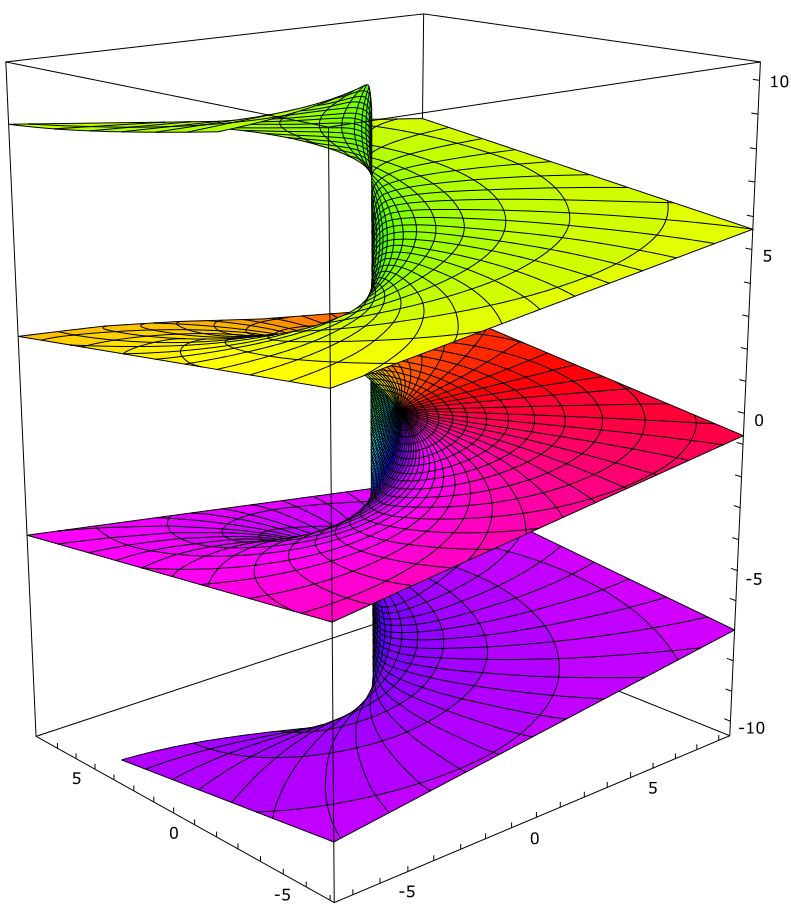
\includegraphics[width=0.45\textwidth]{Riemann.png}
\end{center}
If we set 
\[ \hat f : R \to \C : (z, k) \mapsto \ln|z| + i(\arg_0 z + 2\pi k), \]
we obtain a single-valued function that is analytic with respect to the "natural complex structure" 
on $R$ that is equal to the analytic branch $L_{2\pi k}(z)$ of $\log z$ on the slice 
$\C^* \times \{k\}$. Of course, one would have the clearly describe what is meant by a 
"complex structure" on $R$, but this is beyond the scope of the course. 

Finally, we note that more information on Riemann surfaces can be found in the following books. 
\begin{enumerate}
    \item O. Forster, {\it Lectures on Riemann Surfaces}, Springer-Verlag, 1981. 
    \item S. K. Donaldson, {\it Riemann Surfaces}, Oxford University Press, 2011. 
    \item R. Narasimhan, {\it Compact Riemann Surfaces}, Birh\"auser, 1992. 
\end{enumerate}

\end{document}